\pagebreak
\subsection{Native NetCDF ATM\_SURFACE\_TEMP\_HUM\_WIND\_PRES}
\newp
\begin{longtable}{|p{0.1\textwidth}|p{0.5\textwidth}|}
\caption{Variables in the dataset ATM\_SURFACE\_TEMP\_HUM\_WIND\_PRES}
\label{tab:table-ATM_SURFACE_TEMP_HUM_WIND_PRES-fields} \\ 
\hline \endhead \hline \endfoot
\rowcolor{lightgray} \textbf{Dataset:} & \textbf{ATM\_SURFACE\_TEMP\_HUM\_WIND\_PRES} \\ \hline
Field: &EXFatemp \\ \hline
Field: &EXFaqh \\ \hline
Field: &EXFuwind \\ \hline
Field: &EXFvwind \\ \hline
Field: &EXFwspee \\ \hline
Field: &EXFpress \\ \hline
\end{longtable}

\pagebreak
\subsubsection{Native Variable EXFaqh}
\begin{longtable}{|p{0.06\textwidth}|p{0.41\textwidth}|p{0.39\textwidth}|p{0.06\textwidth}|}
\caption{CDL description of ATM\_SURFACE\_TEMP\_HUM\_WIND\_PRES's EXFaqh variable}
\label{tab:table-ATM_SURFACE_TEMP_HUM_WIND_PRES_EXFaqh} \\ 
\hline \endhead \hline \endfoot
\rowcolor{lightgray} \textbf{Storage Type} & \textbf{Variable Name} & \textbf{Description} & \textbf{Unit} \\ \hline
float32 & EXFaqh & Atmosphere surface (2 m) specific humidity  & kg kg-1 \\ \hline
\rowcolor{lightgray}  \multicolumn{4}{|p{1.00\textwidth}|}{\textbf{CDL Description}} \\ \hline
\multicolumn{4}{|p{1.00\textwidth}|}{\makecell{\parbox{1\textwidth}{float32 EXFaqh(time, tile, j, i)\\
\hspace*{0.5cm}EXFaqh: \_FillValue = 9.96921e+36\\
\hspace*{0.5cm}EXFaqh: long\_name = Atmosphere surface (2 m) specific humidity \\
\hspace*{0.5cm}EXFaqh: units = kg kg: 1\\
\hspace*{0.5cm}EXFaqh: coverage\_content\_type = modelResult\\
\hspace*{0.5cm}EXFaqh: standard\_name = surface\_specific\_humidity\\
\hspace*{0.5cm}EXFaqh: coordinates = time XC YC\\
\hspace*{0.5cm}EXFaqh: valid\_min = : 0.0014020215021446347\\
\hspace*{0.5cm}EXFaqh: valid\_max = 0.03014513850212097}}} \\ \hline
\rowcolor{lightgray} \multicolumn{4}{|p{1.00\textwidth}|}{\textbf{Comments}} \\ \hline
\multicolumn{4}{|p{1\textwidth}|}{Surface (2 m) specific humidity over open water. Note: sum of ERA-Interim surface specific humidity and the control adjustment from ocean state estimation.} \\ \hline
\end{longtable}

\begin{figure}[H]
\centering
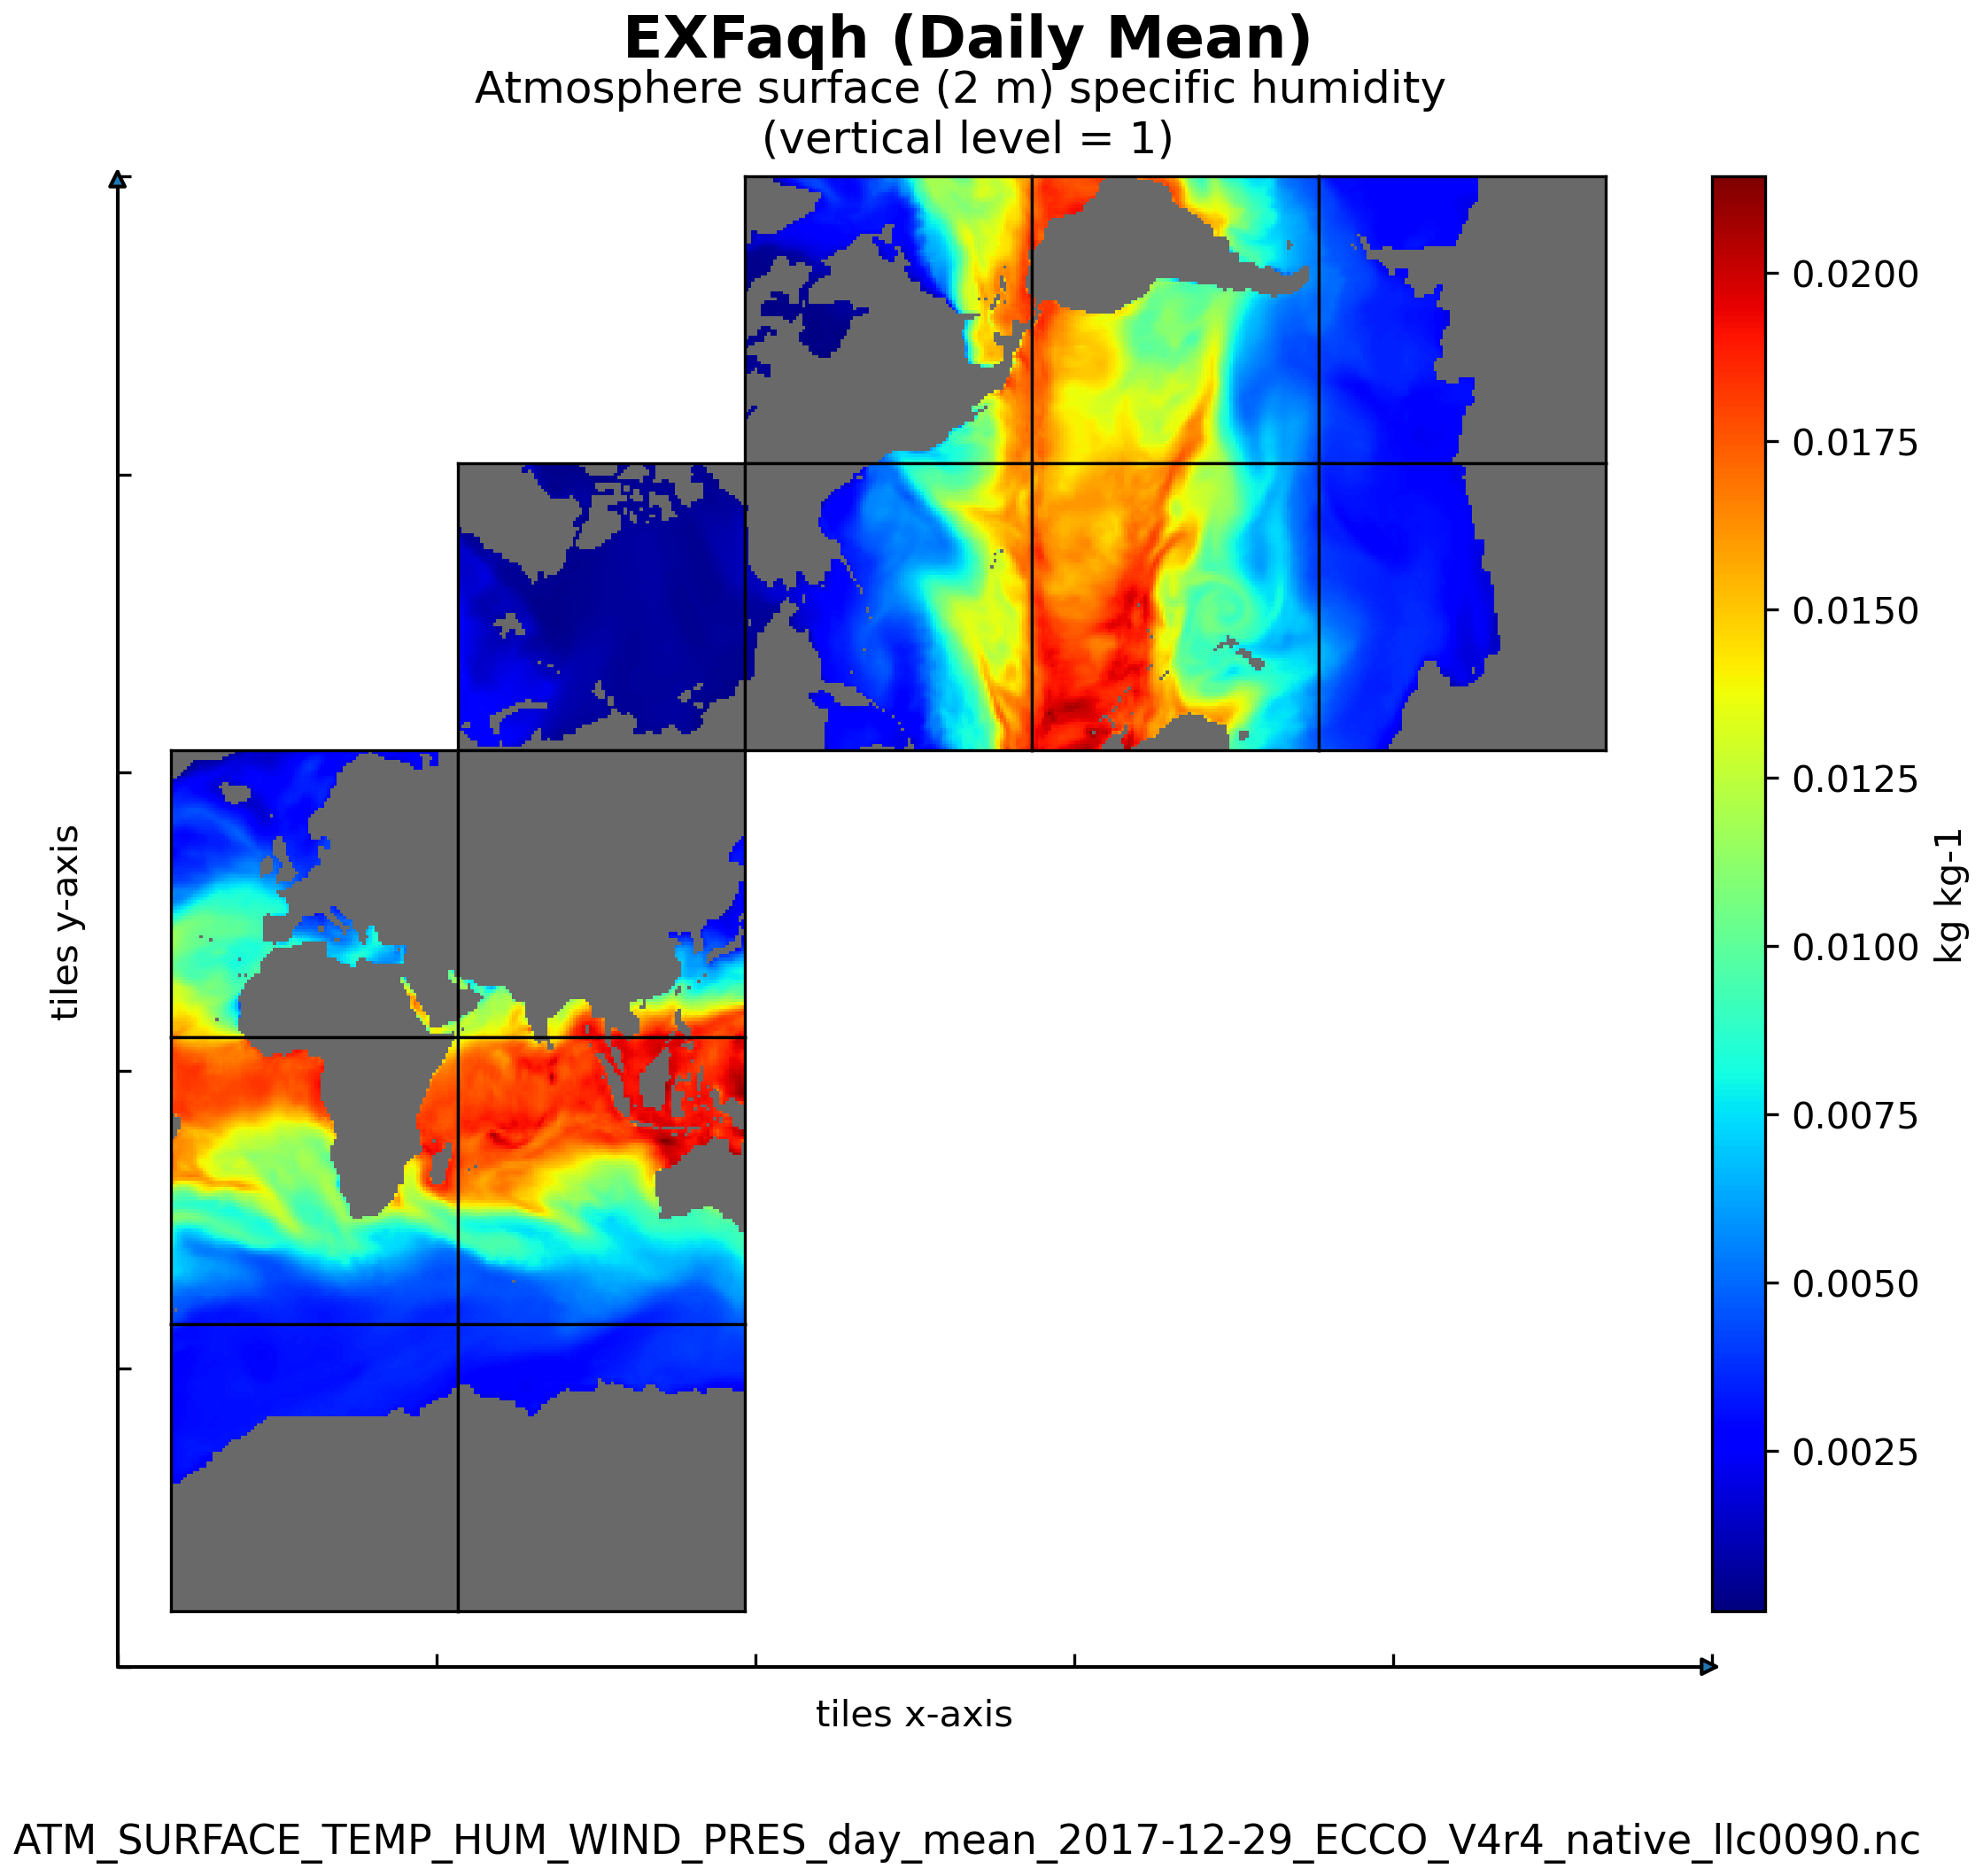
\includegraphics[scale=0.5]{../images/plots/native_plots/Atmosphere_Surface_Temperature_Humidity_Wind_and_Pressure/EXFaqh.png}
\caption{\\Dataset: ATM\_SURFACE\_TEMP\_HUM\_WIND\_PRES\\Variable: EXFaqh}
\label{tab:table-ATM_SURFACE_TEMP_HUM_WIND_PRES_EXFaqh-Plot}
\end{figure}
\pagebreak
\subsubsection{Native Variable EXFatemp}
\begin{longtable}{|p{0.06\textwidth}|p{0.41\textwidth}|p{0.39\textwidth}|p{0.06\textwidth}|}
\caption{CDL description of ATM\_SURFACE\_TEMP\_HUM\_WIND\_PRES's EXFatemp variable}
\label{tab:table-ATM_SURFACE_TEMP_HUM_WIND_PRES_EXFatemp} \\ 
\hline \endhead \hline \endfoot
\rowcolor{lightgray} \textbf{Storage Type} & \textbf{Variable Name} & \textbf{Description} & \textbf{Unit} \\ \hline
float32 & EXFatemp & Atmosphere surface (2 m) air temperature  & degree\_K \\ \hline
\rowcolor{lightgray}  \multicolumn{4}{|p{1.00\textwidth}|}{\textbf{CDL Description}} \\ \hline
\multicolumn{4}{|p{1.00\textwidth}|}{\makecell{\parbox{1\textwidth}{float32 EXFatemp(time, tile, j, i)\\
\hspace*{0.5cm}EXFatemp: \_FillValue = 9.96921e+36\\
\hspace*{0.5cm}EXFatemp: long\_name = Atmosphere surface (2 m) air temperature \\
\hspace*{0.5cm}EXFatemp: units = degree\_K\\
\hspace*{0.5cm}EXFatemp: coverage\_content\_type = modelResult\\
\hspace*{0.5cm}EXFatemp: standard\_name = air\_temperature\\
\hspace*{0.5cm}EXFatemp: coordinates = time XC YC\\
\hspace*{0.5cm}EXFatemp: valid\_min = 195.37054443359375\\
\hspace*{0.5cm}EXFatemp: valid\_max = 312.8451232910156}}} \\ \hline
\rowcolor{lightgray} \multicolumn{4}{|p{1.00\textwidth}|}{\textbf{Comments}} \\ \hline
\multicolumn{4}{|p{1\textwidth}|}{Surface (2 m) air temperature over open water. Note: sum of ERA-Interim surface air temperature and the control adjustment from ocean state estimation.} \\ \hline
\end{longtable}

\begin{figure}[H]
\centering
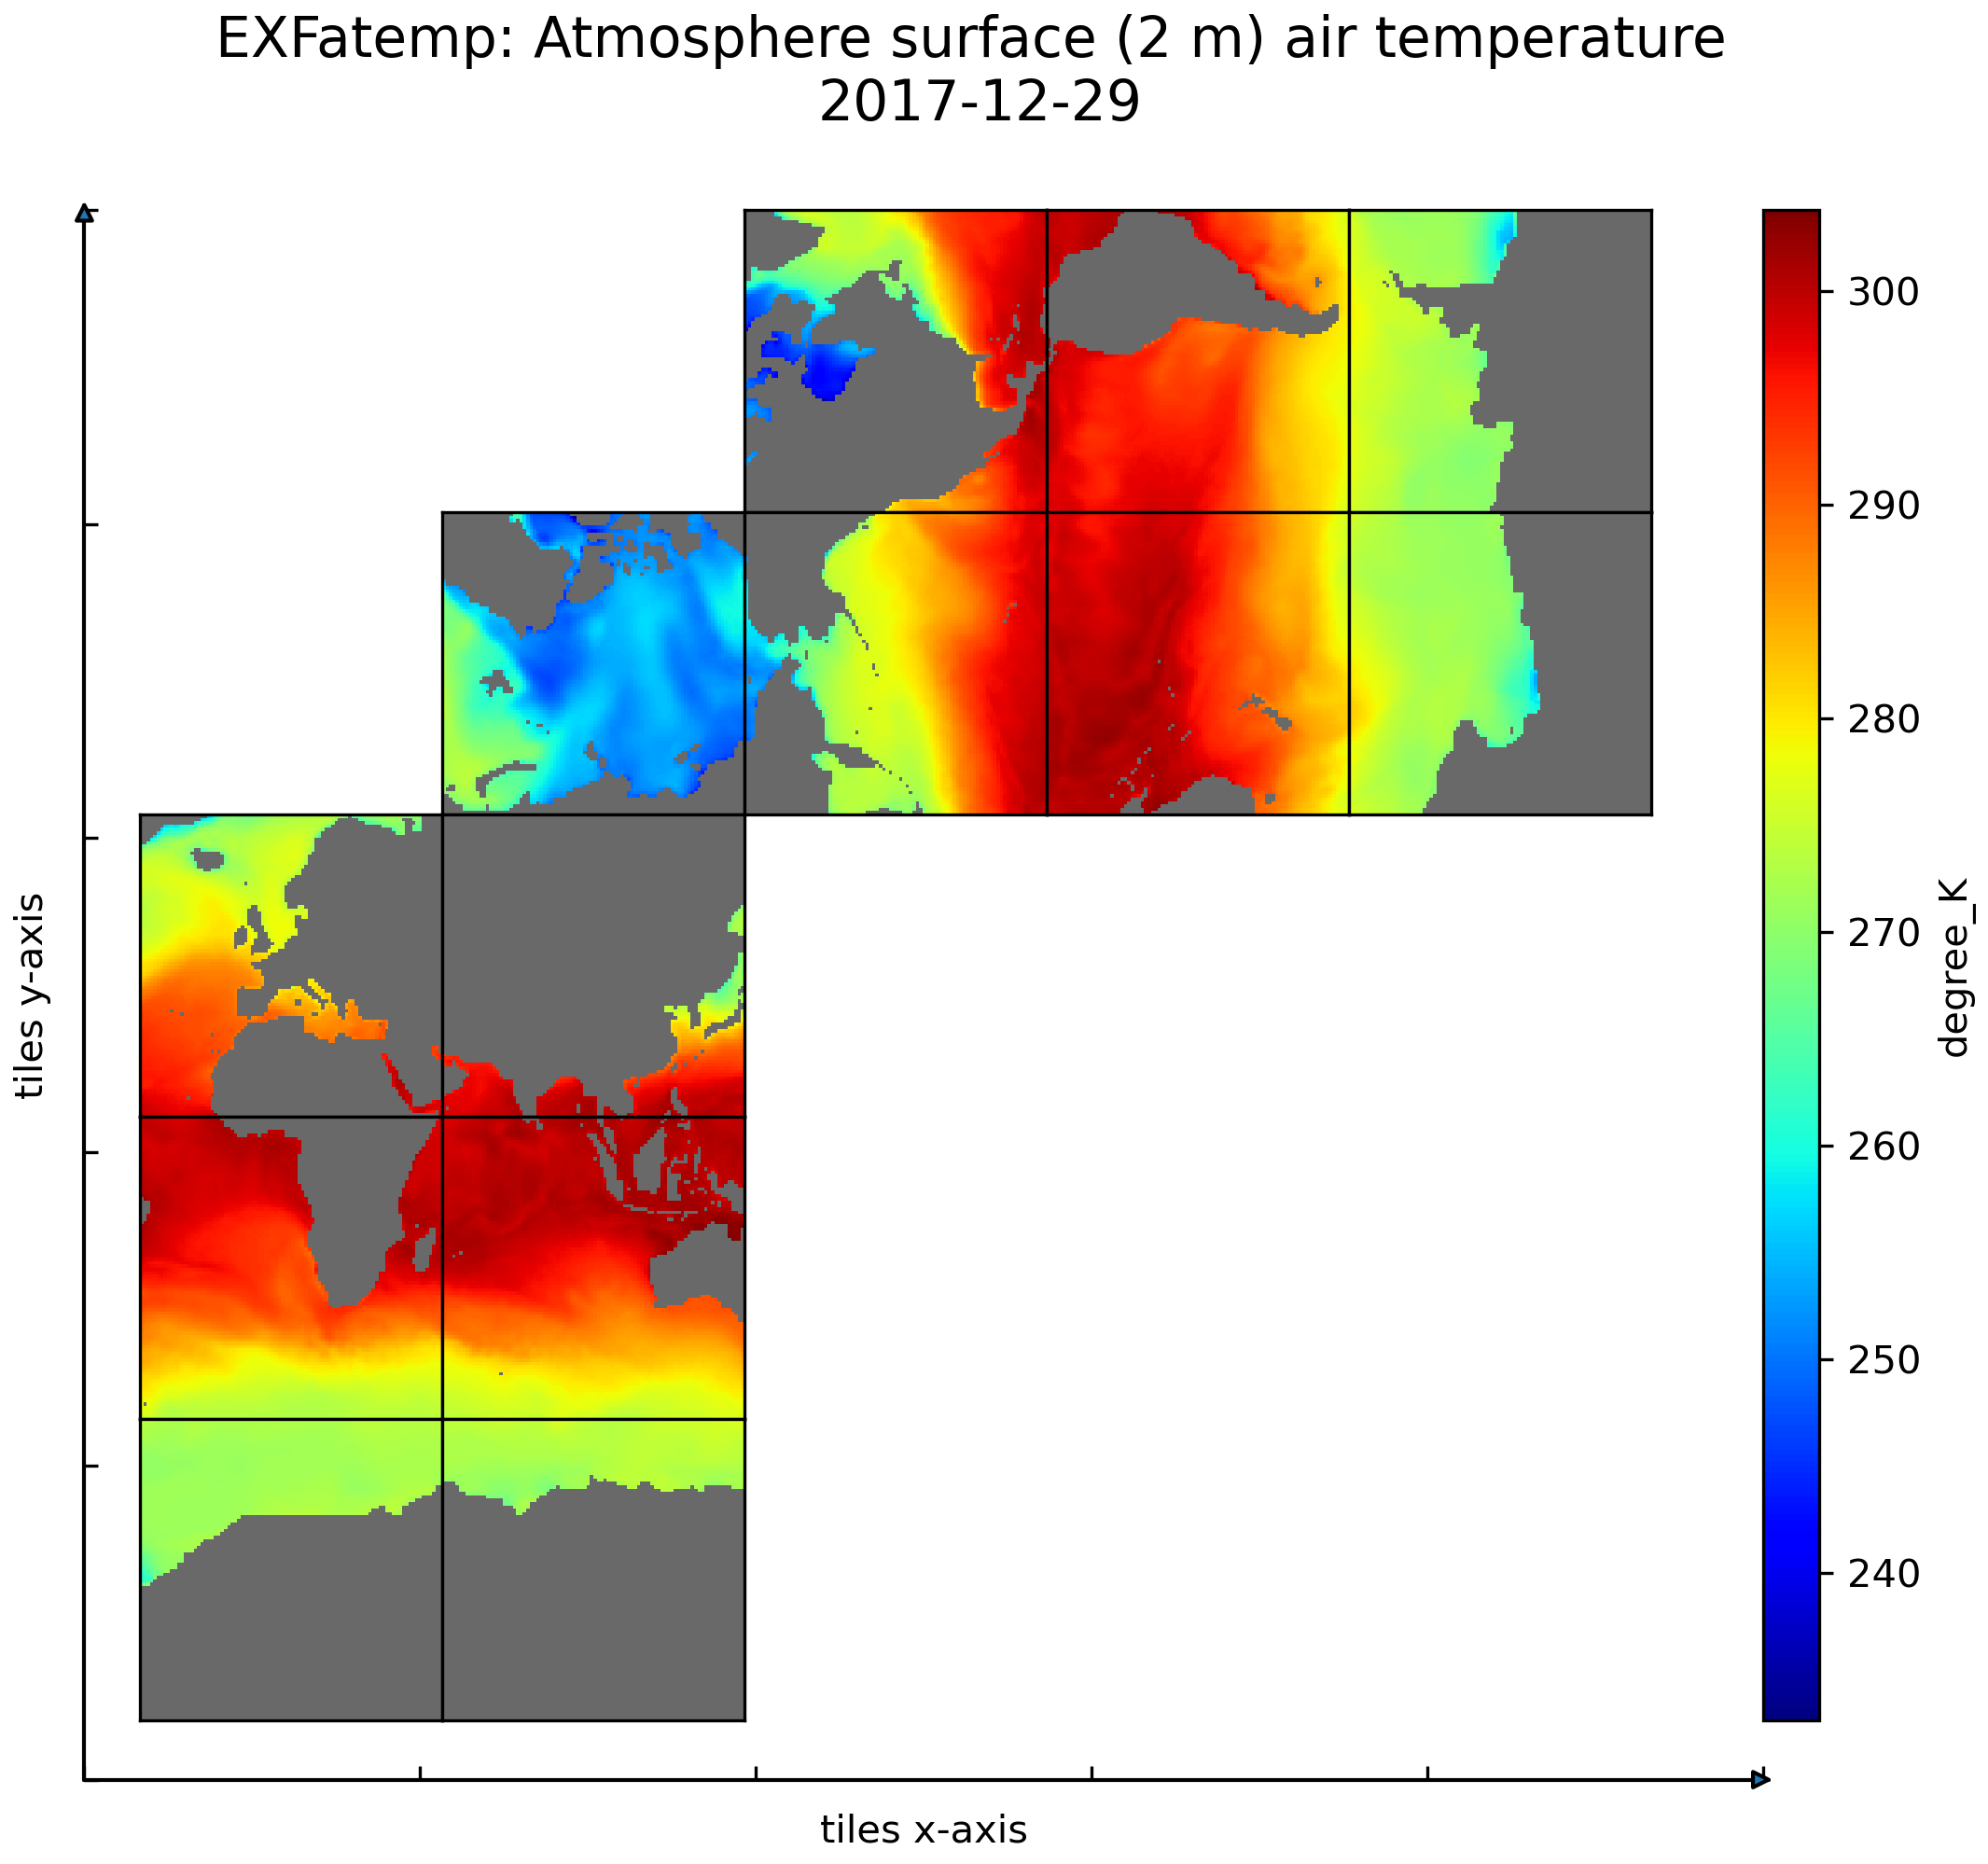
\includegraphics[scale=0.5]{../images/plots/native_plots/Atmosphere_Surface_Temperature_Humidity_Wind_and_Pressure/EXFatemp.png}
\caption{\\Dataset: ATM\_SURFACE\_TEMP\_HUM\_WIND\_PRES\\Variable: EXFatemp}
\label{tab:table-ATM_SURFACE_TEMP_HUM_WIND_PRES_EXFatemp-Plot}
\end{figure}
\pagebreak
\subsubsection{Native Variable EXFpress}
\begin{longtable}{|p{0.06\textwidth}|p{0.41\textwidth}|p{0.39\textwidth}|p{0.06\textwidth}|}
\caption{CDL description of ATM\_SURFACE\_TEMP\_HUM\_WIND\_PRES's EXFpress variable}
\label{tab:table-ATM_SURFACE_TEMP_HUM_WIND_PRES_EXFpress} \\ 
\hline \endhead \hline \endfoot
\rowcolor{lightgray} \textbf{Storage Type} & \textbf{Variable Name} & \textbf{Description} & \textbf{Unit} \\ \hline
float32 & EXFpress & Atmosphere surface pressure & N m-2 \\ \hline
\rowcolor{lightgray}  \multicolumn{4}{|p{1.00\textwidth}|}{\textbf{CDL Description}} \\ \hline
\multicolumn{4}{|p{1.00\textwidth}|}{\makecell{\parbox{1\textwidth}{float32 EXFpress(time, tile, j, i)\\
\hspace*{0.5cm}EXFpress: \_FillValue = 9.96921e+36\\
\hspace*{0.5cm}EXFpress: long\_name = Atmosphere surface pressure\\
\hspace*{0.5cm}EXFpress: units = N m: 2\\
\hspace*{0.5cm}EXFpress: coverage\_content\_type = modelResult\\
\hspace*{0.5cm}EXFpress: standard\_name = surface\_air\_pressure\\
\hspace*{0.5cm}EXFpress: coordinates = time XC YC\\
\hspace*{0.5cm}EXFpress: valid\_min = 92044.171875\\
\hspace*{0.5cm}EXFpress: valid\_max = 106314.7734375}}} \\ \hline
\rowcolor{lightgray} \multicolumn{4}{|p{1.00\textwidth}|}{\textbf{Comments}} \\ \hline
\multicolumn{4}{|p{1\textwidth}|}{Atmospheric pressure field at sea level. Note: ERA-Interim atmospheric pressure, with air tides removed using a variety of methods. Not adjusted by the ocean state estimation.} \\ \hline
\end{longtable}

\begin{figure}[H]
\centering
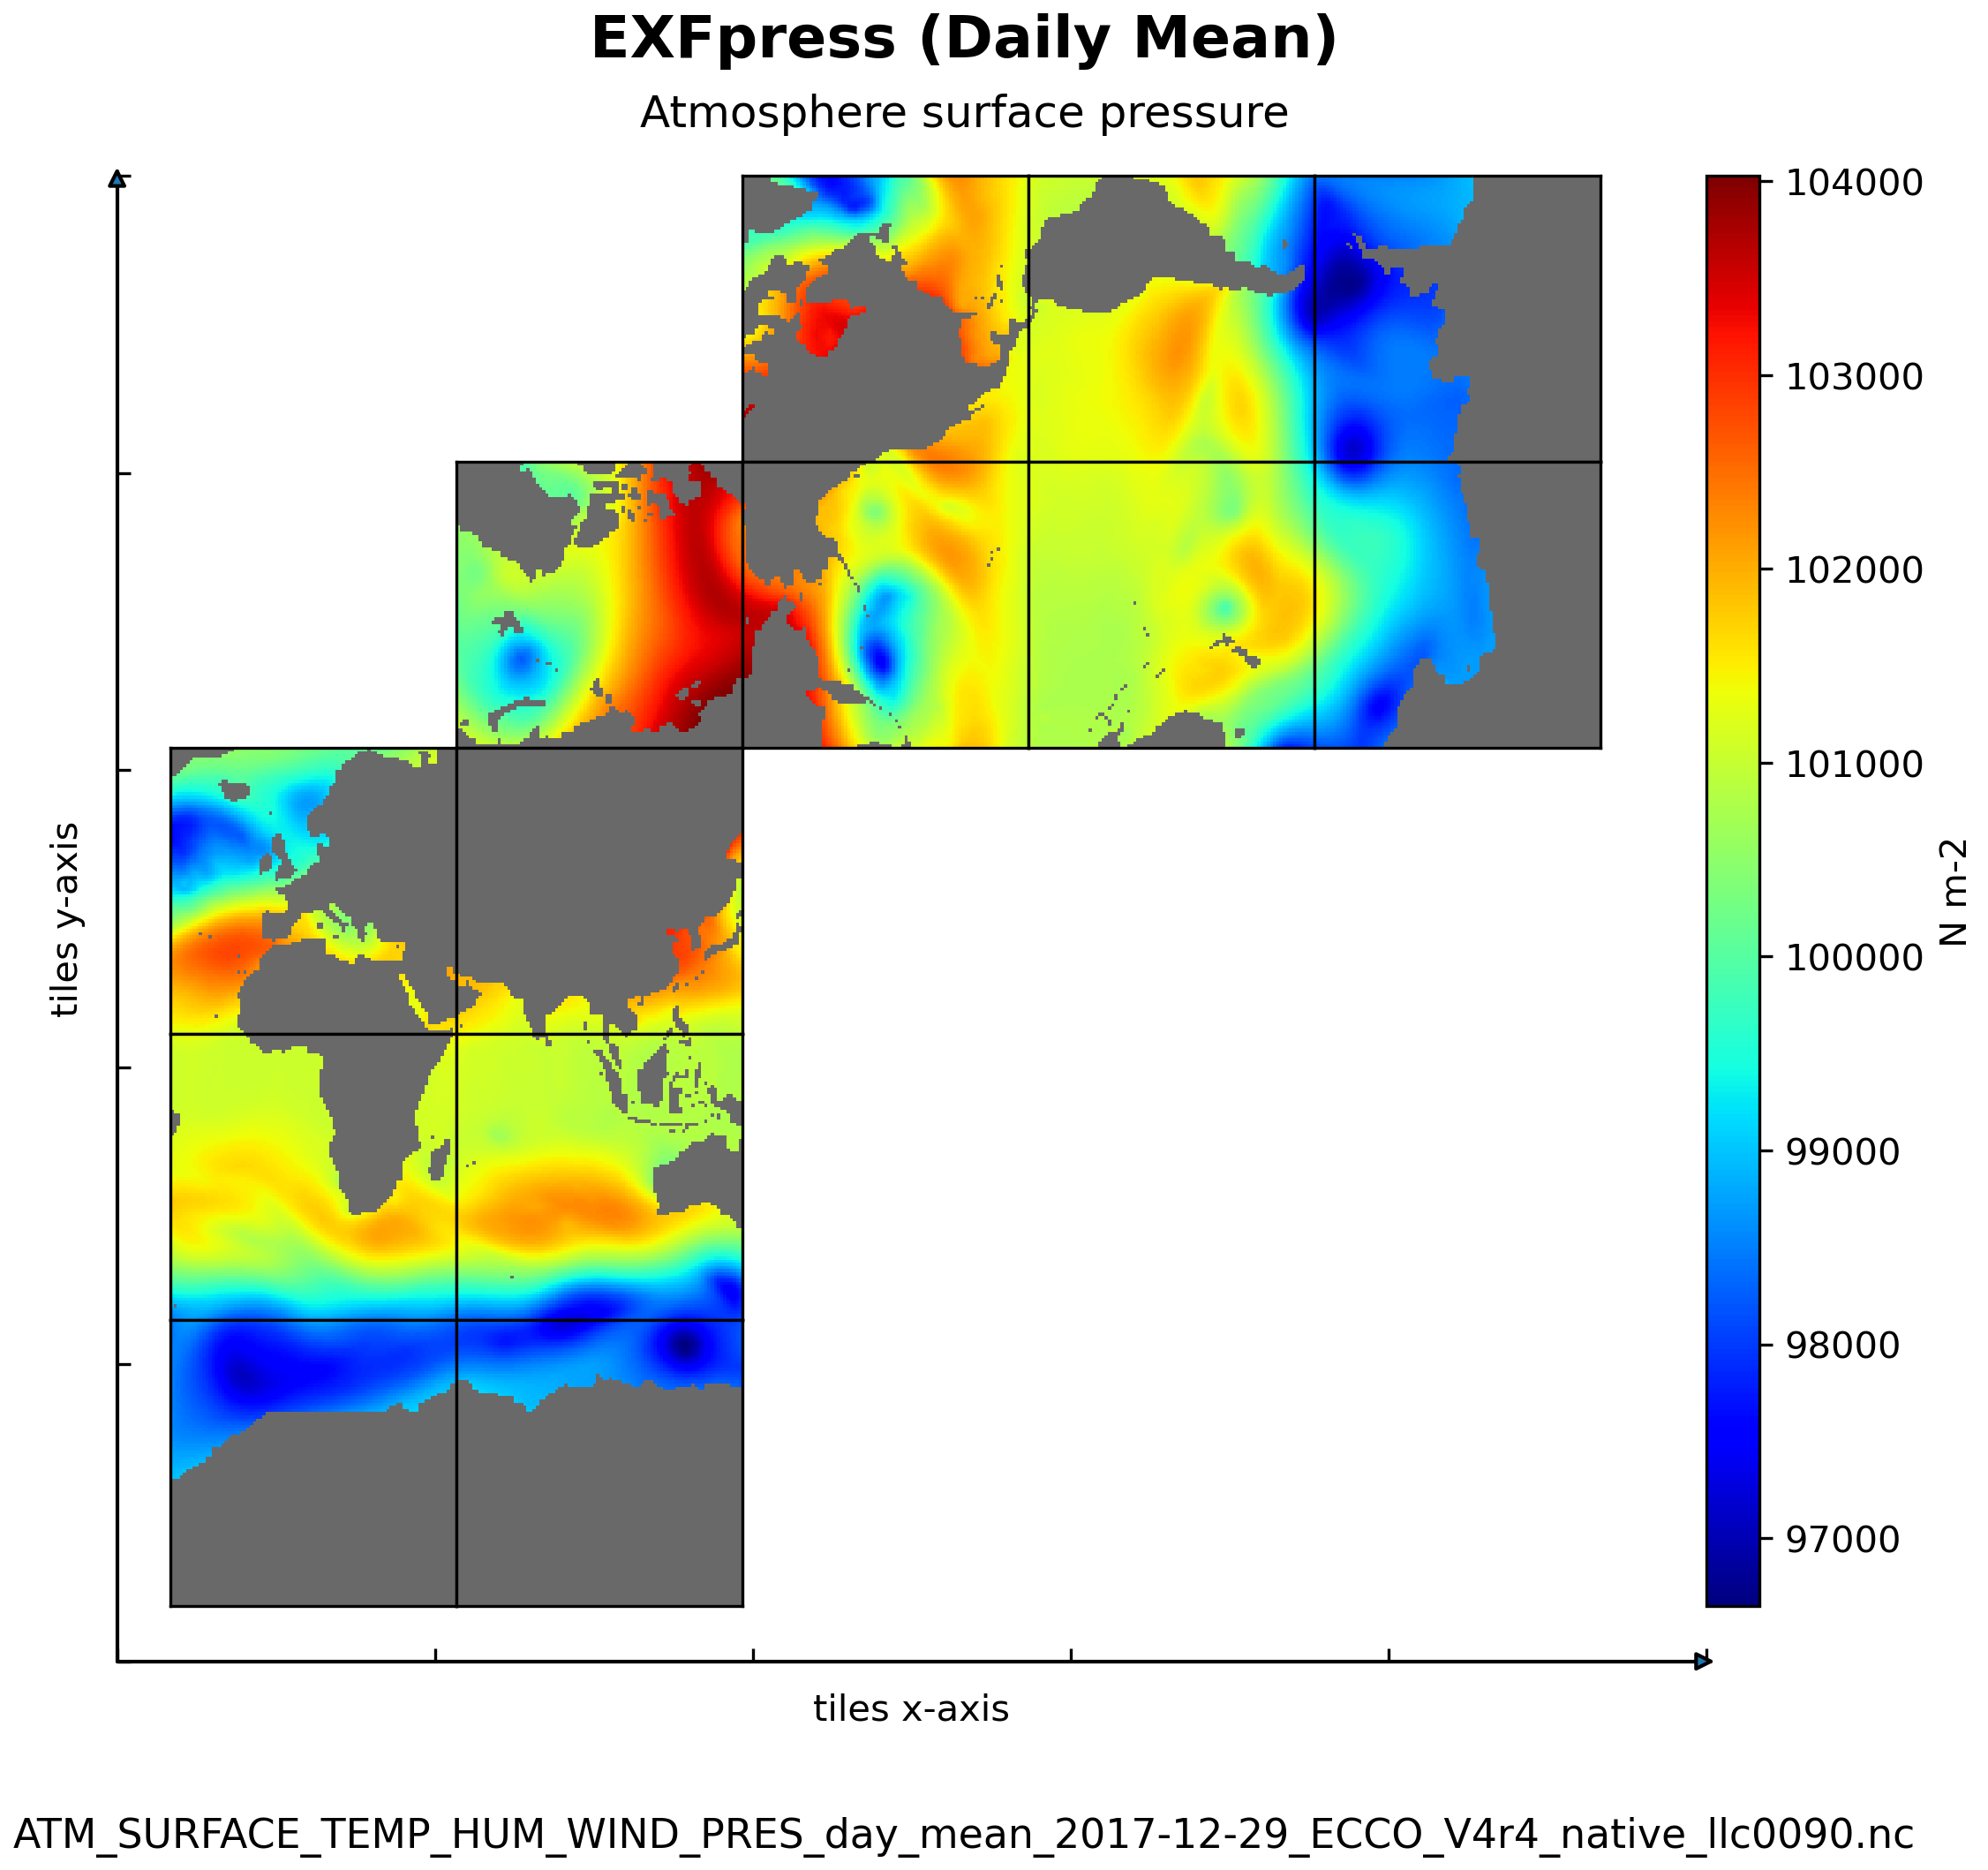
\includegraphics[scale=0.5]{../images/plots/native_plots/Atmosphere_Surface_Temperature_Humidity_Wind_and_Pressure/EXFpress.png}
\caption{\\Dataset: ATM\_SURFACE\_TEMP\_HUM\_WIND\_PRES\\Variable: EXFpress}
\label{tab:table-ATM_SURFACE_TEMP_HUM_WIND_PRES_EXFpress-Plot}
\end{figure}
\pagebreak
\subsubsection{Native Variable EXFuwind}
\begin{longtable}{|p{0.06\textwidth}|p{0.41\textwidth}|p{0.39\textwidth}|p{0.06\textwidth}|}
\caption{CDL description of ATM\_SURFACE\_TEMP\_HUM\_WIND\_PRES's EXFuwind variable}
\label{tab:table-ATM_SURFACE_TEMP_HUM_WIND_PRES_EXFuwind} \\ 
\hline \endhead \hline \endfoot
\rowcolor{lightgray} \textbf{Storage Type} & \textbf{Variable Name} & \textbf{Description} & \textbf{Unit} \\ \hline
float32 & EXFuwind & Wind speed at 10m in the model +x direction & m s-1 \\ \hline
\rowcolor{lightgray}  \multicolumn{4}{|p{1.00\textwidth}|}{\textbf{CDL Description}} \\ \hline
\multicolumn{4}{|p{1.00\textwidth}|}{\makecell{\parbox{1\textwidth}{float32 EXFuwind(time, tile, j, i)\\
\hspace*{0.5cm}EXFuwind: \_FillValue = 9.96921e+36\\
\hspace*{0.5cm}EXFuwind: long\_name = Wind speed at 10m in the model +x direction\\
\hspace*{0.5cm}EXFuwind: units = m s: 1\\
\hspace*{0.5cm}EXFuwind: coverage\_content\_type = modelResult\\
\hspace*{0.5cm}EXFuwind: standard\_name = x\_wind\\
\hspace*{0.5cm}EXFuwind: coordinates = time XC YC\\
\hspace*{0.5cm}EXFuwind: valid\_min = : 34.528900146484375\\
\hspace*{0.5cm}EXFuwind: valid\_max = 29.92486572265625}}} \\ \hline
\rowcolor{lightgray} \multicolumn{4}{|p{1.00\textwidth}|}{\textbf{Comments}} \\ \hline
\multicolumn{4}{|p{1\textwidth}|}{Wind speed at 10m in the +x direction at the tracer cell on the native model grid. Note: ECCO v4r4 is forced with wind stress (see EXFtaux) not vector winds converted to wind stress using bulk formulae. EXFuwind is calculated by converting wind stress to vector wind using bulk formulae.} \\ \hline
\end{longtable}

\begin{figure}[H]
\centering
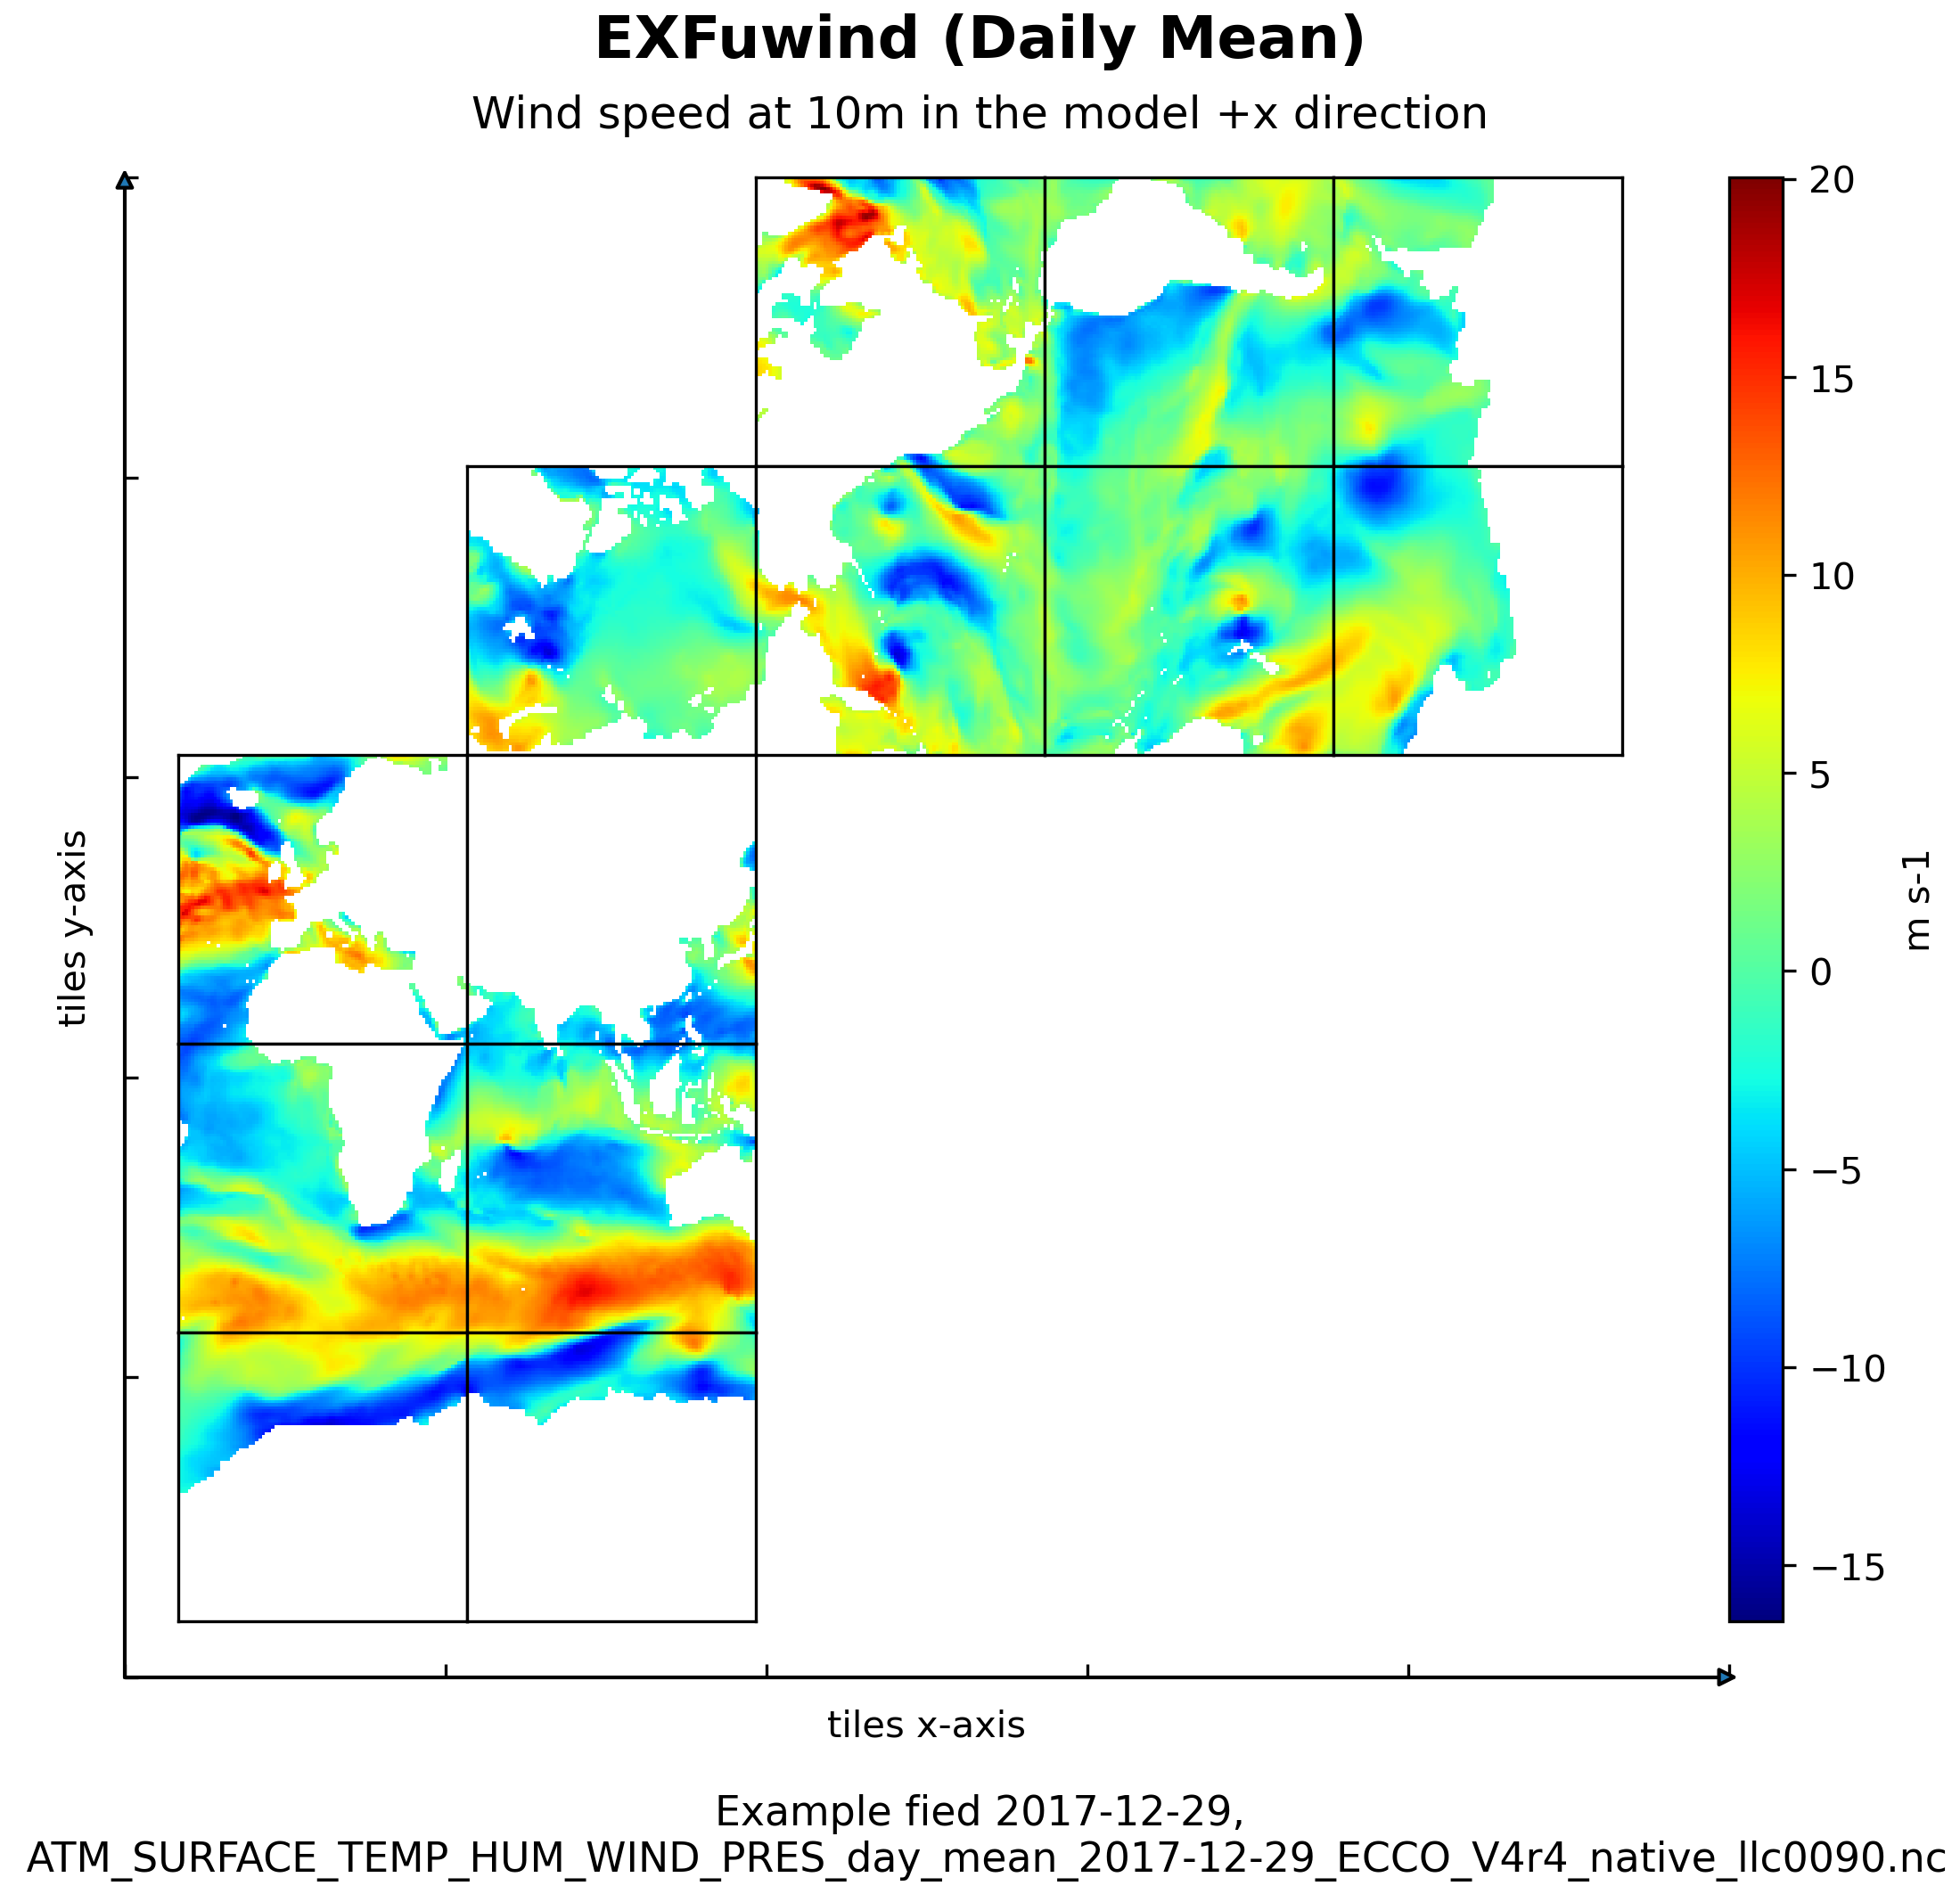
\includegraphics[scale=0.5]{../images/plots/native_plots/Atmosphere_Surface_Temperature_Humidity_Wind_and_Pressure/EXFuwind.png}
\caption{\\Dataset: ATM\_SURFACE\_TEMP\_HUM\_WIND\_PRES\\Variable: EXFuwind}
\label{tab:table-ATM_SURFACE_TEMP_HUM_WIND_PRES_EXFuwind-Plot}
\end{figure}
\pagebreak
\subsubsection{Native Variable EXFvwind}
\begin{longtable}{|p{0.06\textwidth}|p{0.41\textwidth}|p{0.39\textwidth}|p{0.06\textwidth}|}
\caption{CDL description of ATM\_SURFACE\_TEMP\_HUM\_WIND\_PRES's EXFvwind variable}
\label{tab:table-ATM_SURFACE_TEMP_HUM_WIND_PRES_EXFvwind} \\ 
\hline \endhead \hline \endfoot
\rowcolor{lightgray} \textbf{Storage Type} & \textbf{Variable Name} & \textbf{Description} & \textbf{Unit} \\ \hline
float32 & EXFvwind & Wind speed at 10m in the model +y direction & m s-1 \\ \hline
\rowcolor{lightgray}  \multicolumn{4}{|p{1.00\textwidth}|}{\textbf{CDL Description}} \\ \hline
\multicolumn{4}{|p{1.00\textwidth}|}{\makecell{\parbox{1\textwidth}{float32 EXFvwind(time, tile, j, i)\\
\hspace*{0.5cm}EXFvwind: \_FillValue = 9.96921e+36\\
\hspace*{0.5cm}EXFvwind: long\_name = Wind speed at 10m in the model +y direction\\
\hspace*{0.5cm}EXFvwind: units = m s: 1\\
\hspace*{0.5cm}EXFvwind: coverage\_content\_type = modelResult\\
\hspace*{0.5cm}EXFvwind: standard\_name = y\_wind\\
\hspace*{0.5cm}EXFvwind: coordinates = time XC YC\\
\hspace*{0.5cm}EXFvwind: valid\_min = : 27.9254093170166\\
\hspace*{0.5cm}EXFvwind: valid\_max = 45.065101623535156}}} \\ \hline
\rowcolor{lightgray} \multicolumn{4}{|p{1.00\textwidth}|}{\textbf{Comments}} \\ \hline
\multicolumn{4}{|p{1\textwidth}|}{Wind speed at 10m in the +y direction at the tracer cell on the native model grid. Note: ECCO v4r4 is forced with wind stress (see EXFtauy) not vector winds converted to wind stress using bulk formulae. EXFvwind is calculated by converting wind stress to vector wind using bulk formulae.} \\ \hline
\end{longtable}

\begin{figure}[H]
\centering
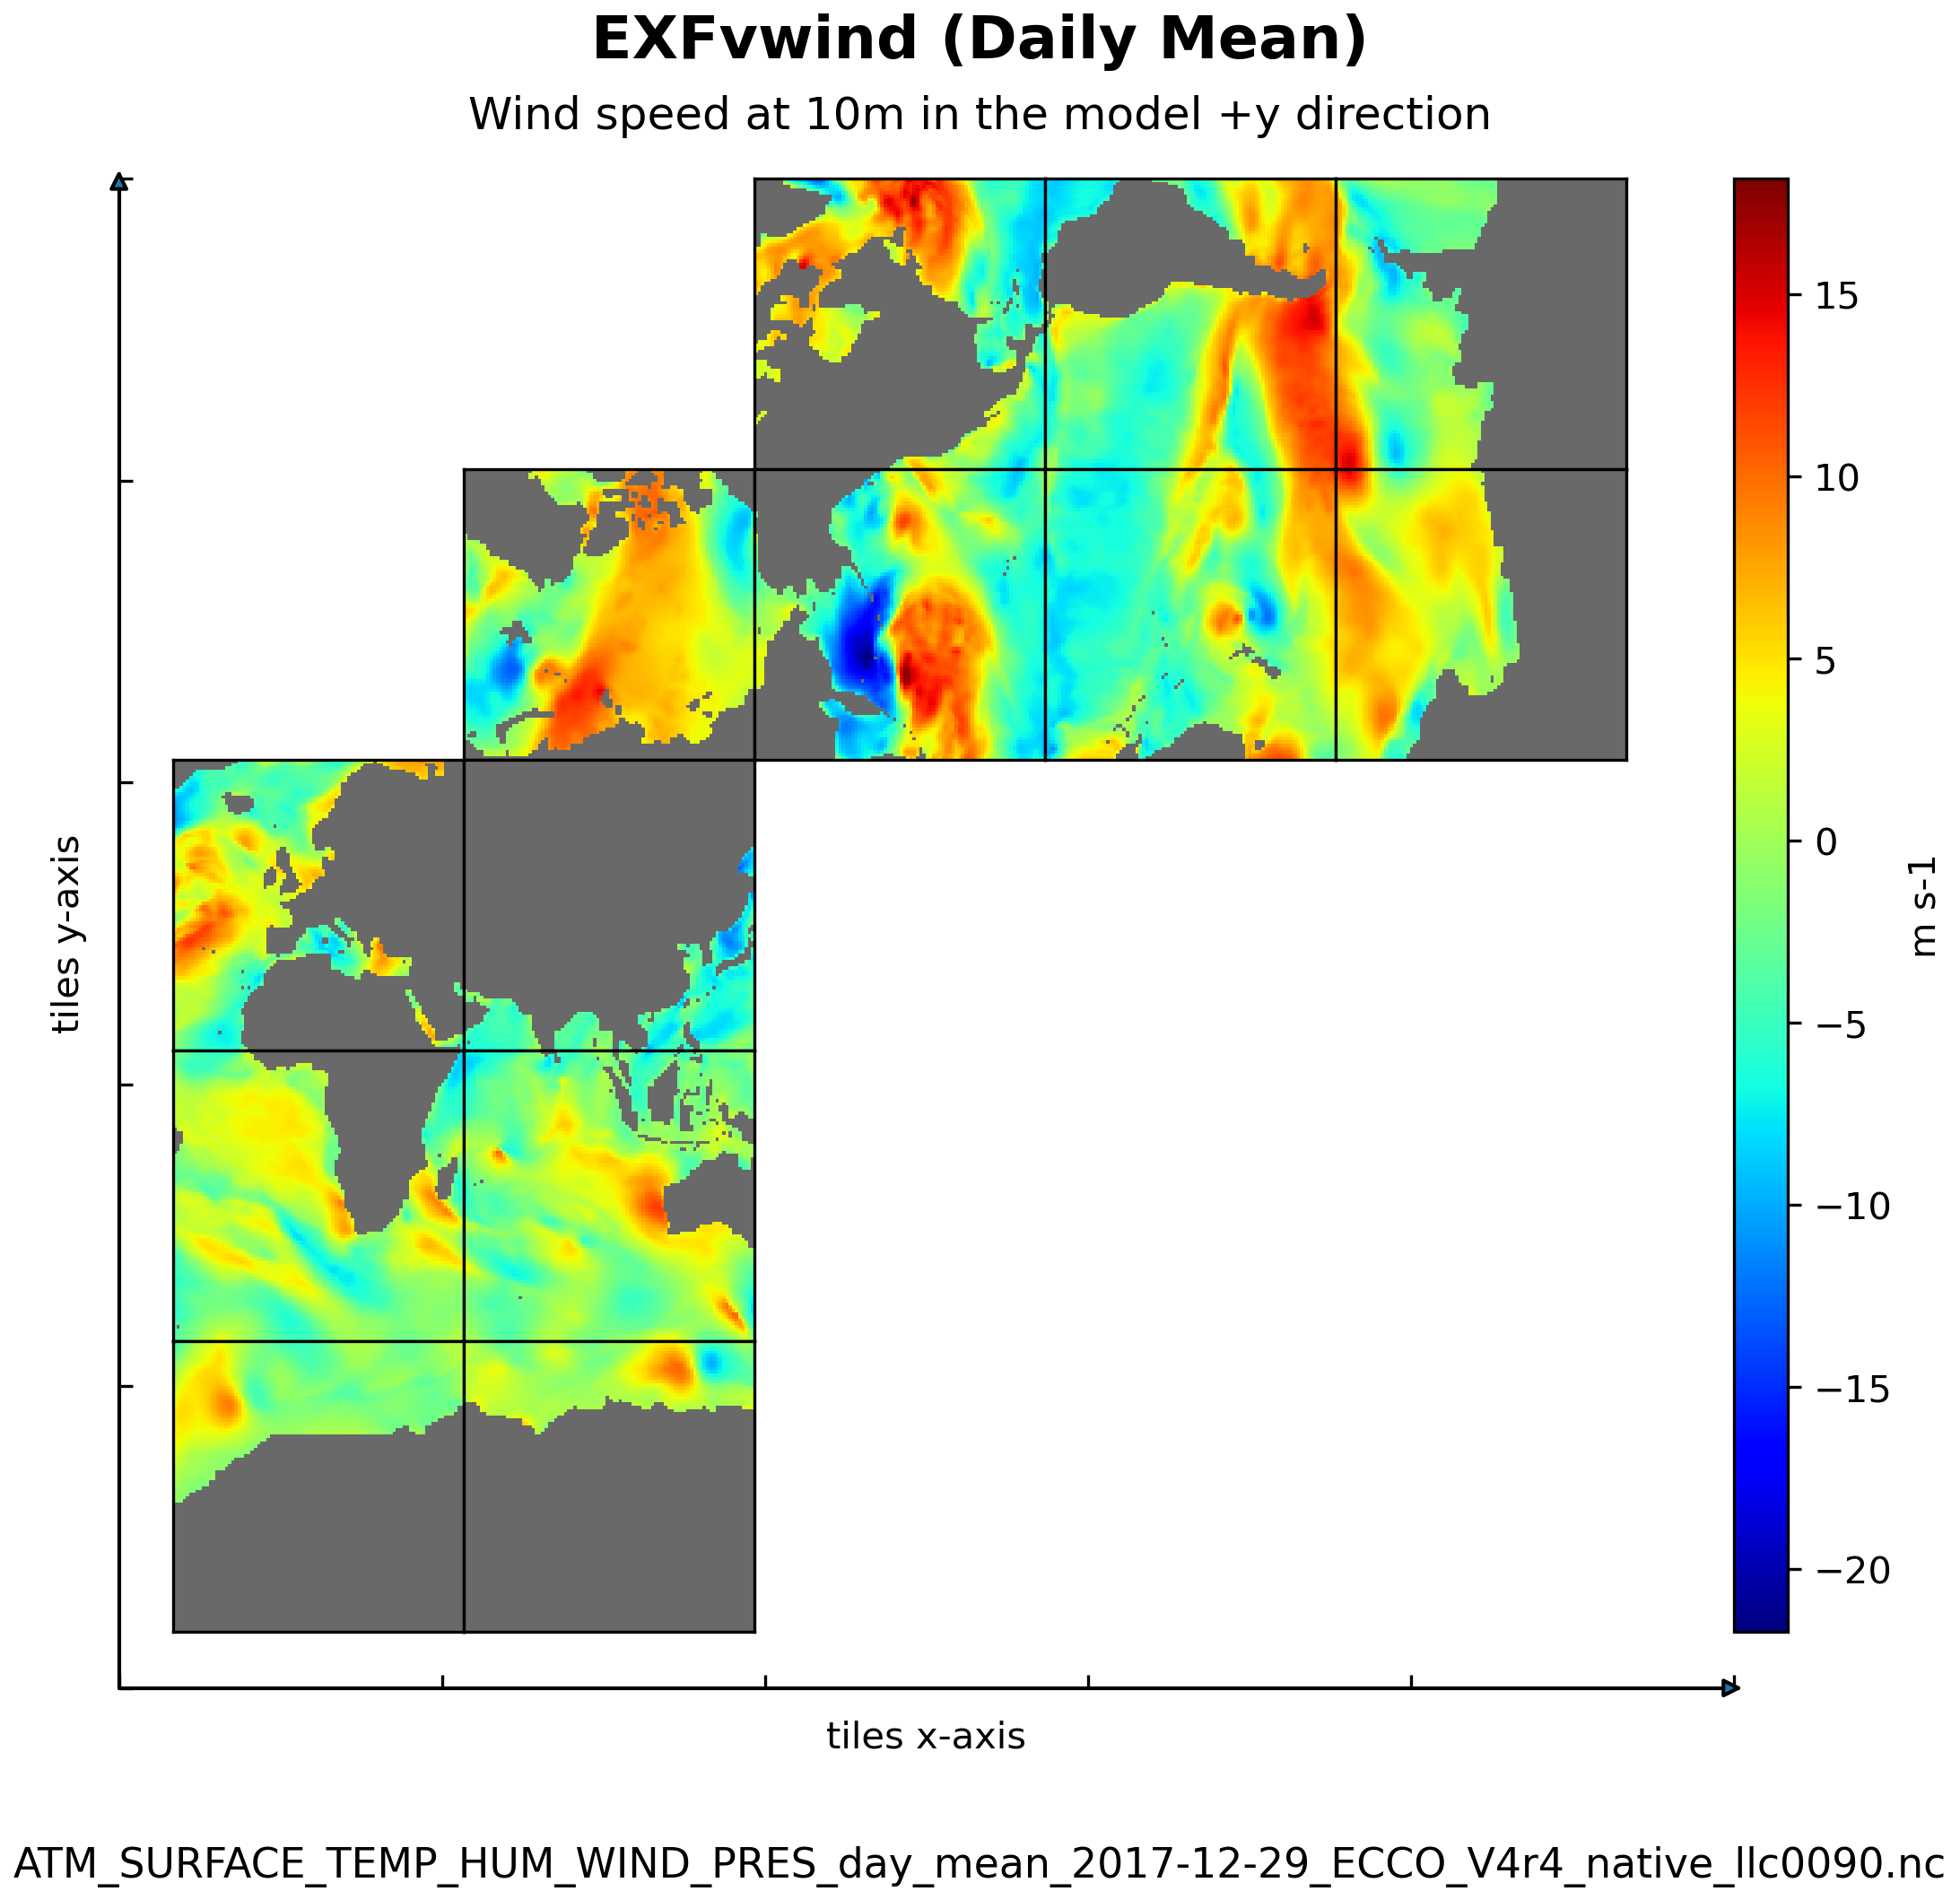
\includegraphics[scale=0.5]{../images/plots/native_plots/Atmosphere_Surface_Temperature_Humidity_Wind_and_Pressure/EXFvwind.png}
\caption{\\Dataset: ATM\_SURFACE\_TEMP\_HUM\_WIND\_PRES\\Variable: EXFvwind}
\label{tab:table-ATM_SURFACE_TEMP_HUM_WIND_PRES_EXFvwind-Plot}
\end{figure}
\pagebreak
\subsubsection{Native Variable EXFwspee}
\begin{longtable}{|p{0.06\textwidth}|p{0.41\textwidth}|p{0.39\textwidth}|p{0.06\textwidth}|}
\caption{CDL description of ATM\_SURFACE\_TEMP\_HUM\_WIND\_PRES's EXFwspee variable}
\label{tab:table-ATM_SURFACE_TEMP_HUM_WIND_PRES_EXFwspee} \\ 
\hline \endhead \hline \endfoot
\rowcolor{lightgray} \textbf{Storage Type} & \textbf{Variable Name} & \textbf{Description} & \textbf{Unit} \\ \hline
float32 & EXFwspee & Wind speed & m s-1 \\ \hline
\rowcolor{lightgray}  \multicolumn{4}{|p{1.00\textwidth}|}{\textbf{CDL Description}} \\ \hline
\multicolumn{4}{|p{1.00\textwidth}|}{\makecell{\parbox{1\textwidth}{float32 EXFwspee(time, tile, j, i)\\
\hspace*{0.5cm}EXFwspee: \_FillValue = 9.96921e+36\\
\hspace*{0.5cm}EXFwspee: long\_name = Wind speed\\
\hspace*{0.5cm}EXFwspee: units = m s: 1\\
\hspace*{0.5cm}EXFwspee: coverage\_content\_type = modelResult\\
\hspace*{0.5cm}EXFwspee: standard\_name = wind\_speed\\
\hspace*{0.5cm}EXFwspee: coordinates = time XC YC\\
\hspace*{0.5cm}EXFwspee: valid\_min = 0.27271032333374023\\
\hspace*{0.5cm}EXFwspee: valid\_max = 45.87086486816406}}} \\ \hline
\rowcolor{lightgray} \multicolumn{4}{|p{1.00\textwidth}|}{\textbf{Comments}} \\ \hline
\multicolumn{4}{|p{1\textwidth}|}{10-m wind speed magnitude (>= 0 ) over open water. Only used for the calculation of air-sea fluxes using bulk formulae. Note: not adjusted by the ocean state estimation and not necesarily consistent with EXFuwind and EXFvwind because EXFuwind and EXFvwind are calculated from EXFtaux and EXFtauy using bulk formulae. EXFwspee != sqrt(EXFuwind**2 + EXFvwind**2.} \\ \hline
\end{longtable}

\begin{figure}[H]
\centering
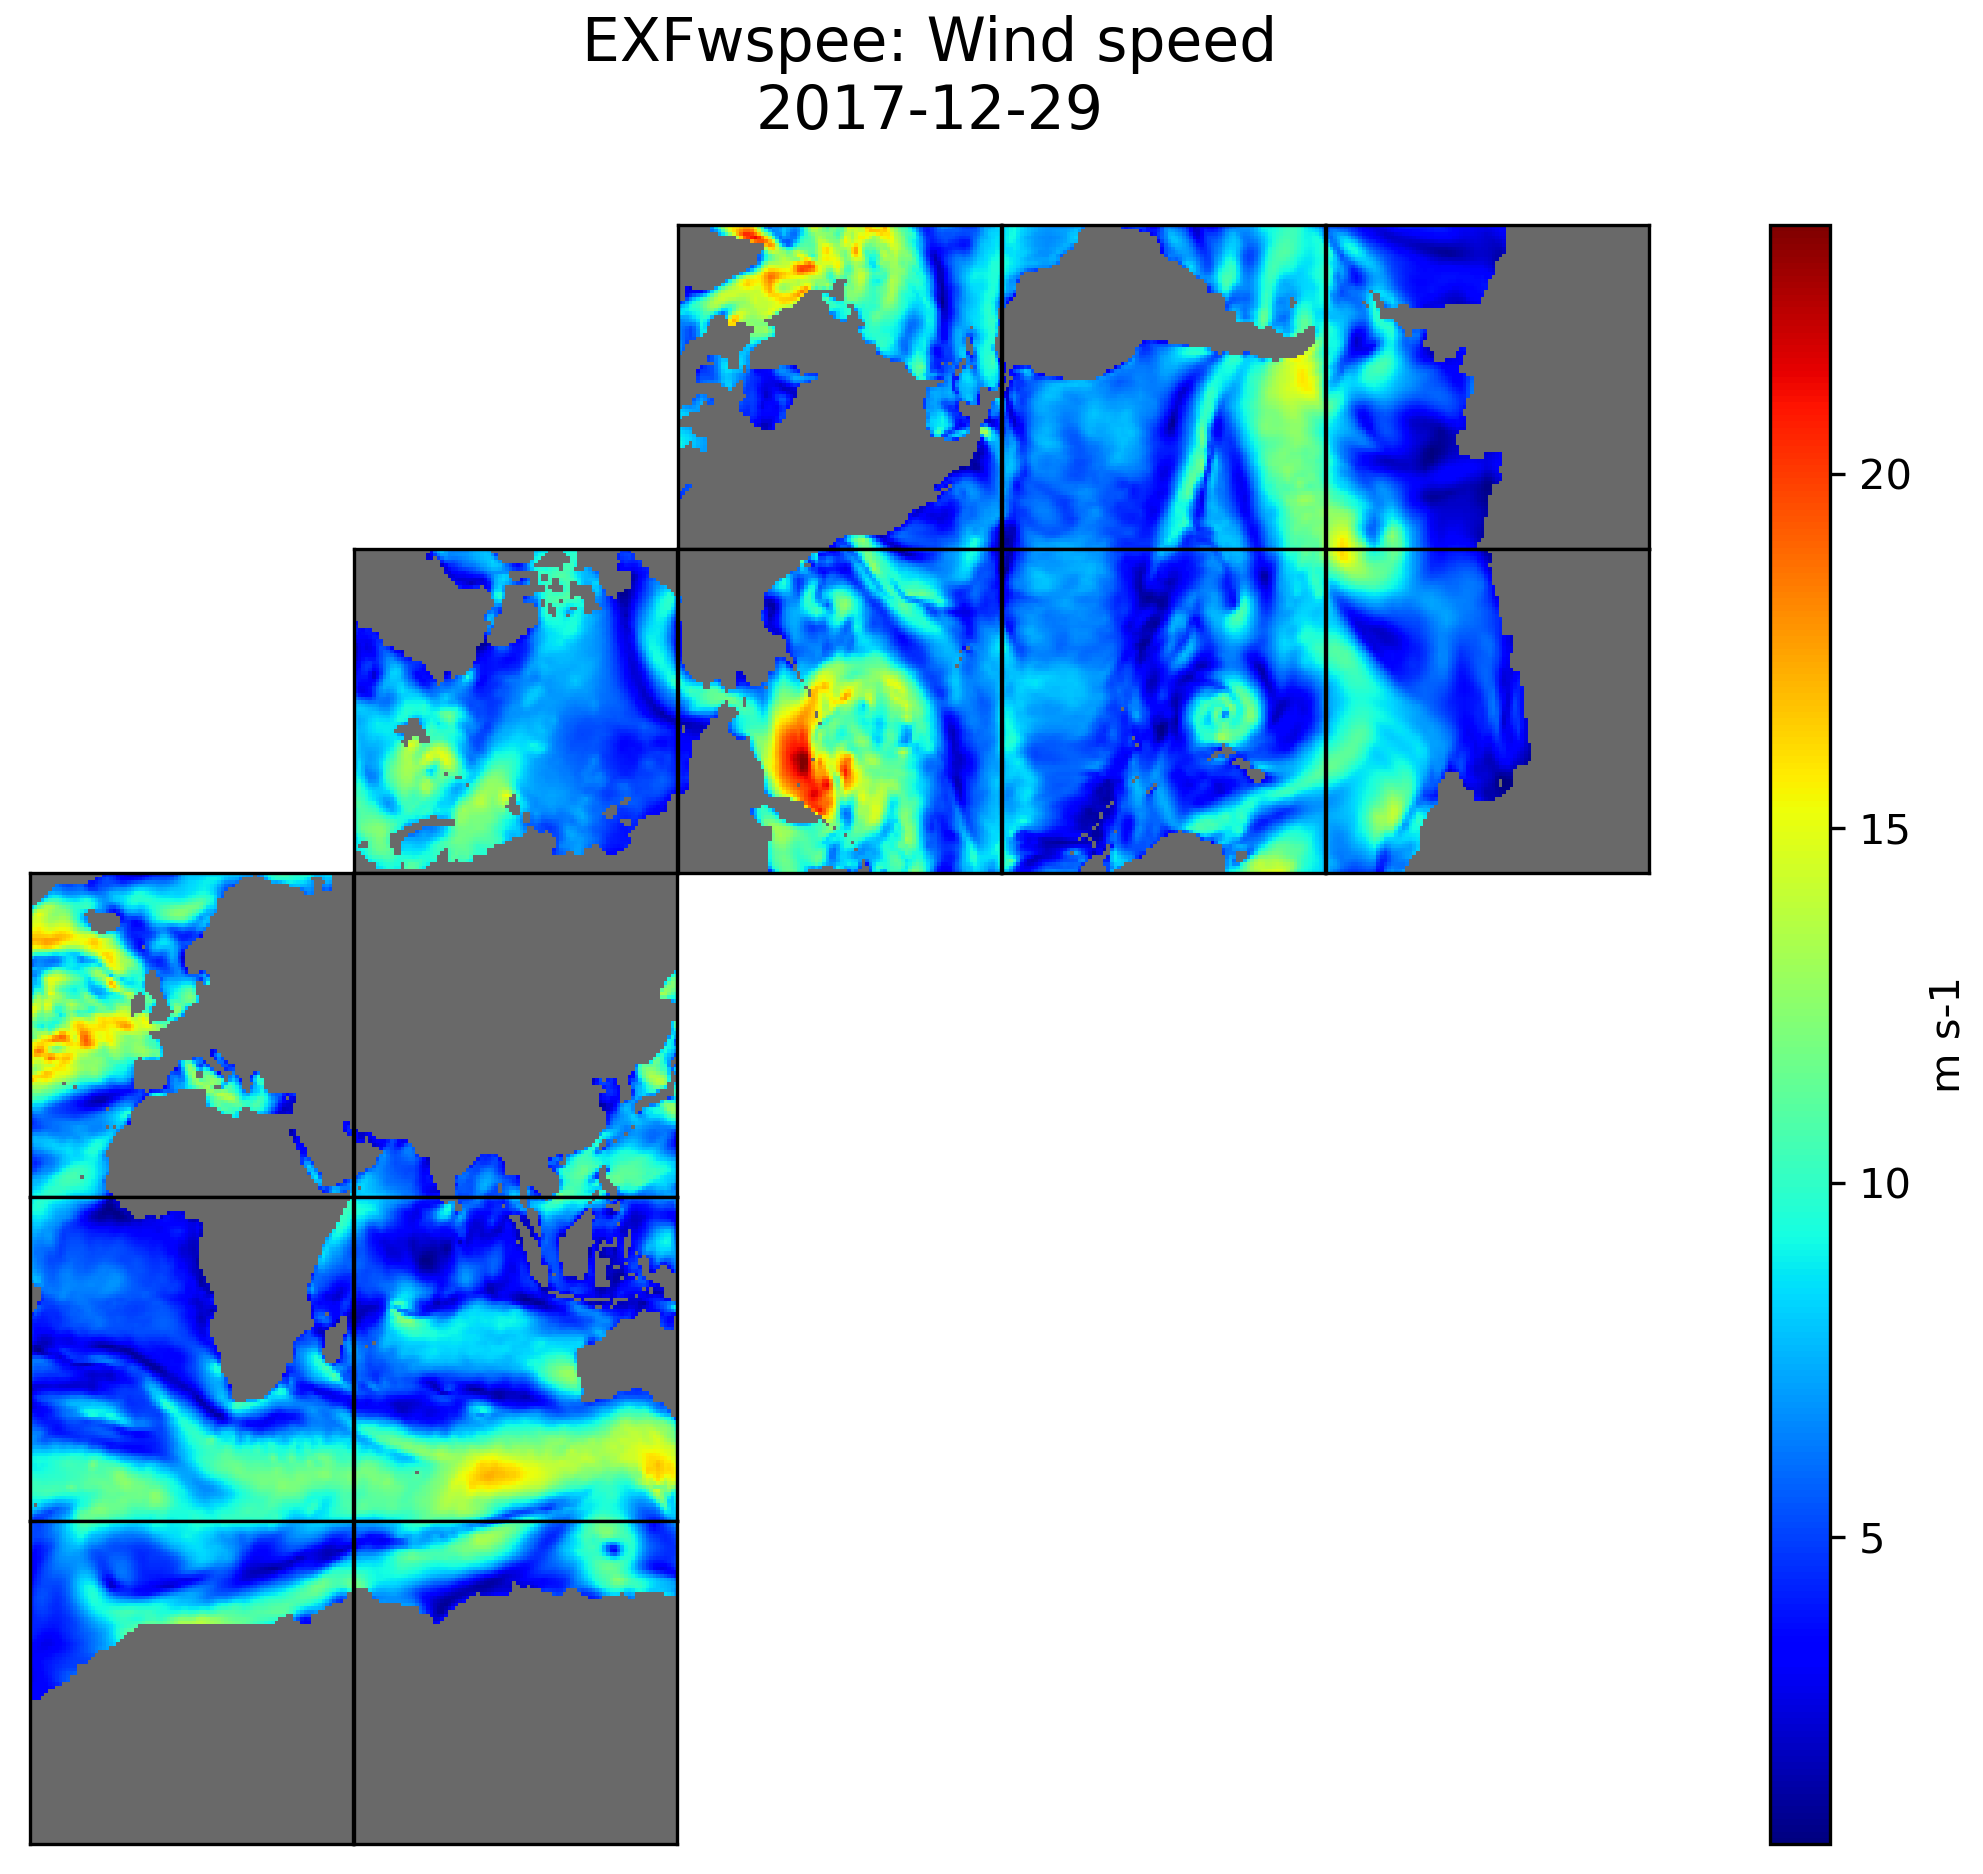
\includegraphics[scale=0.5]{../images/plots/native_plots/Atmosphere_Surface_Temperature_Humidity_Wind_and_Pressure/EXFwspee.png}
\caption{\\Dataset: ATM\_SURFACE\_TEMP\_HUM\_WIND\_PRES\\Variable: EXFwspee}
\label{tab:table-ATM_SURFACE_TEMP_HUM_WIND_PRES_EXFwspee-Plot}
\end{figure}
\pagebreak
\subsection{Native NetCDF OCEAN\_3D\_MIXING\_COEFFS}
\newp
\begin{longtable}{|p{0.1\textwidth}|p{0.5\textwidth}|}
\caption{Variables in the dataset OCEAN\_3D\_MIXING\_COEFFS\_ECCO}
\label{tab:table-OCEAN_3D_MIXING_COEFFS_ECCO-fields} \\ 
\hline \endhead \hline \endfoot
\rowcolor{lightgray} \textbf{Dataset:} & \textbf{OCEAN\_3D\_MIXING\_COEFFS\_ECCO} \\ \hline
Field: &DIFFKR \\ \hline
Field: &KAPGM \\ \hline
Field: &KAPREDI \\ \hline
\end{longtable}

\pagebreak
\subsubsection{Native Variable DIFFKR}
\begin{longtable}{|p{0.06\textwidth}|p{0.41\textwidth}|p{0.39\textwidth}|p{0.06\textwidth}|}
\caption{CDL description of OCEAN\_3D\_MIXING\_COEFFS's DIFFKR variable}
\label{tab:table-OCEAN_3D_MIXING_COEFFS_DIFFKR} \\ 
\hline \endhead \hline \endfoot
\rowcolor{lightgray} \textbf{Storage Type} & \textbf{Variable Name} & \textbf{Description} & \textbf{Unit} \\ \hline
float32 & DIFFKR & Vertical diffusivity & m2 s-1 \\ \hline
\rowcolor{lightgray}  \multicolumn{4}{|p{1.00\textwidth}|}{\textbf{CDL Description}} \\ \hline
\multicolumn{4}{|p{1.00\textwidth}|}{\makecell{\parbox{1\textwidth}{float32 DIFFKR(k, tile, j, i)\\
\hspace*{0.5cm}DIFFKR: \_FillValue = 9.96921e+36\\
\hspace*{0.5cm}DIFFKR: coverage\_content\_type = modelResult\\
\hspace*{0.5cm}DIFFKR: long\_name = Vertical diffusivity\\
\hspace*{0.5cm}DIFFKR: units = m2 s: 1\\
\hspace*{0.5cm}DIFFKR: valid\_min = 1e: 06\\
\hspace*{0.5cm}DIFFKR: valid\_max = 0.0001854995\\
\hspace*{0.5cm}DIFFKR: coordinates = Z XC YC}}} \\ \hline
\rowcolor{lightgray} \multicolumn{4}{|p{1.00\textwidth}|}{\textbf{Comments}} \\ \hline
\multicolumn{4}{|p{1\textwidth}|}{Background vertical diffusion coefficient for temperature and salinity. Total vertical diffusivity includes background diffusivity plus contributions from the GGL90 vertical mixing and the Gent-McWilliams/Redi parameterizations. Note: DIFFKR is a model control variable and has been optimized from a spatially-invariant first-guess value of 1e-5 m2 s-1.} \\ \hline
\end{longtable}

\begin{figure}[H]
\centering
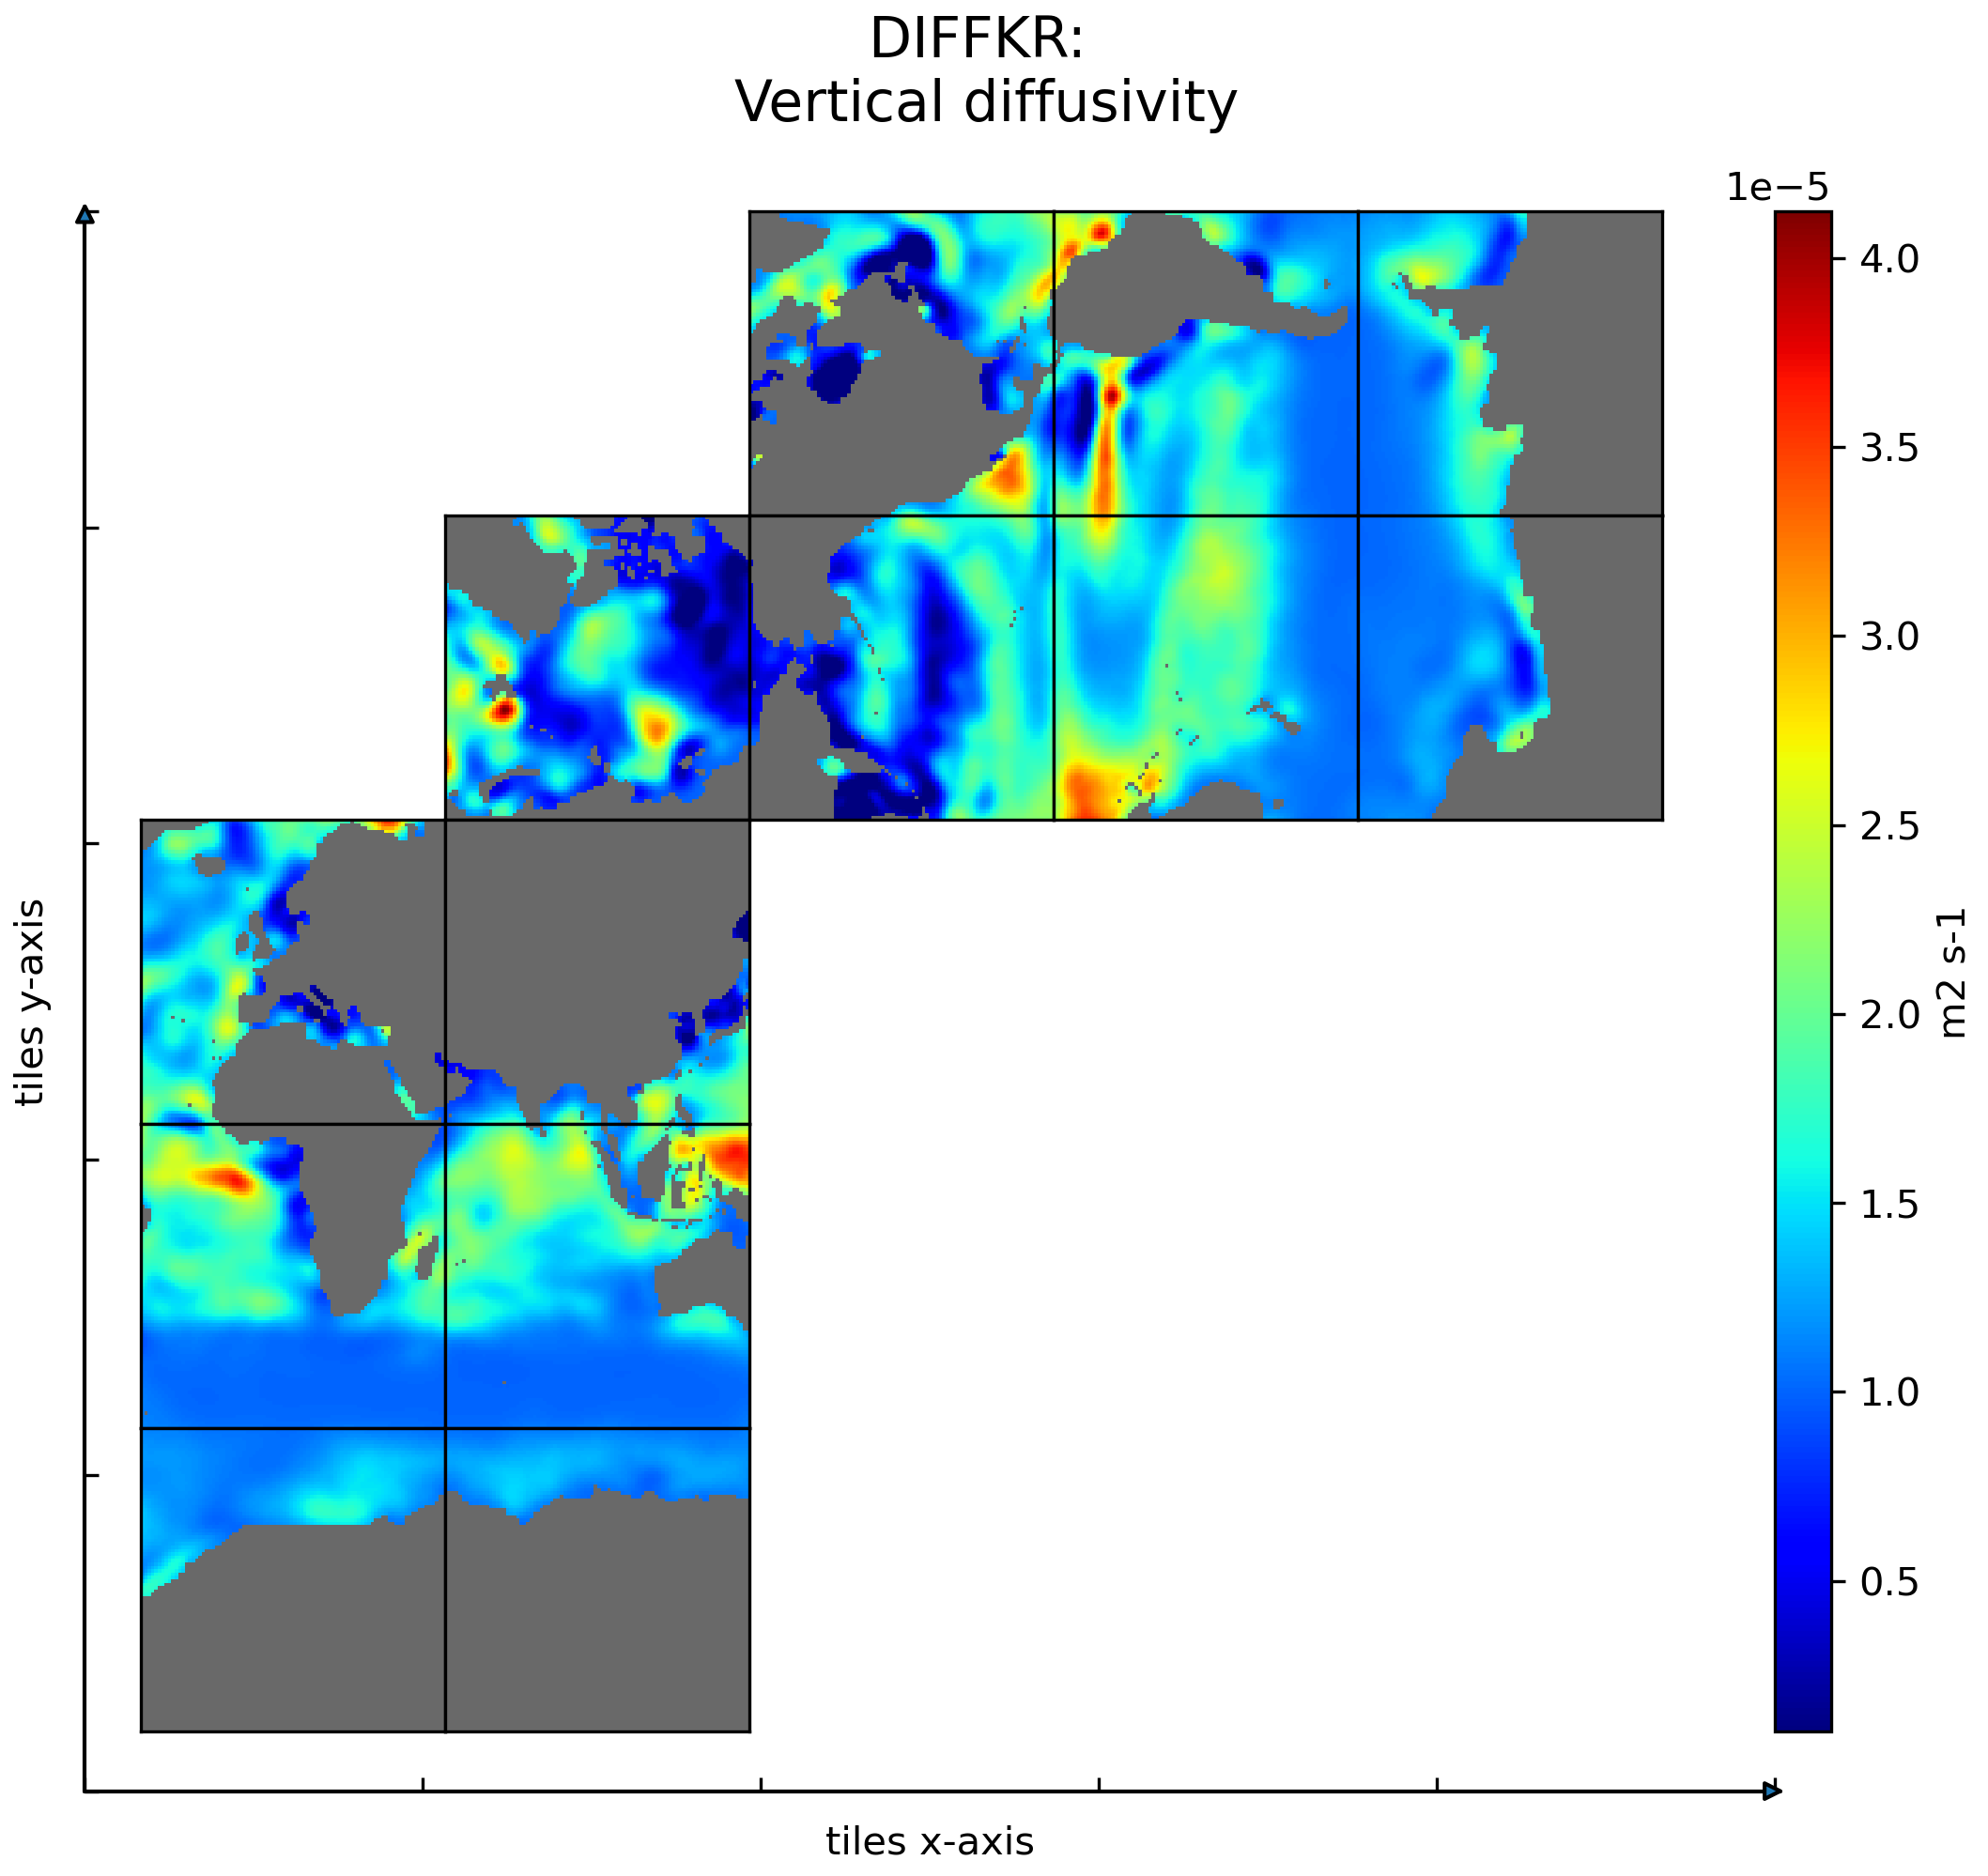
\includegraphics[scale=0.5]{../images/plots/native_plots/Ocean_3D_Gent-Mcwilliams_Redi_and_Background_Vertical_Diffusivity_Coefficients_for_the_Lat-Lon-Cap_90_(llc90)_Native_Model_Grid_(Version_4_Release_4)/DIFFKR.png}
\caption{\\Dataset: OCEAN\_3D\_MIXING\_COEFFS\\Variable: DIFFKR}
\label{tab:table-OCEAN_3D_MIXING_COEFFS_DIFFKR-Plot}
\end{figure}
\pagebreak
\subsubsection{Native Variable KAPGM}
\begin{longtable}{|p{0.06\textwidth}|p{0.41\textwidth}|p{0.39\textwidth}|p{0.06\textwidth}|}
\caption{CDL description of OCEAN\_3D\_MIXING\_COEFFS's KAPGM variable}
\label{tab:table-OCEAN_3D_MIXING_COEFFS_KAPGM} \\ 
\hline \endhead \hline \endfoot
\rowcolor{lightgray} \textbf{Storage Type} & \textbf{Variable Name} & \textbf{Description} & \textbf{Unit} \\ \hline
float32 & KAPGM & Gent-McWilliams diffusivity & m2 s-1 \\ \hline
\rowcolor{lightgray}  \multicolumn{4}{|p{1.00\textwidth}|}{\textbf{CDL Description}} \\ \hline
\multicolumn{4}{|p{1.00\textwidth}|}{\makecell{\parbox{1\textwidth}{float32 KAPGM(k, tile, j, i)\\
\hspace*{0.5cm}KAPGM: \_FillValue = 9.96921e+36\\
\hspace*{0.5cm}KAPGM: coverage\_content\_type = modelResult\\
\hspace*{0.5cm}KAPGM: long\_name = Gent: McWilliams diffusivity\\
\hspace*{0.5cm}KAPGM: units = m2 s: 1\\
\hspace*{0.5cm}KAPGM: valid\_min = 100.0\\
\hspace*{0.5cm}KAPGM: valid\_max = 10000.0\\
\hspace*{0.5cm}KAPGM: coordinates = Z XC YC}}} \\ \hline
\rowcolor{lightgray} \multicolumn{4}{|p{1.00\textwidth}|}{\textbf{Comments}} \\ \hline
\multicolumn{4}{|p{1\textwidth}|}{Gent-McWilliams diffusivity coefficient as described in Gent and McWilliams (1990, JPO). Note: KAPGM is a model control variable and has been optimized from a spatially invariant first guess of 1e3 m2 s-1.} \\ \hline
\end{longtable}

\begin{figure}[H]
\centering
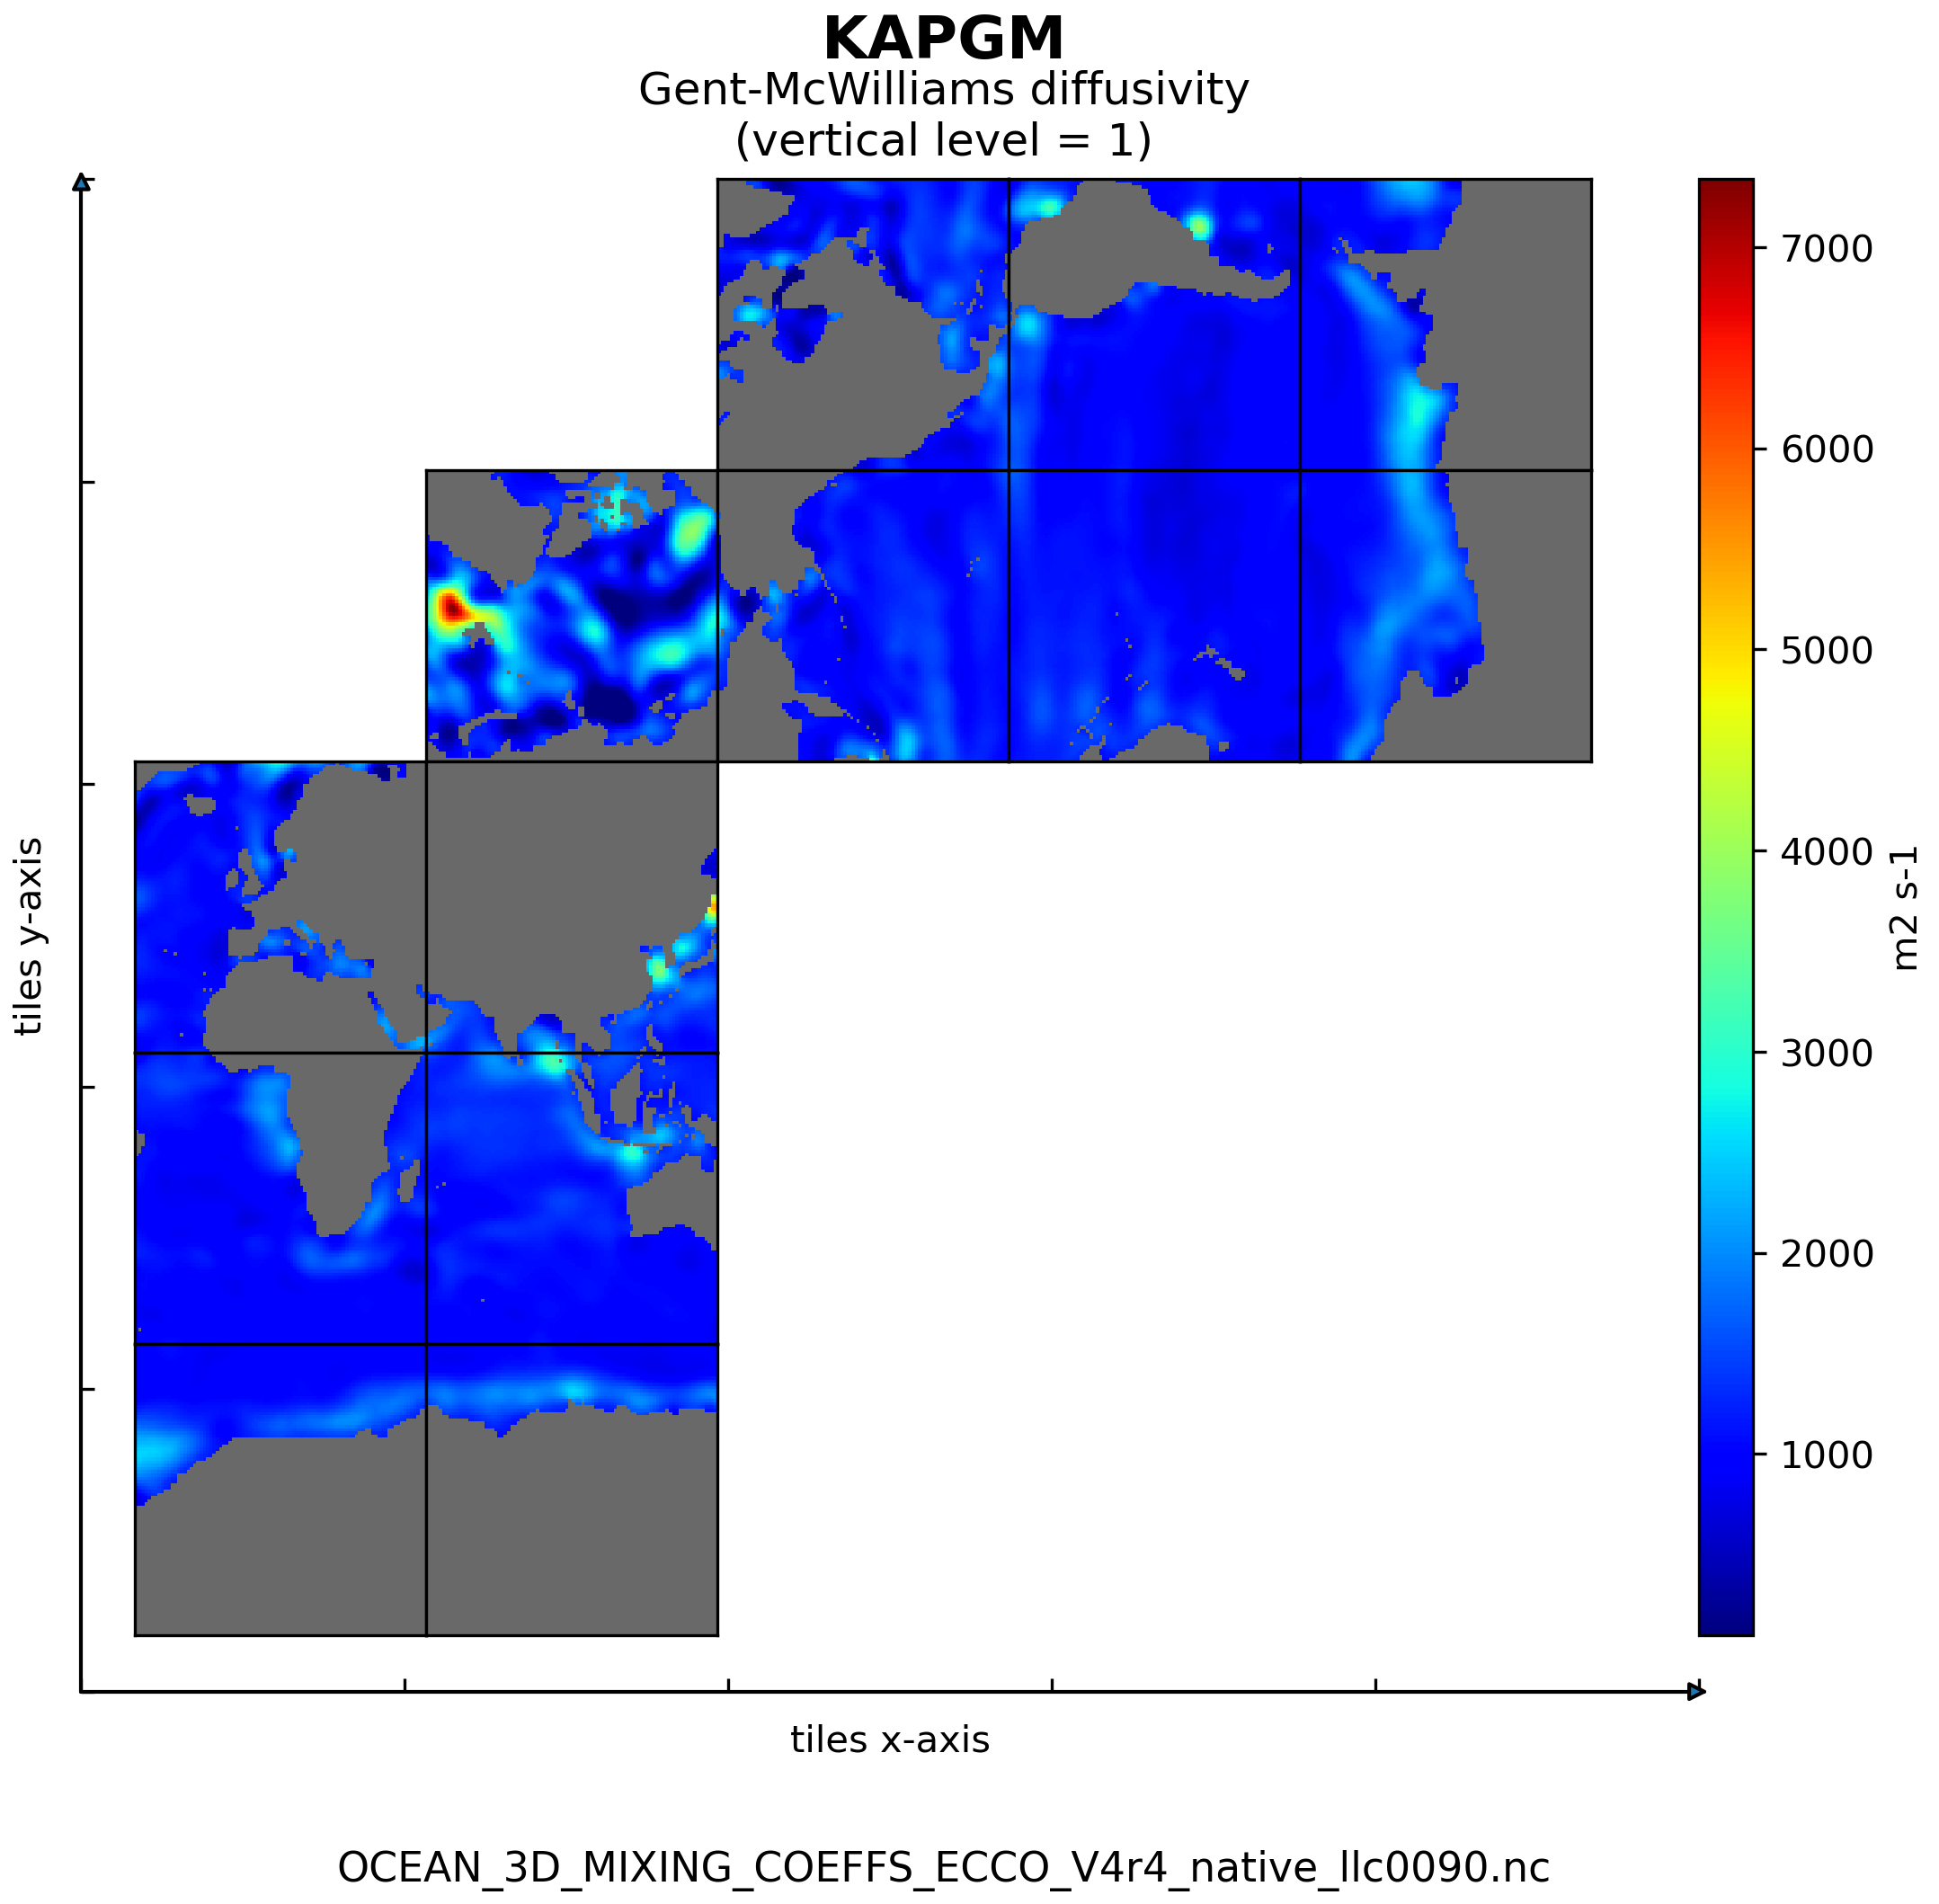
\includegraphics[scale=0.5]{../images/plots/native_plots/Ocean_3D_Gent-Mcwilliams_Redi_and_Background_Vertical_Diffusivity_Coefficients_for_the_Lat-Lon-Cap_90_(llc90)_Native_Model_Grid_(Version_4_Release_4)/KAPGM.png}
\caption{\\Dataset: OCEAN\_3D\_MIXING\_COEFFS\\Variable: KAPGM}
\label{tab:table-OCEAN_3D_MIXING_COEFFS_KAPGM-Plot}
\end{figure}
\pagebreak
\subsubsection{Native Variable KAPREDI}
\begin{longtable}{|p{0.06\textwidth}|p{0.41\textwidth}|p{0.39\textwidth}|p{0.06\textwidth}|}
\caption{CDL description of OCEAN\_3D\_MIXING\_COEFFS's KAPREDI variable}
\label{tab:table-OCEAN_3D_MIXING_COEFFS_KAPREDI} \\ 
\hline \endhead \hline \endfoot
\rowcolor{lightgray} \textbf{Storage Type} & \textbf{Variable Name} & \textbf{Description} & \textbf{Unit} \\ \hline
float32 & KAPREDI & Along-isopycnal diffusivity & m2 s-1 \\ \hline
\rowcolor{lightgray}  \multicolumn{4}{|p{1.00\textwidth}|}{\textbf{CDL Description}} \\ \hline
\multicolumn{4}{|p{1.00\textwidth}|}{\makecell{\parbox{1\textwidth}{float32 KAPREDI(k, tile, j, i)\\
\hspace*{0.5cm}KAPREDI: \_FillValue = 9.96921e+36\\
\hspace*{0.5cm}KAPREDI: coverage\_content\_type = modelResult\\
\hspace*{0.5cm}KAPREDI: long\_name = Along: isopycnal diffusivity\\
\hspace*{0.5cm}KAPREDI: units = m2 s: 1\\
\hspace*{0.5cm}KAPREDI: valid\_min = 100.0\\
\hspace*{0.5cm}KAPREDI: valid\_max = 10000.0\\
\hspace*{0.5cm}KAPREDI: coordinates = Z XC YC}}} \\ \hline
\rowcolor{lightgray} \multicolumn{4}{|p{1.00\textwidth}|}{\textbf{Comments}} \\ \hline
\multicolumn{4}{|p{1\textwidth}|}{Redi along-isopycnal diffusivity coefficient as described in Redi (1982, JPO). Note: KAPREDI is a model control variable and has been optimized from a spatially invariant first guess of 1e3 m2 s-1.} \\ \hline
\end{longtable}

\begin{figure}[H]
\centering
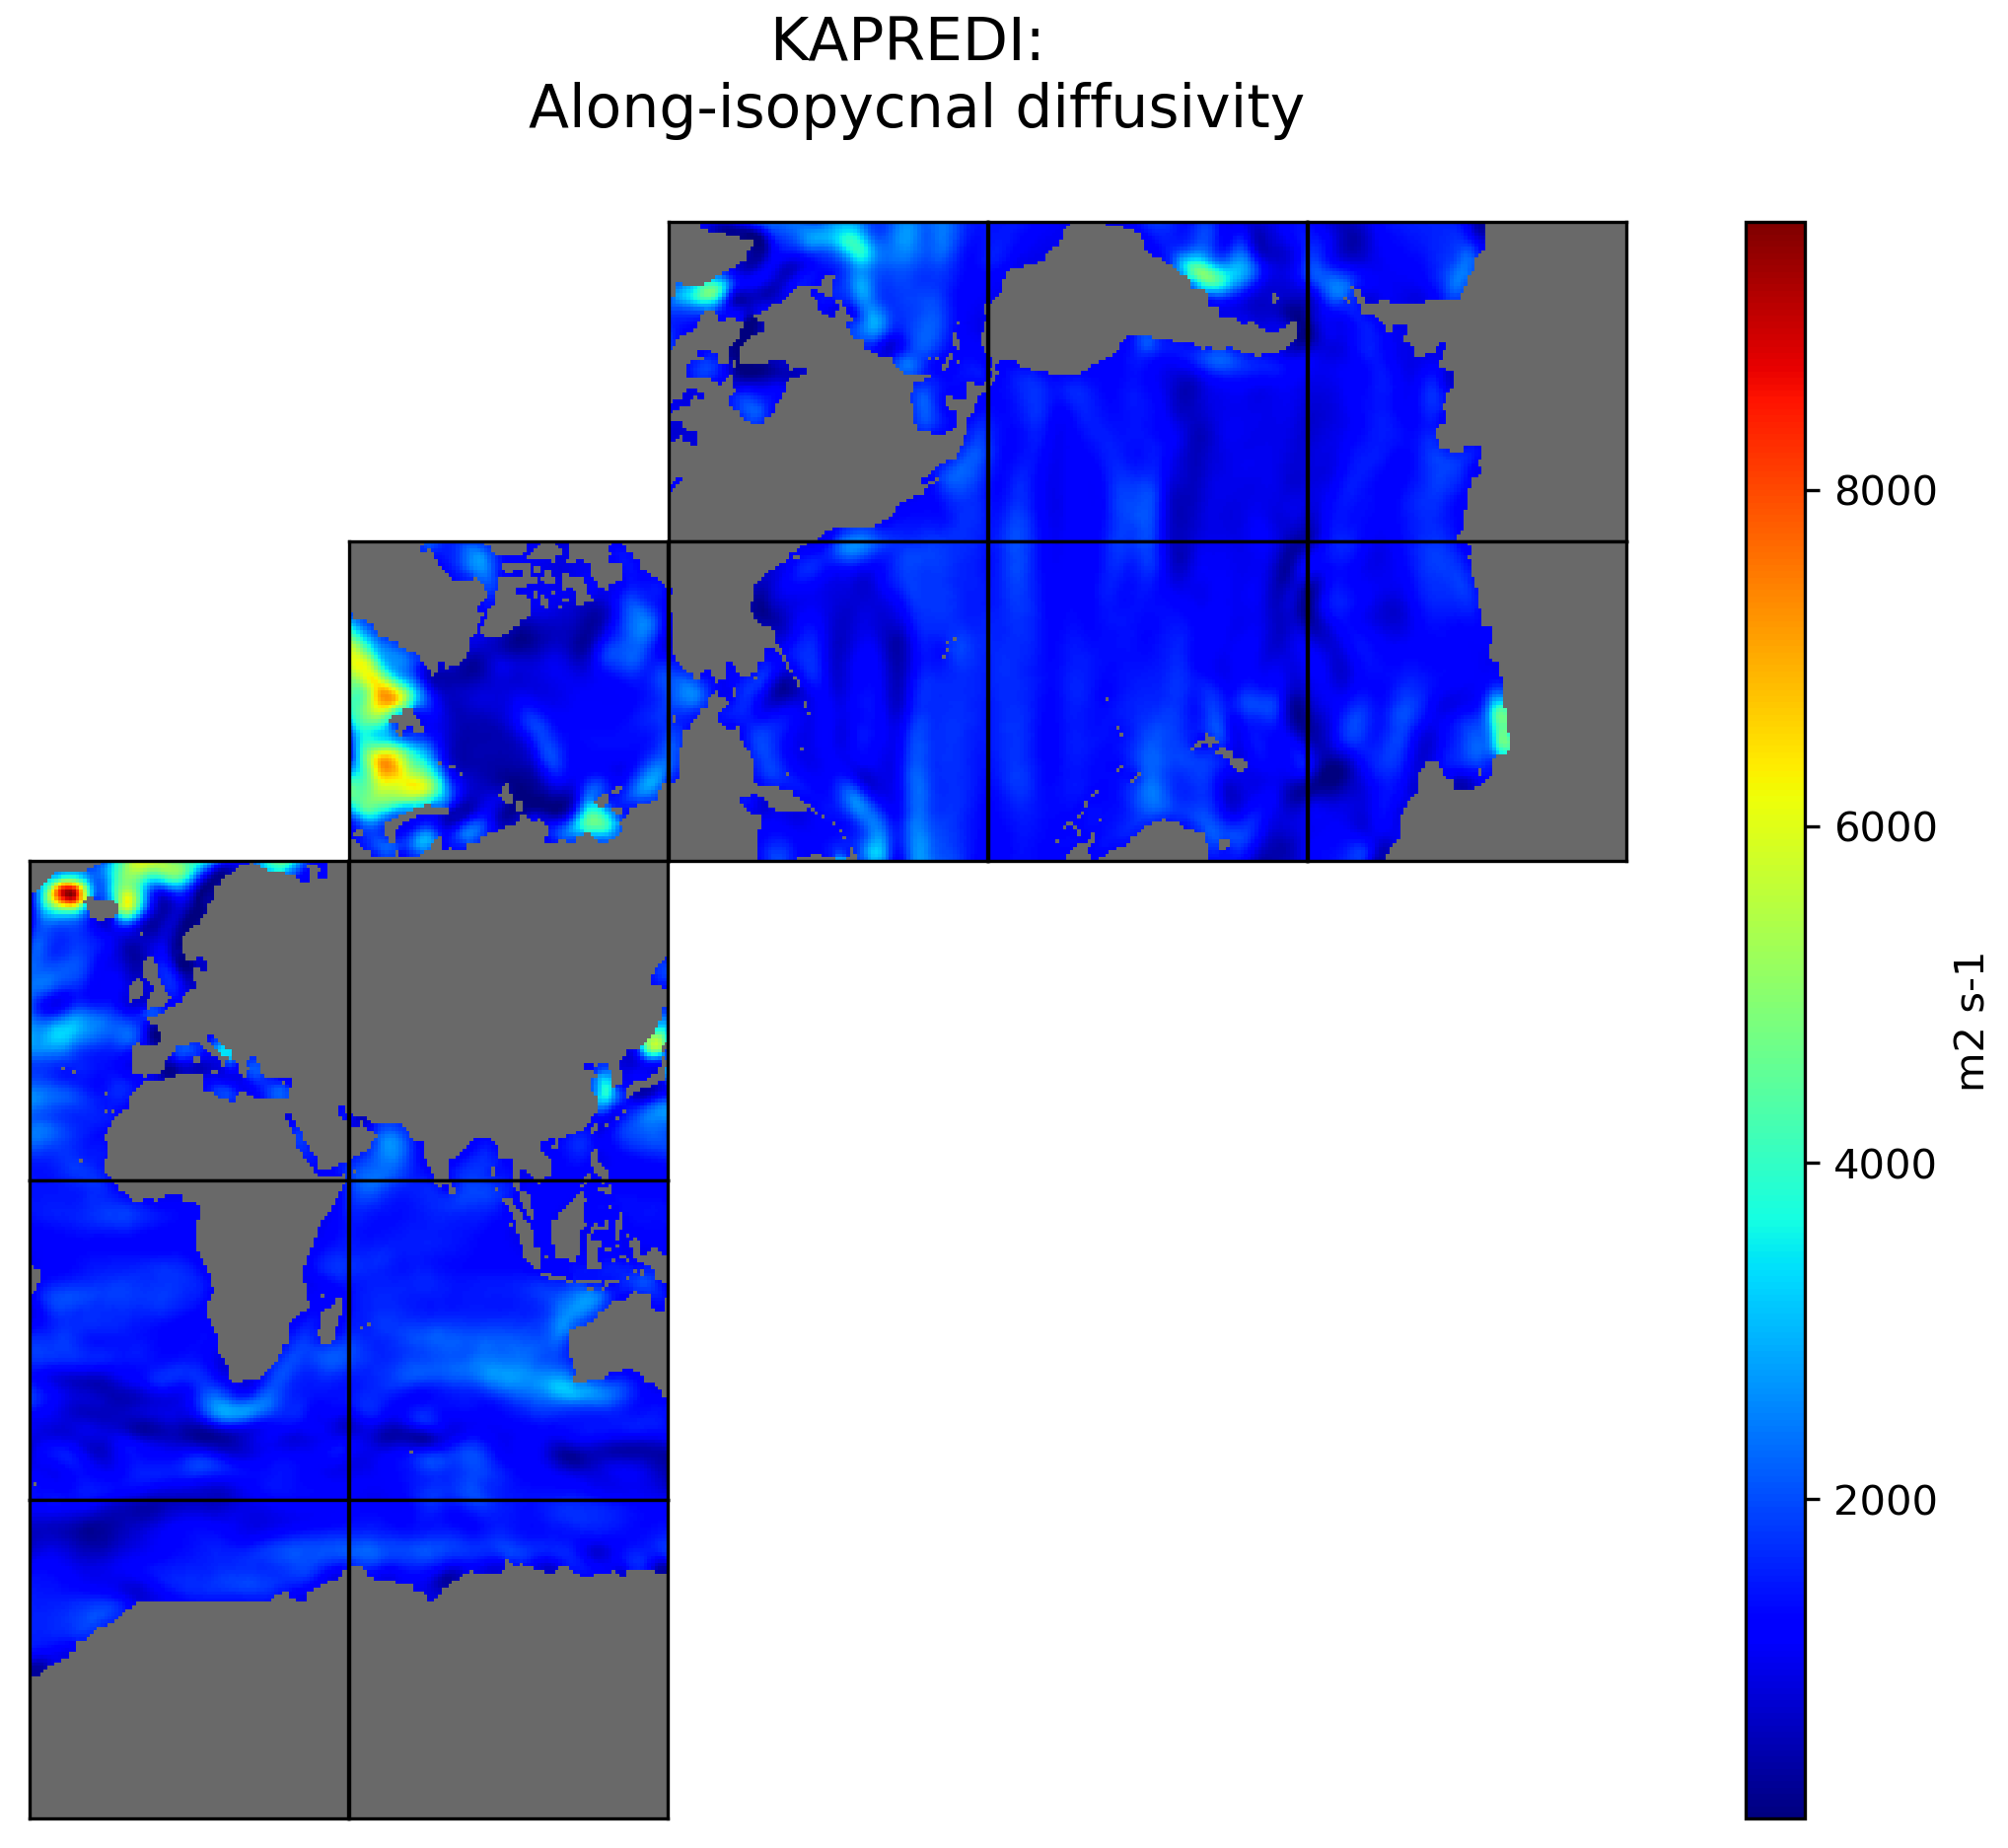
\includegraphics[scale=0.5]{../images/plots/native_plots/Ocean_3D_Gent-Mcwilliams_Redi_and_Background_Vertical_Diffusivity_Coefficients_for_the_Lat-Lon-Cap_90_(llc90)_Native_Model_Grid_(Version_4_Release_4)/KAPREDI.png}
\caption{\\Dataset: OCEAN\_3D\_MIXING\_COEFFS\\Variable: KAPREDI}
\label{tab:table-OCEAN_3D_MIXING_COEFFS_KAPREDI-Plot}
\end{figure}
\pagebreak
\subsection{Native NetCDF OCEAN\_3D\_MOMENTUM\_TEND}
\newp
\begin{longtable}{|p{0.1\textwidth}|p{0.5\textwidth}|}
\caption{Variables in the dataset OCEAN\_3D\_MOMENTUM\_TEND}
\label{tab:table-OCEAN_3D_MOMENTUM_TEND-fields} \\ 
\hline \endhead \hline \endfoot
\rowcolor{lightgray} \textbf{Dataset:} & \textbf{OCEAN\_3D\_MOMENTUM\_TEND} \\ \hline
Field: &Um\_dPHdx \\ \hline
Field: &Vm\_dPHdy \\ \hline
\end{longtable}

\pagebreak
\subsubsection{Native Variable Um\_dPHdx}
\begin{longtable}{|p{0.06\textwidth}|p{0.41\textwidth}|p{0.39\textwidth}|p{0.06\textwidth}|}
\caption{CDL description of OCEAN\_3D\_MOMENTUM\_TEND's Um\_dPHdx variable}
\label{tab:table-OCEAN_3D_MOMENTUM_TEND_Um_dPHdx} \\ 
\hline \endhead \hline \endfoot
\rowcolor{lightgray} \textbf{Storage Type} & \textbf{Variable Name} & \textbf{Description} & \textbf{Unit} \\ \hline
float32 & Um\_dPHdx & Momentum tendency in the model +x direction & m s-2 \\ \hline
\rowcolor{lightgray}  \multicolumn{4}{|p{1.00\textwidth}|}{\textbf{CDL Description}} \\ \hline
\multicolumn{4}{|p{1.00\textwidth}|}{\makecell{\parbox{1\textwidth}{float32 Um\_dPHdx(time, k, tile, j, i\_g)\\
\hspace*{0.5cm}Um\_dPHdx: \_FillValue = 9.96921e+36\\
\hspace*{0.5cm}Um\_dPHdx: long\_name = Momentum tendency in the model +x direction\\
\hspace*{0.5cm}Um\_dPHdx: units = m s: 2\\
\hspace*{0.5cm}Um\_dPHdx: mate = Vm\_dPHdy\\
\hspace*{0.5cm}Um\_dPHdx: coverage\_content\_type = modelResult\\
\hspace*{0.5cm}Um\_dPHdx: coordinates = time Z\\
\hspace*{0.5cm}Um\_dPHdx: valid\_min = : 0.0010651482734829187\\
\hspace*{0.5cm}Um\_dPHdx: valid\_max = 0.0011411579325795174}}} \\ \hline
\rowcolor{lightgray} \multicolumn{4}{|p{1.00\textwidth}|}{\textbf{Comments}} \\ \hline
\multicolumn{4}{|p{1\textwidth}|}{Momentum tendency in the +x direction due to the hydrostatic pressure gradient at the 'u' face of the native model grid cell . Note: the model +x direction does not necessarily correspond to the geographical east-west direction because the x and y axes of the model's curvilinear lat-lon-cap (llc) grid have arbitrary orientations which vary within and across tiles.} \\ \hline
\end{longtable}

\begin{figure}[H]
\centering
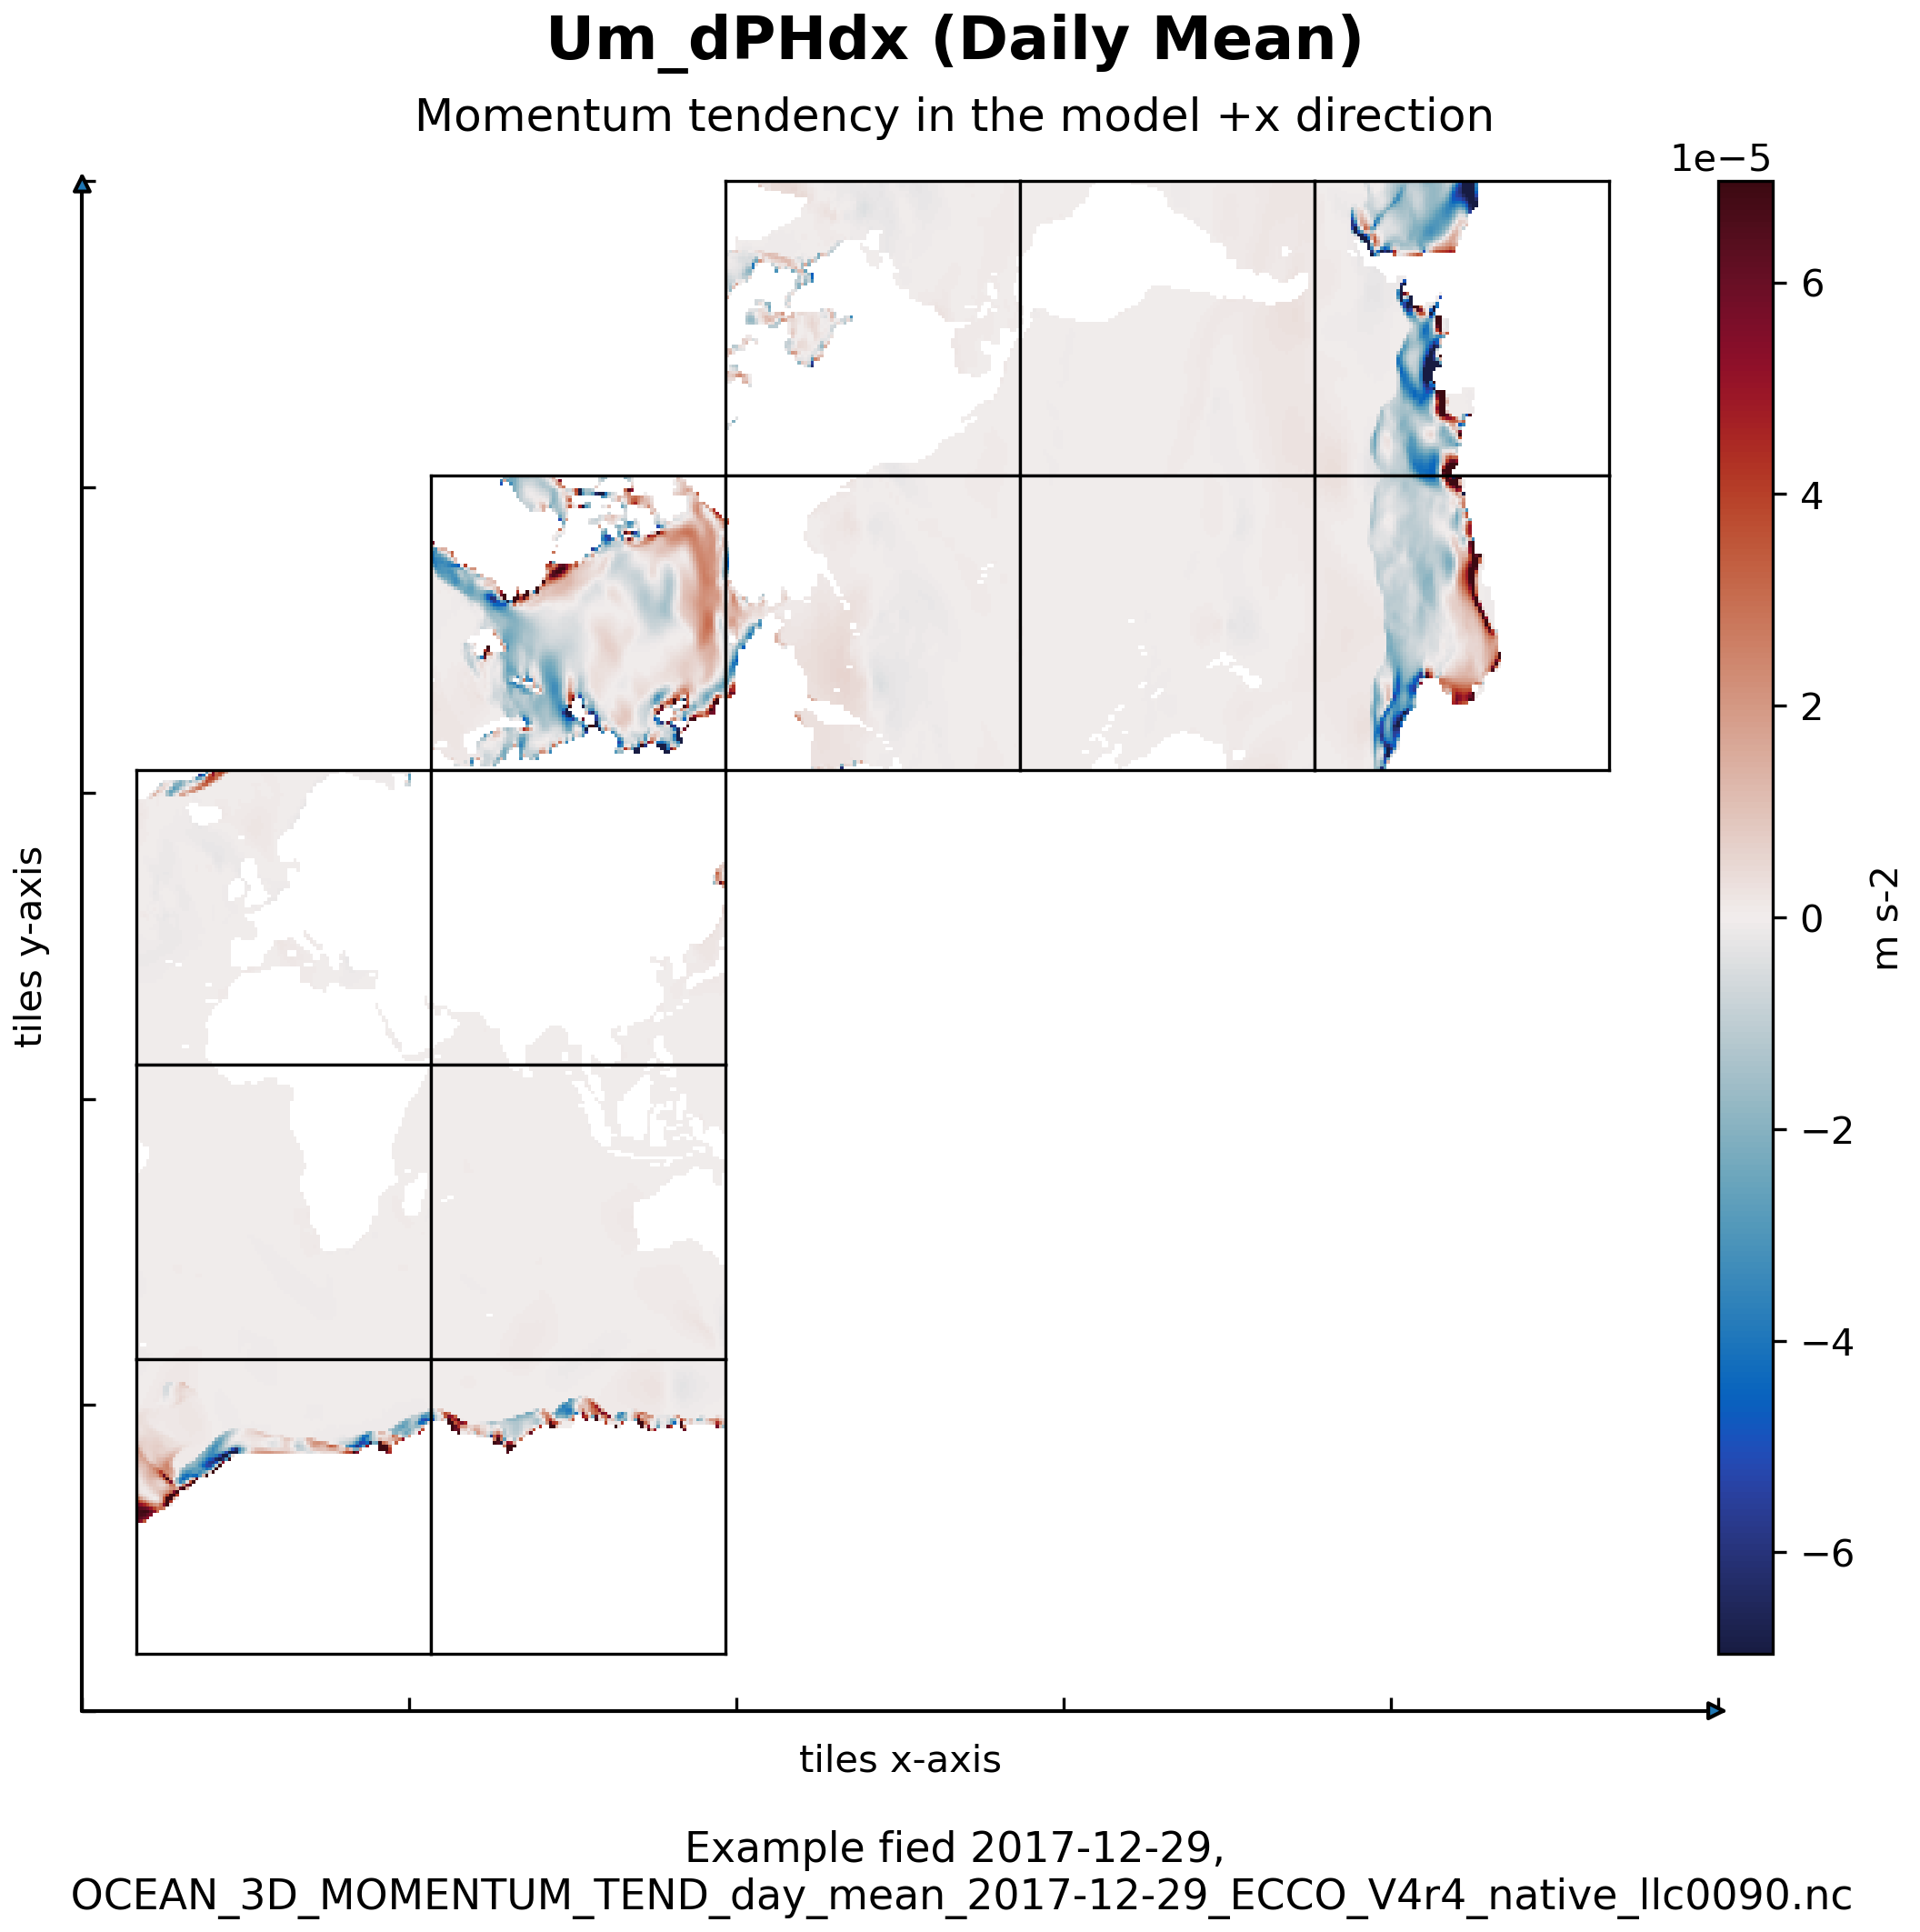
\includegraphics[scale=0.5]{../images/plots/native_plots/Ocean_Three-Dimensional_Momentum_Tendency/Um_dPHdx.png}
\caption{\\Dataset: OCEAN\_3D\_MOMENTUM\_TEND\\Variable: Um\_dPHdx}
\label{tab:table-OCEAN_3D_MOMENTUM_TEND_Um_dPHdx-Plot}
\end{figure}
\pagebreak
\subsubsection{Native Variable Vm\_dPHdy}
\begin{longtable}{|p{0.06\textwidth}|p{0.41\textwidth}|p{0.39\textwidth}|p{0.06\textwidth}|}
\caption{CDL description of OCEAN\_3D\_MOMENTUM\_TEND's Vm\_dPHdy variable}
\label{tab:table-OCEAN_3D_MOMENTUM_TEND_Vm_dPHdy} \\ 
\hline \endhead \hline \endfoot
\rowcolor{lightgray} \textbf{Storage Type} & \textbf{Variable Name} & \textbf{Description} & \textbf{Unit} \\ \hline
float32 & Vm\_dPHdy & Momentum tendency in the model +y direction & m s-2 \\ \hline
\rowcolor{lightgray}  \multicolumn{4}{|p{1.00\textwidth}|}{\textbf{CDL Description}} \\ \hline
\multicolumn{4}{|p{1.00\textwidth}|}{\makecell{\parbox{1\textwidth}{float32 Vm\_dPHdy(time, k, tile, j\_g, i)\\
\hspace*{0.5cm}Vm\_dPHdy: \_FillValue = 9.96921e+36\\
\hspace*{0.5cm}Vm\_dPHdy: long\_name = Momentum tendency in the model +y direction\\
\hspace*{0.5cm}Vm\_dPHdy: units = m s: 2\\
\hspace*{0.5cm}Vm\_dPHdy: mate = Um\_dPHdx\\
\hspace*{0.5cm}Vm\_dPHdy: coverage\_content\_type = modelResult\\
\hspace*{0.5cm}Vm\_dPHdy: coordinates = time Z\\
\hspace*{0.5cm}Vm\_dPHdy: valid\_min = : 0.0015932790702208877\\
\hspace*{0.5cm}Vm\_dPHdy: valid\_max = 0.0008858146029524505}}} \\ \hline
\rowcolor{lightgray} \multicolumn{4}{|p{1.00\textwidth}|}{\textbf{Comments}} \\ \hline
\multicolumn{4}{|p{1\textwidth}|}{Momentum tendency in the +y direction due to the hydrostatic pressure gradient at the 'v' face of the native model grid cell . Note: the model +y direction does not necessarily correspond to the geographical north-south direction because the x and y axes of the model's curvilinear lat-lon-cap (llc) grid have arbitrary orientations which vary within and across tiles.} \\ \hline
\end{longtable}

\begin{figure}[H]
\centering
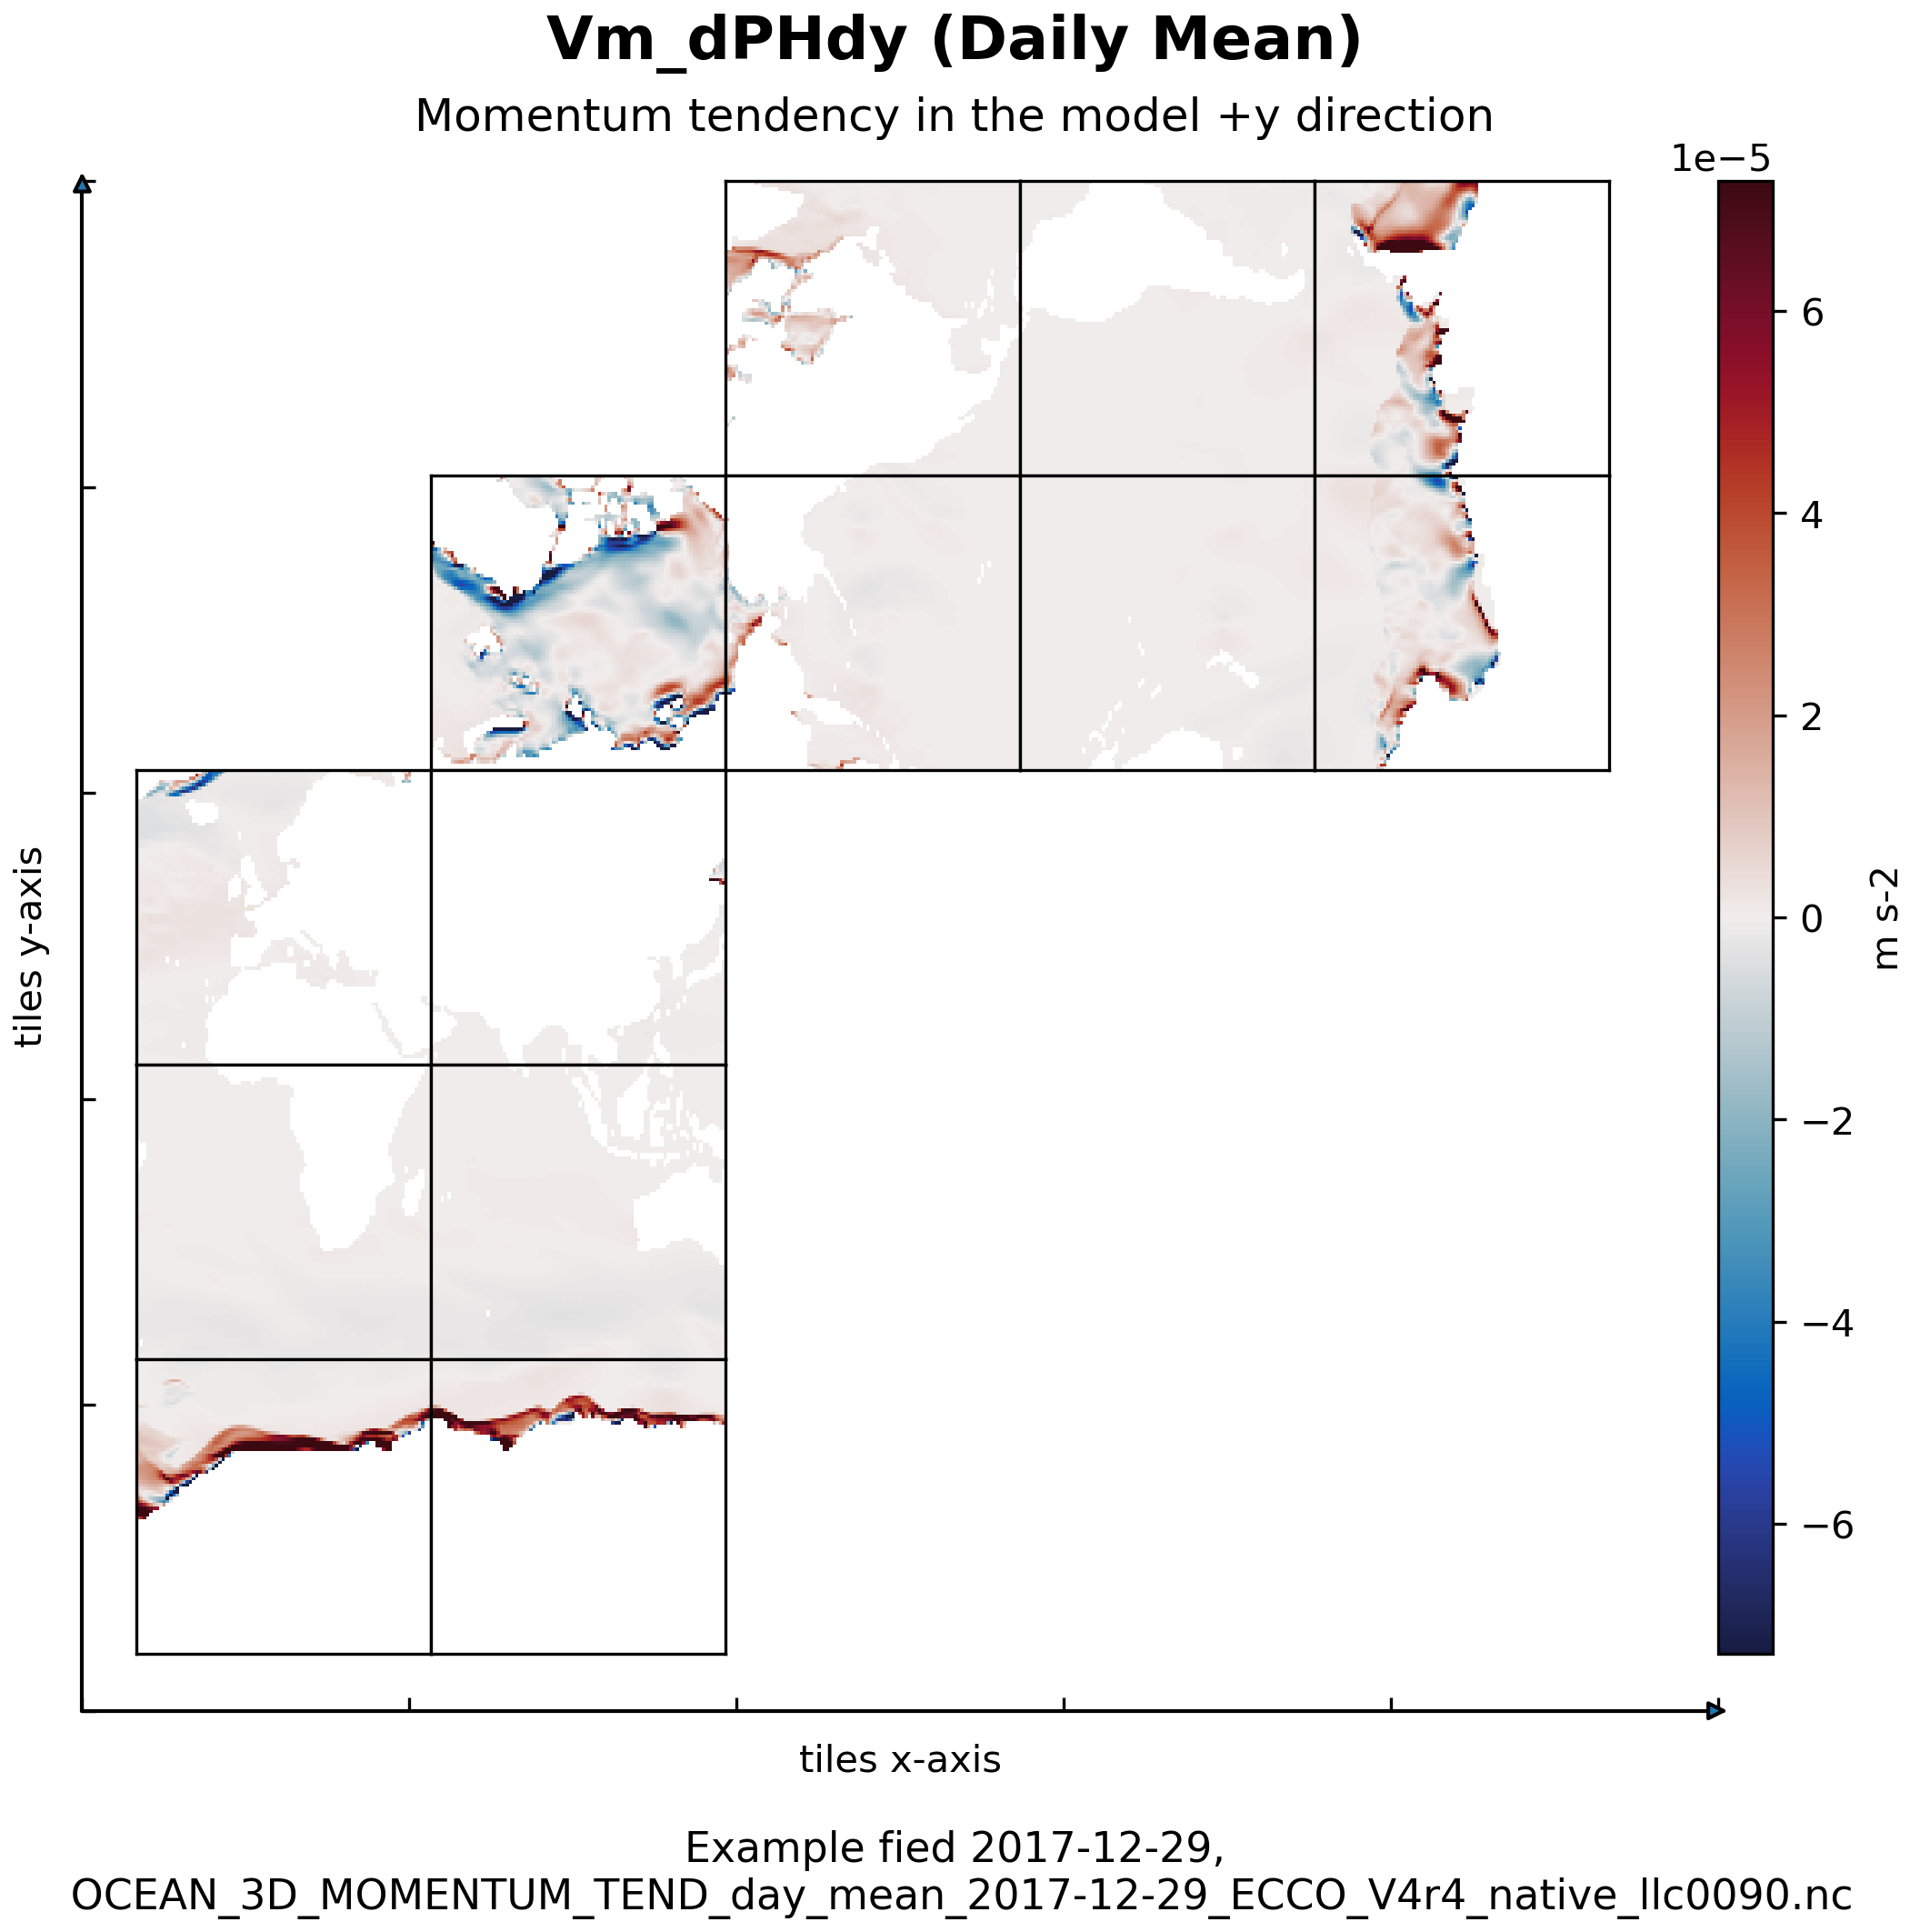
\includegraphics[scale=0.5]{../images/plots/native_plots/Ocean_Three-Dimensional_Momentum_Tendency/Vm_dPHdy.png}
\caption{\\Dataset: OCEAN\_3D\_MOMENTUM\_TEND\\Variable: Vm\_dPHdy}
\label{tab:table-OCEAN_3D_MOMENTUM_TEND_Vm_dPHdy-Plot}
\end{figure}
\pagebreak
\subsection{Native NetCDF OCEAN\_3D\_SALINITY\_FLUX}
\newp
\begin{longtable}{|p{0.1\textwidth}|p{0.5\textwidth}|}
\caption{Variables in the dataset OCEAN\_3D\_SALINITY\_FLUX}
\label{tab:table-OCEAN_3D_SALINITY_FLUX-fields} \\ 
\hline \endhead \hline \endfoot
\rowcolor{lightgray} \textbf{Dataset:} & \textbf{OCEAN\_3D\_SALINITY\_FLUX} \\ \hline
Field: &ADVx\_SLT \\ \hline
Field: &DFxE\_SLT \\ \hline
Field: &ADVy\_SLT \\ \hline
Field: &DFyE\_SLT \\ \hline
Field: &ADVr\_SLT \\ \hline
Field: &DFrE\_SLT \\ \hline
Field: &DFrI\_SLT \\ \hline
Field: &oceSPtnd \\ \hline
\end{longtable}

\pagebreak
\subsubsection{Native Variable ADVr\_SLT}
\begin{longtable}{|p{0.06\textwidth}|p{0.41\textwidth}|p{0.39\textwidth}|p{0.06\textwidth}|}
\caption{CDL description of OCEAN\_3D\_SALINITY\_FLUX's ADVr\_SLT variable}
\label{tab:table-OCEAN_3D_SALINITY_FLUX_ADVr_SLT} \\ 
\hline \endhead \hline \endfoot
\rowcolor{lightgray} \textbf{Storage Type} & \textbf{Variable Name} & \textbf{Description} & \textbf{Unit} \\ \hline
float32 & ADVr\_SLT & Vertical advective flux of salinity & 1e-3 m3 s-1 \\ \hline
\rowcolor{lightgray}  \multicolumn{4}{|p{1.00\textwidth}|}{\textbf{CDL Description}} \\ \hline
\multicolumn{4}{|p{1.00\textwidth}|}{\makecell{\parbox{1\textwidth}{float32 ADVr\_SLT(time, k\_l, tile, j, i)\\
\hspace*{0.5cm}ADVr\_SLT: \_FillValue = 9.96921e+36\\
\hspace*{0.5cm}ADVr\_SLT: long\_name = Vertical advective flux of salinity\\
\hspace*{0.5cm}ADVr\_SLT: units = 1e: 3 m3 s: 1\\
\hspace*{0.5cm}ADVr\_SLT: coverage\_content\_type = modelResult\\
\hspace*{0.5cm}ADVr\_SLT: direction = >0 decreases salinity (SALT)\\
\hspace*{0.5cm}ADVr\_SLT: coordinates = XC Zl YC time\\
\hspace*{0.5cm}ADVr\_SLT: valid\_min = : 324149856.0\\
\hspace*{0.5cm}ADVr\_SLT: valid\_max = 263294624.0}}} \\ \hline
\rowcolor{lightgray} \multicolumn{4}{|p{1.00\textwidth}|}{\textbf{Comments}} \\ \hline
\multicolumn{4}{|p{1\textwidth}|}{Vertical advective flux of salinity (SALT) in the +z direction through the top 'w' face of the tracer cell on the native model grid. Note: in the Arakawa-C grid, vertical flux quantities are staggered relative to the tracer cells with indexing such that +ADVr\_SLT(i,j,k\_l) corresponds to upward +z fluxes through the top 'w' face of the tracer cell at (i,j,k). Salinity defined using CF convention 'Sea water salinity is the salt content of sea water, often on the Practical Salinity Scale of 1978. However, the unqualified term 'salinity' is generic and does not necessarily imply any particular method of calculation. The units of salinity are dimensionless and the units attribute should normally be given as 1e-3 or 0.001 i.e. parts per thousand.' see https://cfconventions.org/Data/cf-standard-names/73/build/cf-standard-name-table.html} \\ \hline
\end{longtable}

\begin{figure}[H]
\centering
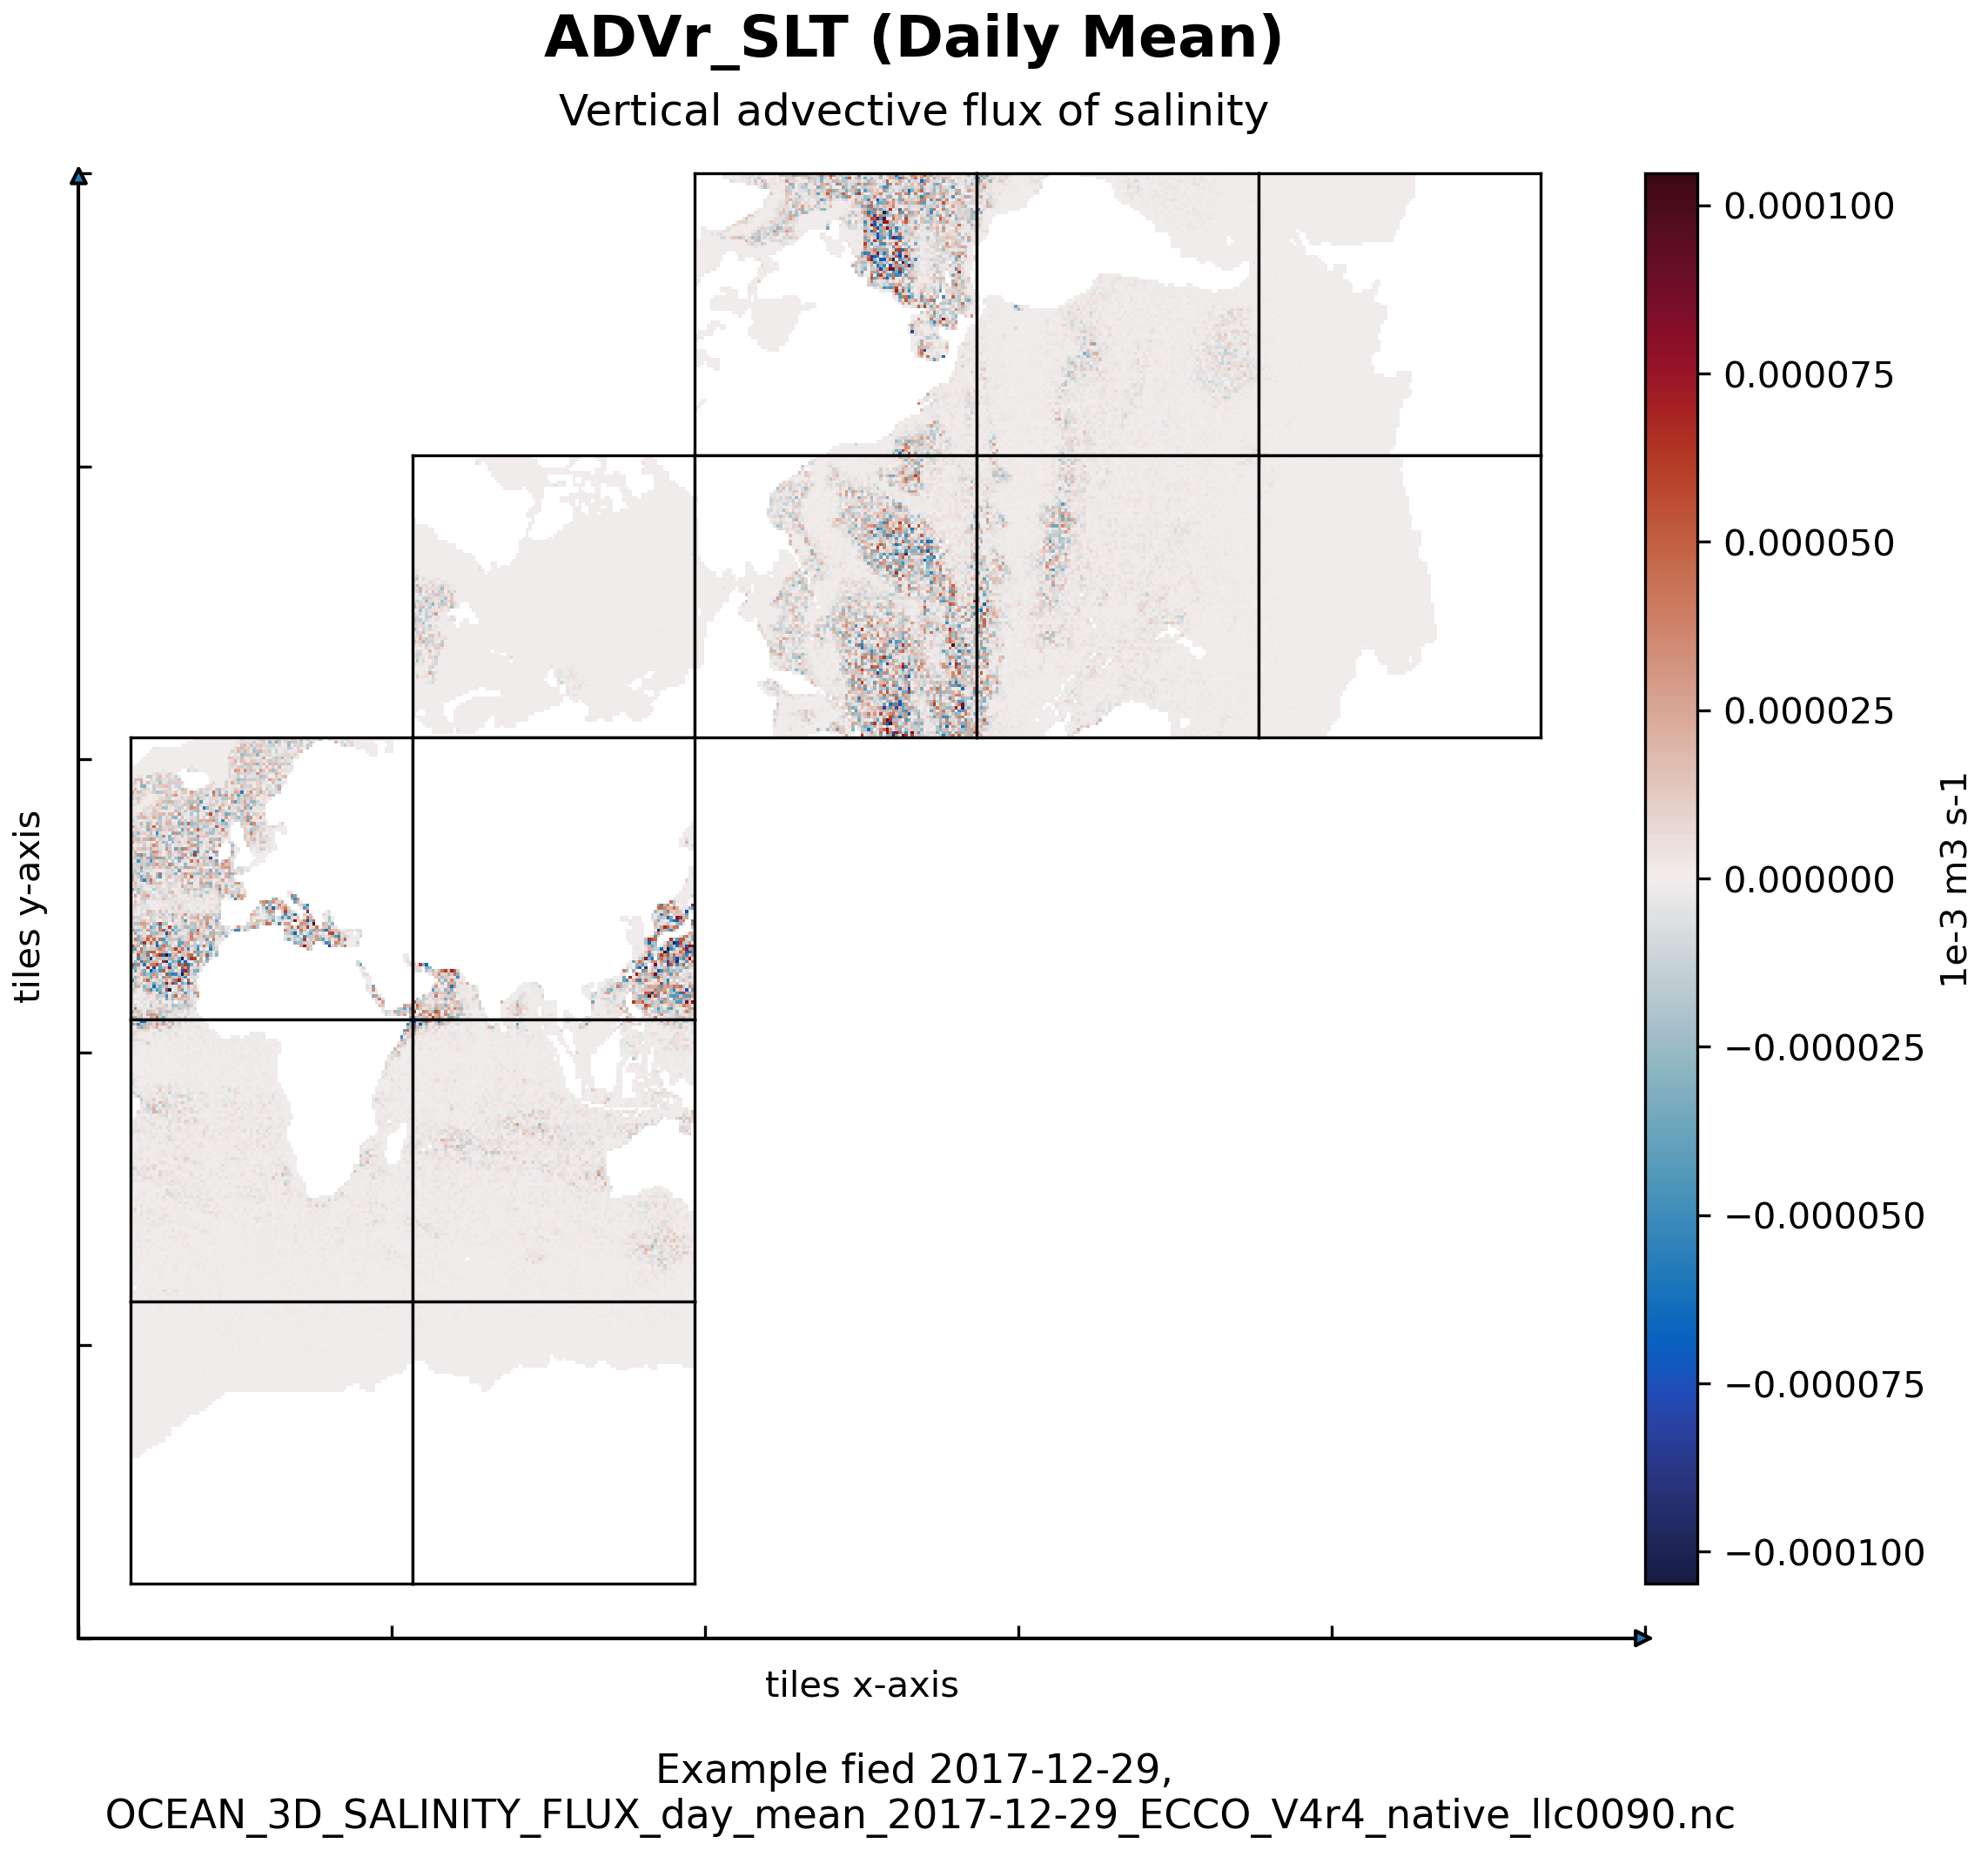
\includegraphics[scale=0.5]{../images/plots/native_plots/Ocean_Three-Dimensional_Salinity_Fluxes/ADVr_SLT.png}
\caption{\\Dataset: OCEAN\_3D\_SALINITY\_FLUX\\Variable: ADVr\_SLT}
\label{tab:table-OCEAN_3D_SALINITY_FLUX_ADVr_SLT-Plot}
\end{figure}
\pagebreak
\subsubsection{Native Variable ADVx\_SLT}
\begin{longtable}{|p{0.06\textwidth}|p{0.41\textwidth}|p{0.39\textwidth}|p{0.06\textwidth}|}
\caption{CDL description of OCEAN\_3D\_SALINITY\_FLUX's ADVx\_SLT variable}
\label{tab:table-OCEAN_3D_SALINITY_FLUX_ADVx_SLT} \\ 
\hline \endhead \hline \endfoot
\rowcolor{lightgray} \textbf{Storage Type} & \textbf{Variable Name} & \textbf{Description} & \textbf{Unit} \\ \hline
float32 & ADVx\_SLT & Lateral advective flux of salinity in the model +x direction & 1e-3 m3 s-1 \\ \hline
\rowcolor{lightgray}  \multicolumn{4}{|p{1.00\textwidth}|}{\textbf{CDL Description}} \\ \hline
\multicolumn{4}{|p{1.00\textwidth}|}{\makecell{\parbox{1\textwidth}{float32 ADVx\_SLT(time, k, tile, j, i\_g)\\
\hspace*{0.5cm}ADVx\_SLT: \_FillValue = 9.96921e+36\\
\hspace*{0.5cm}ADVx\_SLT: long\_name = Lateral advective flux of salinity in the model +x direction\\
\hspace*{0.5cm}ADVx\_SLT: units = 1e: 3 m3 s: 1\\
\hspace*{0.5cm}ADVx\_SLT: mate = ADVy\_SLT\\
\hspace*{0.5cm}ADVx\_SLT: coverage\_content\_type = modelResult\\
\hspace*{0.5cm}ADVx\_SLT: direction = >0 increases salinity (SALT)\\
\hspace*{0.5cm}ADVx\_SLT: coordinates = Z time\\
\hspace*{0.5cm}ADVx\_SLT: valid\_min = : 181830224.0\\
\hspace*{0.5cm}ADVx\_SLT: valid\_max = 260411296.0}}} \\ \hline
\rowcolor{lightgray} \multicolumn{4}{|p{1.00\textwidth}|}{\textbf{Comments}} \\ \hline
\multicolumn{4}{|p{1\textwidth}|}{Lateral advective flux of salinity (SALT) in the +x direction through the 'u' face of the tracer cell on the native model grid. Note: in the Arakawa-C grid, horizontal flux quantities are staggered relative to the tracer cells with indexing such that +ADVx\_SLT(i\_g,j,k) corresponds to +x fluxes through the 'u' face of the tracer cell at (i,j,k). Also, the model +x direction does not necessarily correspond to the geographical east-west direction because the x and y axes of the model's curvilinear lat-lon-cap (llc) grid have arbitrary orientations which vary within and across tiles. Salinity defined using CF convention 'Sea water salinity is the salt content of sea water, often on the Practical Salinity Scale of 1978. However, the unqualified term 'salinity' is generic and does not necessarily imply any particular method of calculation. The units of salinity are dimensionless and the units attribute should normally be given as 1e-3 or 0.001 i.e. parts per thousand.' see https://cfconventions.org/Data/cf-standard-names/73/build/cf-standard-name-table.html} \\ \hline
\end{longtable}

\begin{figure}[H]
\centering
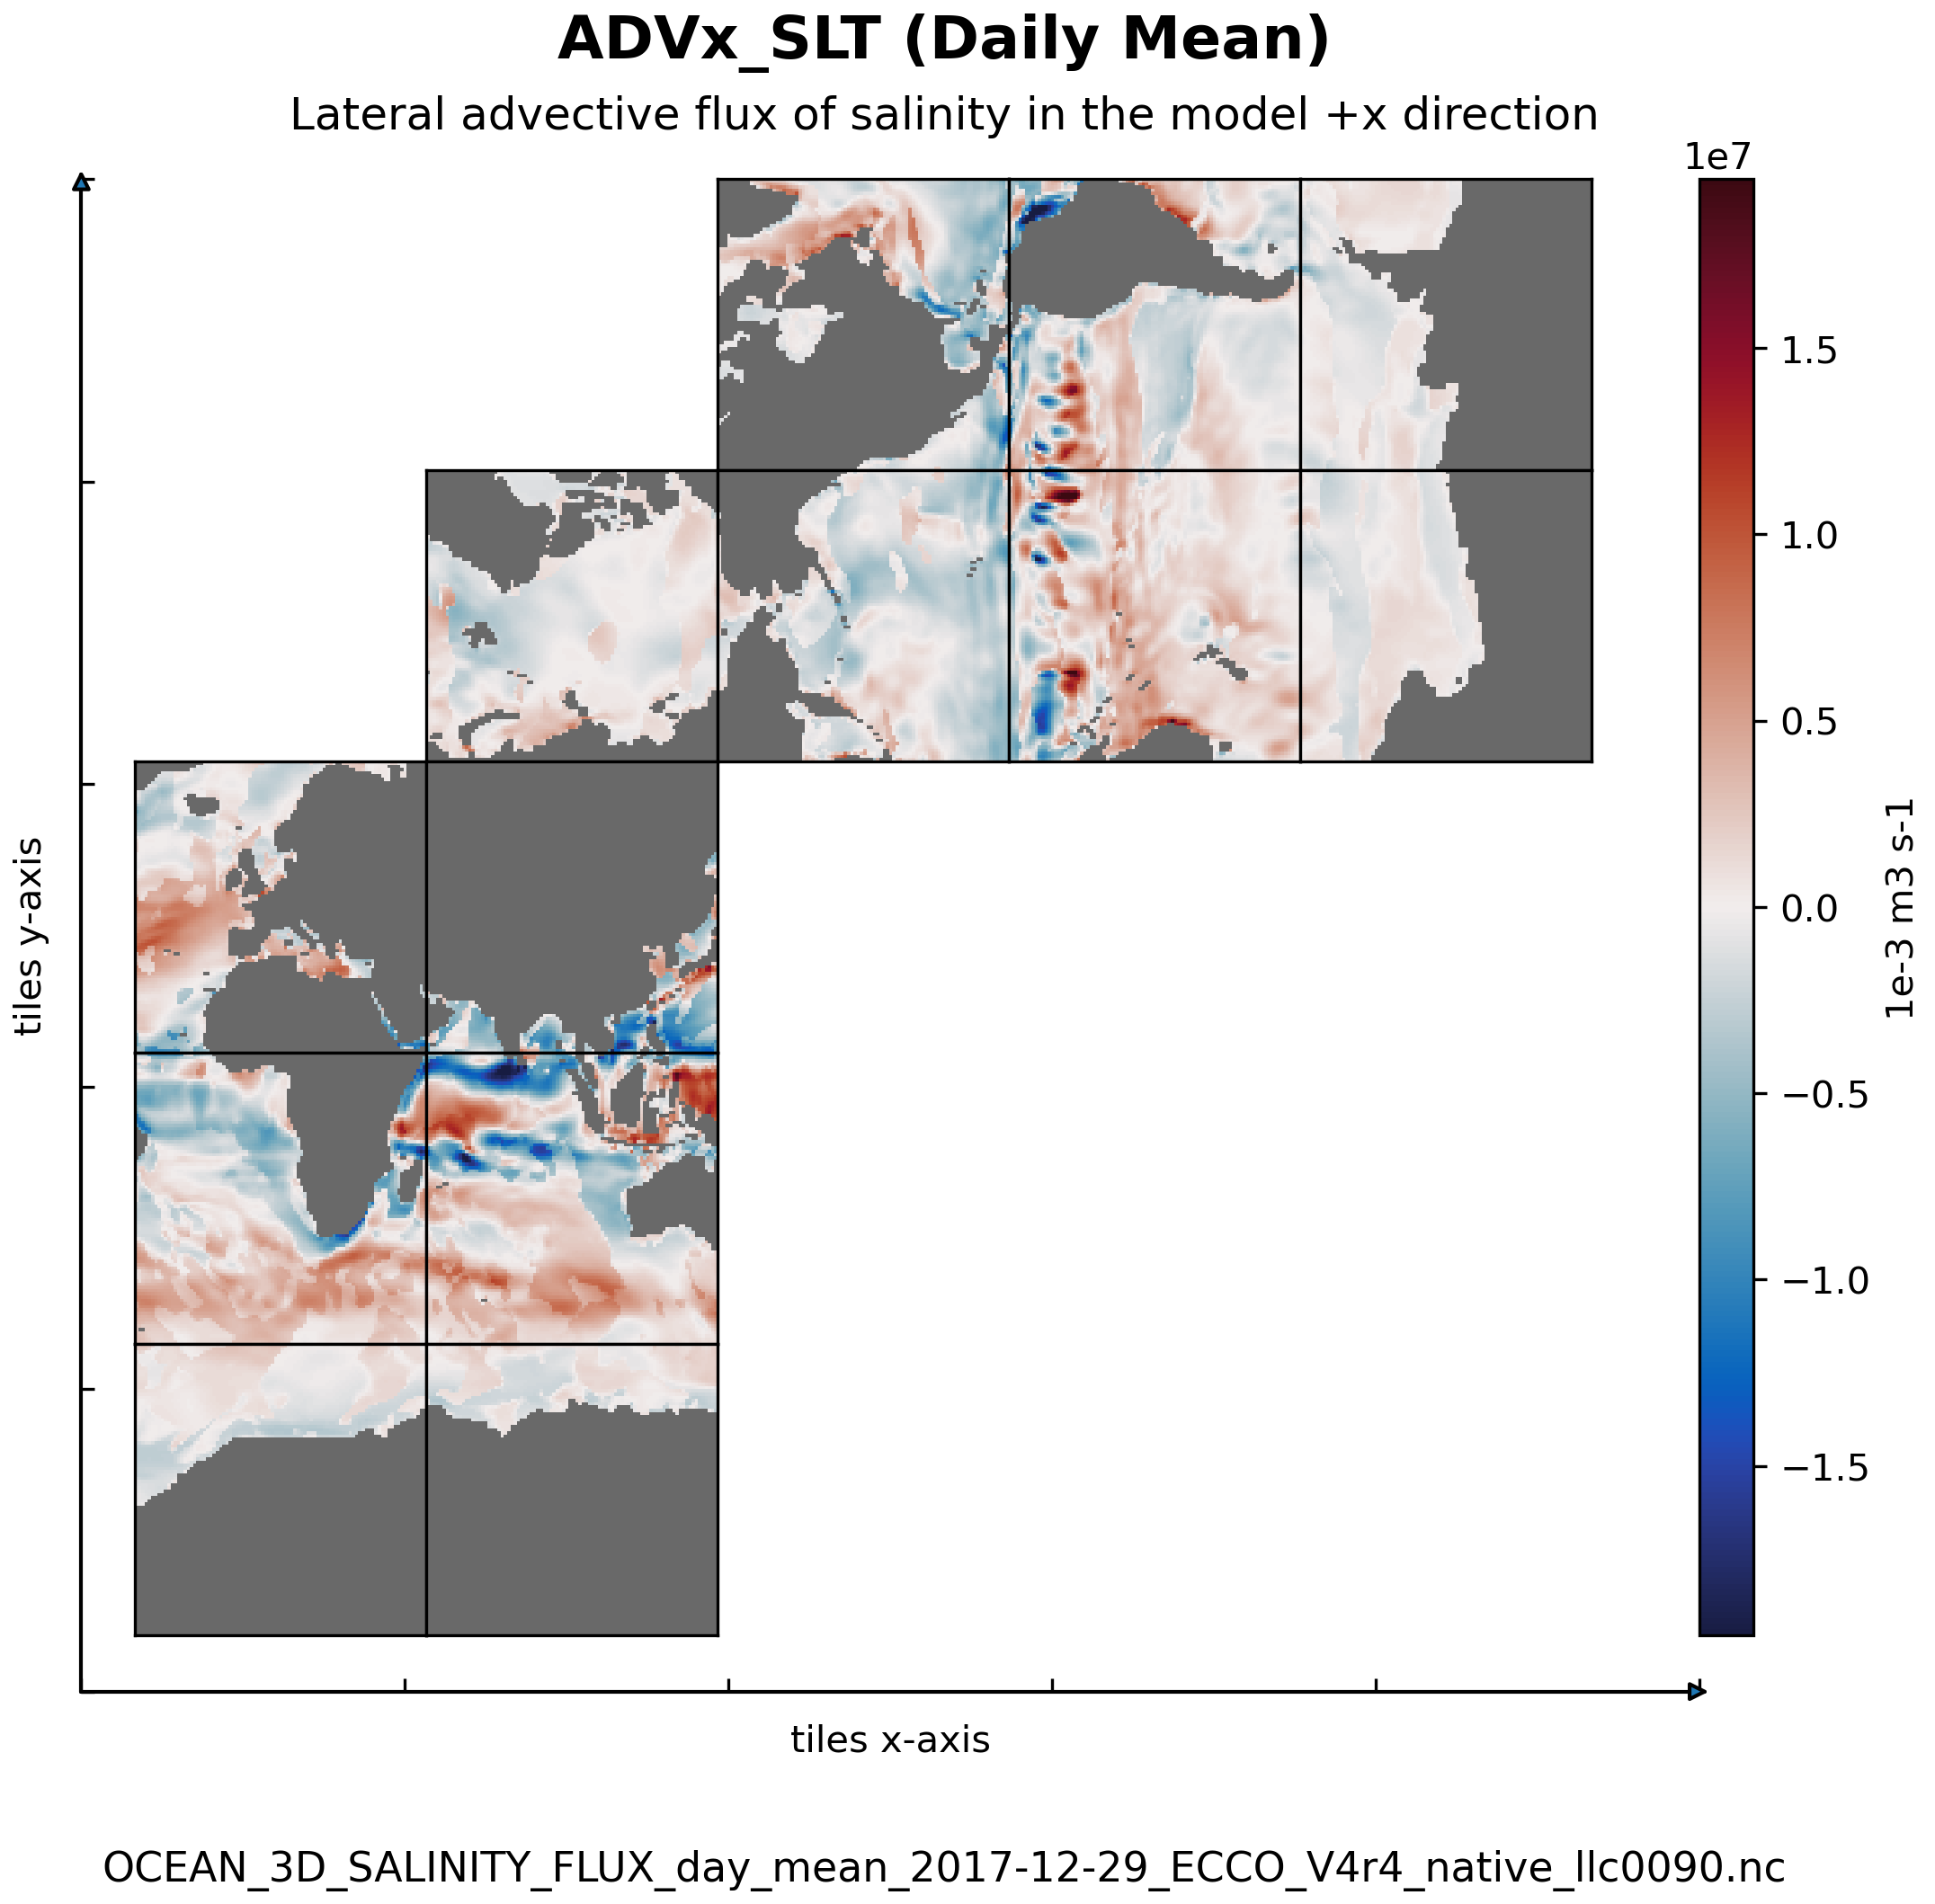
\includegraphics[scale=0.5]{../images/plots/native_plots/Ocean_Three-Dimensional_Salinity_Fluxes/ADVx_SLT.png}
\caption{\\Dataset: OCEAN\_3D\_SALINITY\_FLUX\\Variable: ADVx\_SLT}
\label{tab:table-OCEAN_3D_SALINITY_FLUX_ADVx_SLT-Plot}
\end{figure}
\pagebreak
\subsubsection{Native Variable ADVy\_SLT}
\begin{longtable}{|p{0.06\textwidth}|p{0.41\textwidth}|p{0.39\textwidth}|p{0.06\textwidth}|}
\caption{CDL description of OCEAN\_3D\_SALINITY\_FLUX's ADVy\_SLT variable}
\label{tab:table-OCEAN_3D_SALINITY_FLUX_ADVy_SLT} \\ 
\hline \endhead \hline \endfoot
\rowcolor{lightgray} \textbf{Storage Type} & \textbf{Variable Name} & \textbf{Description} & \textbf{Unit} \\ \hline
float32 & ADVy\_SLT & Lateral advective flux of salinity in the model +y direction & 1e-3 m3 s-1 \\ \hline
\rowcolor{lightgray}  \multicolumn{4}{|p{1.00\textwidth}|}{\textbf{CDL Description}} \\ \hline
\multicolumn{4}{|p{1.00\textwidth}|}{\makecell{\parbox{1\textwidth}{float32 ADVy\_SLT(time, k, tile, j\_g, i)\\
\hspace*{0.5cm}ADVy\_SLT: \_FillValue = 9.96921e+36\\
\hspace*{0.5cm}ADVy\_SLT: long\_name = Lateral advective flux of salinity in the model +y direction\\
\hspace*{0.5cm}ADVy\_SLT: units = 1e: 3 m3 s: 1\\
\hspace*{0.5cm}ADVy\_SLT: mate = ADVx\_SLT\\
\hspace*{0.5cm}ADVy\_SLT: coverage\_content\_type = modelResult\\
\hspace*{0.5cm}ADVy\_SLT: direction = >0 increases salinity (SALT)\\
\hspace*{0.5cm}ADVy\_SLT: coordinates = Z time\\
\hspace*{0.5cm}ADVy\_SLT: valid\_min = : 137905760.0\\
\hspace*{0.5cm}ADVy\_SLT: valid\_max = 164271664.0}}} \\ \hline
\rowcolor{lightgray} \multicolumn{4}{|p{1.00\textwidth}|}{\textbf{Comments}} \\ \hline
\multicolumn{4}{|p{1\textwidth}|}{Lateral advective flux of salinity (SALT) in the +y direction through the 'v' face of the tracer cell on the native model grid. Note: in the Arakawa-C grid, horizontal flux quantities are staggered relative to the tracer cells with indexing such that +ADVy\_SLT(i,j\_g,k) corresponds to +y fluxes through the 'v' face of the tracer cell at (i,j,k). Also, the model +y direction does not necessarily correspond to the geographical north-south direction because the x and y axes of the model's curvilinear lat-lon-cap (llc) grid have arbitrary orientations which vary within and across tiles. Salinity defined using CF convention 'Sea water salinity is the salt content of sea water, often on the Practical Salinity Scale of 1978. However, the unqualified term 'salinity' is generic and does not necessarily imply any particular method of calculation. The units of salinity are dimensionless and the units attribute should normally be given as 1e-3 or 0.001 i.e. parts per thousand.' see https://cfconventions.org/Data/cf-standard-names/73/build/cf-standard-name-table.html} \\ \hline
\end{longtable}

\begin{figure}[H]
\centering
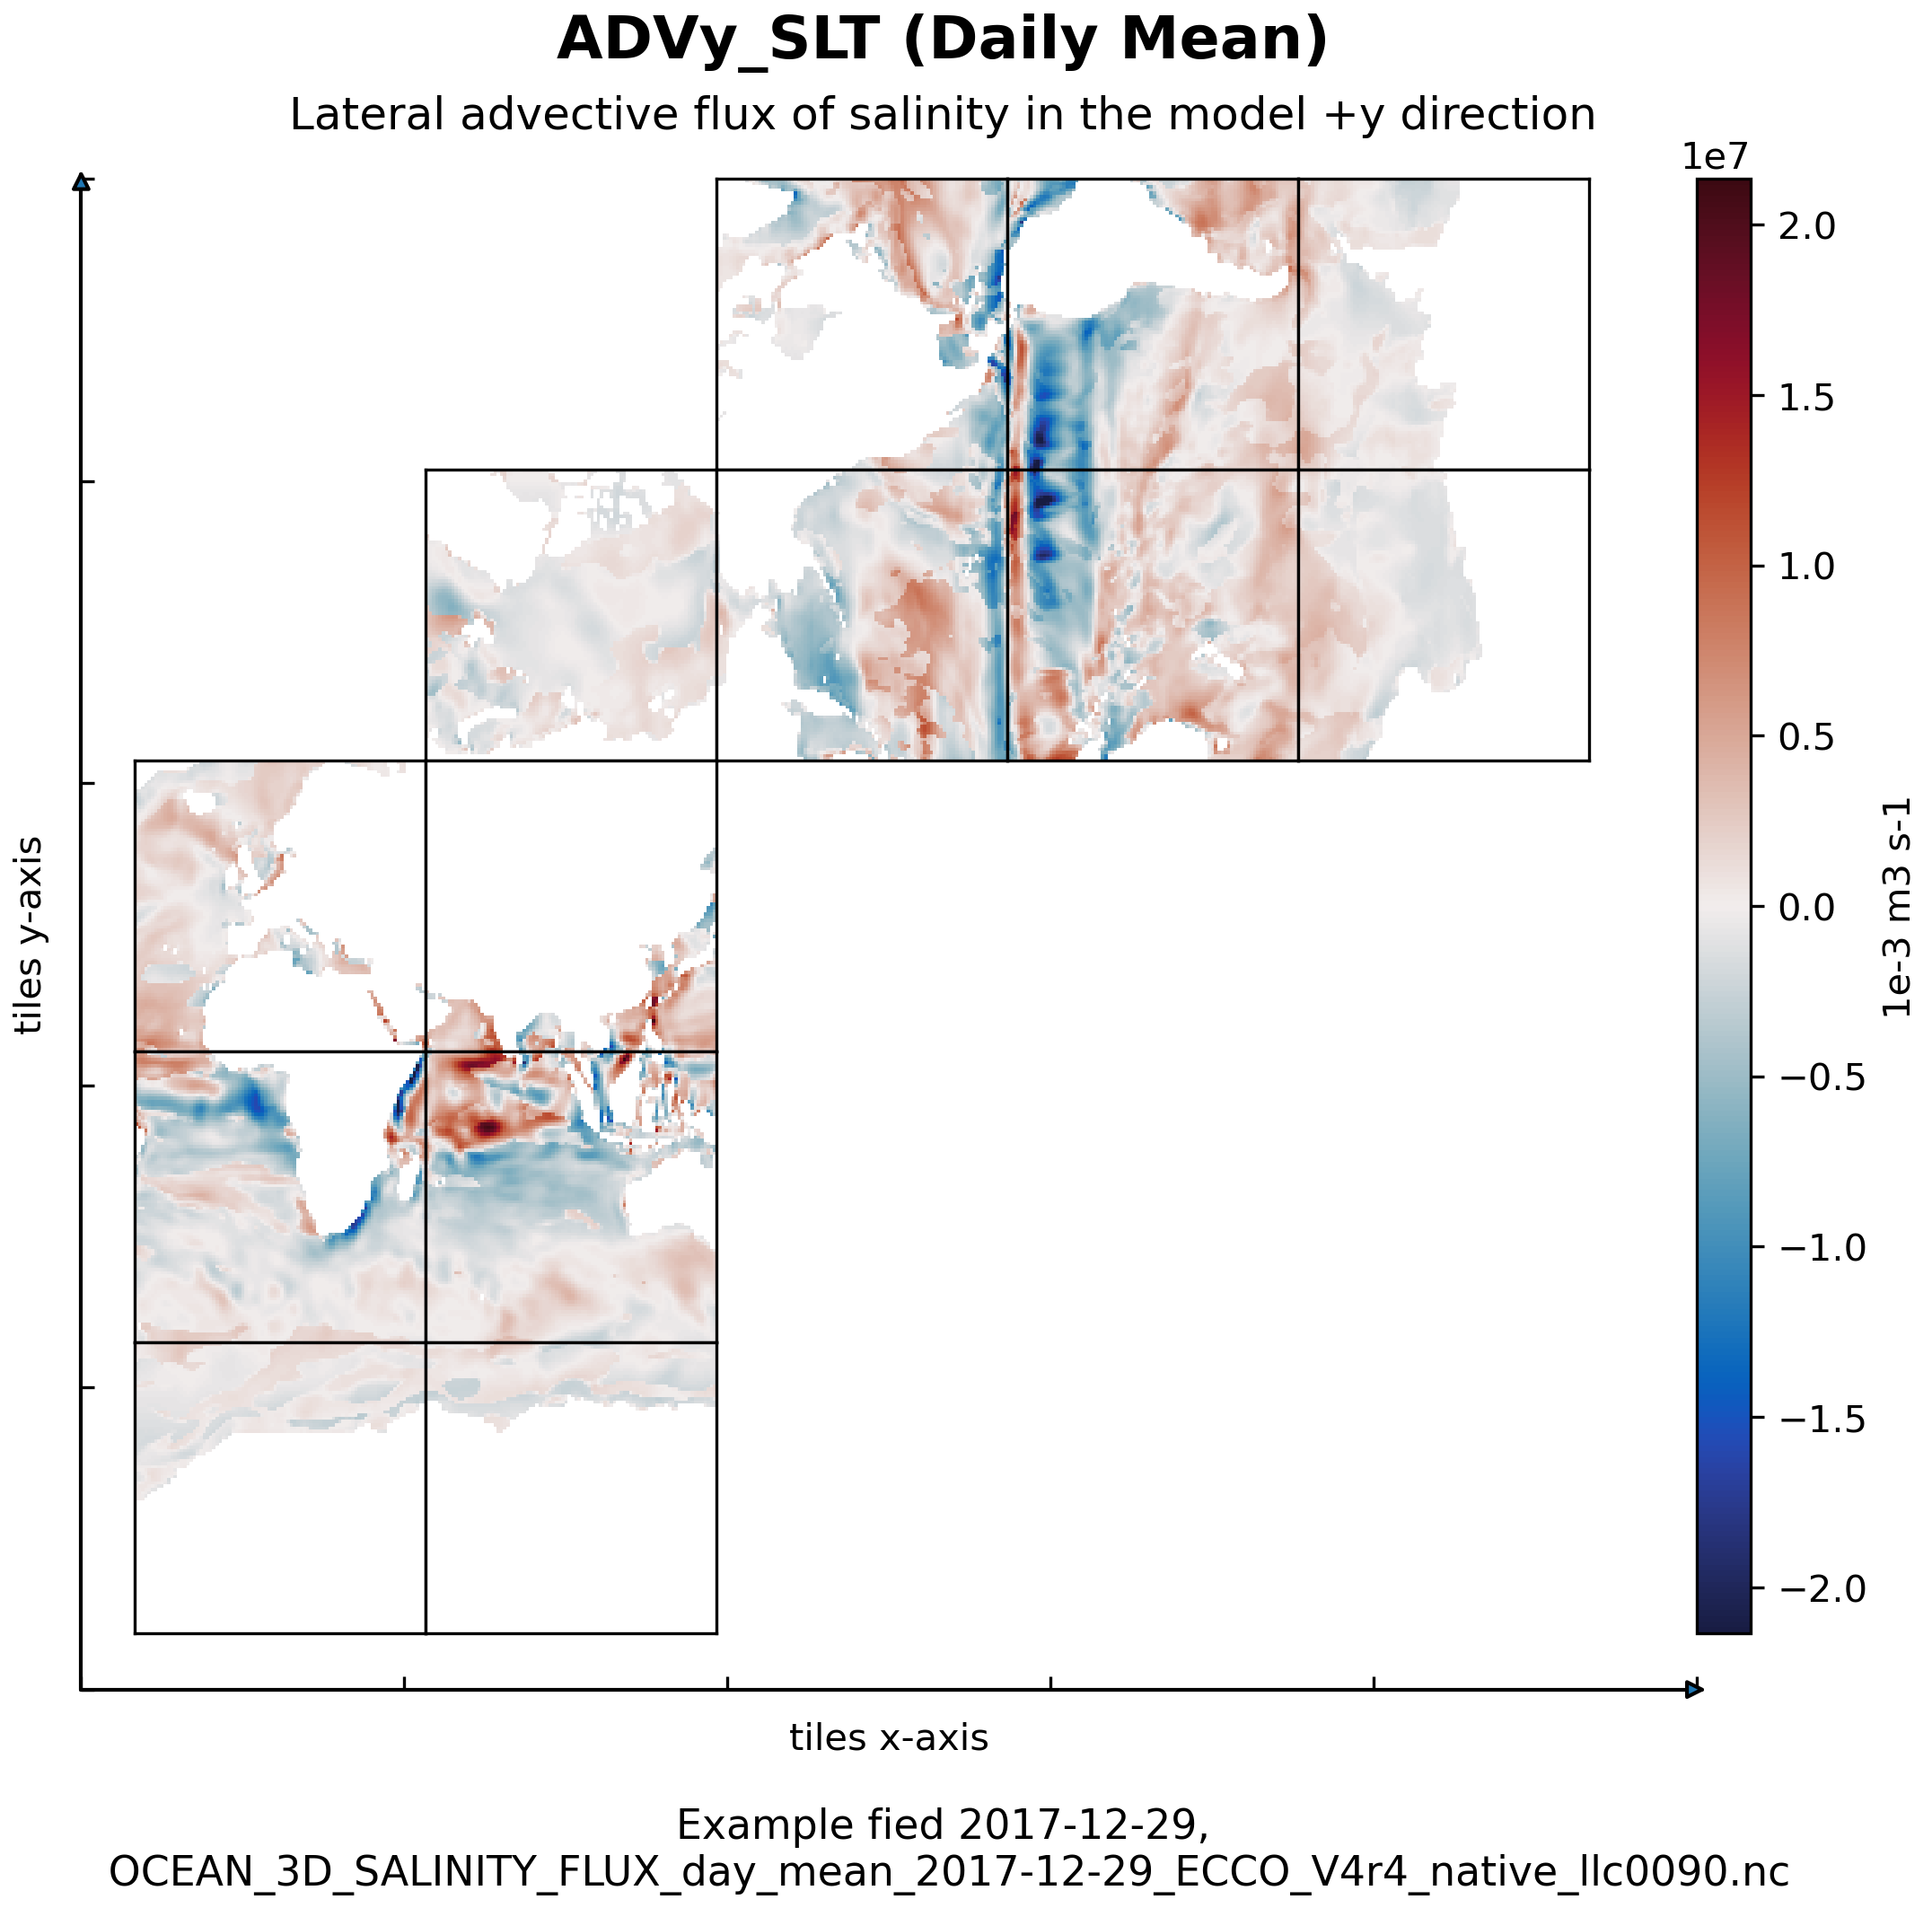
\includegraphics[scale=0.5]{../images/plots/native_plots/Ocean_Three-Dimensional_Salinity_Fluxes/ADVy_SLT.png}
\caption{\\Dataset: OCEAN\_3D\_SALINITY\_FLUX\\Variable: ADVy\_SLT}
\label{tab:table-OCEAN_3D_SALINITY_FLUX_ADVy_SLT-Plot}
\end{figure}
\pagebreak
\subsubsection{Native Variable DFrE\_SLT}
\begin{longtable}{|p{0.06\textwidth}|p{0.41\textwidth}|p{0.39\textwidth}|p{0.06\textwidth}|}
\caption{CDL description of OCEAN\_3D\_SALINITY\_FLUX's DFrE\_SLT variable}
\label{tab:table-OCEAN_3D_SALINITY_FLUX_DFrE_SLT} \\ 
\hline \endhead \hline \endfoot
\rowcolor{lightgray} \textbf{Storage Type} & \textbf{Variable Name} & \textbf{Description} & \textbf{Unit} \\ \hline
float32 & DFrE\_SLT & Vertical diffusive flux of salinity (explicit term) & 1e-3 m3 s-1 \\ \hline
\rowcolor{lightgray}  \multicolumn{4}{|p{1.00\textwidth}|}{\textbf{CDL Description}} \\ \hline
\multicolumn{4}{|p{1.00\textwidth}|}{\makecell{\parbox{1\textwidth}{float32 DFrE\_SLT(time, k\_l, tile, j, i)\\
\hspace*{0.5cm}DFrE\_SLT: \_FillValue = 9.96921e+36\\
\hspace*{0.5cm}DFrE\_SLT: long\_name = Vertical diffusive flux of salinity (explicit term)\\
\hspace*{0.5cm}DFrE\_SLT: units = 1e: 3 m3 s: 1\\
\hspace*{0.5cm}DFrE\_SLT: coverage\_content\_type = modelResult\\
\hspace*{0.5cm}DFrE\_SLT: direction = >0 decreases salinity (SALT)\\
\hspace*{0.5cm}DFrE\_SLT: coordinates = XC Zl YC time\\
\hspace*{0.5cm}DFrE\_SLT: valid\_min = : 1074719.375\\
\hspace*{0.5cm}DFrE\_SLT: valid\_max = 471215.75}}} \\ \hline
\rowcolor{lightgray} \multicolumn{4}{|p{1.00\textwidth}|}{\textbf{Comments}} \\ \hline
\multicolumn{4}{|p{1\textwidth}|}{The explicit term of the vertical diffusive flux of salinity (SALT) in the +z direction through the top 'w' face of the tracer cell on the native model grid. In the ECCO V4r4 model, an implicit scheme is used to calculate vertical diffusive tracer fluxes due to background diffusivity and the Kwz component of the GM-Redi tensor (vertical flux as a function of vertical gradient) while an explicit scheme is used to calculate the vertical diffusive fluxes from the Kwx and Kwy components of the GM-Redi tensor (vertical flux as a function of horizontal gradient). Both implicit and explicit components of vertical diffusive flux of salinity are provided. Note: in the Arakawa-C grid, vertical flux quantities are staggered relative to the tracer cells with indexing such that +DFrE\_SLT(i,j,k\_l) corresponds to upward +z fluxes through the top 'w' face of the tracer cell at (i,j,k). Salinity defined using CF convention 'Sea water salinity is the salt content of sea water, often on the Practical Salinity Scale of 1978. However, the unqualified term 'salinity' is generic and does not necessarily imply any particular method of calculation. The units of salinity are dimensionless and the units attribute should normally be given as 1e-3 or 0.001 i.e. parts per thousand.' see https://cfconventions.org/Data/cf-standard-names/73/build/cf-standard-name-table.html} \\ \hline
\end{longtable}

\begin{figure}[H]
\centering
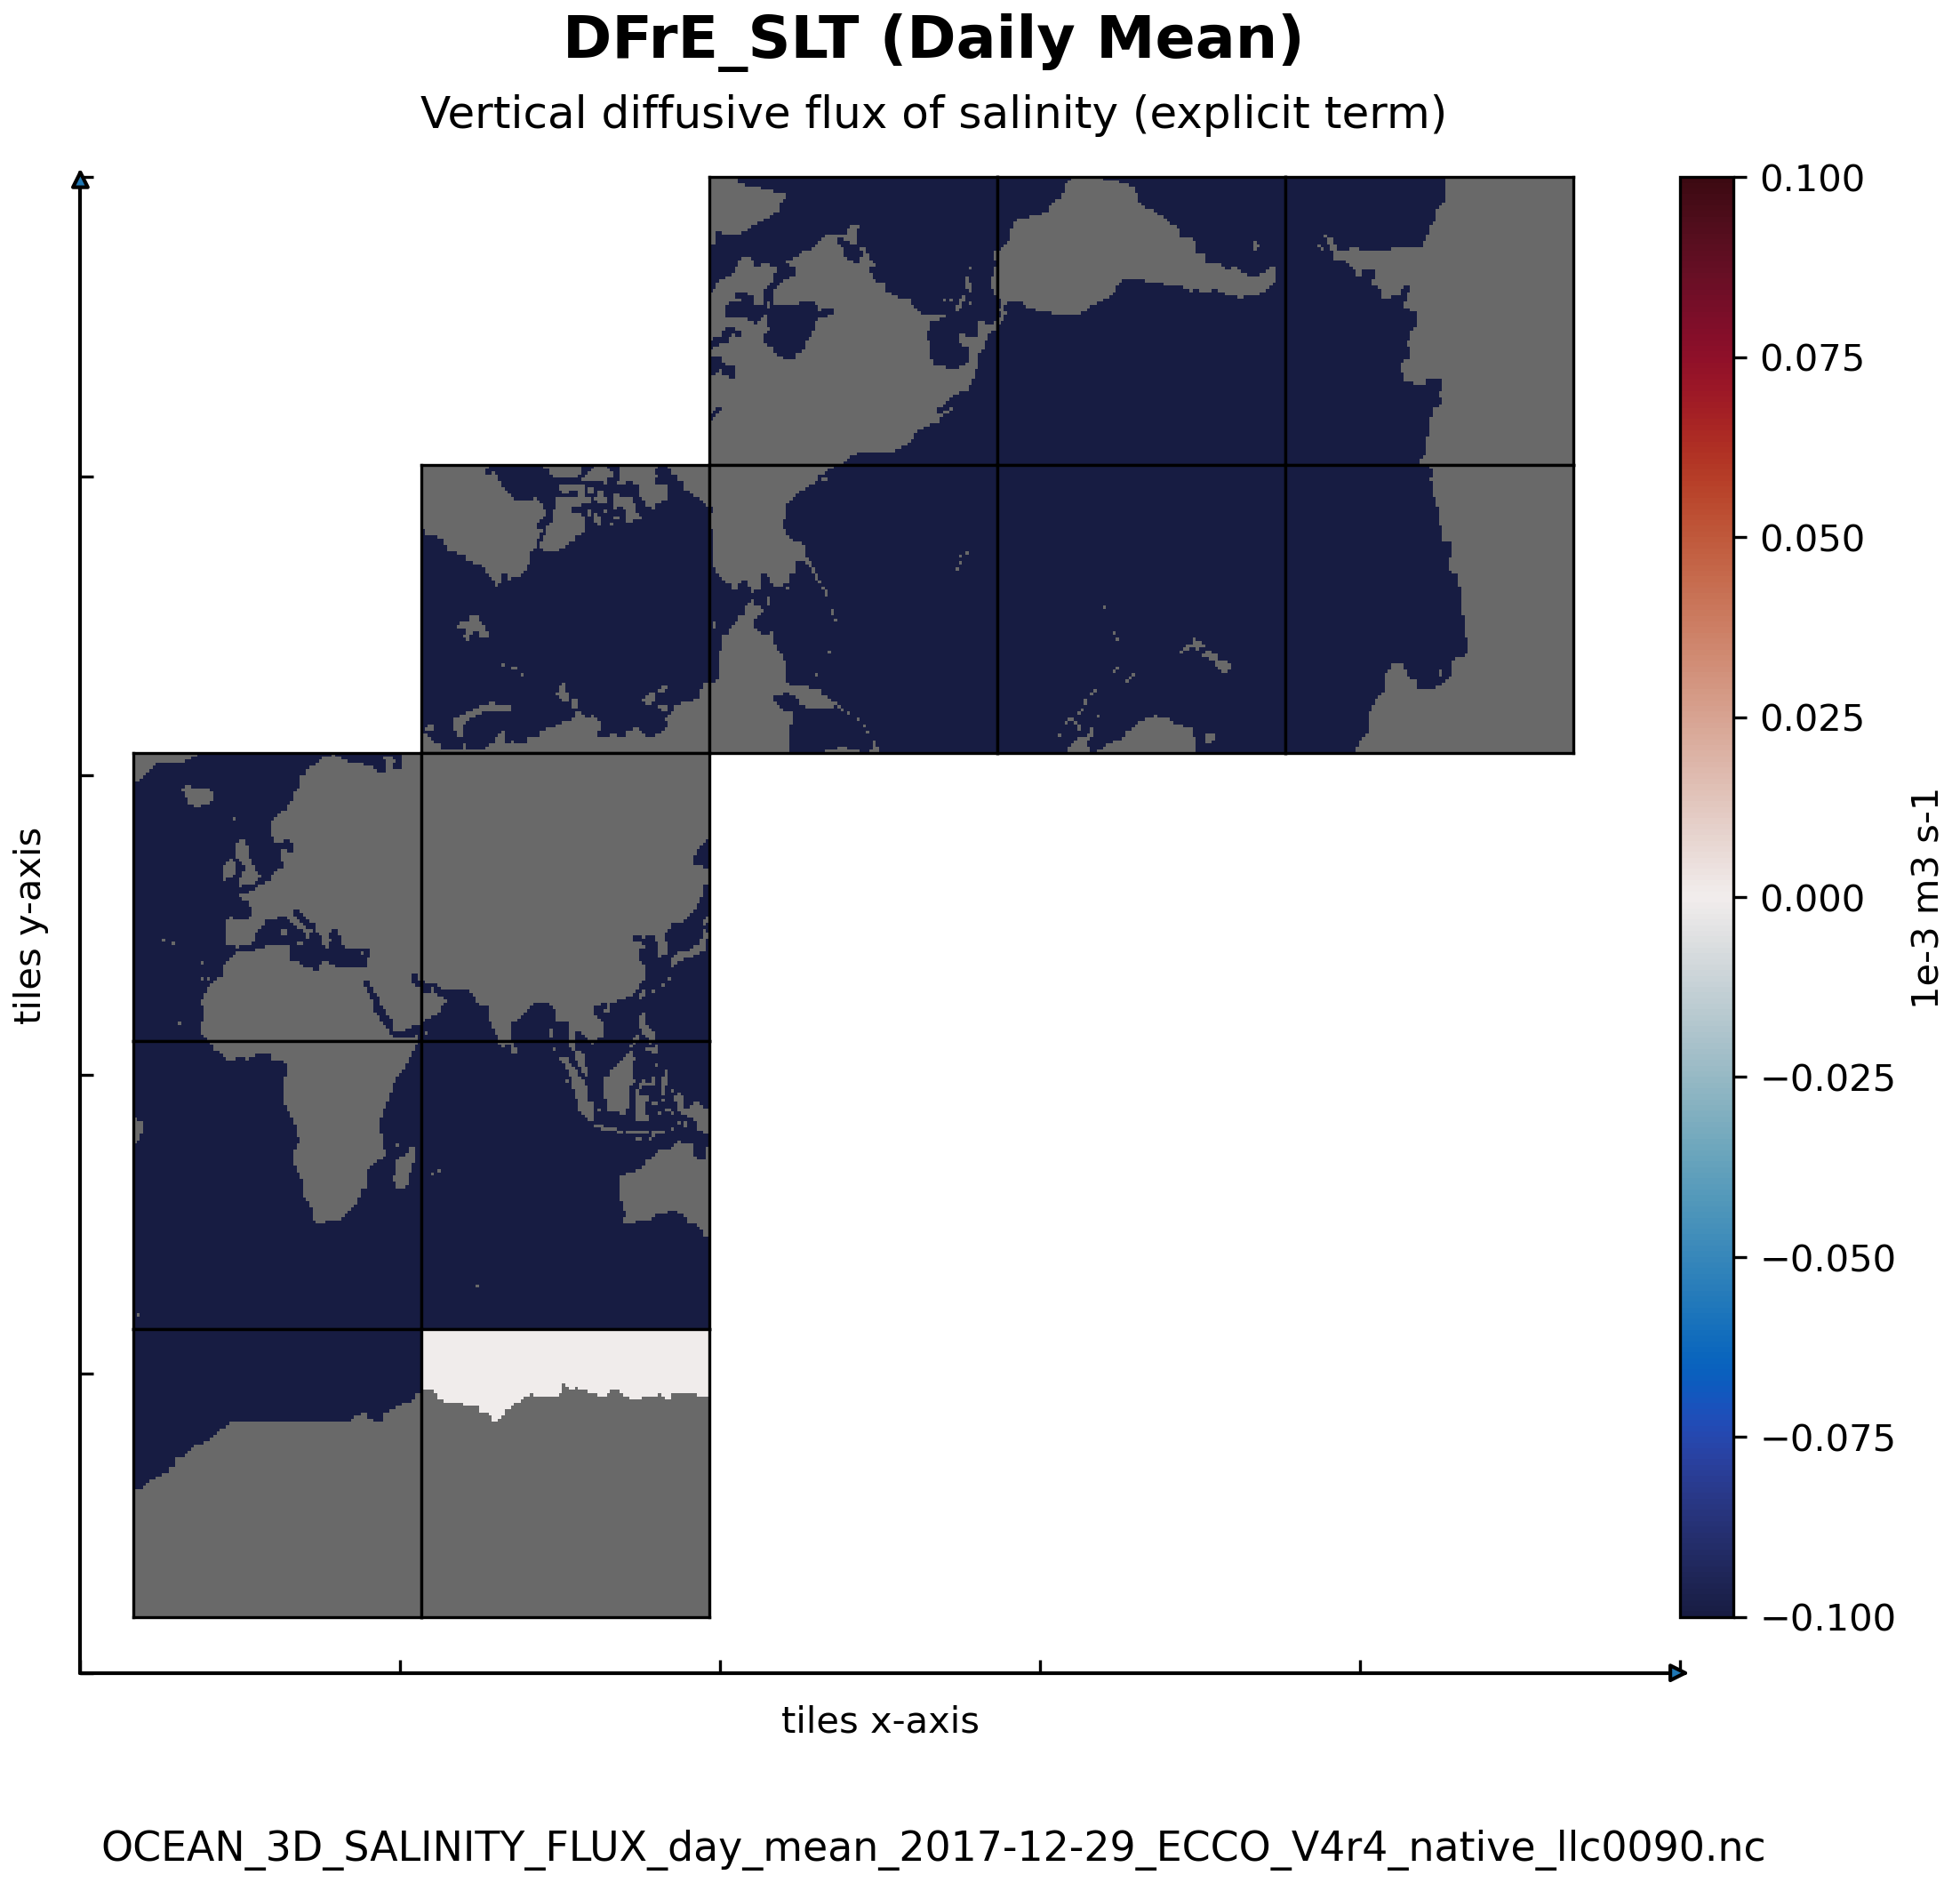
\includegraphics[scale=0.5]{../images/plots/native_plots/Ocean_Three-Dimensional_Salinity_Fluxes/DFrE_SLT.png}
\caption{\\Dataset: OCEAN\_3D\_SALINITY\_FLUX\\Variable: DFrE\_SLT}
\label{tab:table-OCEAN_3D_SALINITY_FLUX_DFrE_SLT-Plot}
\end{figure}
\pagebreak
\subsubsection{Native Variable DFrI\_SLT}
\begin{longtable}{|p{0.06\textwidth}|p{0.41\textwidth}|p{0.39\textwidth}|p{0.06\textwidth}|}
\caption{CDL description of OCEAN\_3D\_SALINITY\_FLUX's DFrI\_SLT variable}
\label{tab:table-OCEAN_3D_SALINITY_FLUX_DFrI_SLT} \\ 
\hline \endhead \hline \endfoot
\rowcolor{lightgray} \textbf{Storage Type} & \textbf{Variable Name} & \textbf{Description} & \textbf{Unit} \\ \hline
float32 & DFrI\_SLT & Vertical diffusive flux of salinity (implicit term) & 1e-3 m3 s-1 \\ \hline
\rowcolor{lightgray}  \multicolumn{4}{|p{1.00\textwidth}|}{\textbf{CDL Description}} \\ \hline
\multicolumn{4}{|p{1.00\textwidth}|}{\makecell{\parbox{1\textwidth}{float32 DFrI\_SLT(time, k\_l, tile, j, i)\\
\hspace*{0.5cm}DFrI\_SLT: \_FillValue = 9.96921e+36\\
\hspace*{0.5cm}DFrI\_SLT: long\_name = Vertical diffusive flux of salinity (implicit term)\\
\hspace*{0.5cm}DFrI\_SLT: units = 1e: 3 m3 s: 1\\
\hspace*{0.5cm}DFrI\_SLT: coverage\_content\_type = modelResult\\
\hspace*{0.5cm}DFrI\_SLT: direction = >0 decreases salinity (SALT)\\
\hspace*{0.5cm}DFrI\_SLT: coordinates = XC Zl YC time\\
\hspace*{0.5cm}DFrI\_SLT: valid\_min = : 30609048.0\\
\hspace*{0.5cm}DFrI\_SLT: valid\_max = 3197643.0}}} \\ \hline
\rowcolor{lightgray} \multicolumn{4}{|p{1.00\textwidth}|}{\textbf{Comments}} \\ \hline
\multicolumn{4}{|p{1\textwidth}|}{The implicit term of the vertical diffusive flux of salinity (SALT) in the +z direction through the top 'w' face of the tracer cell on the native model grid. In the ECCO V4r4 model, an implicit scheme is used to calculate vertical diffusive tracer fluxes due to background diffusivity and the Kwz component of the GM-Redi tensor (vertical flux as a function of vertical gradient) while an explicit scheme is used to calculate the vertical diffusive fluxes from the Kwx and Kwy components of the GM-Redi tensor (vertical flux as a function of horizontal gradient). Both implicit and explicit components of vertical diffusive flux of salinity are provided. Note: in the Arakawa-C grid, vertical flux quantities are staggered relative to the tracer cells with indexing such that +DFrI\_SLT(i,j,k\_l) corresponds to upward +z fluxes through the top face 'w' of the tracer cell at (i,j,k). Salinity defined using CF convention 'Sea water salinity is the salt content of sea water, often on the Practical Salinity Scale of 1978. However, the unqualified term 'salinity' is generic and does not necessarily imply any particular method of calculation. The units of salinity are dimensionless and the units attribute should normally be given as 1e-3 or 0.001 i.e. parts per thousand.' see https://cfconventions.org/Data/cf-standard-names/73/build/cf-standard-name-table.html} \\ \hline
\end{longtable}

\begin{figure}[H]
\centering
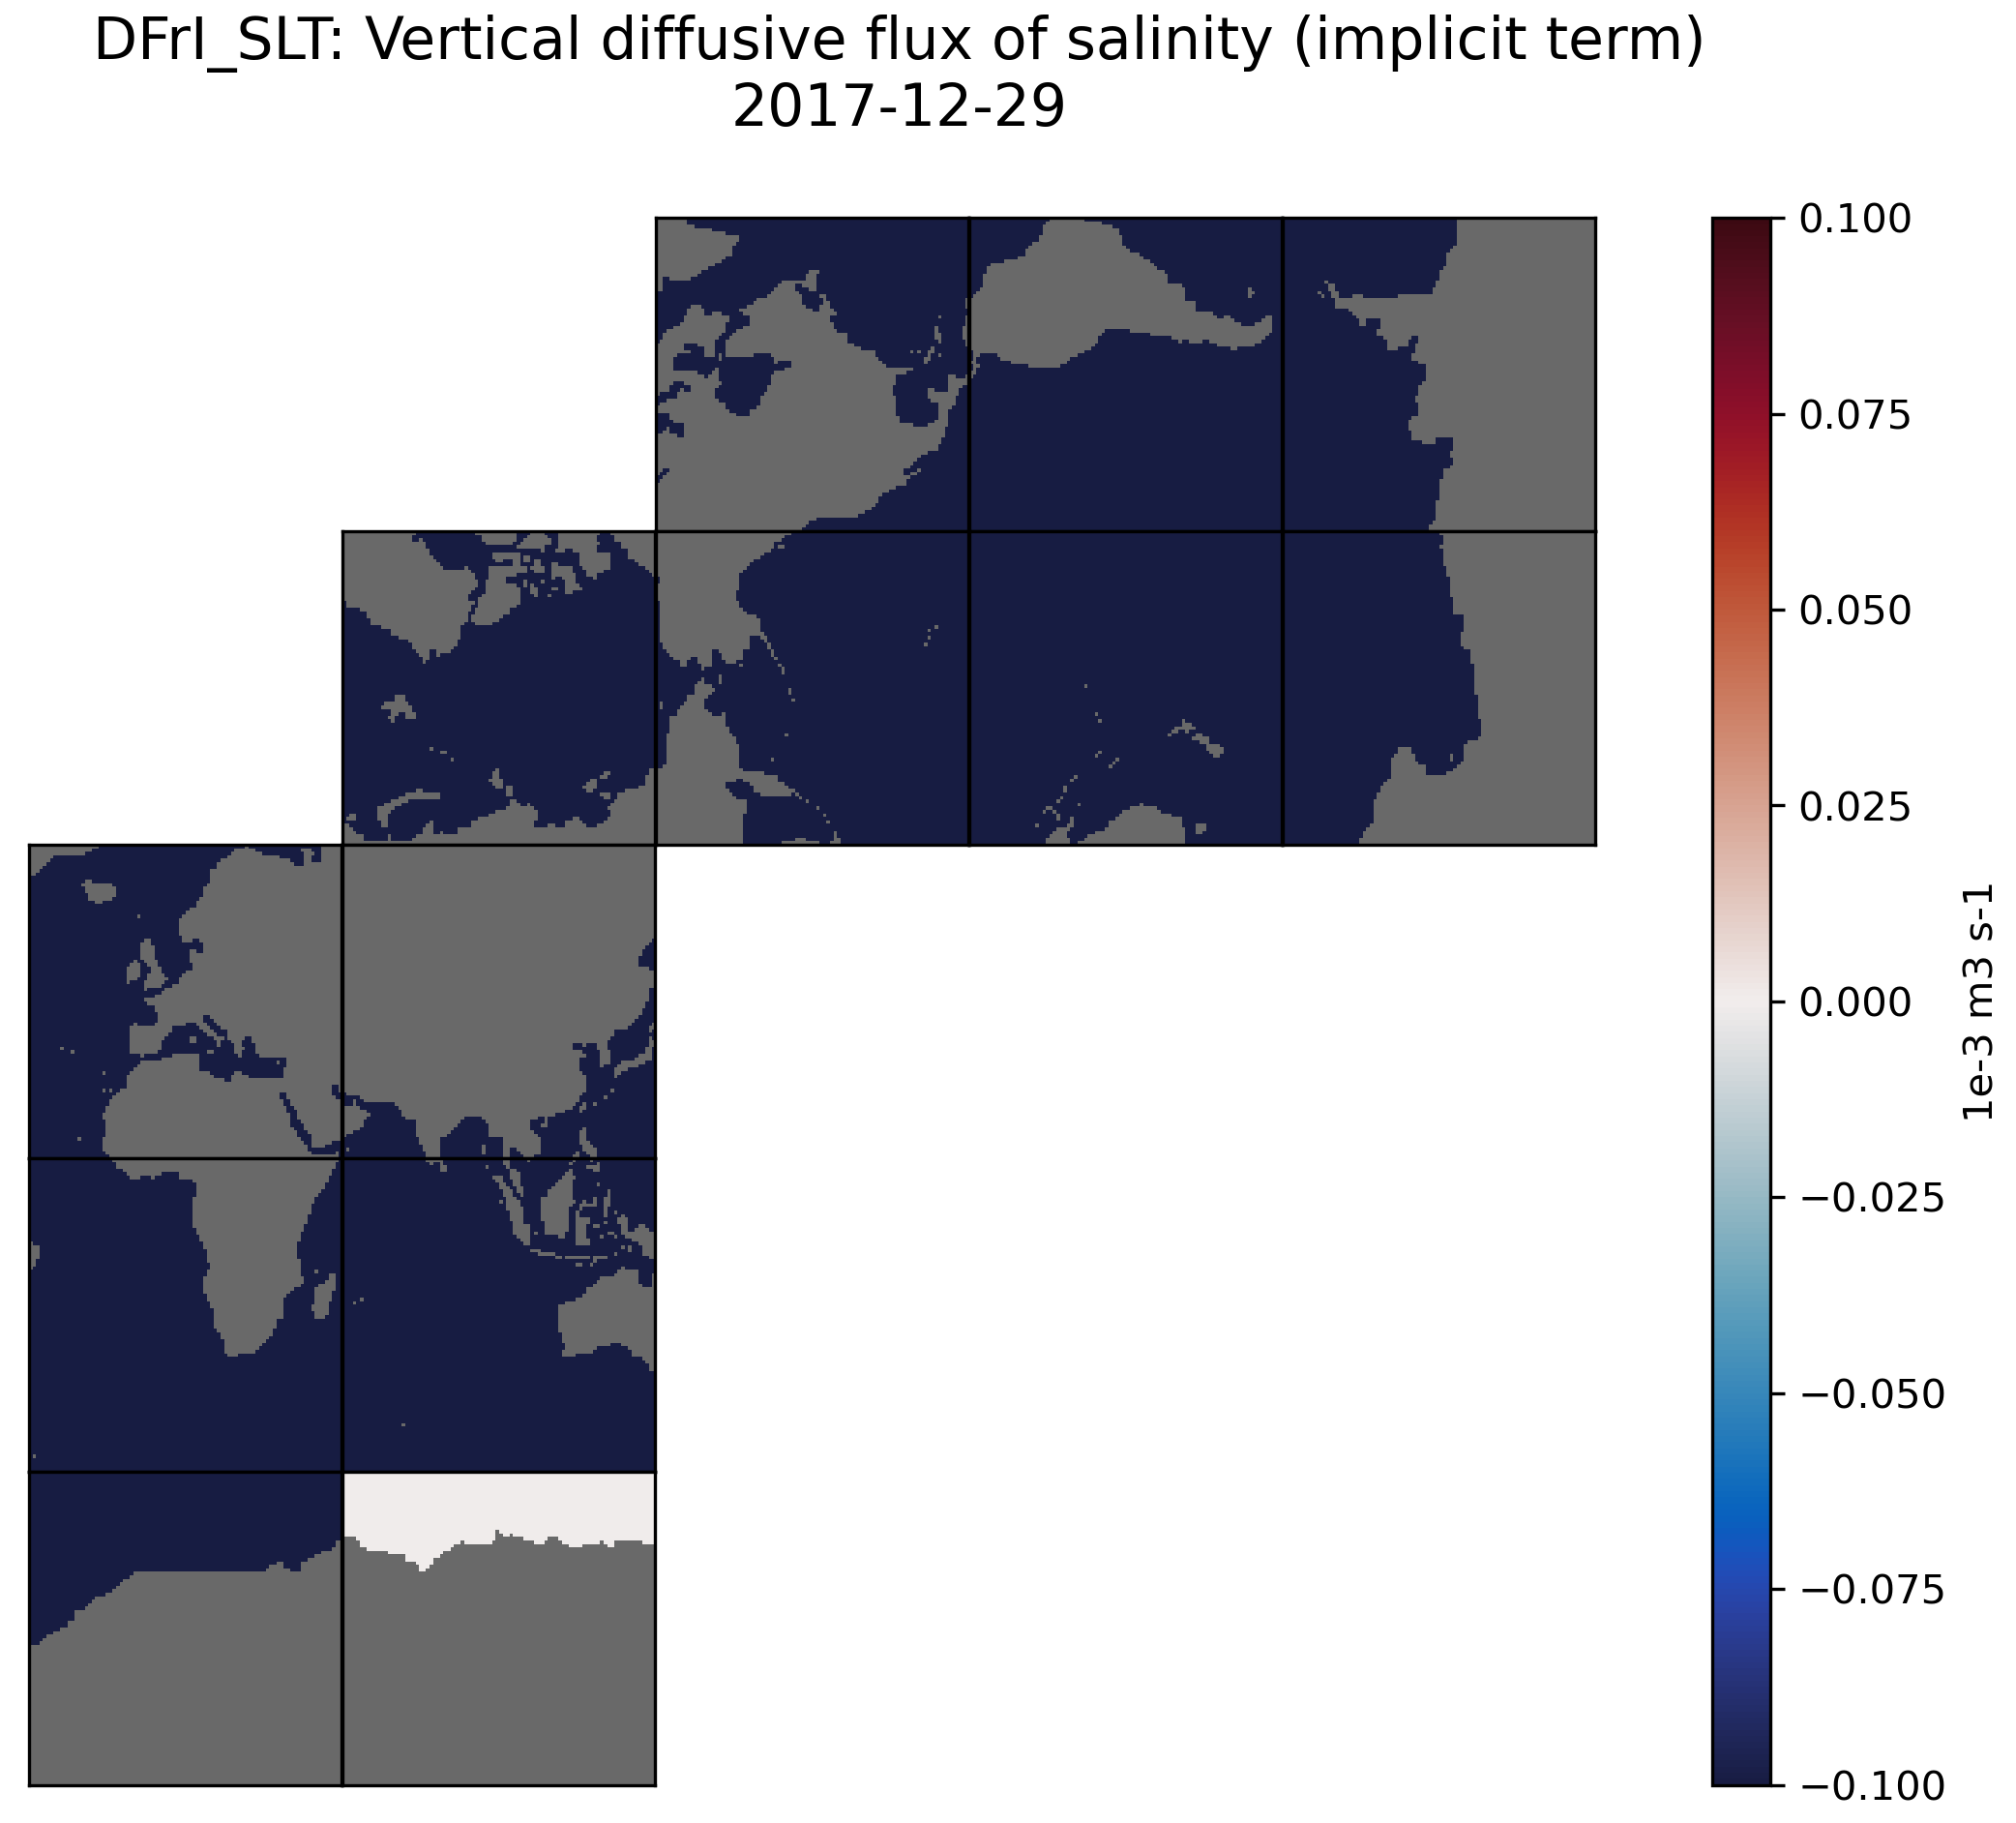
\includegraphics[scale=0.5]{../images/plots/native_plots/Ocean_Three-Dimensional_Salinity_Fluxes/DFrI_SLT.png}
\caption{\\Dataset: OCEAN\_3D\_SALINITY\_FLUX\\Variable: DFrI\_SLT}
\label{tab:table-OCEAN_3D_SALINITY_FLUX_DFrI_SLT-Plot}
\end{figure}
\pagebreak
\subsubsection{Native Variable DFxE\_SLT}
\begin{longtable}{|p{0.06\textwidth}|p{0.41\textwidth}|p{0.39\textwidth}|p{0.06\textwidth}|}
\caption{CDL description of OCEAN\_3D\_SALINITY\_FLUX's DFxE\_SLT variable}
\label{tab:table-OCEAN_3D_SALINITY_FLUX_DFxE_SLT} \\ 
\hline \endhead \hline \endfoot
\rowcolor{lightgray} \textbf{Storage Type} & \textbf{Variable Name} & \textbf{Description} & \textbf{Unit} \\ \hline
float32 & DFxE\_SLT & Lateral diffusive flux of salinity in the model +x direction & 1e-3 m3 s-1 \\ \hline
\rowcolor{lightgray}  \multicolumn{4}{|p{1.00\textwidth}|}{\textbf{CDL Description}} \\ \hline
\multicolumn{4}{|p{1.00\textwidth}|}{\makecell{\parbox{1\textwidth}{float32 DFxE\_SLT(time, k, tile, j, i\_g)\\
\hspace*{0.5cm}DFxE\_SLT: \_FillValue = 9.96921e+36\\
\hspace*{0.5cm}DFxE\_SLT: long\_name = Lateral diffusive flux of salinity in the model +x direction\\
\hspace*{0.5cm}DFxE\_SLT: units = 1e: 3 m3 s: 1\\
\hspace*{0.5cm}DFxE\_SLT: mate = DFyE\_SLT\\
\hspace*{0.5cm}DFxE\_SLT: coverage\_content\_type = modelResult\\
\hspace*{0.5cm}DFxE\_SLT: direction = >0 increases salinity (SALT)\\
\hspace*{0.5cm}DFxE\_SLT: coordinates = Z time\\
\hspace*{0.5cm}DFxE\_SLT: valid\_min = : 125908.03125\\
\hspace*{0.5cm}DFxE\_SLT: valid\_max = 192716.484375}}} \\ \hline
\rowcolor{lightgray} \multicolumn{4}{|p{1.00\textwidth}|}{\textbf{Comments}} \\ \hline
\multicolumn{4}{|p{1\textwidth}|}{Lateral diffusive flux of salinity (SALT) in the +x direction through the 'u' face of the tracer cell on the native model grid. Note: in the Arakawa-C grid, horizontal flux quantities are staggered relative to the tracer cells with indexing such that +DFxE\_SLT(i\_g,j,k) corresponds to +x fluxes through the 'u' face of the tracer cell at (i,j,k). Also, the model +x direction does not necessarily correspond to the geographical east-west direction because the x and y axes of the model's curvilinear lat-lon-cap (llc) grid have arbitrary orientations which vary within and across tiles. Salinity defined using CF convention 'Sea water salinity is the salt content of sea water, often on the Practical Salinity Scale of 1978. However, the unqualified term 'salinity' is generic and does not necessarily imply any particular method of calculation. The units of salinity are dimensionless and the units attribute should normally be given as 1e-3 or 0.001 i.e. parts per thousand.' see https://cfconventions.org/Data/cf-standard-names/73/build/cf-standard-name-table.html} \\ \hline
\end{longtable}

\begin{figure}[H]
\centering
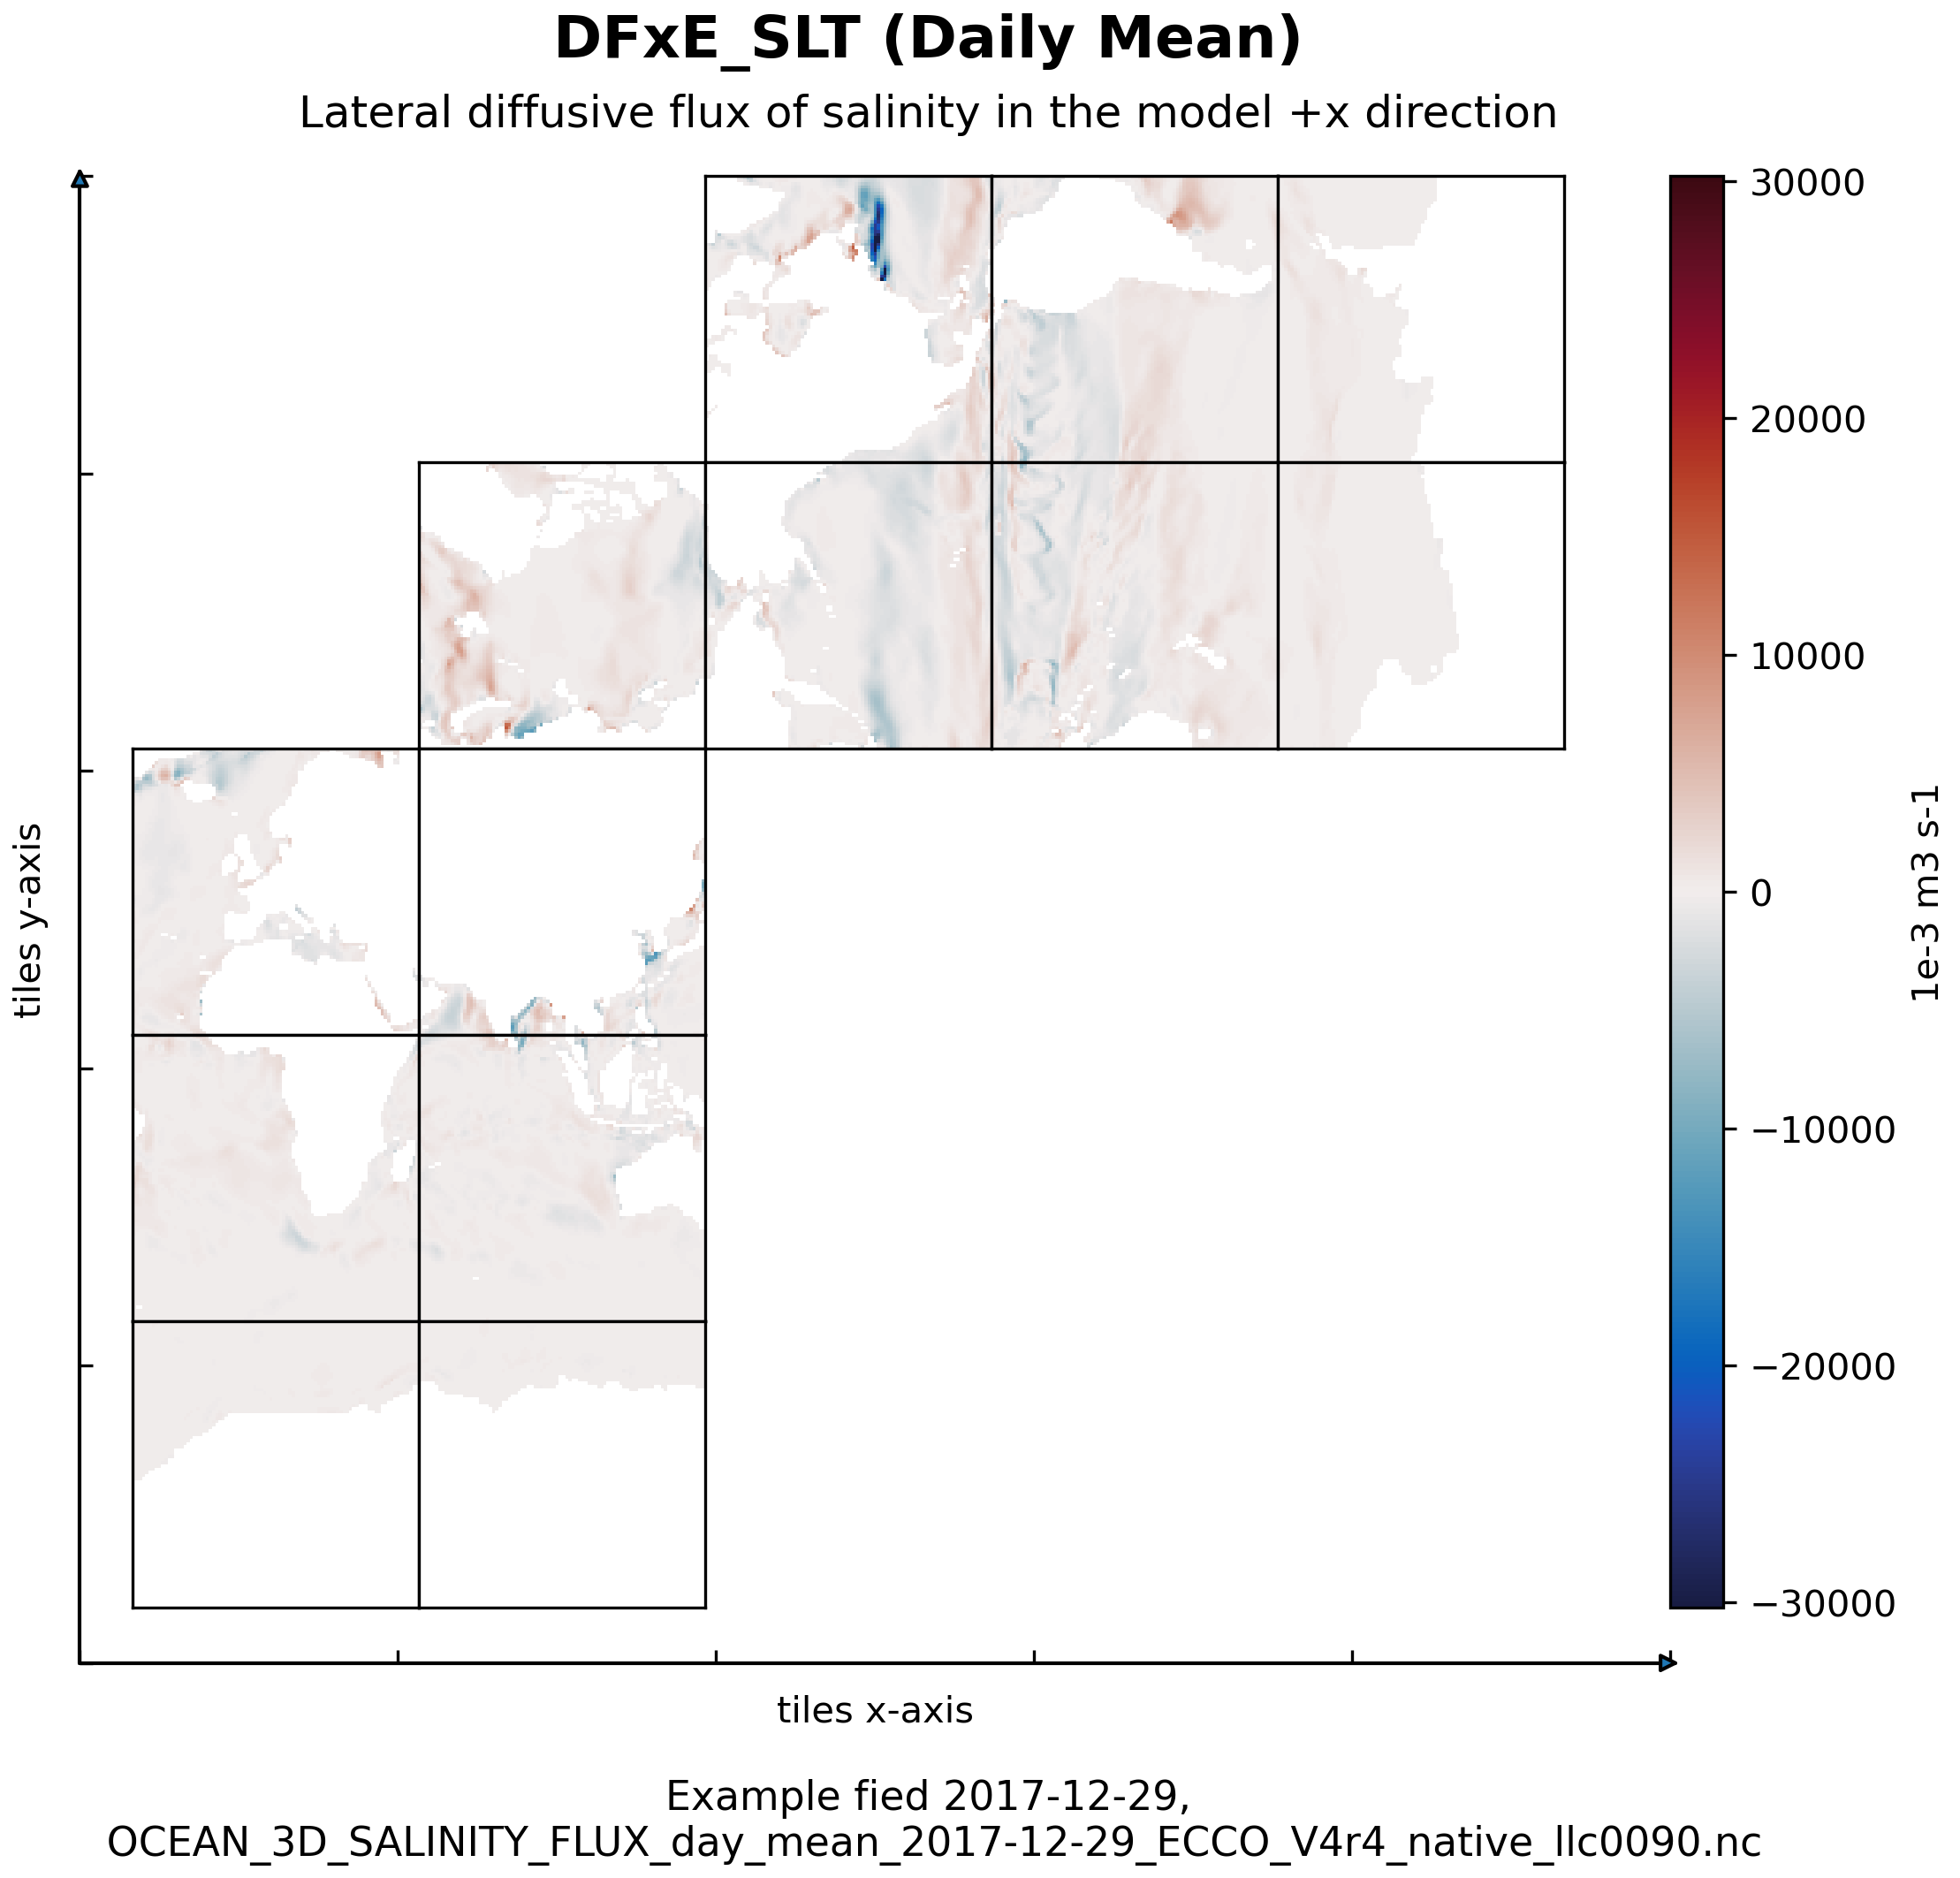
\includegraphics[scale=0.5]{../images/plots/native_plots/Ocean_Three-Dimensional_Salinity_Fluxes/DFxE_SLT.png}
\caption{\\Dataset: OCEAN\_3D\_SALINITY\_FLUX\\Variable: DFxE\_SLT}
\label{tab:table-OCEAN_3D_SALINITY_FLUX_DFxE_SLT-Plot}
\end{figure}
\pagebreak
\subsubsection{Native Variable DFyE\_SLT}
\begin{longtable}{|p{0.06\textwidth}|p{0.41\textwidth}|p{0.39\textwidth}|p{0.06\textwidth}|}
\caption{CDL description of OCEAN\_3D\_SALINITY\_FLUX's DFyE\_SLT variable}
\label{tab:table-OCEAN_3D_SALINITY_FLUX_DFyE_SLT} \\ 
\hline \endhead \hline \endfoot
\rowcolor{lightgray} \textbf{Storage Type} & \textbf{Variable Name} & \textbf{Description} & \textbf{Unit} \\ \hline
float32 & DFyE\_SLT & Lateral diffusive flux of salinity in the model +y direction & 1e-3 m3 s-1 \\ \hline
\rowcolor{lightgray}  \multicolumn{4}{|p{1.00\textwidth}|}{\textbf{CDL Description}} \\ \hline
\multicolumn{4}{|p{1.00\textwidth}|}{\makecell{\parbox{1\textwidth}{float32 DFyE\_SLT(time, k, tile, j\_g, i)\\
\hspace*{0.5cm}DFyE\_SLT: \_FillValue = 9.96921e+36\\
\hspace*{0.5cm}DFyE\_SLT: long\_name = Lateral diffusive flux of salinity in the model +y direction\\
\hspace*{0.5cm}DFyE\_SLT: units = 1e: 3 m3 s: 1\\
\hspace*{0.5cm}DFyE\_SLT: mate = DFxE\_SLT\\
\hspace*{0.5cm}DFyE\_SLT: coverage\_content\_type = modelResult\\
\hspace*{0.5cm}DFyE\_SLT: direction = >0 increases salinity (SALT)\\
\hspace*{0.5cm}DFyE\_SLT: coordinates = Z time\\
\hspace*{0.5cm}DFyE\_SLT: valid\_min = : 114959.2109375\\
\hspace*{0.5cm}DFyE\_SLT: valid\_max = 154227.140625}}} \\ \hline
\rowcolor{lightgray} \multicolumn{4}{|p{1.00\textwidth}|}{\textbf{Comments}} \\ \hline
\multicolumn{4}{|p{1\textwidth}|}{Lateral diffusive flux of salinity (SALT) in the +y direction through the 'v' face of the tracer cell on the native model grid. Note: in the Arakawa-C grid, horizontal flux quantities are staggered relative to the tracer cells with indexing such that +DFyE\_SLT(i,j\_g,k) corresponds to +y fluxes through the 'v' face of the tracer cell at (i,j,k). Also, the model +y direction does not necessarily correspond to the geographical north-south direction because the x and y axes of the model's curvilinear lat-lon-cap (llc) grid have arbitrary orientations which vary within and across tiles. Salinity defined using CF convention 'Sea water salinity is the salt content of sea water, often on the Practical Salinity Scale of 1978. However, the unqualified term 'salinity' is generic and does not necessarily imply any particular method of calculation. The units of salinity are dimensionless and the units attribute should normally be given as 1e-3 or 0.001 i.e. parts per thousand.' see https://cfconventions.org/Data/cf-standard-names/73/build/cf-standard-name-table.html} \\ \hline
\end{longtable}

\begin{figure}[H]
\centering
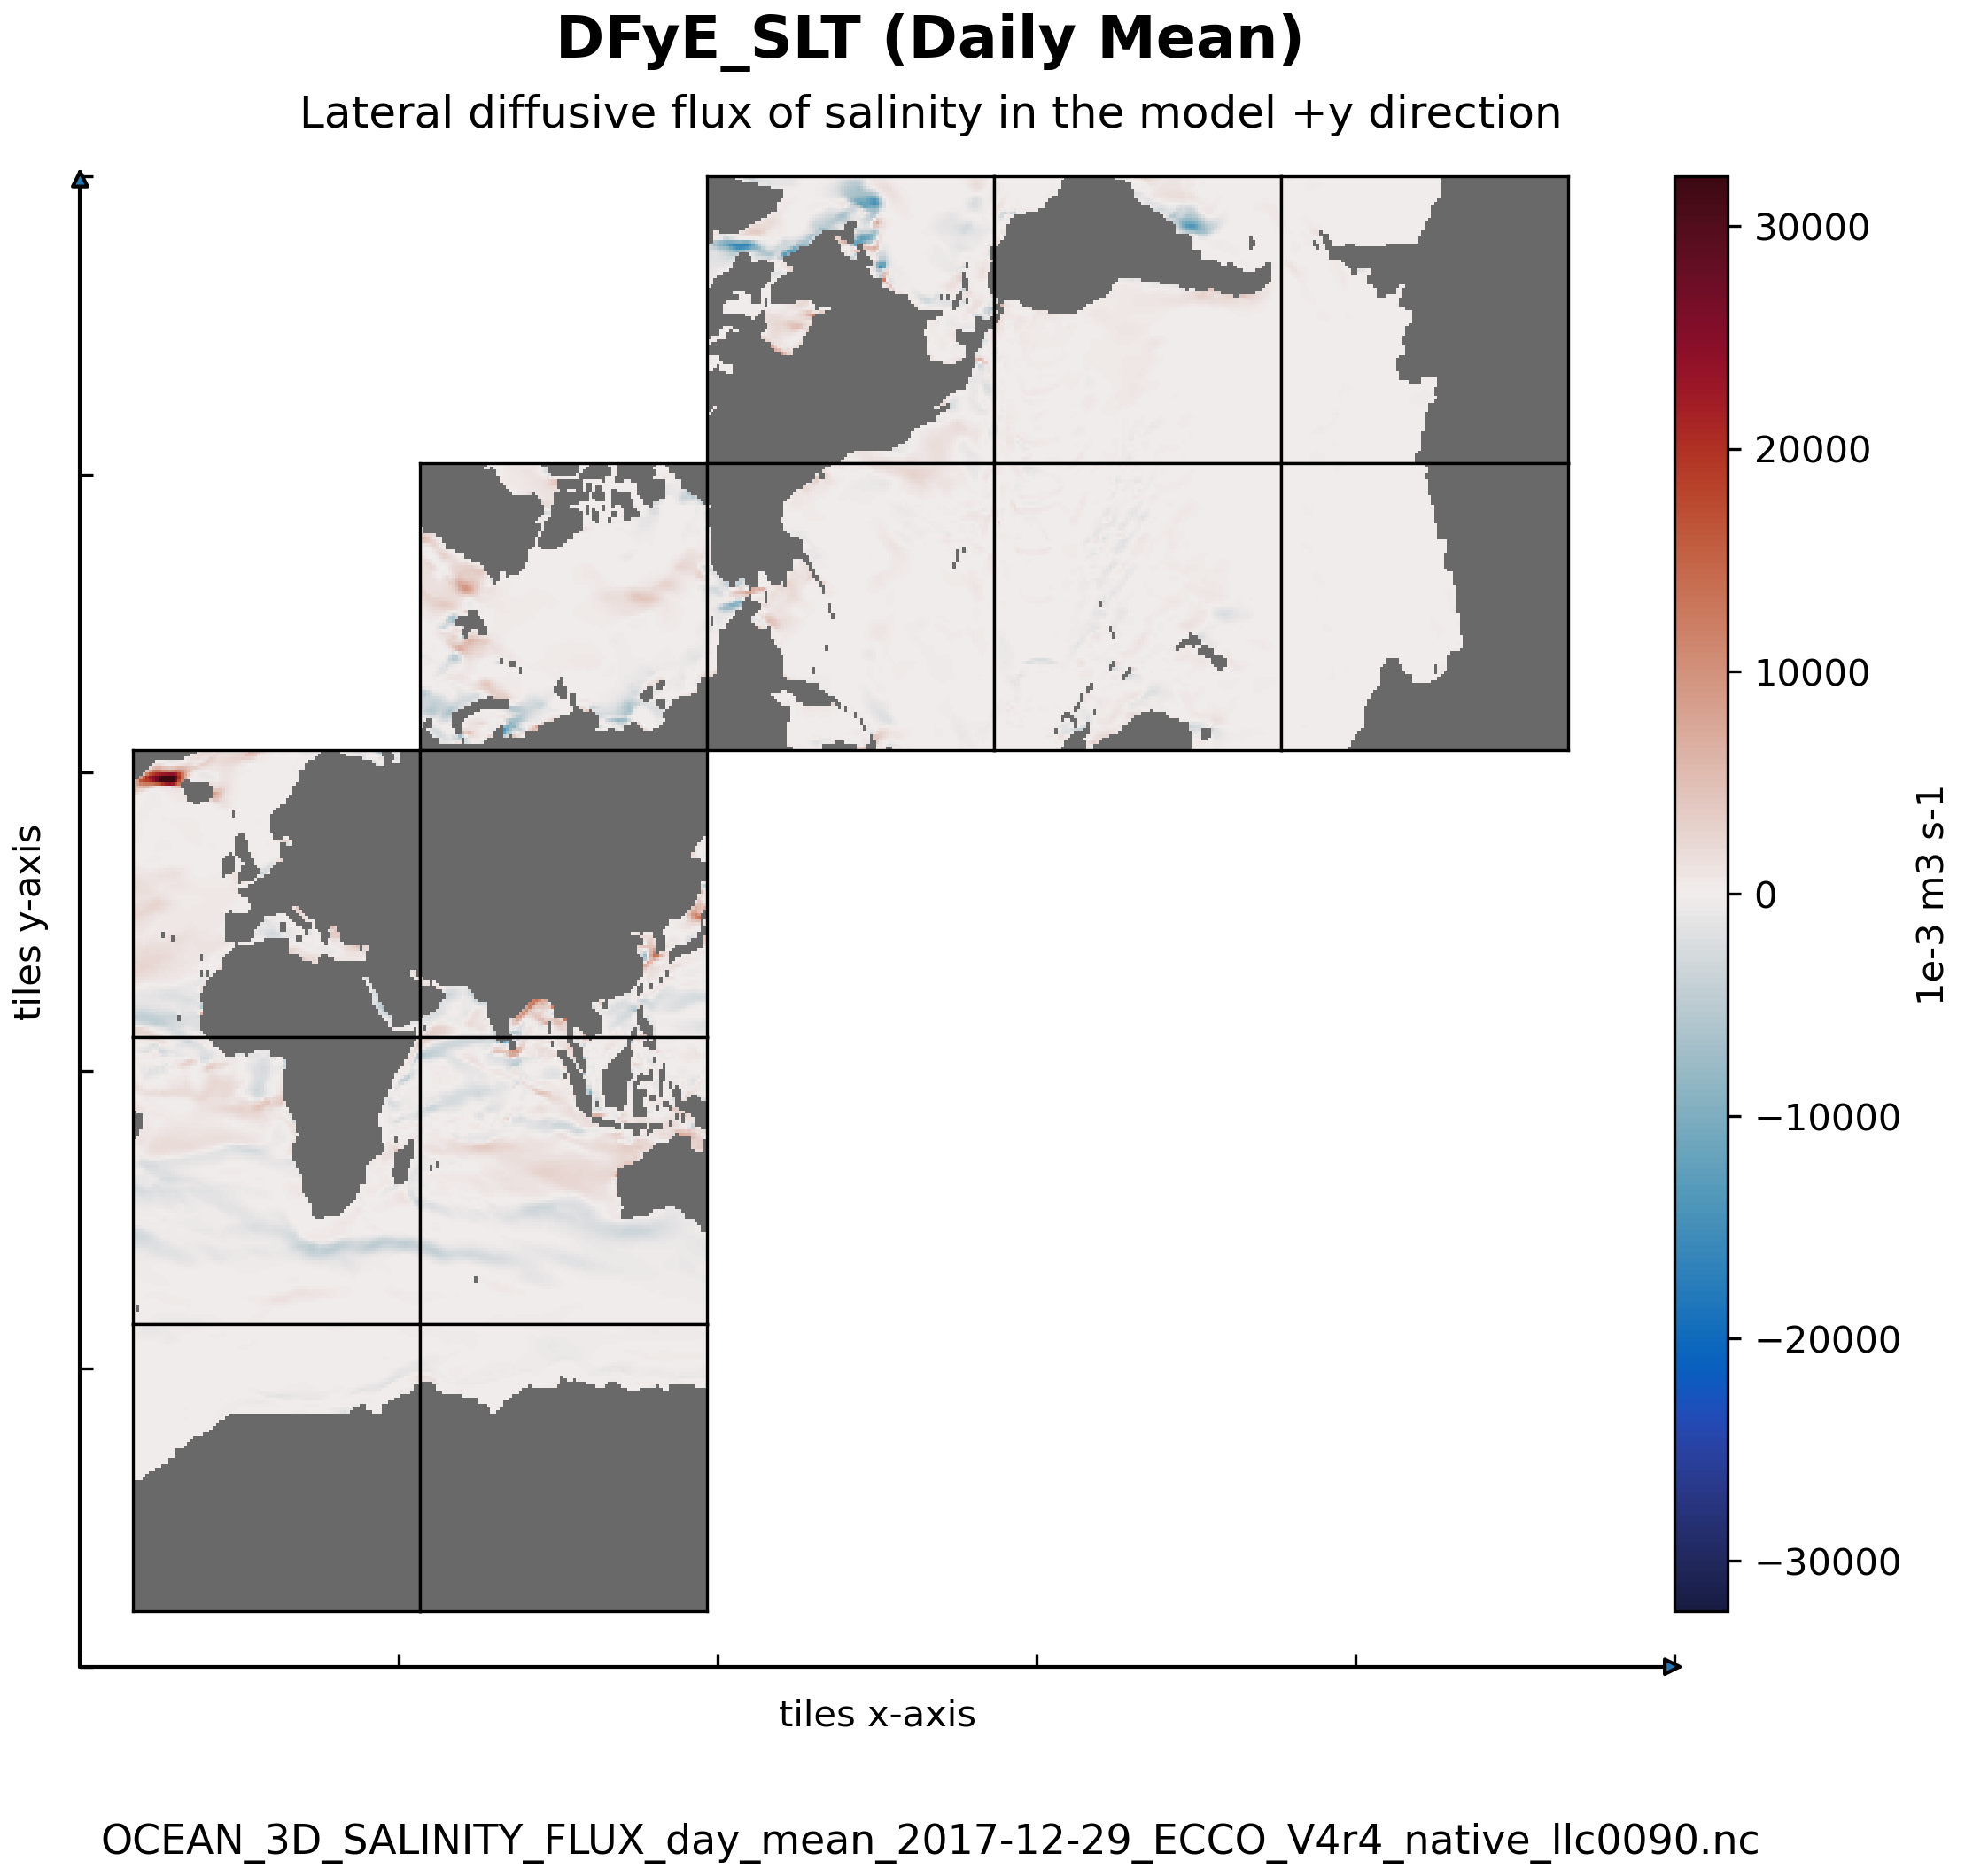
\includegraphics[scale=0.5]{../images/plots/native_plots/Ocean_Three-Dimensional_Salinity_Fluxes/DFyE_SLT.png}
\caption{\\Dataset: OCEAN\_3D\_SALINITY\_FLUX\\Variable: DFyE\_SLT}
\label{tab:table-OCEAN_3D_SALINITY_FLUX_DFyE_SLT-Plot}
\end{figure}
\pagebreak
\subsubsection{Native Variable oceSPtnd}
\begin{longtable}{|p{0.06\textwidth}|p{0.41\textwidth}|p{0.39\textwidth}|p{0.06\textwidth}|}
\caption{CDL description of OCEAN\_3D\_SALINITY\_FLUX's oceSPtnd variable}
\label{tab:table-OCEAN_3D_SALINITY_FLUX_oceSPtnd} \\ 
\hline \endhead \hline \endfoot
\rowcolor{lightgray} \textbf{Storage Type} & \textbf{Variable Name} & \textbf{Description} & \textbf{Unit} \\ \hline
float32 & oceSPtnd & Salt tendency due to the vertical transport of salt in high-salinity brine plumes & g m-2 s-1 \\ \hline
\rowcolor{lightgray}  \multicolumn{4}{|p{1.00\textwidth}|}{\textbf{CDL Description}} \\ \hline
\multicolumn{4}{|p{1.00\textwidth}|}{\makecell{\parbox{1\textwidth}{float32 oceSPtnd(time, k, tile, j, i)\\
\hspace*{0.5cm}oceSPtnd: \_FillValue = 9.96921e+36\\
\hspace*{0.5cm}oceSPtnd: long\_name = Salt tendency due to the vertical transport of salt in high: salinity brine plumes\\
\hspace*{0.5cm}oceSPtnd: units = g m: 2 s: 1\\
\hspace*{0.5cm}oceSPtnd: coverage\_content\_type = modelResult\\
\hspace*{0.5cm}oceSPtnd: direction = >0 increases salinity (SALT)\\
\hspace*{0.5cm}oceSPtnd: coordinates = XC Z YC time\\
\hspace*{0.5cm}oceSPtnd: valid\_min = 0.0\\
\hspace*{0.5cm}oceSPtnd: valid\_max = 0.021119138225913048}}} \\ \hline
\rowcolor{lightgray} \multicolumn{4}{|p{1.00\textwidth}|}{\textbf{Comments}} \\ \hline
\multicolumn{4}{|p{1\textwidth}|}{Salt tendency due to the vertical transport of salt in high-salinity brine plumes. Note: units are grams of salt per square meter per second, not salinity per square meter per second.} \\ \hline
\end{longtable}

\begin{figure}[H]
\centering
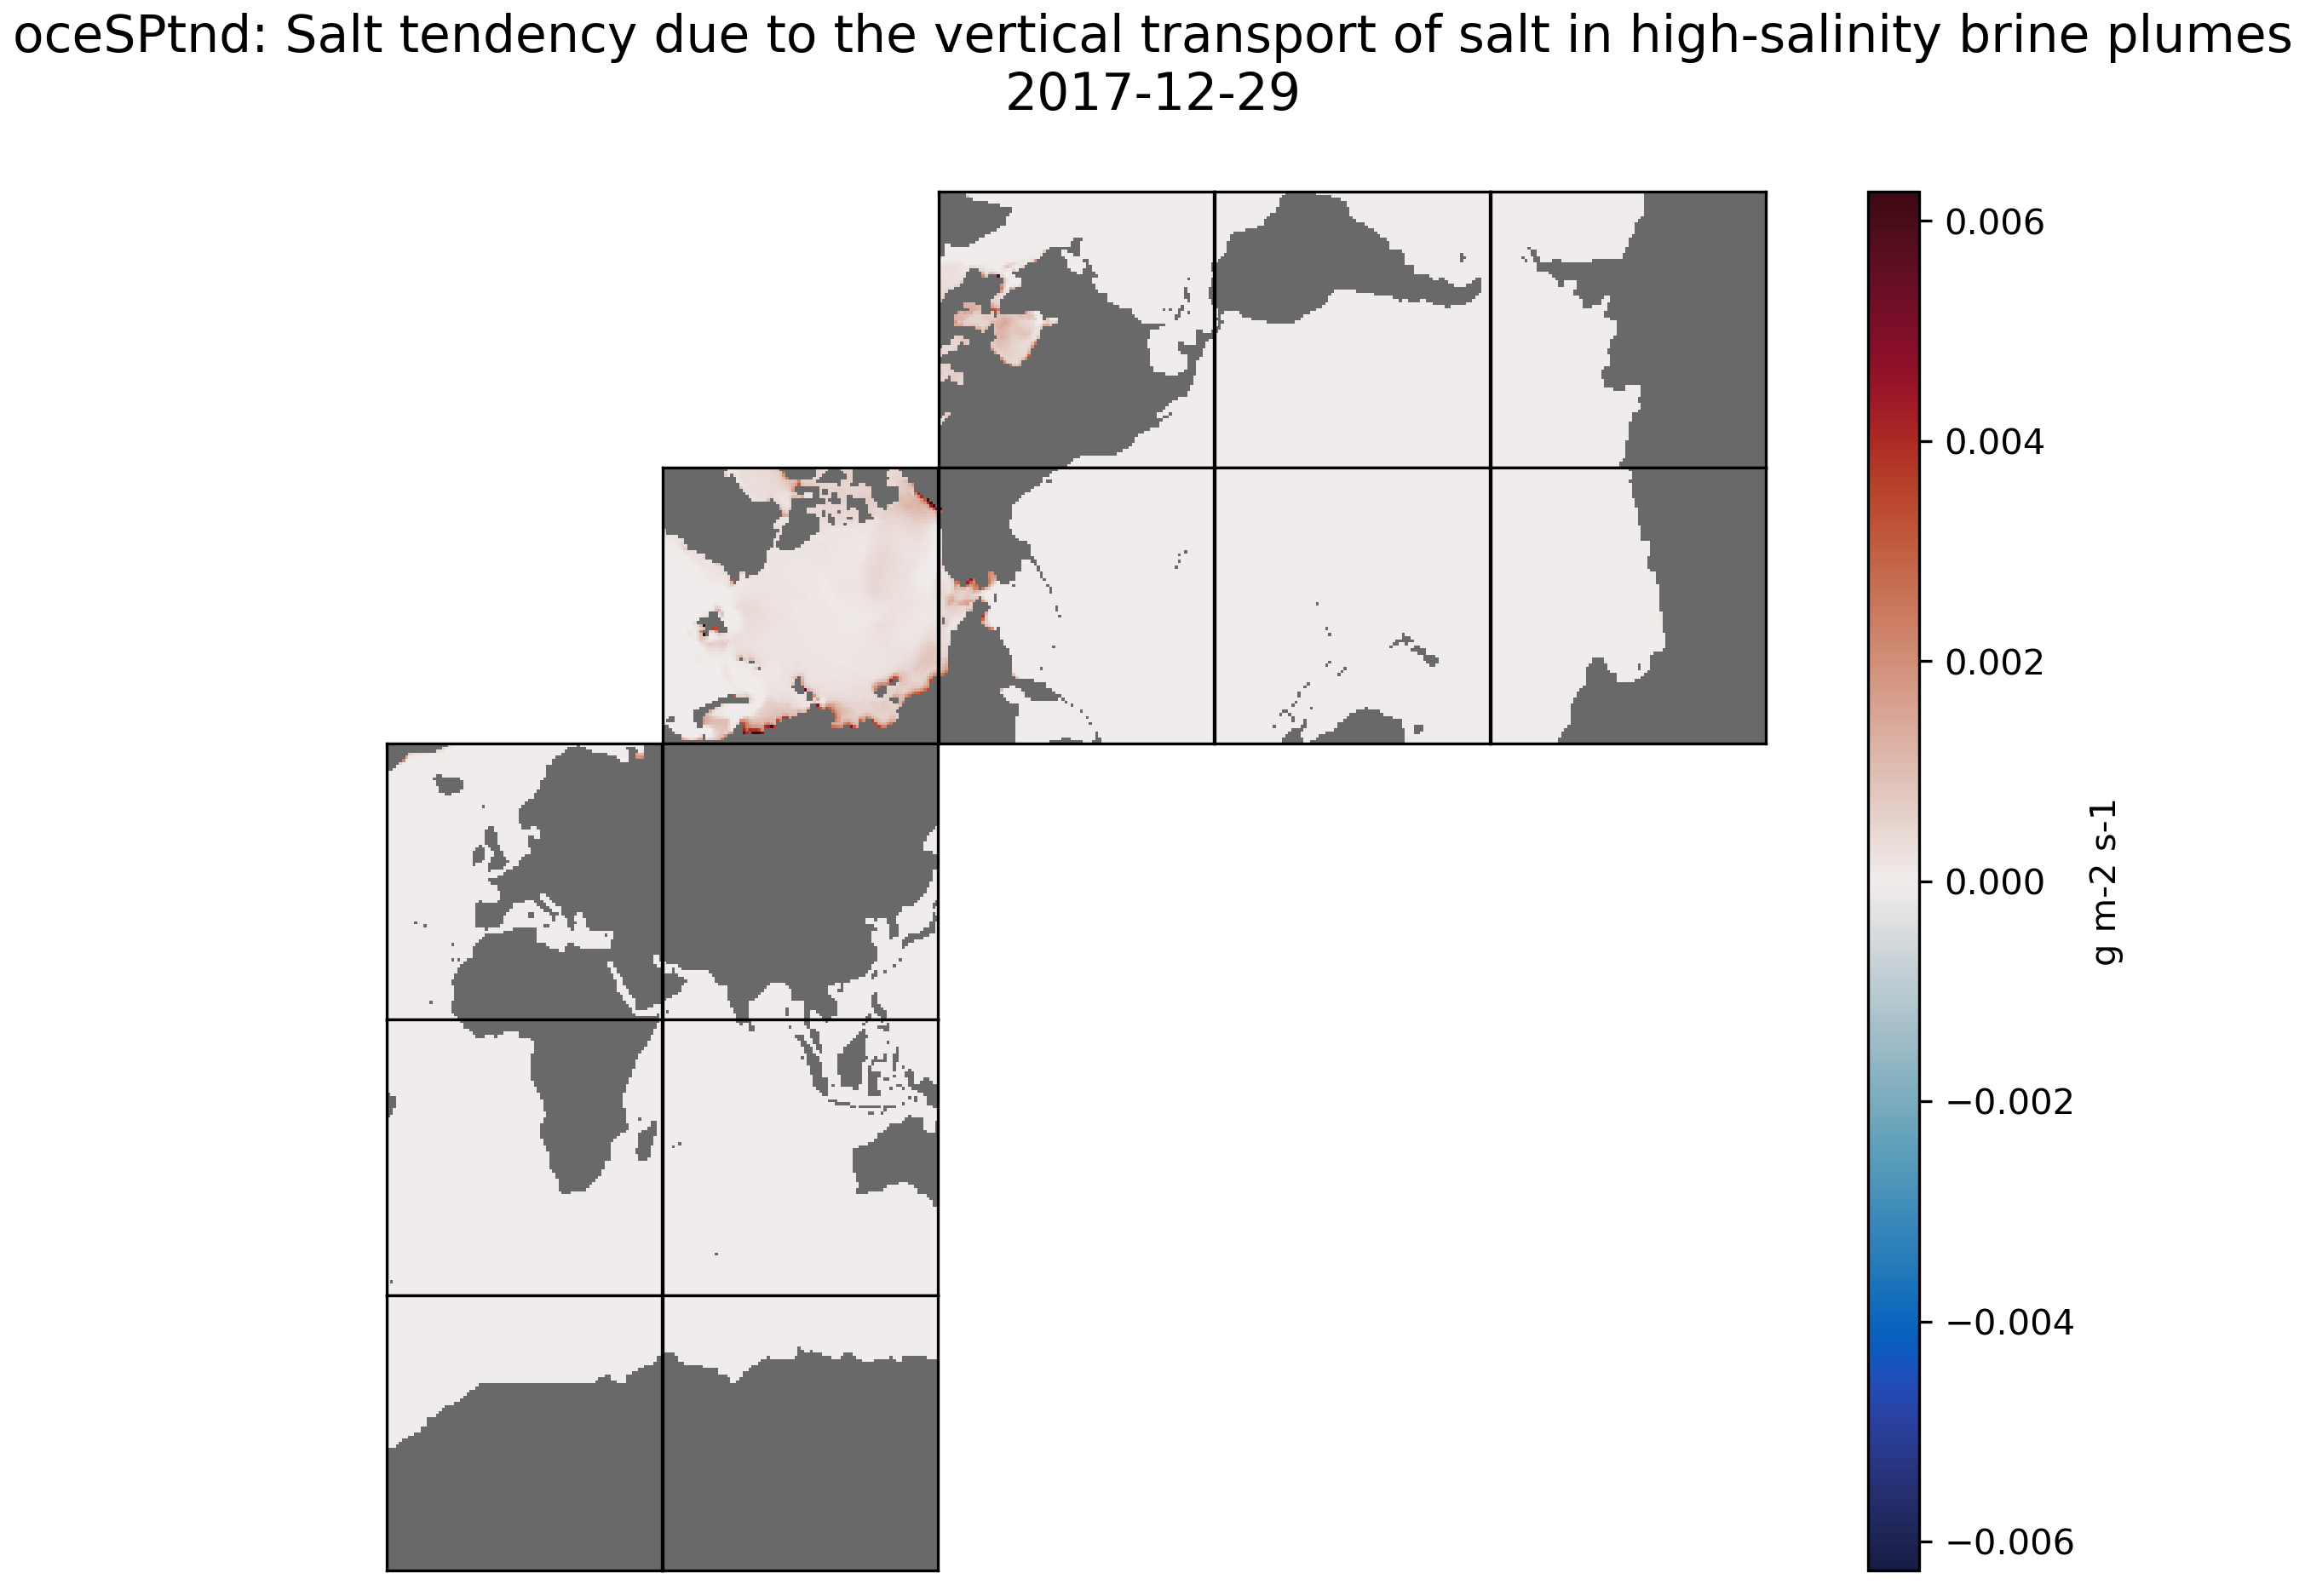
\includegraphics[scale=0.5]{../images/plots/native_plots/Ocean_Three-Dimensional_Salinity_Fluxes/oceSPtnd.png}
\caption{\\Dataset: OCEAN\_3D\_SALINITY\_FLUX\\Variable: oceSPtnd}
\label{tab:table-OCEAN_3D_SALINITY_FLUX_oceSPtnd-Plot}
\end{figure}
\pagebreak
\subsection{Native NetCDF OCEAN\_3D\_TEMPERATURE\_FLUX}
\newp
\begin{longtable}{|p{0.1\textwidth}|p{0.5\textwidth}|}
\caption{Variables in the dataset OCEAN\_3D\_TEMPERATURE\_FLUX}
\label{tab:table-OCEAN_3D_TEMPERATURE_FLUX-fields} \\ 
\hline \endhead \hline \endfoot
\rowcolor{lightgray} \textbf{Dataset:} & \textbf{OCEAN\_3D\_TEMPERATURE\_FLUX} \\ \hline
Field: &ADVx\_TH \\ \hline
Field: &DFxE\_TH \\ \hline
Field: &ADVy\_TH \\ \hline
Field: &DFyE\_TH \\ \hline
Field: &ADVr\_TH \\ \hline
Field: &DFrE\_TH \\ \hline
Field: &DFrI\_TH \\ \hline
\end{longtable}

\pagebreak
\subsubsection{Native Variable ADVr\_TH}
\begin{longtable}{|p{0.06\textwidth}|p{0.41\textwidth}|p{0.39\textwidth}|p{0.06\textwidth}|}
\caption{CDL description of OCEAN\_3D\_TEMPERATURE\_FLUX's ADVr\_TH variable}
\label{tab:table-OCEAN_3D_TEMPERATURE_FLUX_ADVr_TH} \\ 
\hline \endhead \hline \endfoot
\rowcolor{lightgray} \textbf{Storage Type} & \textbf{Variable Name} & \textbf{Description} & \textbf{Unit} \\ \hline
float32 & ADVr\_TH & Vertical advective flux of potential temperature & degree\_C m3 s-1 \\ \hline
\rowcolor{lightgray}  \multicolumn{4}{|p{1.00\textwidth}|}{\textbf{CDL Description}} \\ \hline
\multicolumn{4}{|p{1.00\textwidth}|}{\makecell{\parbox{1\textwidth}{float32 ADVr\_TH(time, k\_l, tile, j, i)\\
\hspace*{0.5cm}ADVr\_TH: \_FillValue = 9.96921e+36\\
\hspace*{0.5cm}ADVr\_TH: long\_name = Vertical advective flux of potential temperature\\
\hspace*{0.5cm}ADVr\_TH: units = degree\_C m3 s: 1\\
\hspace*{0.5cm}ADVr\_TH: coverage\_content\_type = modelResult\\
\hspace*{0.5cm}ADVr\_TH: direction = >0 decreases potential temperature (THETA)\\
\hspace*{0.5cm}ADVr\_TH: coordinates = XC YC time Zl\\
\hspace*{0.5cm}ADVr\_TH: valid\_min = : 125094904.0\\
\hspace*{0.5cm}ADVr\_TH: valid\_max = 179459344.0}}} \\ \hline
\rowcolor{lightgray} \multicolumn{4}{|p{1.00\textwidth}|}{\textbf{Comments}} \\ \hline
\multicolumn{4}{|p{1\textwidth}|}{Vertical advective flux of potential temperature (THETA) in the +z direction through the top 'w' face of the tracer cell on the native model grid. Note: in the Arakawa-C grid, vertical flux quantities are staggered relative to the tracer cells with indexing such that +ADVr\_TH(i,j,k\_l) corresponds to upward +z fluxes through the top 'w' face of the tracer cell at (i,j,k)} \\ \hline
\end{longtable}

\begin{figure}[H]
\centering
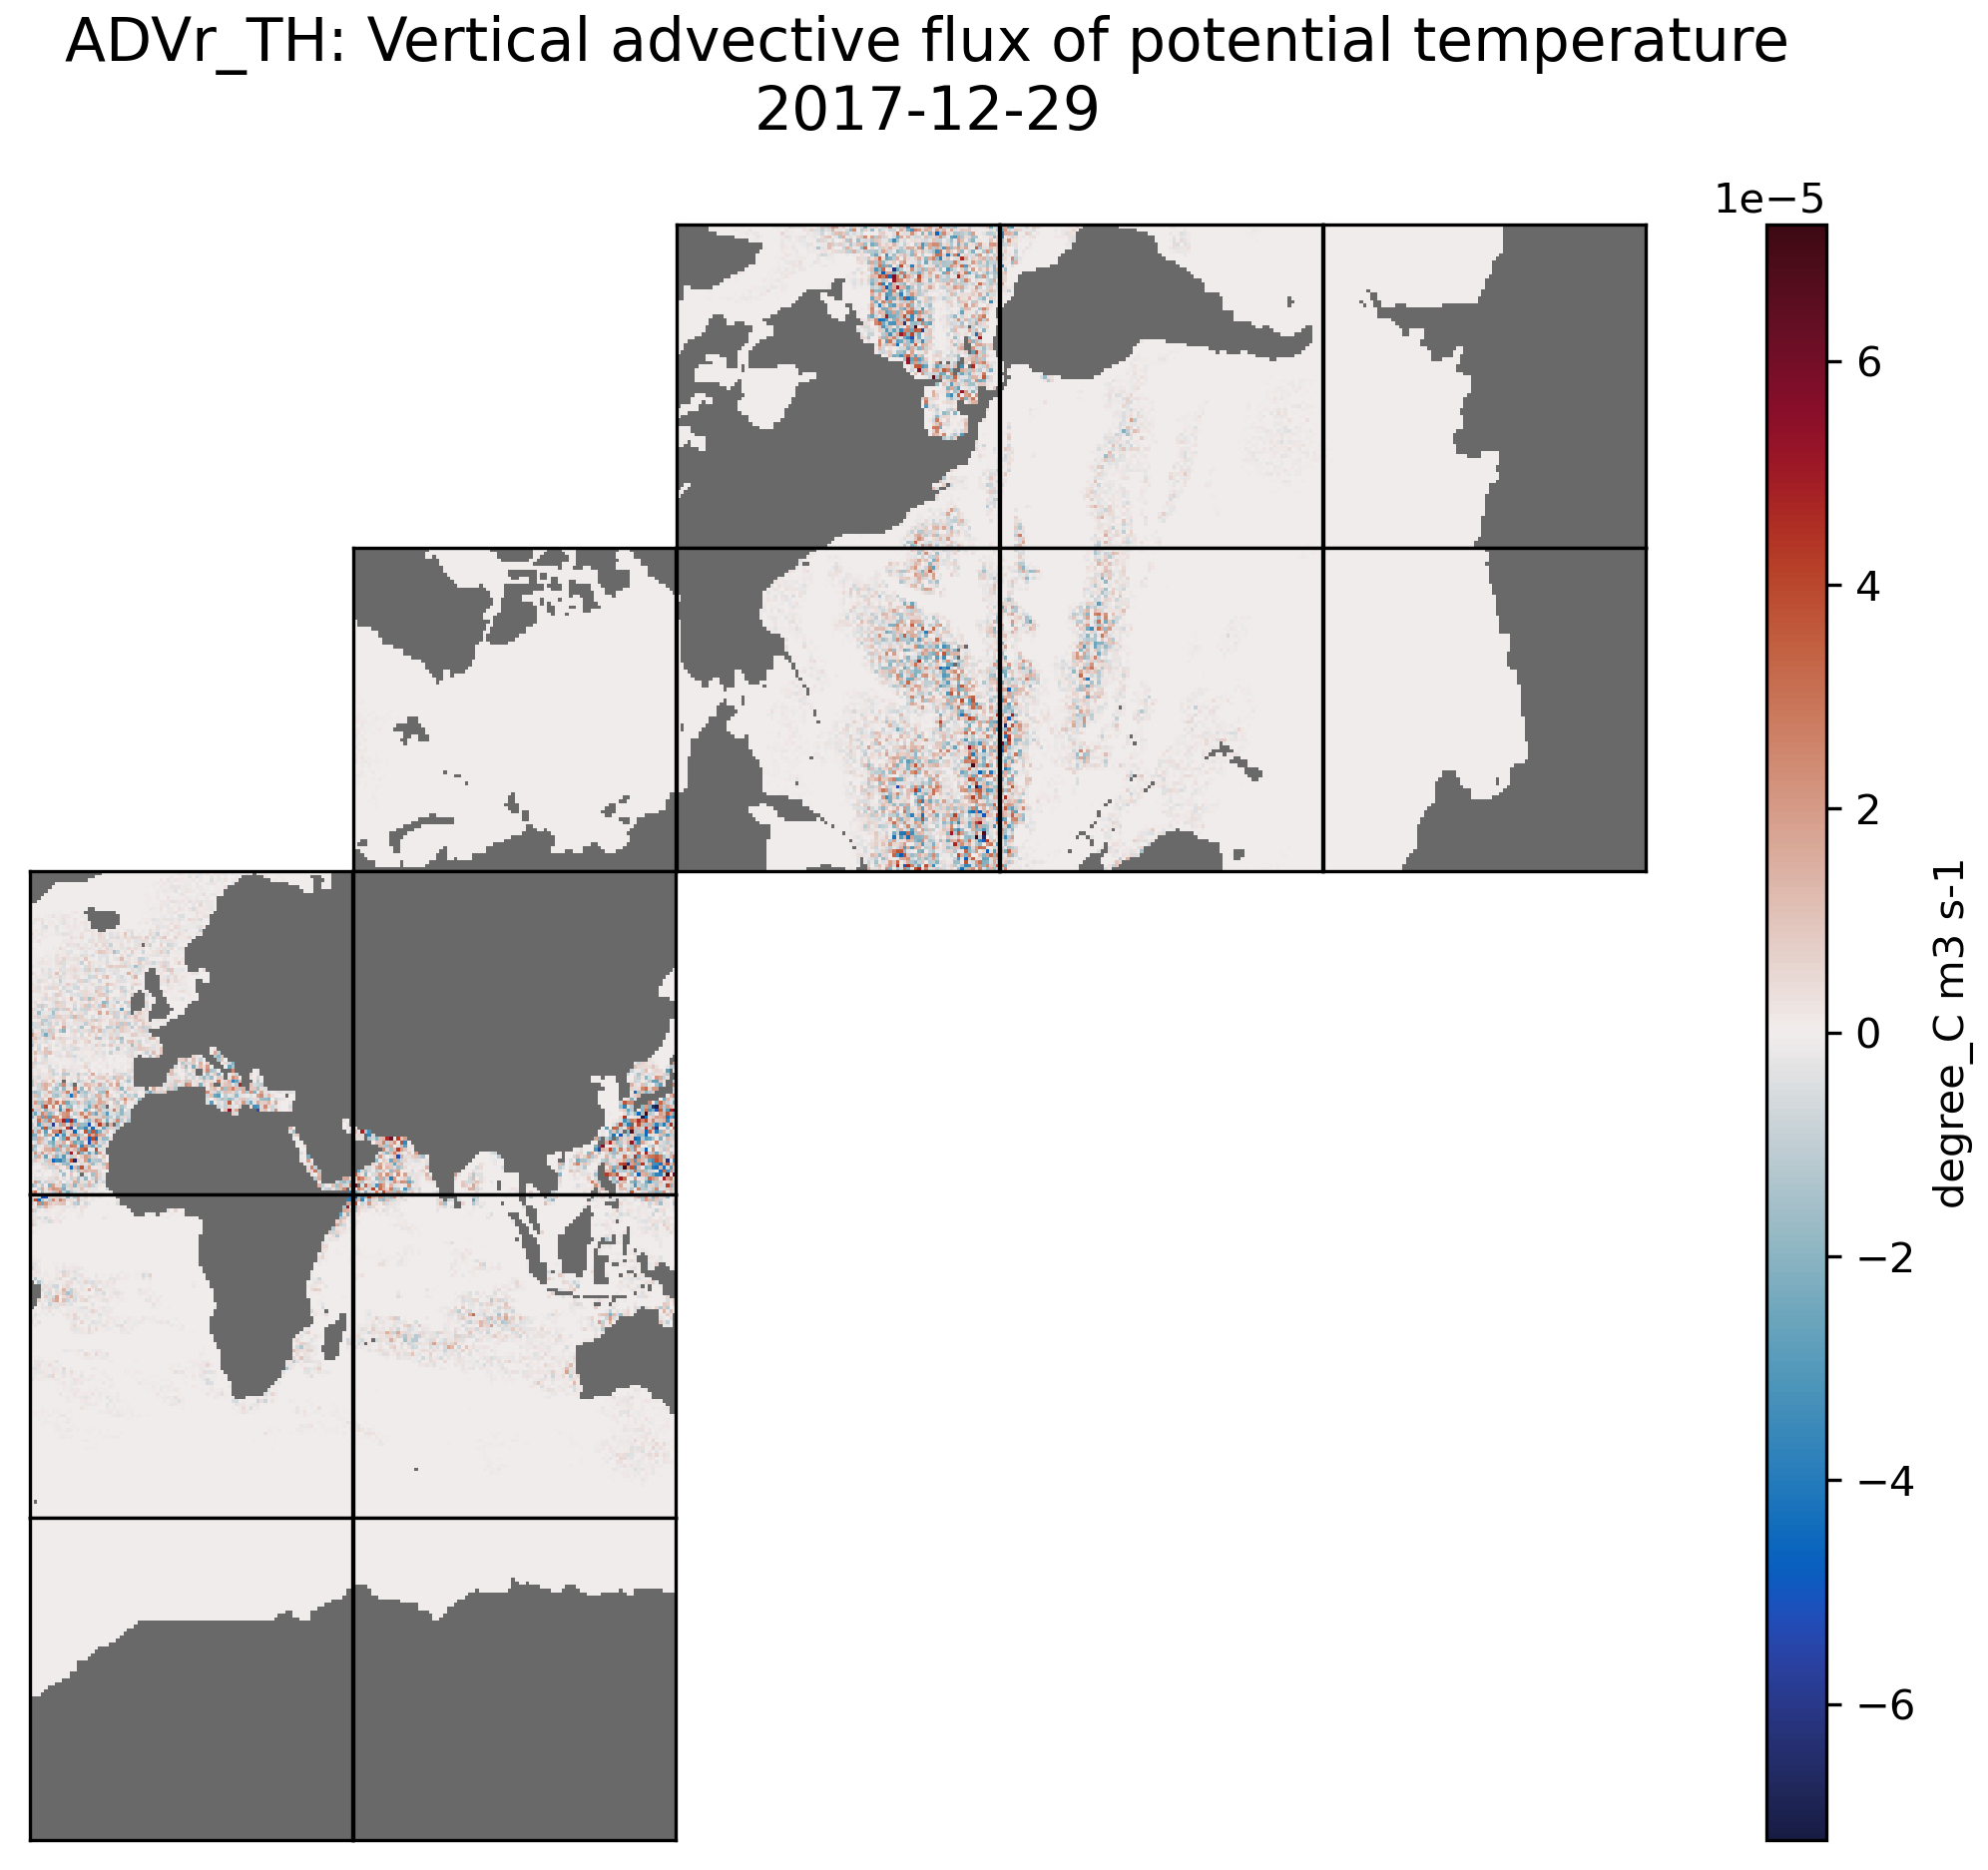
\includegraphics[scale=0.5]{../images/plots/native_plots/Ocean_Three-Dimensional_Potential_Temperature_Fluxes/ADVr_TH.png}
\caption{\\Dataset: OCEAN\_3D\_TEMPERATURE\_FLUX\\Variable: ADVr\_TH}
\label{tab:table-OCEAN_3D_TEMPERATURE_FLUX_ADVr_TH-Plot}
\end{figure}
\pagebreak
\subsubsection{Native Variable ADVx\_TH}
\begin{longtable}{|p{0.06\textwidth}|p{0.41\textwidth}|p{0.39\textwidth}|p{0.06\textwidth}|}
\caption{CDL description of OCEAN\_3D\_TEMPERATURE\_FLUX's ADVx\_TH variable}
\label{tab:table-OCEAN_3D_TEMPERATURE_FLUX_ADVx_TH} \\ 
\hline \endhead \hline \endfoot
\rowcolor{lightgray} \textbf{Storage Type} & \textbf{Variable Name} & \textbf{Description} & \textbf{Unit} \\ \hline
float32 & ADVx\_TH & Lateral advective flux of potential temperature in the model +x direction & degree\_C m3 s-1 \\ \hline
\rowcolor{lightgray}  \multicolumn{4}{|p{1.00\textwidth}|}{\textbf{CDL Description}} \\ \hline
\multicolumn{4}{|p{1.00\textwidth}|}{\makecell{\parbox{1\textwidth}{float32 ADVx\_TH(time, k, tile, j, i\_g)\\
\hspace*{0.5cm}ADVx\_TH: \_FillValue = 9.96921e+36\\
\hspace*{0.5cm}ADVx\_TH: long\_name = Lateral advective flux of potential temperature in the model +x direction\\
\hspace*{0.5cm}ADVx\_TH: units = degree\_C m3 s: 1\\
\hspace*{0.5cm}ADVx\_TH: mate = ADVy\_TH\\
\hspace*{0.5cm}ADVx\_TH: coverage\_content\_type = modelResult\\
\hspace*{0.5cm}ADVx\_TH: direction = >0 increases potential temperature (THETA)\\
\hspace*{0.5cm}ADVx\_TH: coordinates = time Z\\
\hspace*{0.5cm}ADVx\_TH: valid\_min = : 38210700.0\\
\hspace*{0.5cm}ADVx\_TH: valid\_max = 38049636.0}}} \\ \hline
\rowcolor{lightgray} \multicolumn{4}{|p{1.00\textwidth}|}{\textbf{Comments}} \\ \hline
\multicolumn{4}{|p{1\textwidth}|}{Lateral advective flux of potential temperature (THETA) in the +x direction through the 'u' face of the tracer cell on the native model grid. Note: in the Arakawa-C grid, horizontal flux quantities are staggered relative to the tracer cells with indexing such that +ADVx\_TH(i\_g,j,k) corresponds to +x fluxes through the 'u' face of the tracer cell at (i,j,k). Also, the model +x direction does not necessarily correspond to the geographical east-west direction because the x and y axes of the model's lat-lon-cap (llc) curvilinear lat-lon-cap (llc) grid have arbitrary orientations which vary within and across tiles.} \\ \hline
\end{longtable}

\begin{figure}[H]
\centering
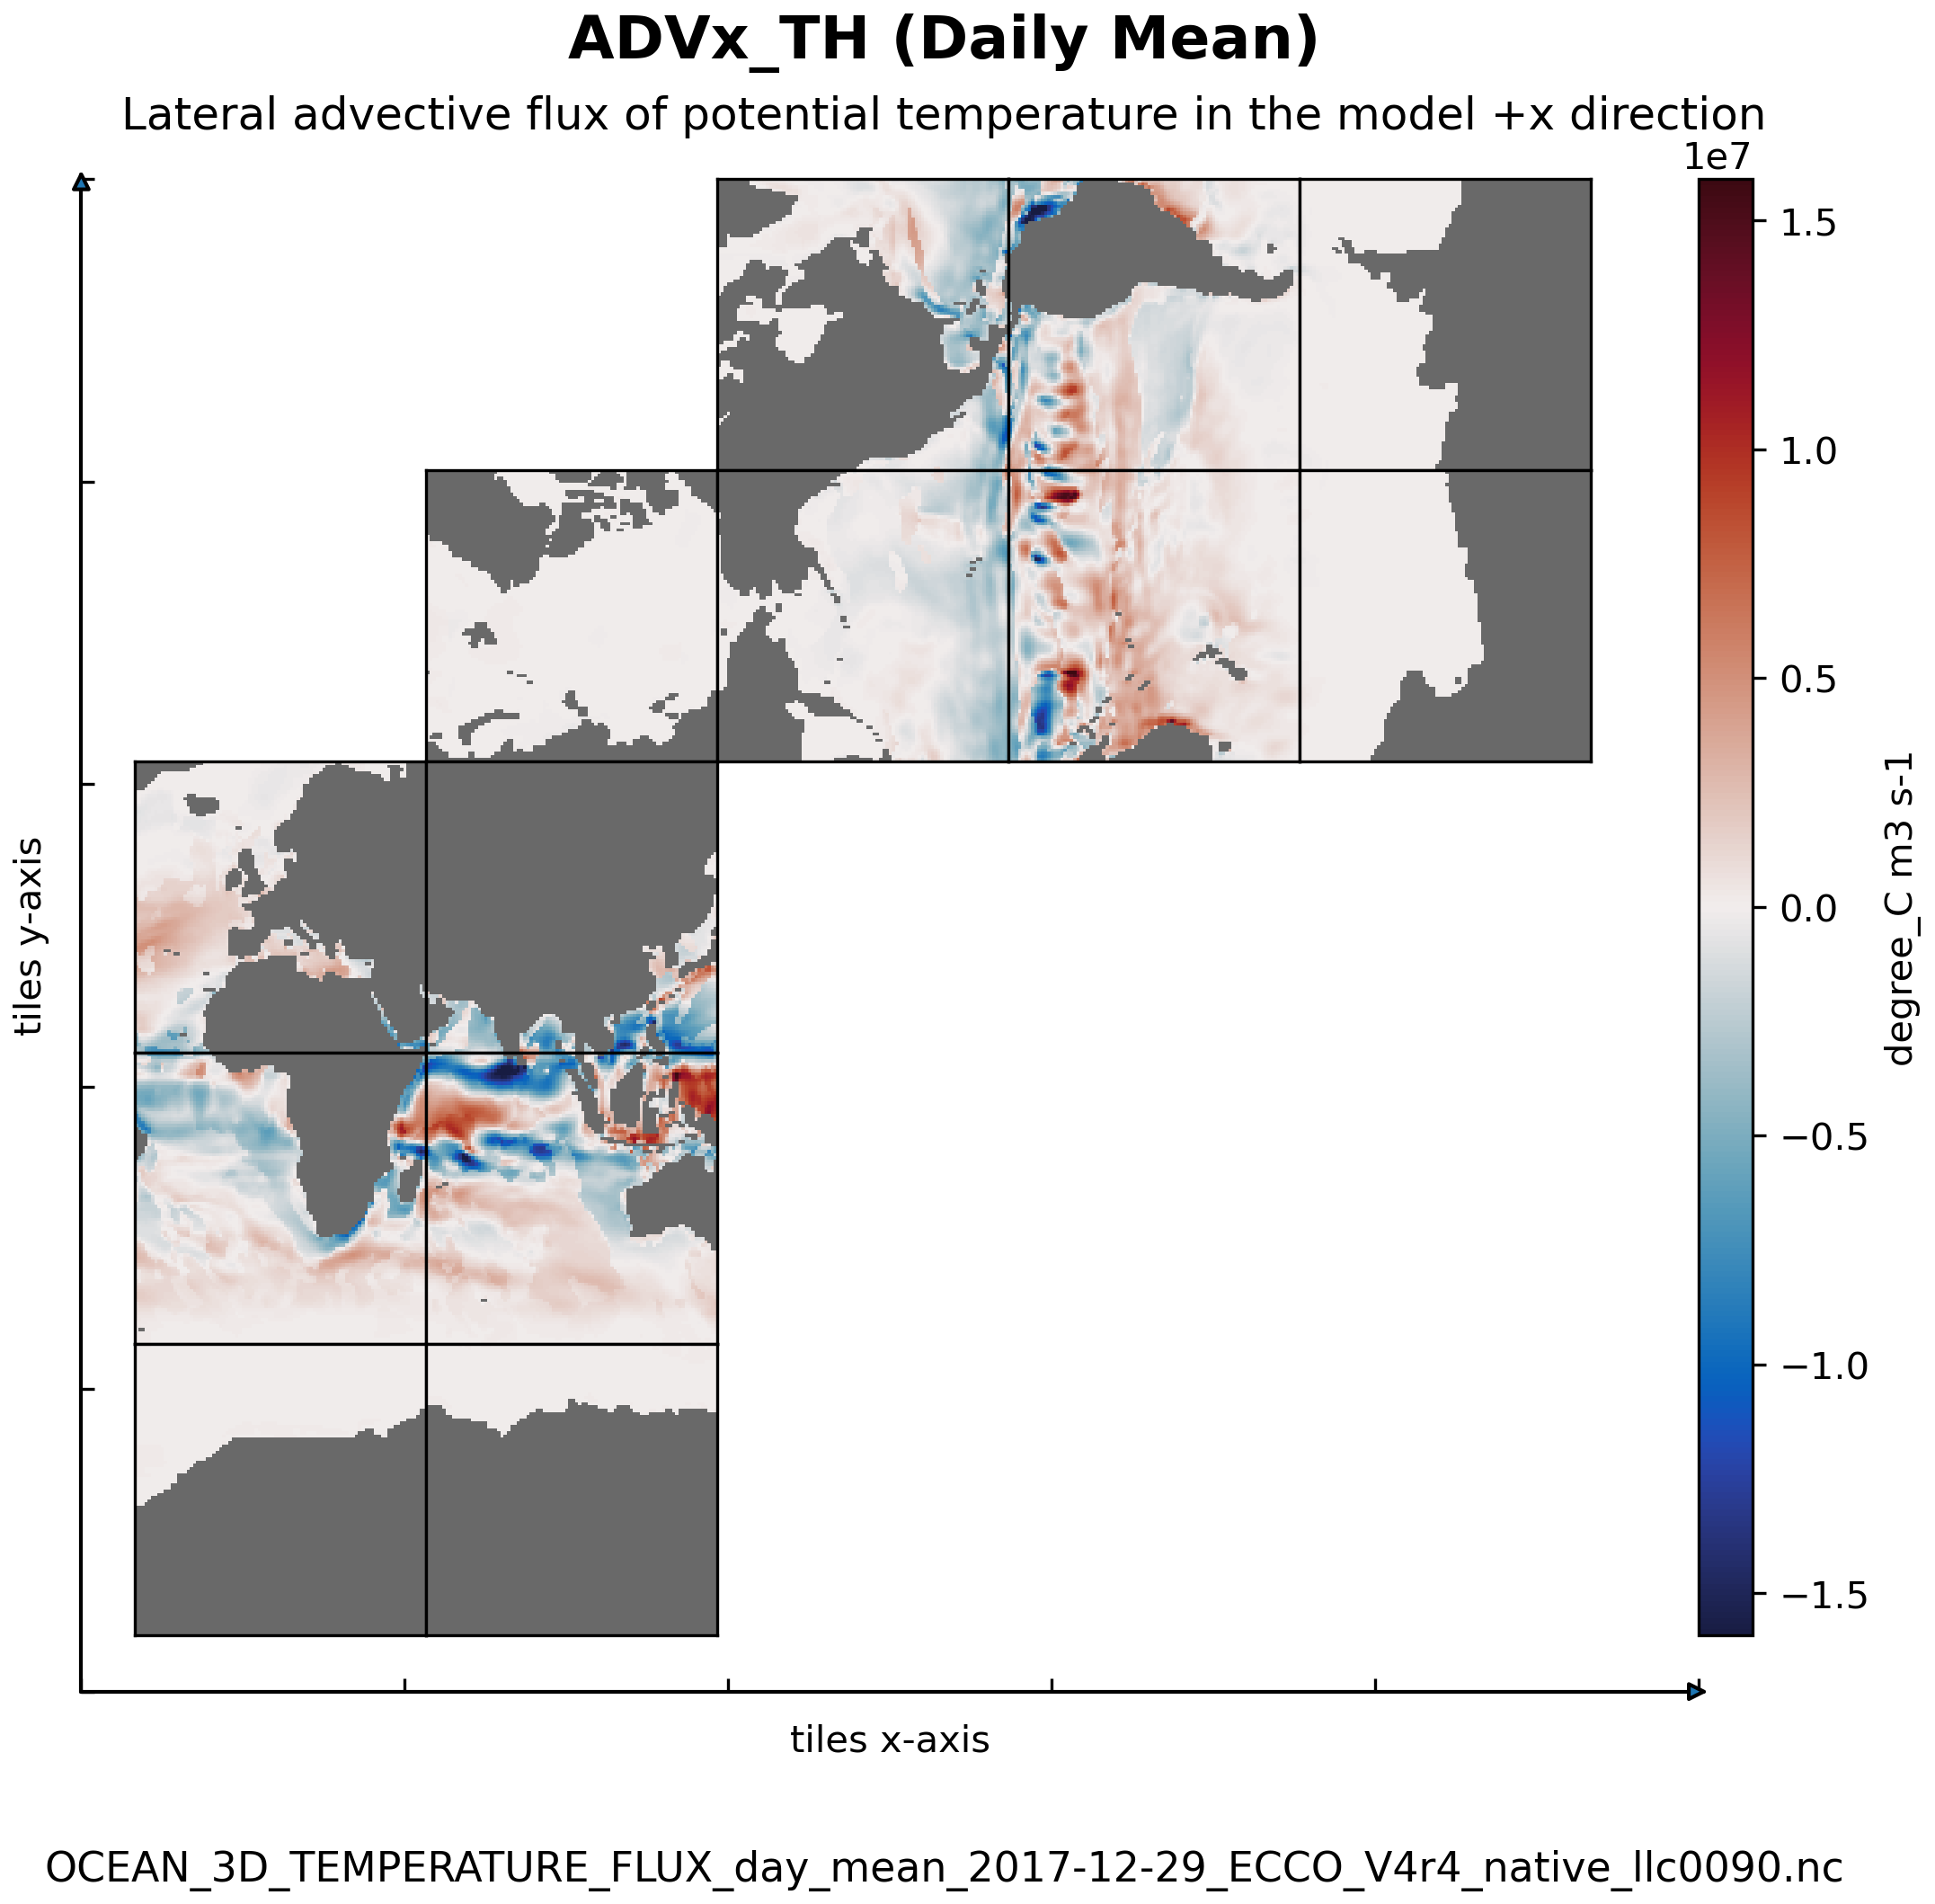
\includegraphics[scale=0.5]{../images/plots/native_plots/Ocean_Three-Dimensional_Potential_Temperature_Fluxes/ADVx_TH.png}
\caption{\\Dataset: OCEAN\_3D\_TEMPERATURE\_FLUX\\Variable: ADVx\_TH}
\label{tab:table-OCEAN_3D_TEMPERATURE_FLUX_ADVx_TH-Plot}
\end{figure}
\pagebreak
\subsubsection{Native Variable ADVy\_TH}
\begin{longtable}{|p{0.06\textwidth}|p{0.41\textwidth}|p{0.39\textwidth}|p{0.06\textwidth}|}
\caption{CDL description of OCEAN\_3D\_TEMPERATURE\_FLUX's ADVy\_TH variable}
\label{tab:table-OCEAN_3D_TEMPERATURE_FLUX_ADVy_TH} \\ 
\hline \endhead \hline \endfoot
\rowcolor{lightgray} \textbf{Storage Type} & \textbf{Variable Name} & \textbf{Description} & \textbf{Unit} \\ \hline
float32 & ADVy\_TH & Lateral advective flux of potential temperature in the model +y direction & degree\_C m3 s-1 \\ \hline
\rowcolor{lightgray}  \multicolumn{4}{|p{1.00\textwidth}|}{\textbf{CDL Description}} \\ \hline
\multicolumn{4}{|p{1.00\textwidth}|}{\makecell{\parbox{1\textwidth}{float32 ADVy\_TH(time, k, tile, j\_g, i)\\
\hspace*{0.5cm}ADVy\_TH: \_FillValue = 9.96921e+36\\
\hspace*{0.5cm}ADVy\_TH: long\_name = Lateral advective flux of potential temperature in the model +y direction\\
\hspace*{0.5cm}ADVy\_TH: units = degree\_C m3 s: 1\\
\hspace*{0.5cm}ADVy\_TH: mate = ADVx\_TH\\
\hspace*{0.5cm}ADVy\_TH: coverage\_content\_type = modelResult\\
\hspace*{0.5cm}ADVy\_TH: direction = >0 increases potential temperature (THETA)\\
\hspace*{0.5cm}ADVy\_TH: coordinates = time Z\\
\hspace*{0.5cm}ADVy\_TH: valid\_min = : 43909120.0\\
\hspace*{0.5cm}ADVy\_TH: valid\_max = 56347884.0}}} \\ \hline
\rowcolor{lightgray} \multicolumn{4}{|p{1.00\textwidth}|}{\textbf{Comments}} \\ \hline
\multicolumn{4}{|p{1\textwidth}|}{Lateral advective flux of potential temperature (THETA) in the +y direction through the 'v' face of the tracer cell on the native model grid. Note: in the Arakawa-C grid, horizontal flux quantities are staggered relative to the tracer cells with indexing such that +ADVy\_TH(i,j\_g,k) corresponds to +y fluxes through the 'v' face of the tracer cell at (i,j,k). Also, the model +y direction does not necessarily correspond to the geographical north-south direction because the x and y axes of the model's curvilinear lat-lon-cap (llc) grid have arbitrary orientations which vary within and across tiles.} \\ \hline
\end{longtable}

\begin{figure}[H]
\centering
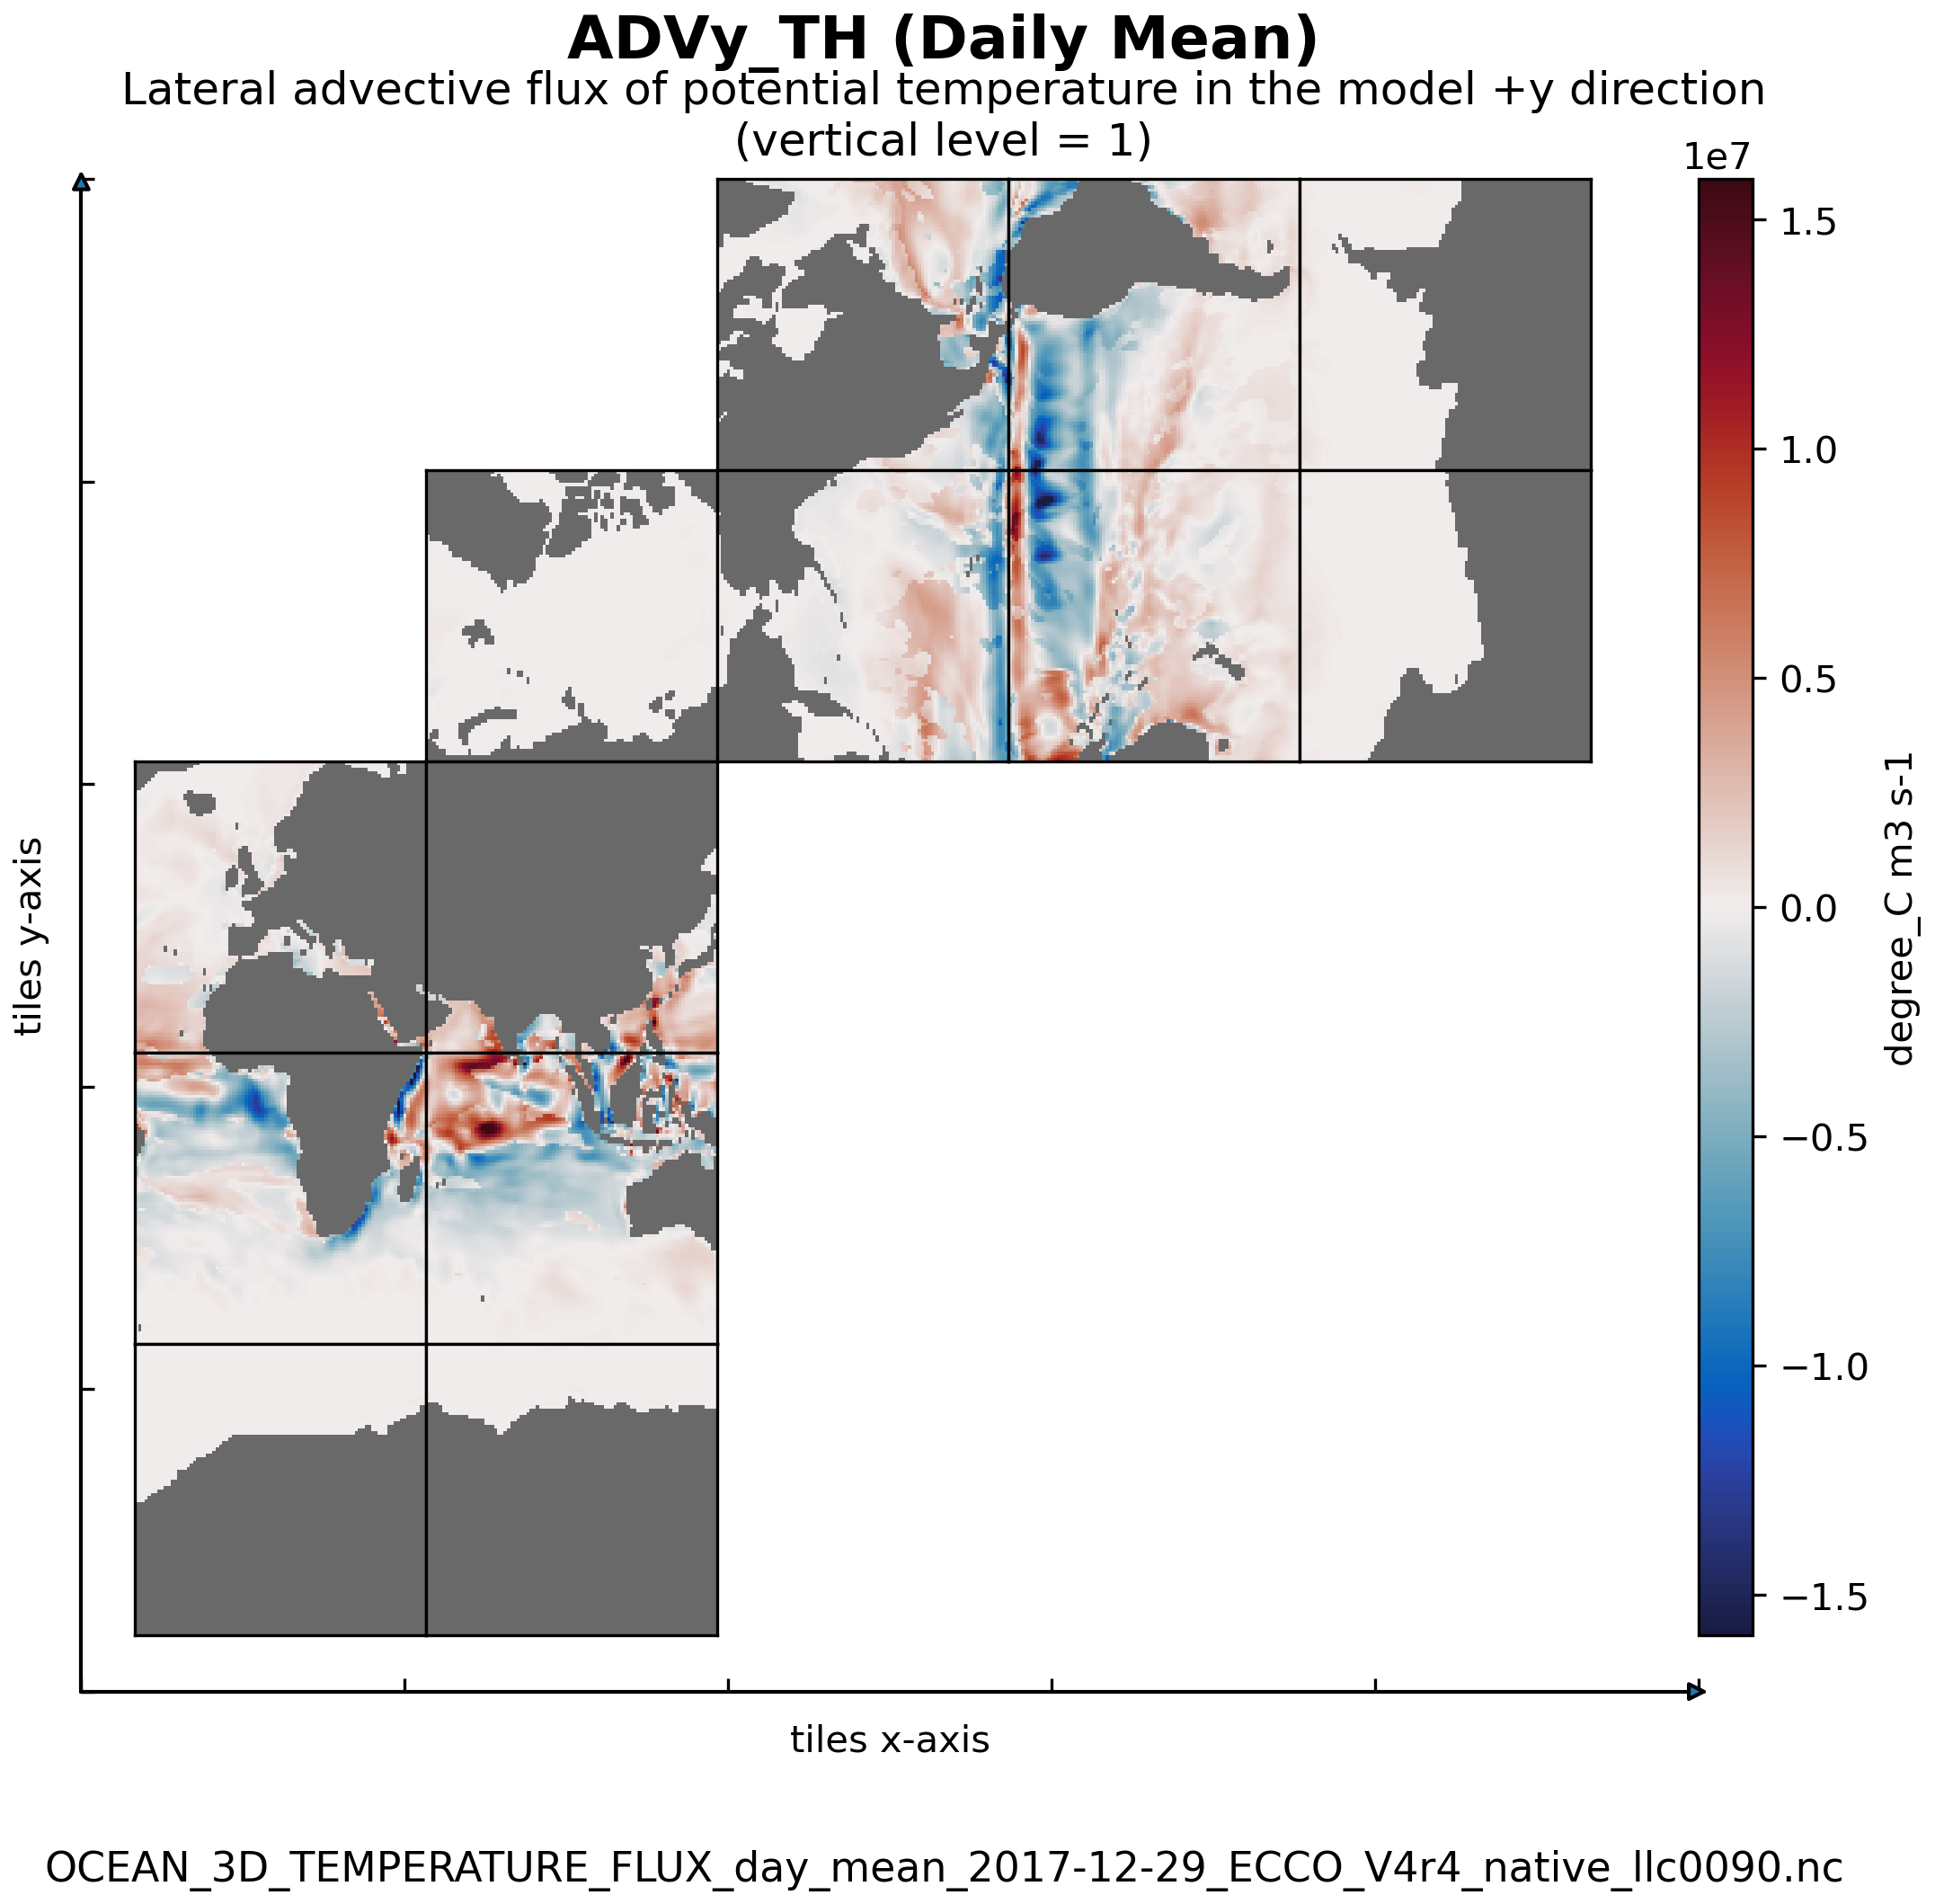
\includegraphics[scale=0.5]{../images/plots/native_plots/Ocean_Three-Dimensional_Potential_Temperature_Fluxes/ADVy_TH.png}
\caption{\\Dataset: OCEAN\_3D\_TEMPERATURE\_FLUX\\Variable: ADVy\_TH}
\label{tab:table-OCEAN_3D_TEMPERATURE_FLUX_ADVy_TH-Plot}
\end{figure}
\pagebreak
\subsubsection{Native Variable DFrE\_TH}
\begin{longtable}{|p{0.06\textwidth}|p{0.41\textwidth}|p{0.39\textwidth}|p{0.06\textwidth}|}
\caption{CDL description of OCEAN\_3D\_TEMPERATURE\_FLUX's DFrE\_TH variable}
\label{tab:table-OCEAN_3D_TEMPERATURE_FLUX_DFrE_TH} \\ 
\hline \endhead \hline \endfoot
\rowcolor{lightgray} \textbf{Storage Type} & \textbf{Variable Name} & \textbf{Description} & \textbf{Unit} \\ \hline
float32 & DFrE\_TH & Vertical diffusive flux of potential temperature (explicit term) & degree\_C m3 s-1 \\ \hline
\rowcolor{lightgray}  \multicolumn{4}{|p{1.00\textwidth}|}{\textbf{CDL Description}} \\ \hline
\multicolumn{4}{|p{1.00\textwidth}|}{\makecell{\parbox{1\textwidth}{float32 DFrE\_TH(time, k\_l, tile, j, i)\\
\hspace*{0.5cm}DFrE\_TH: \_FillValue = 9.96921e+36\\
\hspace*{0.5cm}DFrE\_TH: long\_name = Vertical diffusive flux of potential temperature (explicit term)\\
\hspace*{0.5cm}DFrE\_TH: units = degree\_C m3 s: 1\\
\hspace*{0.5cm}DFrE\_TH: coverage\_content\_type = modelResult\\
\hspace*{0.5cm}DFrE\_TH: direction = >0 decreases potential temperature (THETA)\\
\hspace*{0.5cm}DFrE\_TH: coordinates = XC YC time Zl\\
\hspace*{0.5cm}DFrE\_TH: valid\_min = : 2632379.75\\
\hspace*{0.5cm}DFrE\_TH: valid\_max = 2659875.25}}} \\ \hline
\rowcolor{lightgray} \multicolumn{4}{|p{1.00\textwidth}|}{\textbf{Comments}} \\ \hline
\multicolumn{4}{|p{1\textwidth}|}{The explicit term of the vertical diffusive flux of potential temperature (THETA) in the +z direction through the top 'w' face of the tracer cell on the native model grid. In the ECCO V4r4 model, an implicit scheme is used to calculate vertical diffusive tracer fluxes due to background diffusivity and the Kwz component of the GM-Redi tensor (vertical flux as a function of vertical gradient) while an explicit scheme is used to calculate the vertical diffusive fluxes from the Kwx and Kwy components of the GM-Redi tensor (vertical flux as a function of horizontal gradient). Both implicit and explicit components of vertical diffusive flux of potential temperature are provided. Note: in the Arakawa-C grid, vertical flux quantities are staggered relative to the tracer cells with indexing such that +DFrE\_TH(i,j,k\_l) corresponds to upward +z fluxes through the top 'w' face of the tracer cell at (i,j,k).} \\ \hline
\end{longtable}

\begin{figure}[H]
\centering
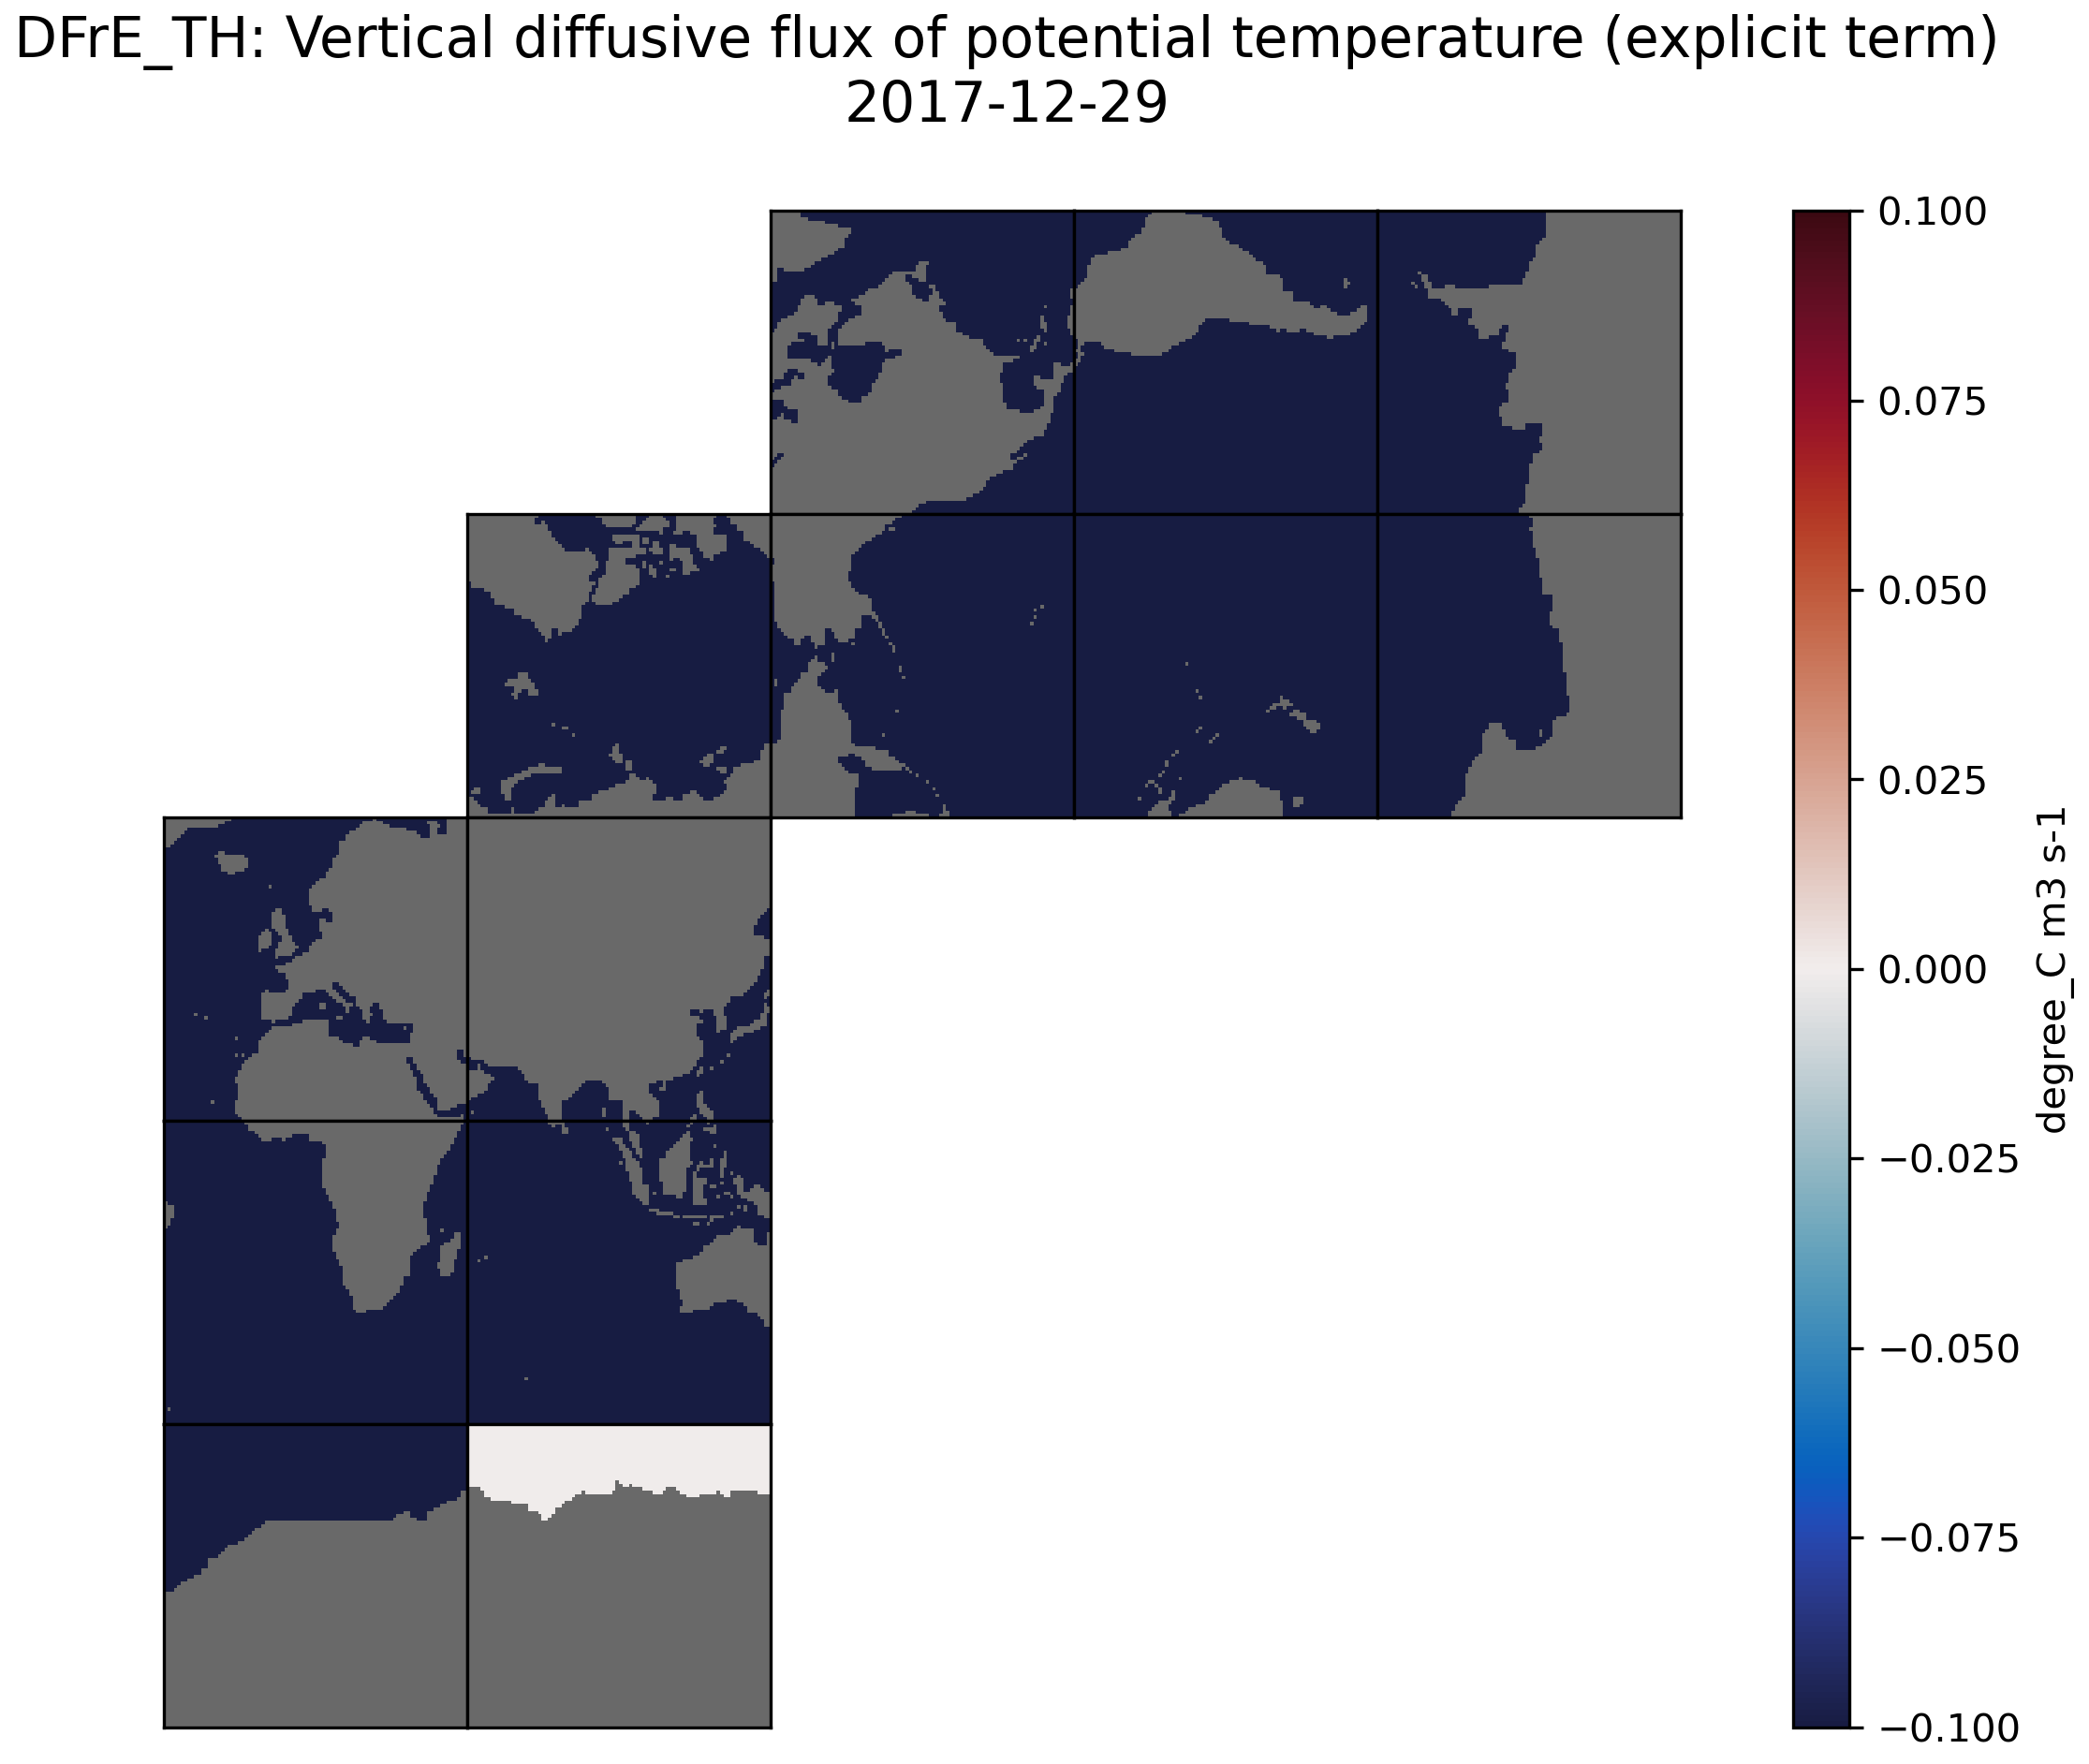
\includegraphics[scale=0.5]{../images/plots/native_plots/Ocean_Three-Dimensional_Potential_Temperature_Fluxes/DFrE_TH.png}
\caption{\\Dataset: OCEAN\_3D\_TEMPERATURE\_FLUX\\Variable: DFrE\_TH}
\label{tab:table-OCEAN_3D_TEMPERATURE_FLUX_DFrE_TH-Plot}
\end{figure}
\pagebreak
\subsubsection{Native Variable DFrI\_TH}
\begin{longtable}{|p{0.06\textwidth}|p{0.41\textwidth}|p{0.39\textwidth}|p{0.06\textwidth}|}
\caption{CDL description of OCEAN\_3D\_TEMPERATURE\_FLUX's DFrI\_TH variable}
\label{tab:table-OCEAN_3D_TEMPERATURE_FLUX_DFrI_TH} \\ 
\hline \endhead \hline \endfoot
\rowcolor{lightgray} \textbf{Storage Type} & \textbf{Variable Name} & \textbf{Description} & \textbf{Unit} \\ \hline
float32 & DFrI\_TH & Vertical diffusive flux of potential temperature (implicit term) & degree\_C m3 s-1 \\ \hline
\rowcolor{lightgray}  \multicolumn{4}{|p{1.00\textwidth}|}{\textbf{CDL Description}} \\ \hline
\multicolumn{4}{|p{1.00\textwidth}|}{\makecell{\parbox{1\textwidth}{float32 DFrI\_TH(time, k\_l, tile, j, i)\\
\hspace*{0.5cm}DFrI\_TH: \_FillValue = 9.96921e+36\\
\hspace*{0.5cm}DFrI\_TH: long\_name = Vertical diffusive flux of potential temperature (implicit term)\\
\hspace*{0.5cm}DFrI\_TH: units = degree\_C m3 s: 1\\
\hspace*{0.5cm}DFrI\_TH: coverage\_content\_type = modelResult\\
\hspace*{0.5cm}DFrI\_TH: direction = >0 decreases potential temperature (THETA)\\
\hspace*{0.5cm}DFrI\_TH: coordinates = XC YC time Zl\\
\hspace*{0.5cm}DFrI\_TH: valid\_min = : 104210688.0\\
\hspace*{0.5cm}DFrI\_TH: valid\_max = 23574302.0}}} \\ \hline
\rowcolor{lightgray} \multicolumn{4}{|p{1.00\textwidth}|}{\textbf{Comments}} \\ \hline
\multicolumn{4}{|p{1\textwidth}|}{The implicit term of the vertical diffusive flux of potential temperature (THETA) in the +z direction through the top 'w' face of the tracer cell on the native model grid. In the ECCO V4r4 model, an implicit scheme is used to calculate vertical diffusive tracer fluxes due to background diffusivity and the Kwz component of the GM-Redi tensor (vertical flux as a function of vertical gradient) while an explicit scheme is used to calculate the vertical diffusive fluxes from the Kwx and Kwy components of the GM-Redi tensor (vertical flux as a function of horizontal gradient). Both implicit and explicit components of vertical diffusive flux of potential temperature are provided. Note: in the Arakawa-C grid, vertical flux quantities are staggered relative to the tracer cells with indexing such that +DFrI\_TH(i,j,k\_l) corresponds to upward +z fluxes through the top 'w' face of the tracer cell at (i,j,k)} \\ \hline
\end{longtable}

\begin{figure}[H]
\centering
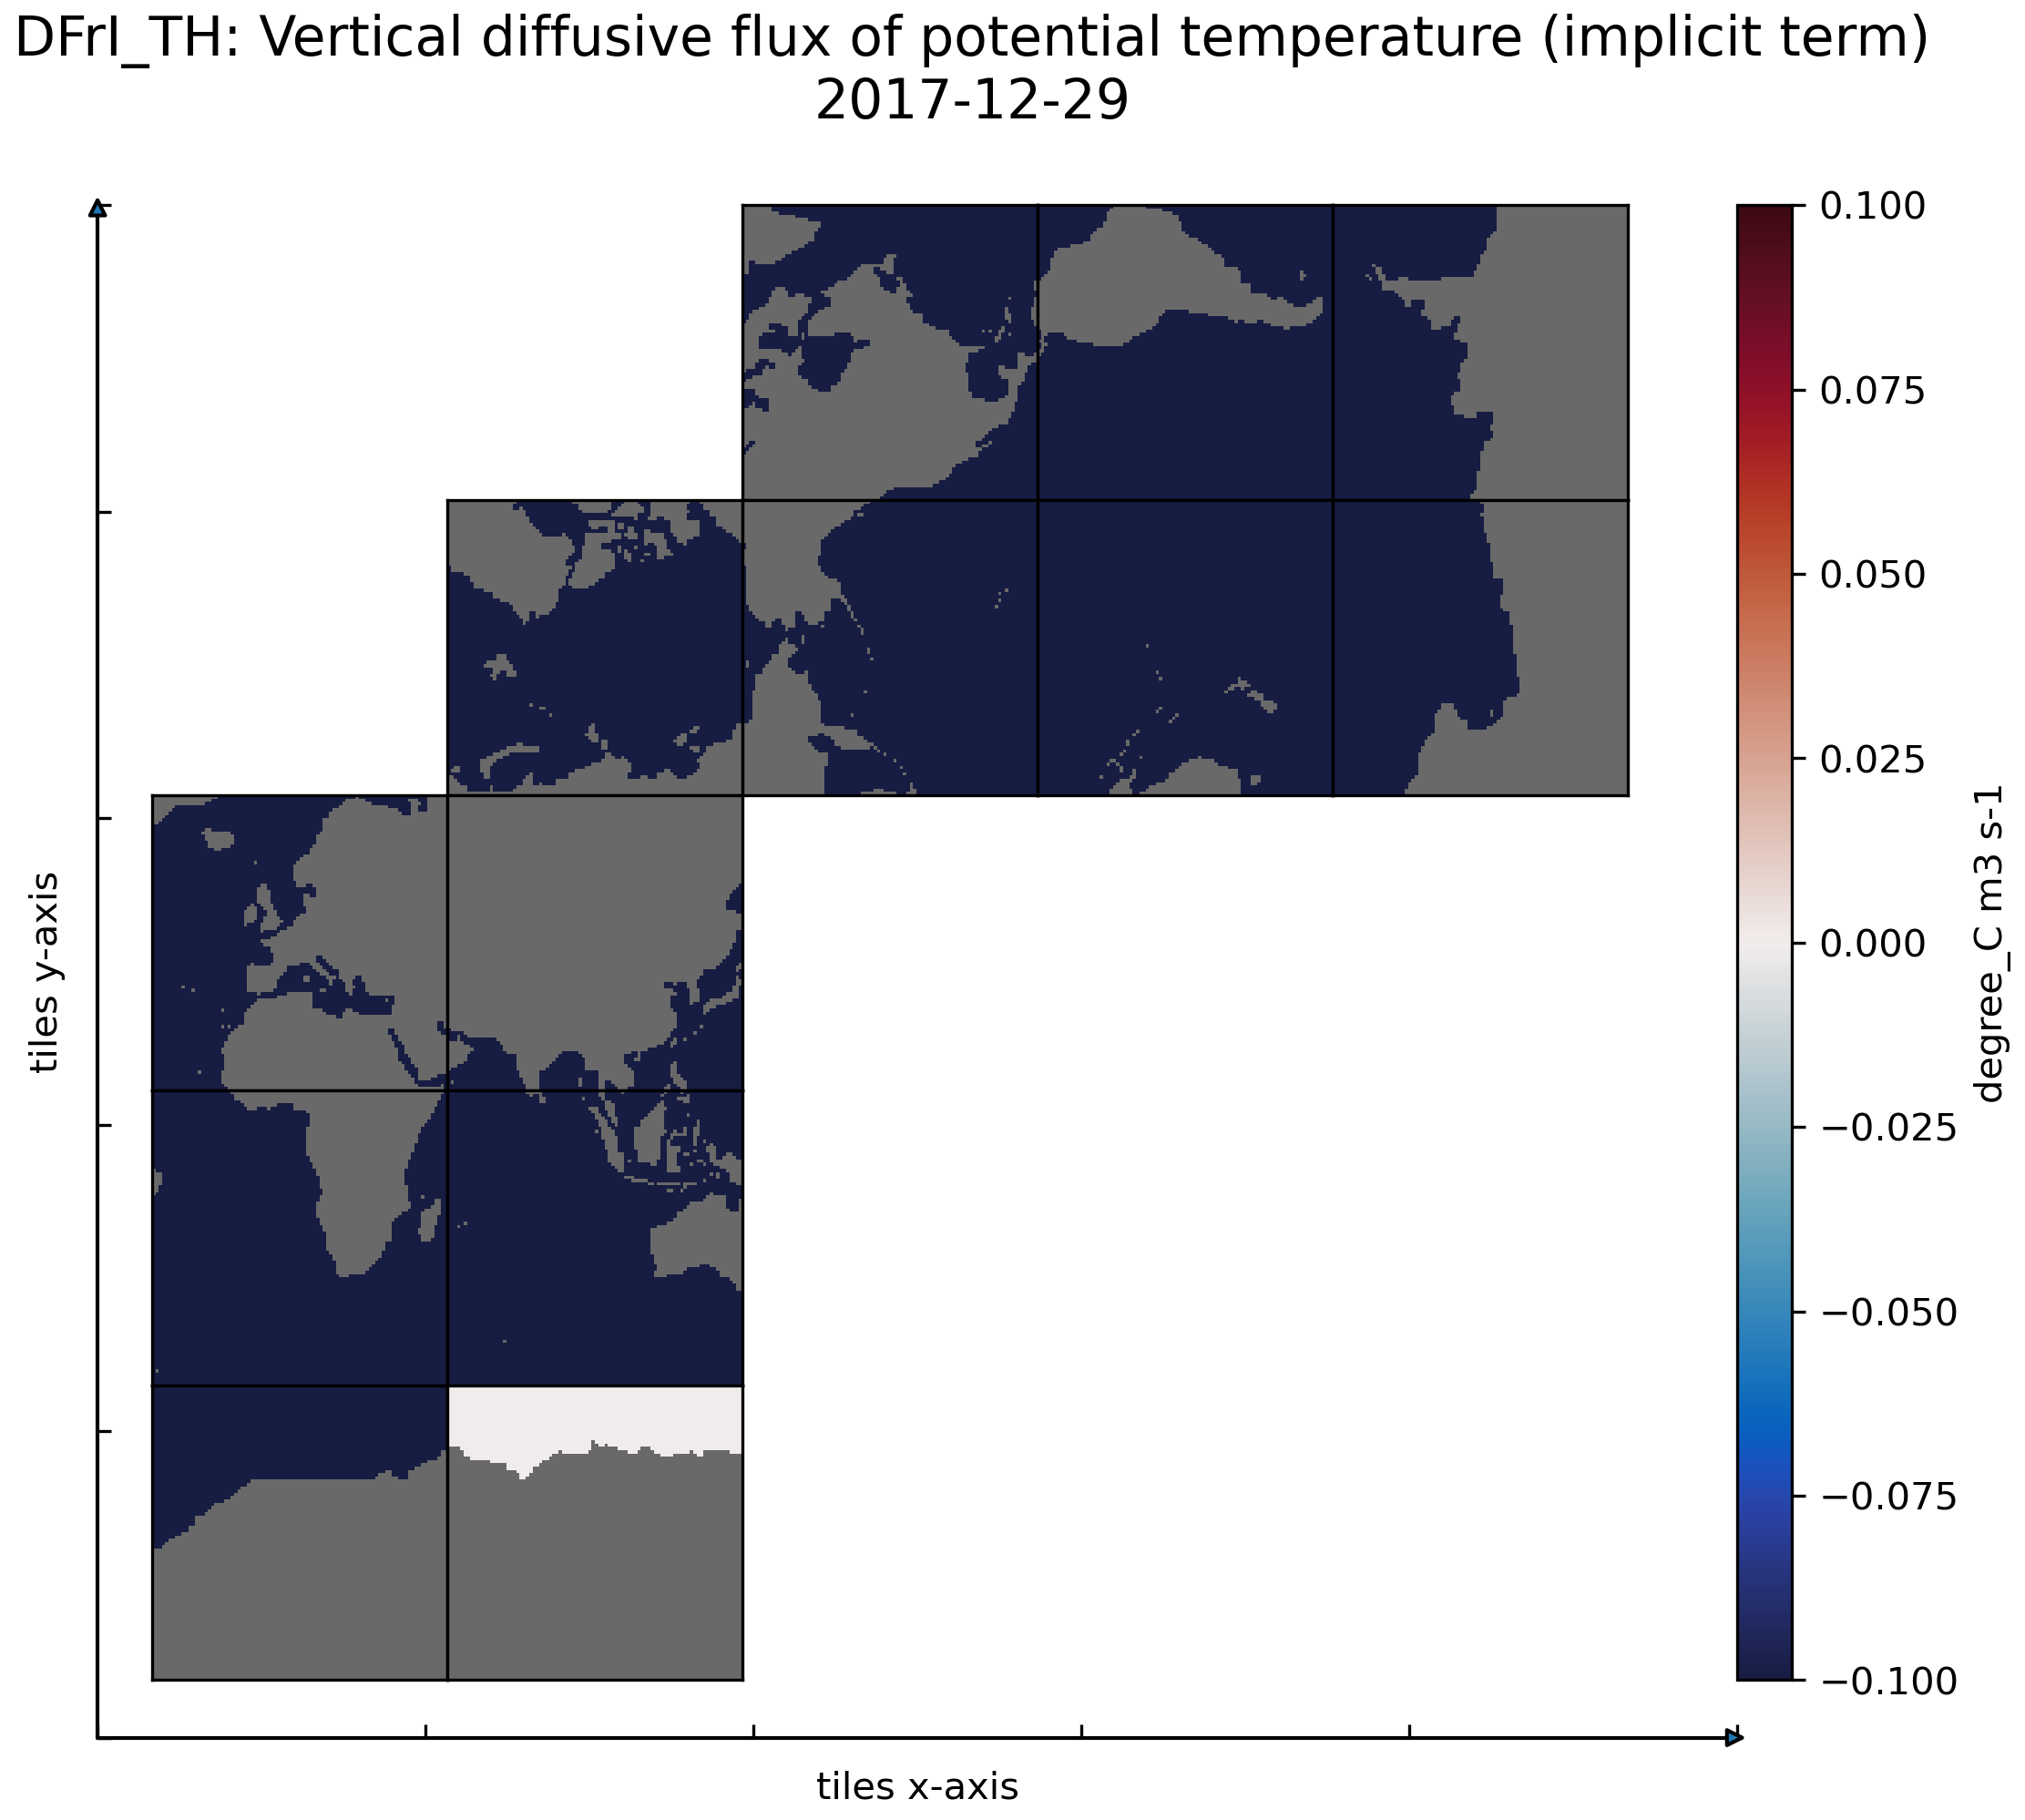
\includegraphics[scale=0.5]{../images/plots/native_plots/Ocean_Three-Dimensional_Potential_Temperature_Fluxes/DFrI_TH.png}
\caption{\\Dataset: OCEAN\_3D\_TEMPERATURE\_FLUX\\Variable: DFrI\_TH}
\label{tab:table-OCEAN_3D_TEMPERATURE_FLUX_DFrI_TH-Plot}
\end{figure}
\pagebreak
\subsubsection{Native Variable DFxE\_TH}
\begin{longtable}{|p{0.06\textwidth}|p{0.41\textwidth}|p{0.39\textwidth}|p{0.06\textwidth}|}
\caption{CDL description of OCEAN\_3D\_TEMPERATURE\_FLUX's DFxE\_TH variable}
\label{tab:table-OCEAN_3D_TEMPERATURE_FLUX_DFxE_TH} \\ 
\hline \endhead \hline \endfoot
\rowcolor{lightgray} \textbf{Storage Type} & \textbf{Variable Name} & \textbf{Description} & \textbf{Unit} \\ \hline
float32 & DFxE\_TH & Lateral diffusive flux of potential temperature in the model +x direction & degree\_C m3 s-1 \\ \hline
\rowcolor{lightgray}  \multicolumn{4}{|p{1.00\textwidth}|}{\textbf{CDL Description}} \\ \hline
\multicolumn{4}{|p{1.00\textwidth}|}{\makecell{\parbox{1\textwidth}{float32 DFxE\_TH(time, k, tile, j, i\_g)\\
\hspace*{0.5cm}DFxE\_TH: \_FillValue = 9.96921e+36\\
\hspace*{0.5cm}DFxE\_TH: long\_name = Lateral diffusive flux of potential temperature in the model +x direction\\
\hspace*{0.5cm}DFxE\_TH: units = degree\_C m3 s: 1\\
\hspace*{0.5cm}DFxE\_TH: mate = DFyE\_TH\\
\hspace*{0.5cm}DFxE\_TH: coverage\_content\_type = modelResult\\
\hspace*{0.5cm}DFxE\_TH: direction = >0 increases potential temperature (THETA)\\
\hspace*{0.5cm}DFxE\_TH: coordinates = time Z\\
\hspace*{0.5cm}DFxE\_TH: valid\_min = : 582494.125\\
\hspace*{0.5cm}DFxE\_TH: valid\_max = 698695.75}}} \\ \hline
\rowcolor{lightgray} \multicolumn{4}{|p{1.00\textwidth}|}{\textbf{Comments}} \\ \hline
\multicolumn{4}{|p{1\textwidth}|}{Lateral diffusive flux of potential temperature (THETA) in the +x direction through the 'u' face of the tracer cell on the native model grid. Note: in the Arakawa-C grid, horizontal flux quantities are staggered relative to the tracer cells with indexing such that +DFxE\_TH(i\_g,j,k) corresponds to +x fluxes through the 'u' face of the tracer cell at (i,j,k). Also, the model +x direction does not necessarily correspond to the geographical east-west direction because the x and y axes of the model's curvilinear lat-lon-cap (llc) grid have arbitrary orientations which vary within and across tiles.} \\ \hline
\end{longtable}

\begin{figure}[H]
\centering
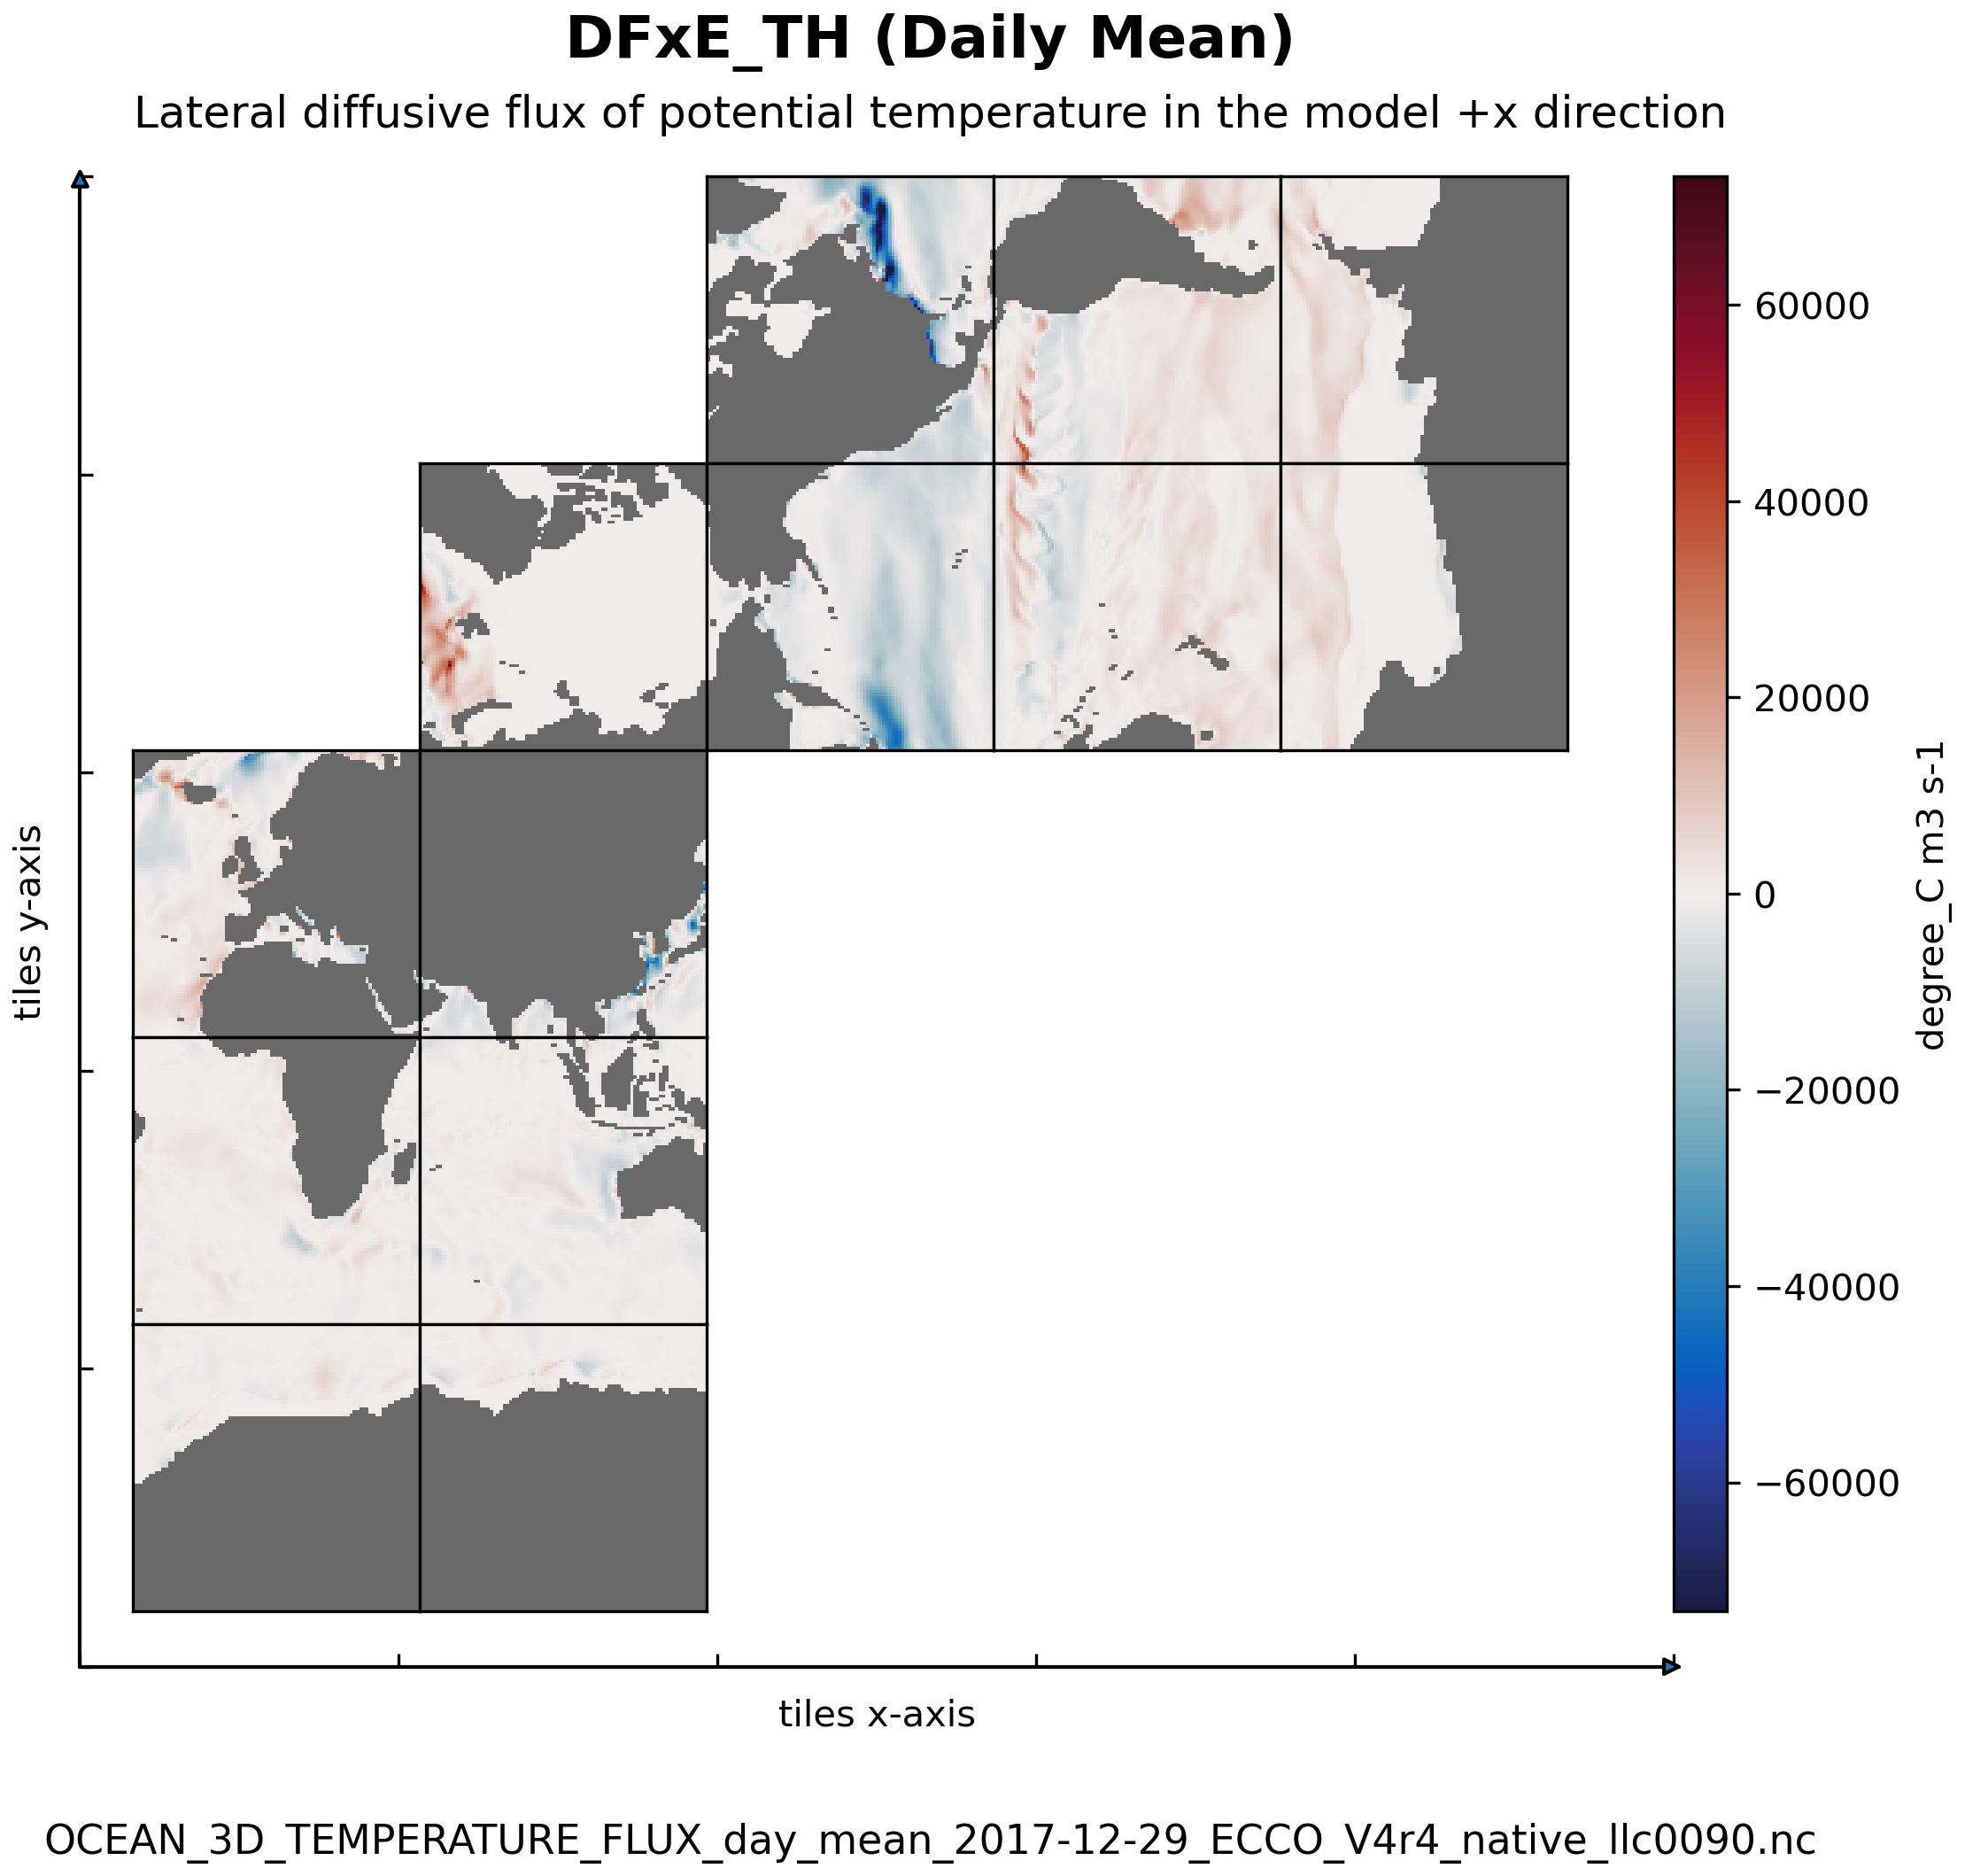
\includegraphics[scale=0.5]{../images/plots/native_plots/Ocean_Three-Dimensional_Potential_Temperature_Fluxes/DFxE_TH.png}
\caption{\\Dataset: OCEAN\_3D\_TEMPERATURE\_FLUX\\Variable: DFxE\_TH}
\label{tab:table-OCEAN_3D_TEMPERATURE_FLUX_DFxE_TH-Plot}
\end{figure}
\pagebreak
\subsubsection{Native Variable DFyE\_TH}
\begin{longtable}{|p{0.06\textwidth}|p{0.41\textwidth}|p{0.39\textwidth}|p{0.06\textwidth}|}
\caption{CDL description of OCEAN\_3D\_TEMPERATURE\_FLUX's DFyE\_TH variable}
\label{tab:table-OCEAN_3D_TEMPERATURE_FLUX_DFyE_TH} \\ 
\hline \endhead \hline \endfoot
\rowcolor{lightgray} \textbf{Storage Type} & \textbf{Variable Name} & \textbf{Description} & \textbf{Unit} \\ \hline
float32 & DFyE\_TH & Lateral diffusive flux of potential temperature in the model +y direction. & degree\_C m3 s-1 \\ \hline
\rowcolor{lightgray}  \multicolumn{4}{|p{1.00\textwidth}|}{\textbf{CDL Description}} \\ \hline
\multicolumn{4}{|p{1.00\textwidth}|}{\makecell{\parbox{1\textwidth}{float32 DFyE\_TH(time, k, tile, j\_g, i)\\
\hspace*{0.5cm}DFyE\_TH: \_FillValue = 9.96921e+36\\
\hspace*{0.5cm}DFyE\_TH: long\_name = Lateral diffusive flux of potential temperature in the model +y direction.\\
\hspace*{0.5cm}DFyE\_TH: units = degree\_C m3 s: 1\\
\hspace*{0.5cm}DFyE\_TH: mate = DFxE\_TH\\
\hspace*{0.5cm}DFyE\_TH: coverage\_content\_type = modelResult\\
\hspace*{0.5cm}DFyE\_TH: direction = >0 increases potential temperature (THETA)\\
\hspace*{0.5cm}DFyE\_TH: coordinates = time Z\\
\hspace*{0.5cm}DFyE\_TH: valid\_min = : 421044.78125\\
\hspace*{0.5cm}DFyE\_TH: valid\_max = 1053781.25}}} \\ \hline
\rowcolor{lightgray} \multicolumn{4}{|p{1.00\textwidth}|}{\textbf{Comments}} \\ \hline
\multicolumn{4}{|p{1\textwidth}|}{Lateral diffusive flux of potential temperature (THETA) in the +y direction through the 'v' face of the tracer cell on the native model grid. Note: in the Arakawa-C grid, horizontal flux quantities are staggered relative to the tracer cells with indexing such that +DFyE\_TH(i,j\_g,k) corresponds to +y fluxes through the 'v' face of the tracer cell at (i,j,k). Also, the model +y direction does not necessarily correspond to the geographical north-south direction because the x and y axes of the model's curvilinear lat-lon-cap (llc) grid have arbitrary orientations which vary within and across tiles.} \\ \hline
\end{longtable}

\begin{figure}[H]
\centering
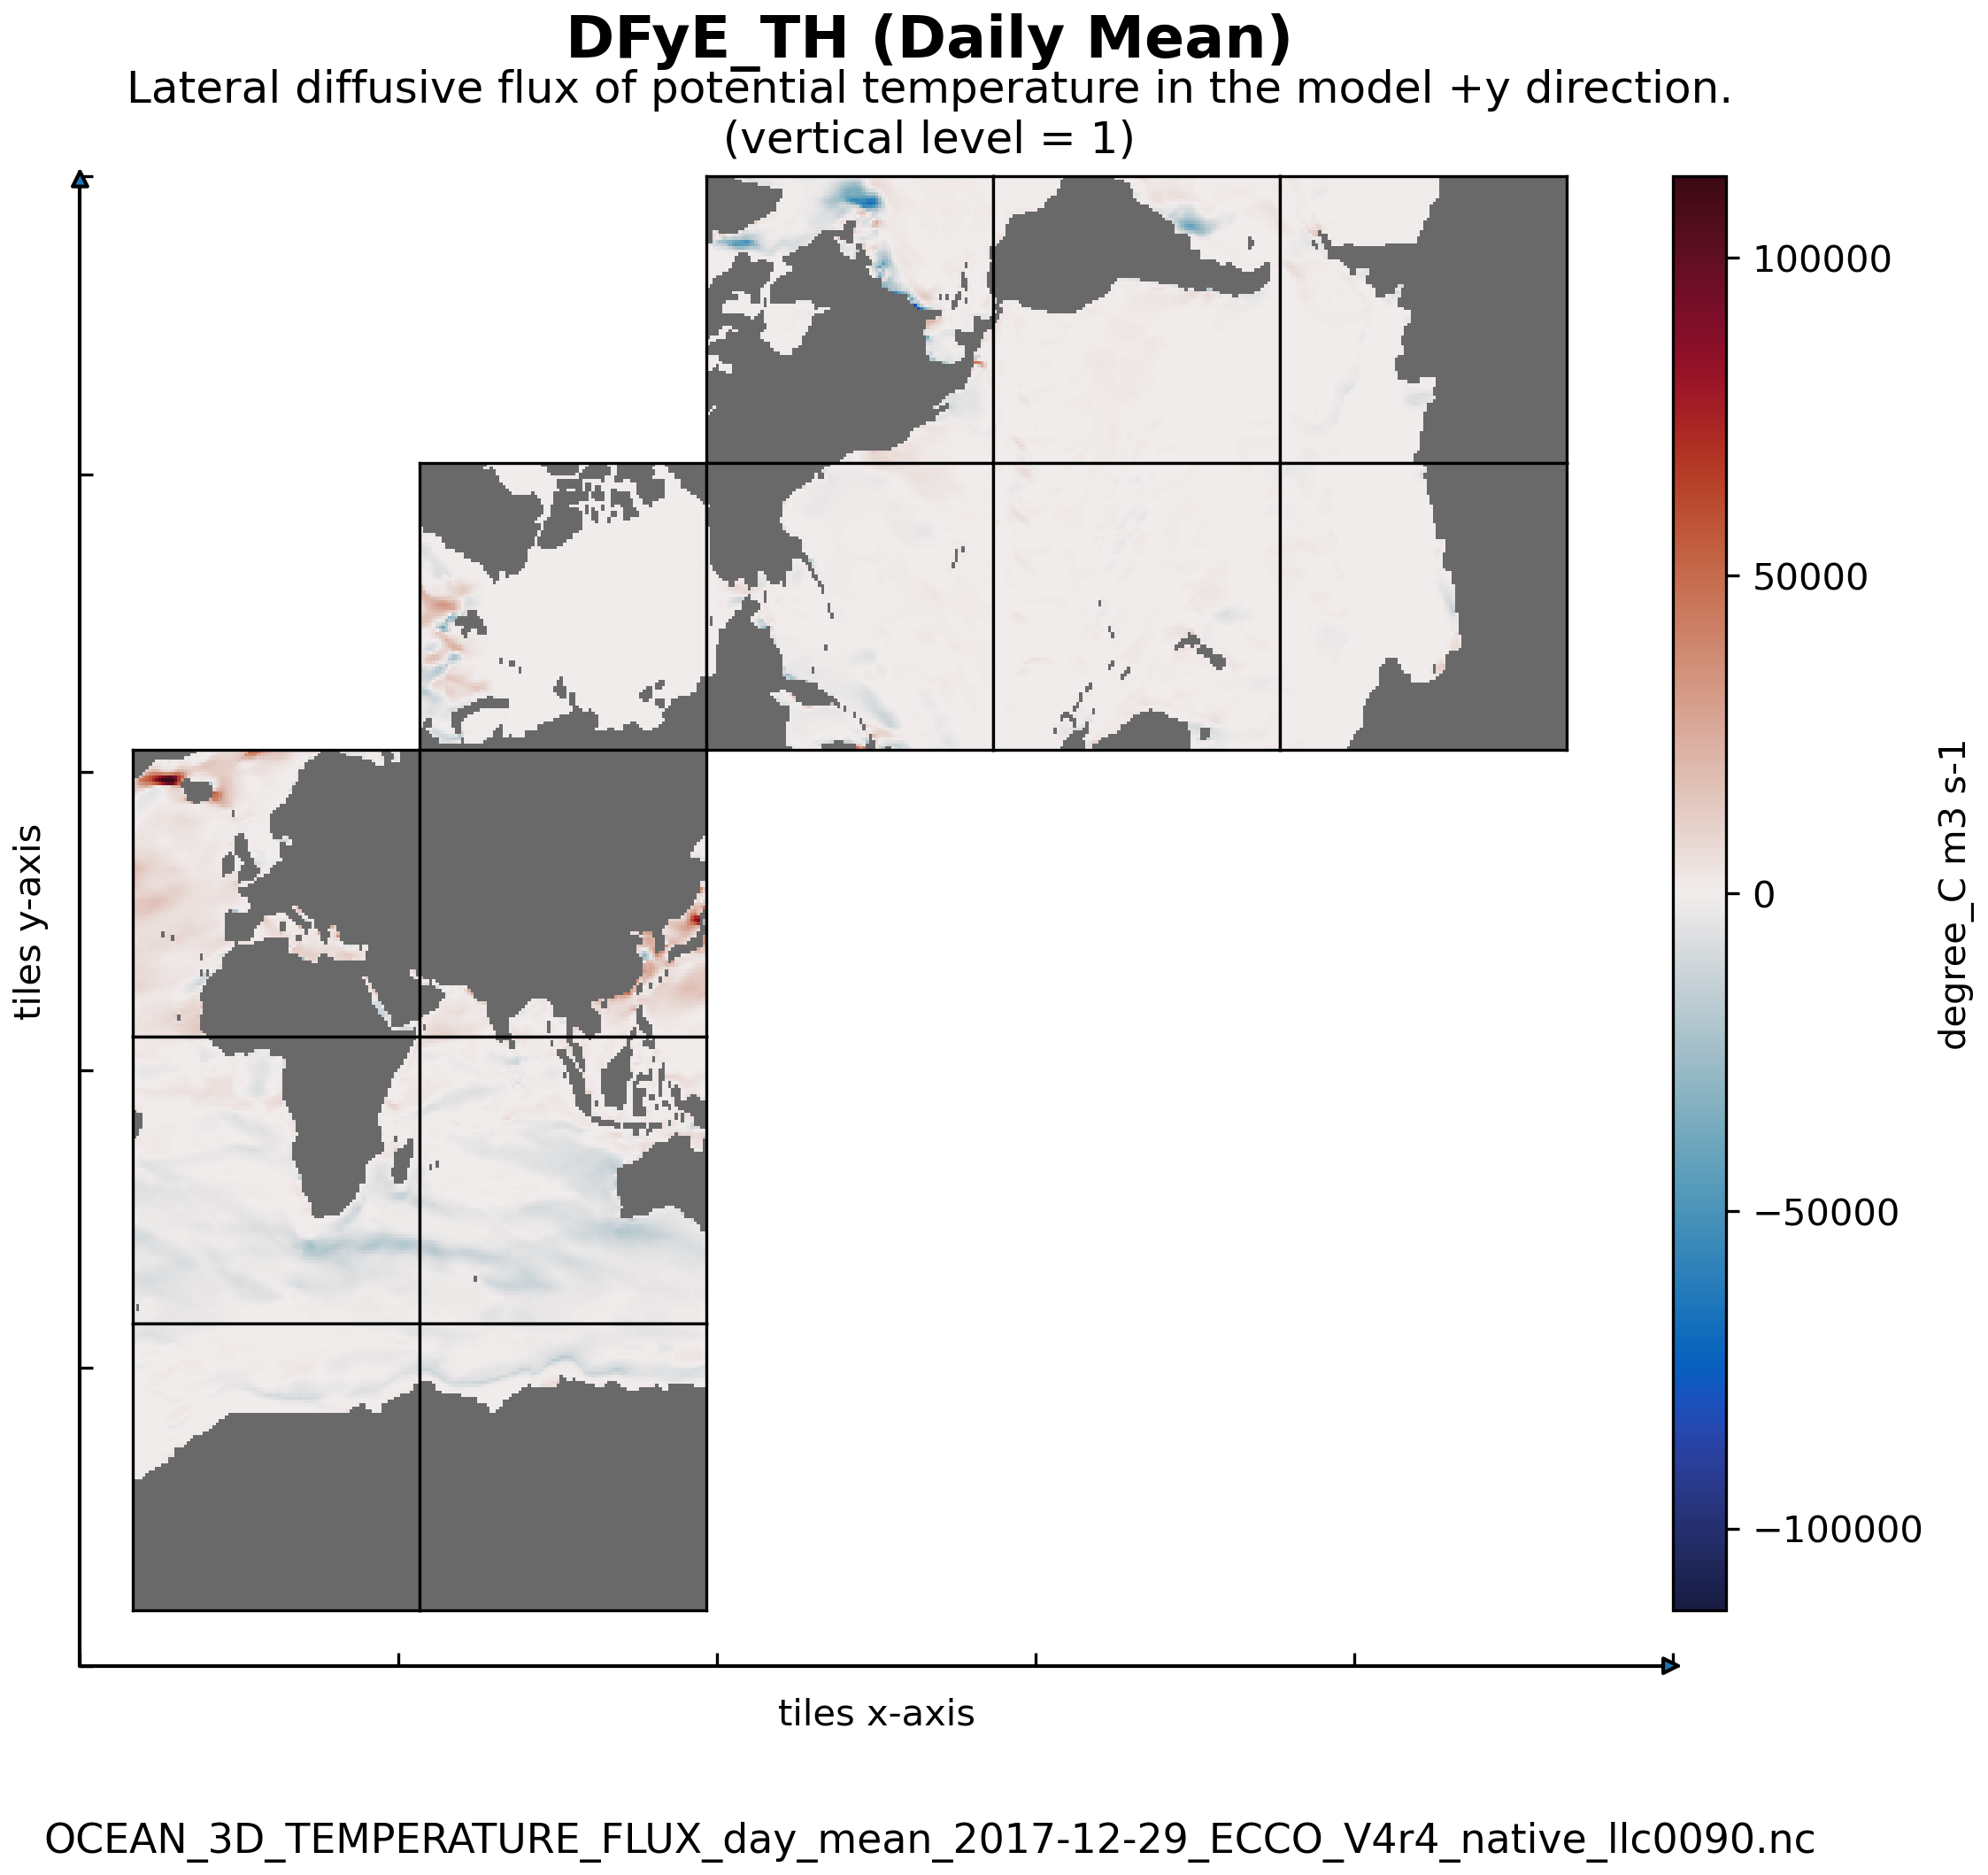
\includegraphics[scale=0.5]{../images/plots/native_plots/Ocean_Three-Dimensional_Potential_Temperature_Fluxes/DFyE_TH.png}
\caption{\\Dataset: OCEAN\_3D\_TEMPERATURE\_FLUX\\Variable: DFyE\_TH}
\label{tab:table-OCEAN_3D_TEMPERATURE_FLUX_DFyE_TH-Plot}
\end{figure}
\pagebreak
\subsection{Native NetCDF OCEAN\_3D\_VOLUME\_FLUX}
\newp
\begin{longtable}{|p{0.1\textwidth}|p{0.5\textwidth}|}
\caption{Variables in the dataset OCEAN\_3D\_VOLUME\_FLUX}
\label{tab:table-OCEAN_3D_VOLUME_FLUX-fields} \\ 
\hline \endhead \hline \endfoot
\rowcolor{lightgray} \textbf{Dataset:} & \textbf{OCEAN\_3D\_VOLUME\_FLUX} \\ \hline
Field: &UVELMASS \\ \hline
Field: &VVELMASS \\ \hline
Field: &WVELMASS \\ \hline
\end{longtable}

\pagebreak
\subsubsection{Native Variable UVELMASS}
\begin{longtable}{|p{0.06\textwidth}|p{0.41\textwidth}|p{0.39\textwidth}|p{0.06\textwidth}|}
\caption{CDL description of OCEAN\_3D\_VOLUME\_FLUX's UVELMASS variable}
\label{tab:table-OCEAN_3D_VOLUME_FLUX_UVELMASS} \\ 
\hline \endhead \hline \endfoot
\rowcolor{lightgray} \textbf{Storage Type} & \textbf{Variable Name} & \textbf{Description} & \textbf{Unit} \\ \hline
float32 & UVELMASS & Horizontal velocity in the model +x direction per unit area of the grid cell 'u' face & m s-1 \\ \hline
\rowcolor{lightgray}  \multicolumn{4}{|p{1.00\textwidth}|}{\textbf{CDL Description}} \\ \hline
\multicolumn{4}{|p{1.00\textwidth}|}{\makecell{\parbox{1\textwidth}{float32 UVELMASS(time, k, tile, j, i\_g)\\
\hspace*{0.5cm}UVELMASS: \_FillValue = 9.96921e+36\\
\hspace*{0.5cm}UVELMASS: long\_name = "Horizontal velocity in the model +x direction per unit area of the grid cell u face"\\
\hspace*{0.5cm}UVELMASS: units = m s: 1\\
\hspace*{0.5cm}UVELMASS: mate = VVELMASS\\
\hspace*{0.5cm}UVELMASS: coverage\_content\_type = modelResult\\
\hspace*{0.5cm}UVELMASS: direction = >0 increases volume\\
\hspace*{0.5cm}UVELMASS: coordinates = Z time\\
\hspace*{0.5cm}UVELMASS: valid\_min = : 2.115365505218506\\
\hspace*{0.5cm}UVELMASS: valid\_max = 2.0377726554870605}}} \\ \hline
\rowcolor{lightgray} \multicolumn{4}{|p{1.00\textwidth}|}{\textbf{Comments}} \\ \hline
\multicolumn{4}{|p{1\textwidth}|}{Horizontal velocity in the model +x direction averaged over the area of the tracer grid cell 'u' face on the native model grid ('u' grid cell face area = drF dyG). Accounts for partial cells (hFacW < 1) and for time-varying grid cell thickness (z* coordinate system). Volume flux in +x = UVELMASS drF dyG. Note: in the Arakawa-C grid, horizontal velocities are staggered relative to the tracer cells with indexing such that +UVELMASS(i,j,k) corresponds to +x fluxes through the 'u' face of the tracer cell at (i,j,k). UVELMASS can be used for volume flux calculations because it accounts for the grid cell thicknesses variations in the +x direction (hFacW) with time (z* coordinate system). Also, the model +x direction does not necessarily correspond to the geographical east-west direction because the x and y axes of the model's curvilinear lat-lon-cap (llc) grid have arbitrary orientations which vary within and across tiles. See VVELMASS and WVELMASS} \\ \hline
\end{longtable}

\begin{figure}[H]
\centering
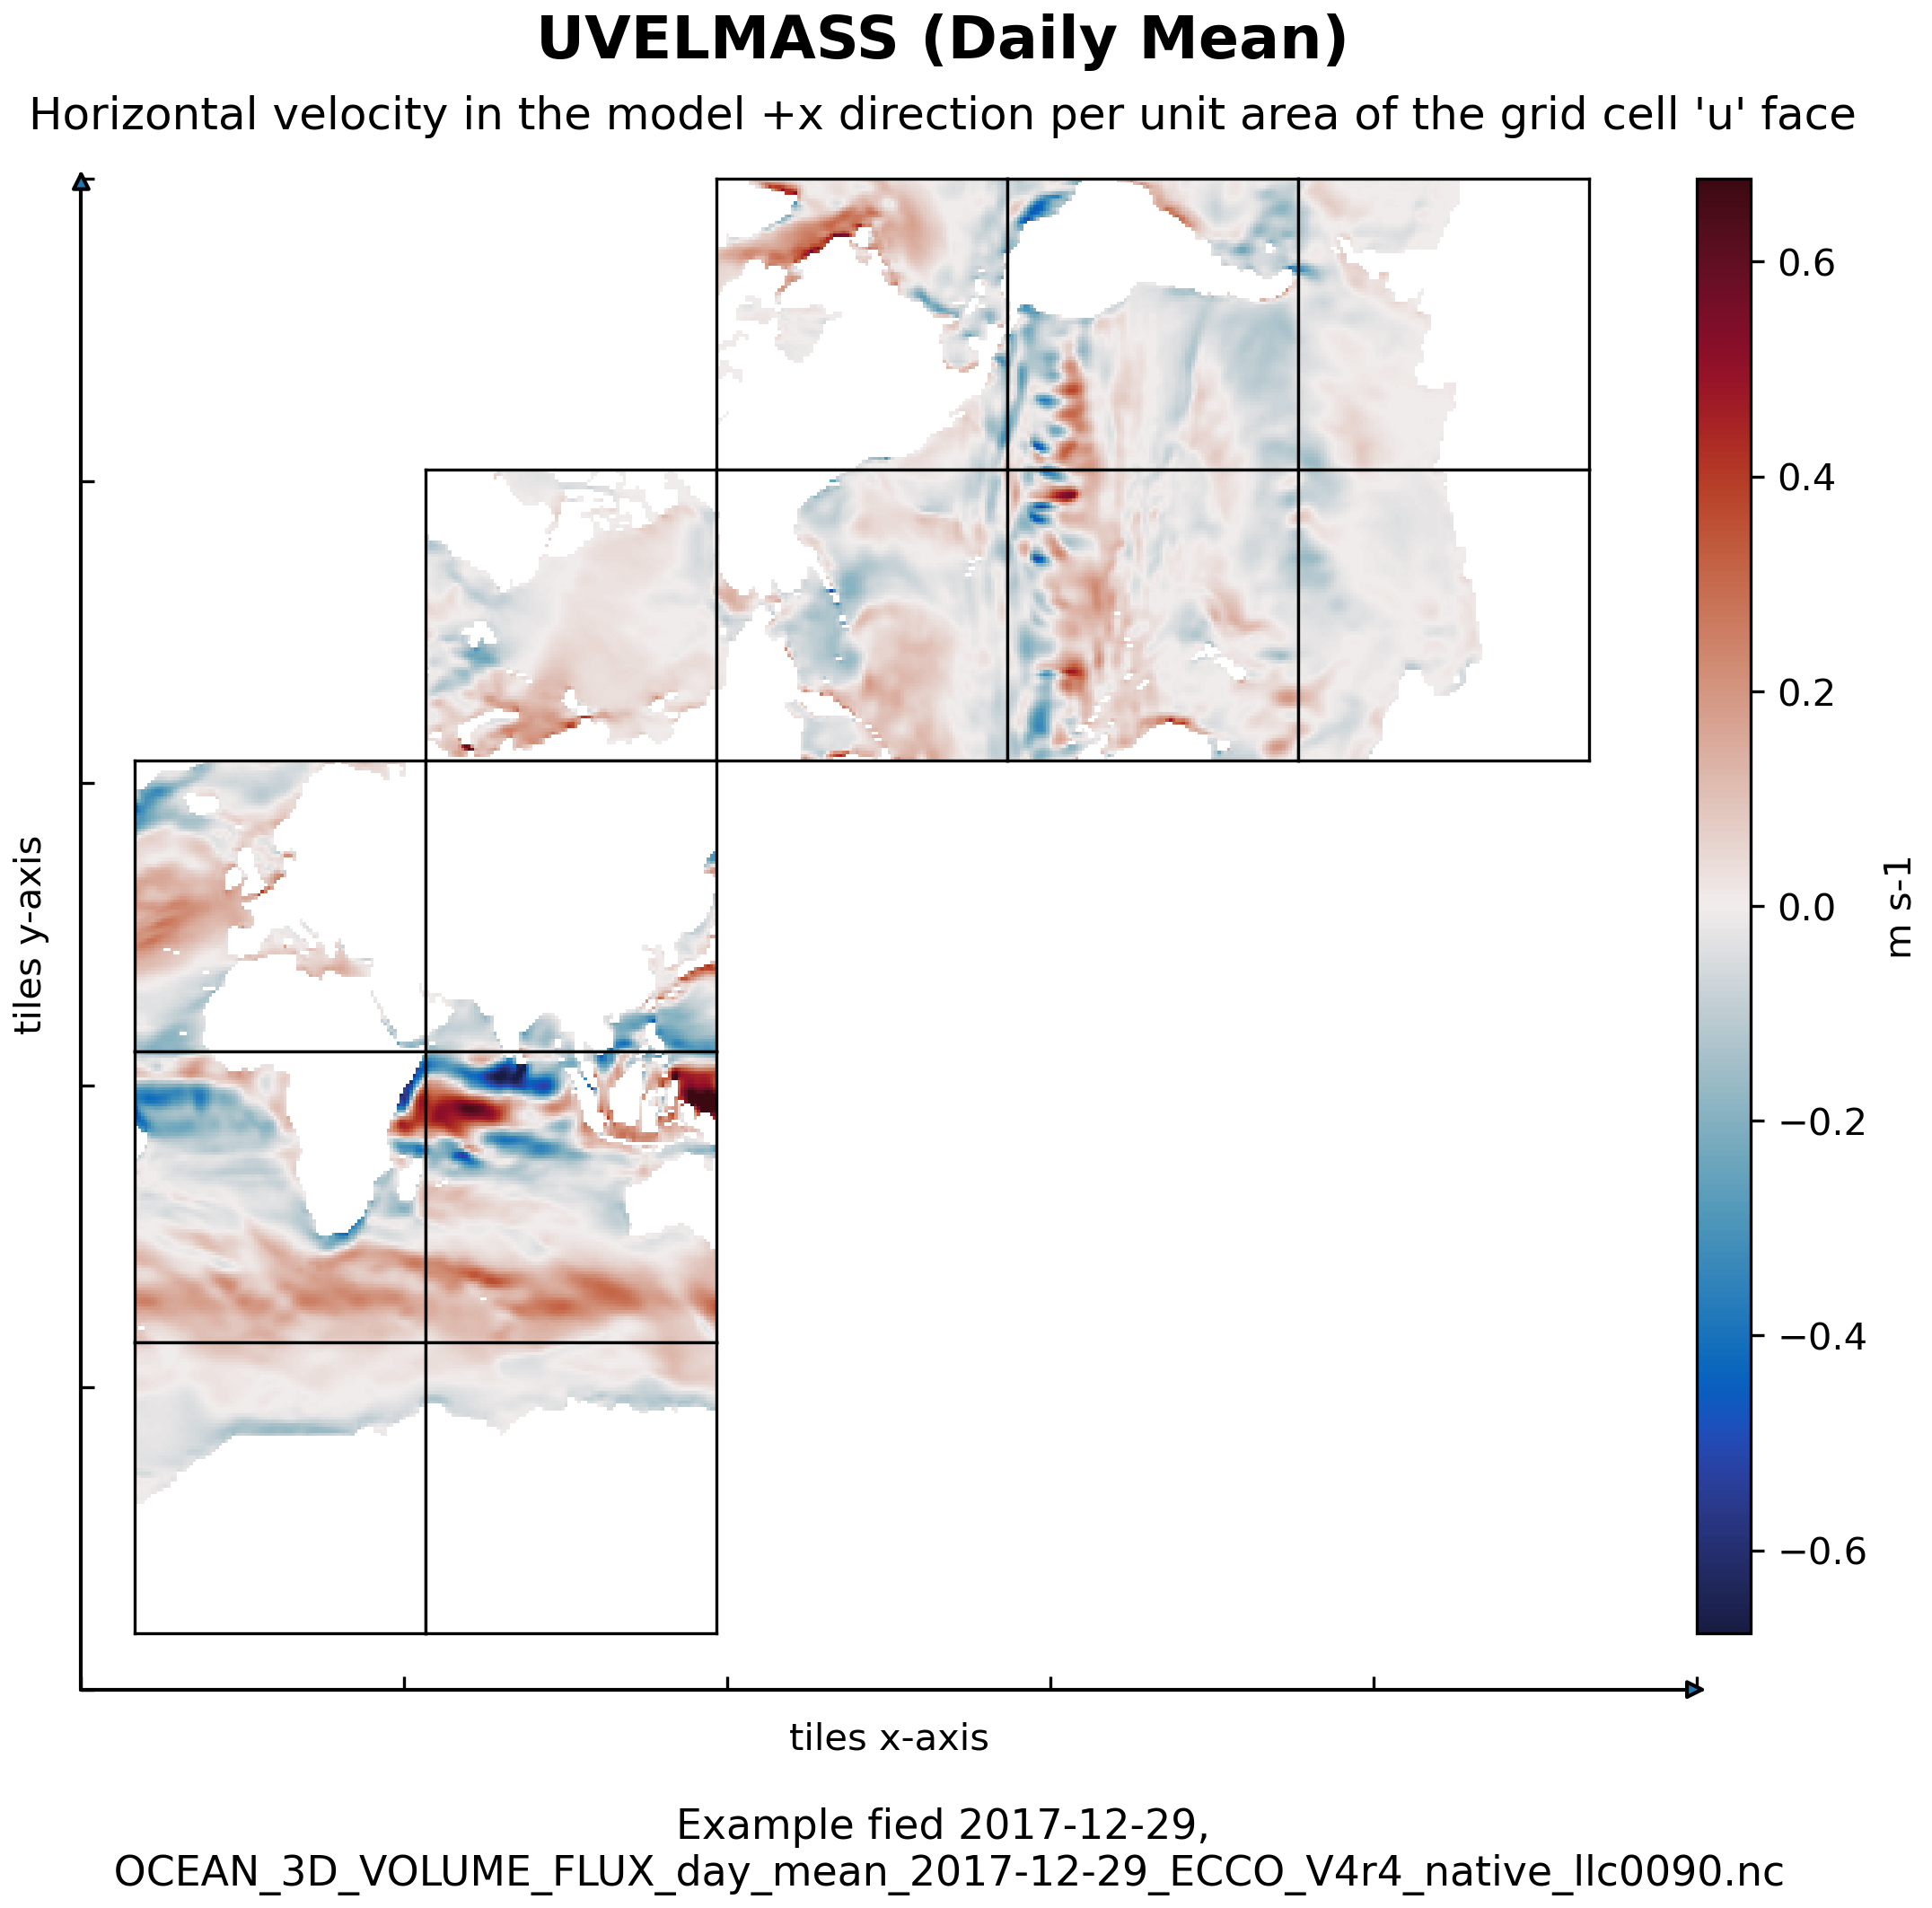
\includegraphics[scale=0.5]{../images/plots/native_plots/Ocean_Three-Dimensional_Volume_Fluxes/UVELMASS.png}
\caption{\\Dataset: OCEAN\_3D\_VOLUME\_FLUX\\Variable: UVELMASS}
\label{tab:table-OCEAN_3D_VOLUME_FLUX_UVELMASS-Plot}
\end{figure}
\pagebreak
\subsubsection{Native Variable VVELMASS}
\begin{longtable}{|p{0.06\textwidth}|p{0.41\textwidth}|p{0.39\textwidth}|p{0.06\textwidth}|}
\caption{CDL description of OCEAN\_3D\_VOLUME\_FLUX's VVELMASS variable}
\label{tab:table-OCEAN_3D_VOLUME_FLUX_VVELMASS} \\ 
\hline \endhead \hline \endfoot
\rowcolor{lightgray} \textbf{Storage Type} & \textbf{Variable Name} & \textbf{Description} & \textbf{Unit} \\ \hline
float32 & VVELMASS & Horizontal velocity in the model +y direction per unit area of the grid cell 'v' face & m s-1 m3 m-3 \\ \hline
\rowcolor{lightgray}  \multicolumn{4}{|p{1.00\textwidth}|}{\textbf{CDL Description}} \\ \hline
\multicolumn{4}{|p{1.00\textwidth}|}{\makecell{\parbox{1\textwidth}{float32 VVELMASS(time, k, tile, j\_g, i)\\
\hspace*{0.5cm}VVELMASS: \_FillValue = 9.96921e+36\\
\hspace*{0.5cm}VVELMASS: long\_name = "Horizontal velocity in the model +y direction per unit area of the grid cell v face"\\
\hspace*{0.5cm}VVELMASS: units = m s: 1 m3 m: 3\\
\hspace*{0.5cm}VVELMASS: mate = UVELMASS\\
\hspace*{0.5cm}VVELMASS: coverage\_content\_type = modelResult\\
\hspace*{0.5cm}VVELMASS: direction = >0 increases volume\\
\hspace*{0.5cm}VVELMASS: coordinates = Z time\\
\hspace*{0.5cm}VVELMASS: valid\_min = : 1.7897182703018188\\
\hspace*{0.5cm}VVELMASS: valid\_max = 1.9216758012771606}}} \\ \hline
\rowcolor{lightgray} \multicolumn{4}{|p{1.00\textwidth}|}{\textbf{Comments}} \\ \hline
\multicolumn{4}{|p{1\textwidth}|}{Horizontal velocity in the model +y direction averaged over the area of the tracer grid cell 'v' face on the native model grid ('v' grid cell face area = drF dxG). Accounts for partial cells (hFacS < 1) and for time-varying grid cell thickness (z* coordinate system). Volume flux in +y = VVELMASS drF dxG. Note: in the Arakawa-C grid, horizontal velocities are staggered relative to the tracer cells with indexing such that +VVELMASS(i,j,k) corresponds to +y fluxes through the 'v' face of the tracer cell at (i,j,k). VVELMASS can be used for volume flux calculations because it accounts for grid cell thicknesses variations in the +y direction (hFacS) with time (z* coordinate system). Also, the model +y direction does not necessarily correspond to the geographical north-south direction because the x and y axes of the model's curvilinear lat-lon-cap (llc) grid have arbitrary orientations which vary within and across tiles. See UVELMASS and WVELMASS.} \\ \hline
\end{longtable}

\begin{figure}[H]
\centering
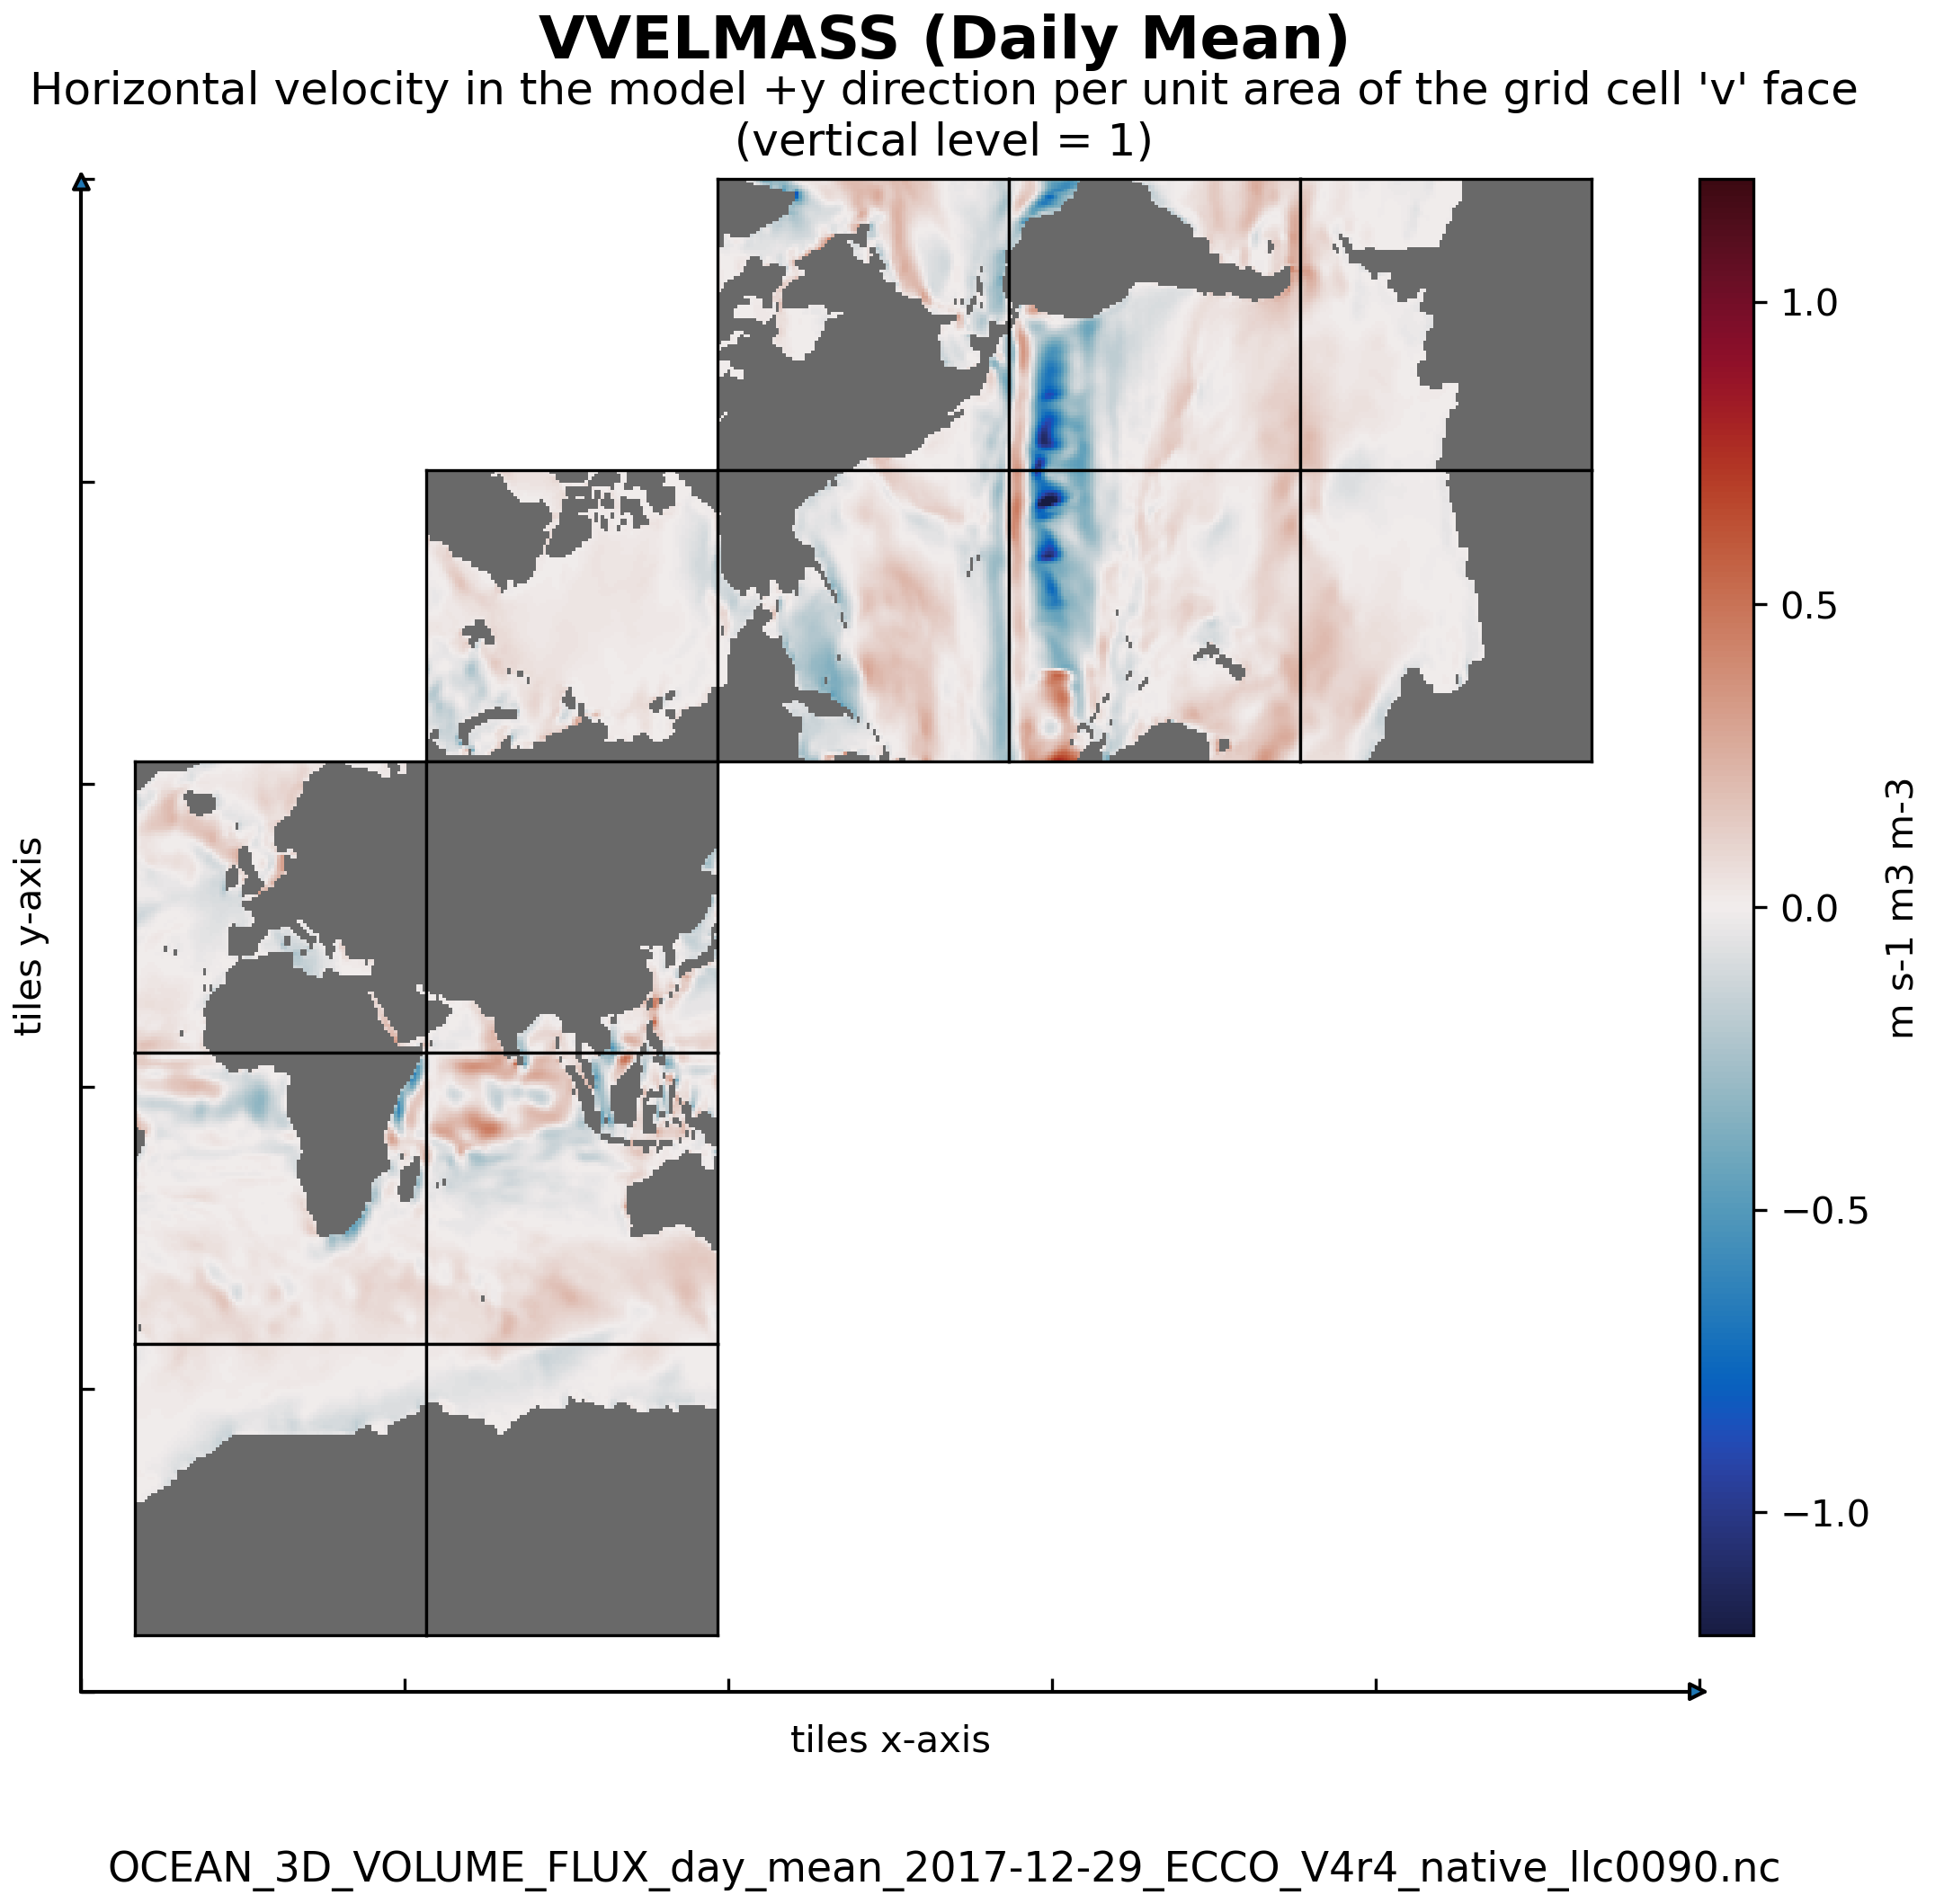
\includegraphics[scale=0.5]{../images/plots/native_plots/Ocean_Three-Dimensional_Volume_Fluxes/VVELMASS.png}
\caption{\\Dataset: OCEAN\_3D\_VOLUME\_FLUX\\Variable: VVELMASS}
\label{tab:table-OCEAN_3D_VOLUME_FLUX_VVELMASS-Plot}
\end{figure}
\pagebreak
\subsubsection{Native Variable WVELMASS}
\begin{longtable}{|p{0.06\textwidth}|p{0.41\textwidth}|p{0.39\textwidth}|p{0.06\textwidth}|}
\caption{CDL description of OCEAN\_3D\_VOLUME\_FLUX's WVELMASS variable}
\label{tab:table-OCEAN_3D_VOLUME_FLUX_WVELMASS} \\ 
\hline \endhead \hline \endfoot
\rowcolor{lightgray} \textbf{Storage Type} & \textbf{Variable Name} & \textbf{Description} & \textbf{Unit} \\ \hline
float32 & WVELMASS & Grid cell face-averaged vertical velocity in the model +z direction. & m s-1 \\ \hline
\rowcolor{lightgray}  \multicolumn{4}{|p{1.00\textwidth}|}{\textbf{CDL Description}} \\ \hline
\multicolumn{4}{|p{1.00\textwidth}|}{\makecell{\parbox{1\textwidth}{float32 WVELMASS(time, k\_l, tile, j, i)\\
\hspace*{0.5cm}WVELMASS: \_FillValue = 9.96921e+36\\
\hspace*{0.5cm}WVELMASS: long\_name = Grid cell face: averaged vertical velocity in the model +z direction.\\
\hspace*{0.5cm}WVELMASS: units = m s: 1\\
\hspace*{0.5cm}WVELMASS: coverage\_content\_type = modelResult\\
\hspace*{0.5cm}WVELMASS: direction = >0 decreases volume\\
\hspace*{0.5cm}WVELMASS: standard\_name = upward\_sea\_water\_velocity\\
\hspace*{0.5cm}WVELMASS: coordinates = YC Zl time XC\\
\hspace*{0.5cm}WVELMASS: valid\_min = : 0.0023150660563260317\\
\hspace*{0.5cm}WVELMASS: valid\_max = 0.0016380994347855449}}} \\ \hline
\rowcolor{lightgray} \multicolumn{4}{|p{1.00\textwidth}|}{\textbf{Comments}} \\ \hline
\multicolumn{4}{|p{1\textwidth}|}{Vertical velocity in the +z direction at the top 'w' face of the tracer cell on the native model grid. Volume flux in +z = WVELMASS drA. Note: in the Arakawa-C grid, vertical velocities are staggered relative to the tracer cells with indexing such that +WVELMASS(i,j,k) corresponds to upward +z motion through the top 'w' face of the tracer cell at (i,j,k). Unlike UVELMASS and VVELMASS, WVELMASS is not scaled by a time-varying open water fraction because the open water fraction of the 'w' face is always 1, thus WVELMASS is identical to WVEL.} \\ \hline
\end{longtable}

\begin{figure}[H]
\centering
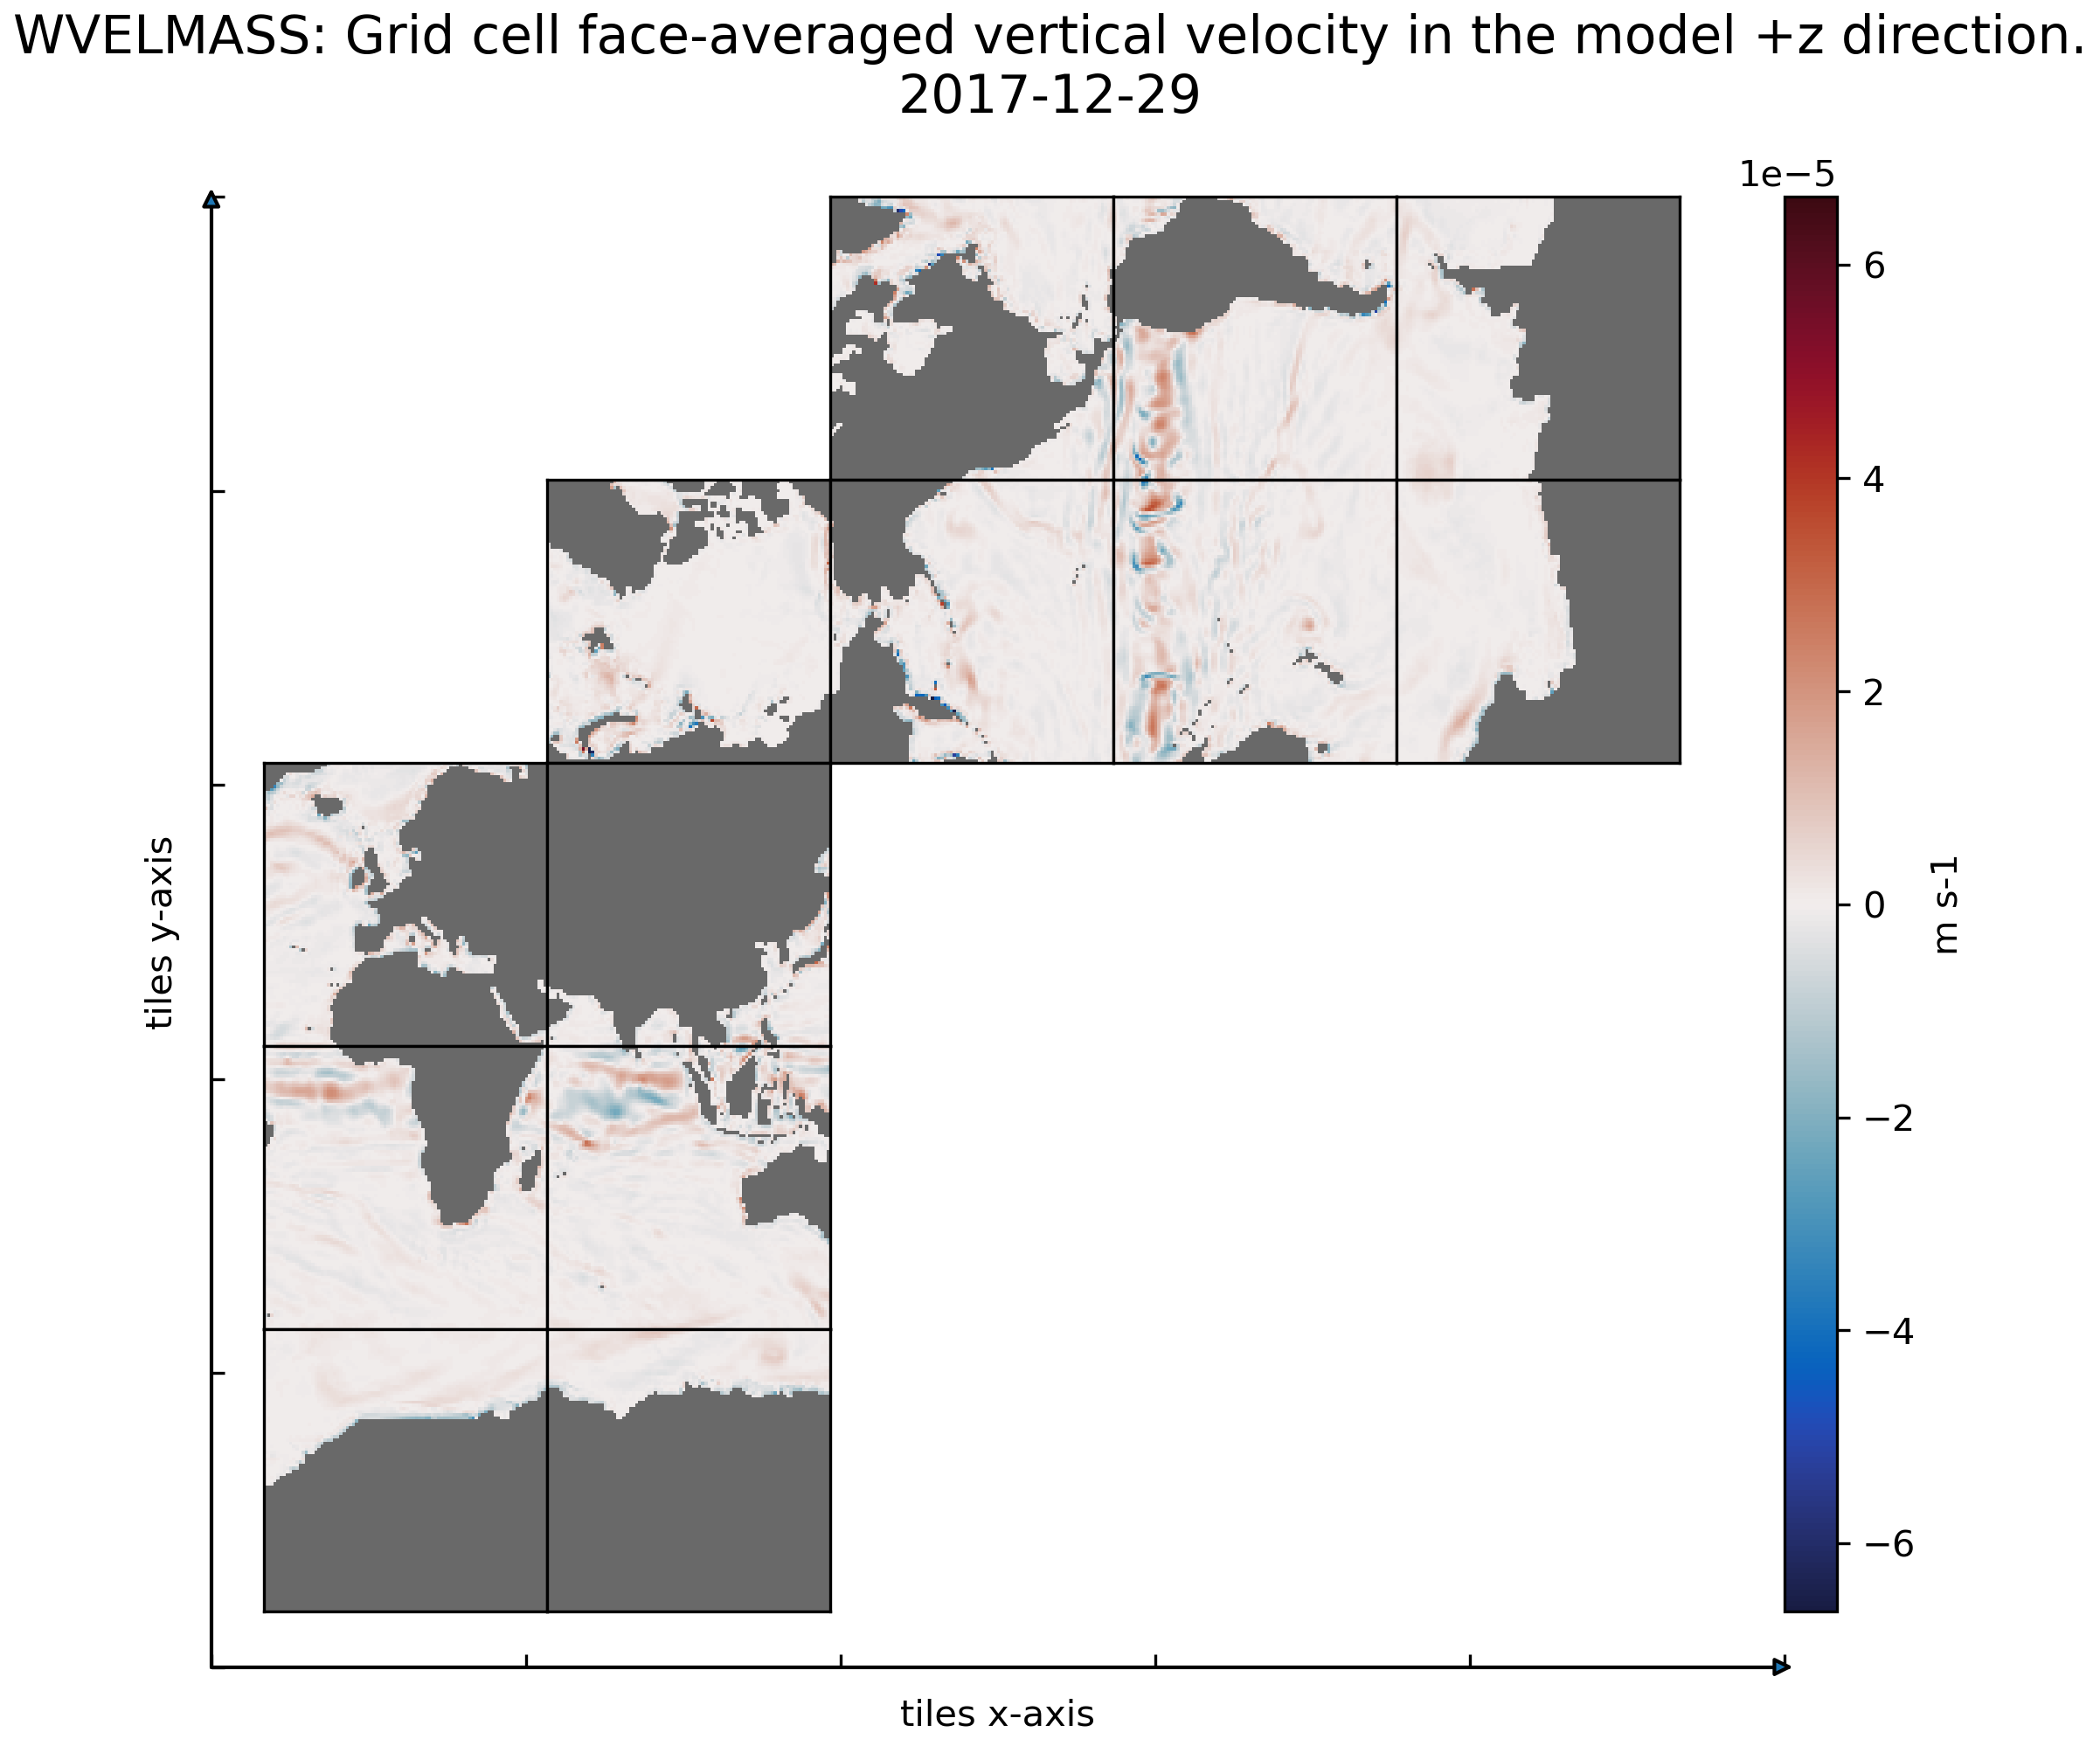
\includegraphics[scale=0.5]{../images/plots/native_plots/Ocean_Three-Dimensional_Volume_Fluxes/WVELMASS.png}
\caption{\\Dataset: OCEAN\_3D\_VOLUME\_FLUX\\Variable: WVELMASS}
\label{tab:table-OCEAN_3D_VOLUME_FLUX_WVELMASS-Plot}
\end{figure}
\pagebreak
\subsection{Native NetCDF OCEAN\_AND\_ICE\_SURFACE\_FW\_FLUX}
\newp
\begin{longtable}{|p{0.1\textwidth}|p{0.5\textwidth}|}
\caption{Variables in the dataset OCEAN\_AND\_ICE\_SURFACE\_FW\_FLUX}
\label{tab:table-OCEAN_AND_ICE_SURFACE_FW_FLUX-fields} \\ 
\hline \endhead \hline \endfoot
\rowcolor{lightgray} \textbf{Dataset:} & \textbf{OCEAN\_AND\_ICE\_SURFACE\_FW\_FLUX} \\ \hline
Field: &EXFpreci \\ \hline
Field: &EXFevap \\ \hline
Field: &EXFroff \\ \hline
Field: &SIsnPrcp \\ \hline
Field: &EXFempmr \\ \hline
Field: &oceFWflx \\ \hline
Field: &SIatmFW \\ \hline
Field: &SFLUX \\ \hline
Field: &SIacSubl \\ \hline
Field: &SIrsSubl \\ \hline
Field: &SIfwThru \\ \hline
\end{longtable}

\pagebreak
\subsubsection{Native Variable EXFempmr}
\begin{longtable}{|p{0.06\textwidth}|p{0.41\textwidth}|p{0.39\textwidth}|p{0.06\textwidth}|}
\caption{CDL description of OCEAN\_AND\_ICE\_SURFACE\_FW\_FLUX's EXFempmr variable}
\label{tab:table-OCEAN_AND_ICE_SURFACE_FW_FLUX_EXFempmr} \\ 
\hline \endhead \hline \endfoot
\rowcolor{lightgray} \textbf{Storage Type} & \textbf{Variable Name} & \textbf{Description} & \textbf{Unit} \\ \hline
float32 & EXFempmr & Open ocean net surface freshwater flux from precipitation, evaporation, and runoff & m s-1 \\ \hline
\rowcolor{lightgray}  \multicolumn{4}{|p{1.00\textwidth}|}{\textbf{CDL Description}} \\ \hline
\multicolumn{4}{|p{1.00\textwidth}|}{\makecell{\parbox{1\textwidth}{float32 EXFempmr(time, tile, j, i)\\
\hspace*{0.5cm}EXFempmr: \_FillValue = 9.96921e+36\\
\hspace*{0.5cm}EXFempmr: long\_name = Open ocean net surface freshwater flux from precipitation\\
evaporation\\
and runoff\\
\hspace*{0.5cm}EXFempmr: units = m s: 1\\
\hspace*{0.5cm}EXFempmr: coverage\_content\_type = modelResult\\
\hspace*{0.5cm}EXFempmr: direction = >0 increases salinity (SALT)\\
\hspace*{0.5cm}EXFempmr: coordinates = YC XC time\\
\hspace*{0.5cm}EXFempmr: valid\_min = : 8.299433829961345e: 06\\
\hspace*{0.5cm}EXFempmr: valid\_max = 5.400421514423215e: 07}}} \\ \hline
\rowcolor{lightgray} \multicolumn{4}{|p{1.00\textwidth}|}{\textbf{Comments}} \\ \hline
\multicolumn{4}{|p{1\textwidth}|}{Net surface freshwater flux from precipitation, evaporation, and runoff per unit area in open water (not covered by sea-ice). Excludes freshwater fluxes involving sea-ice and snow. Note: calculated as EXFevap-EXFpreci-EXFroff.} \\ \hline
\end{longtable}

\begin{figure}[H]
\centering
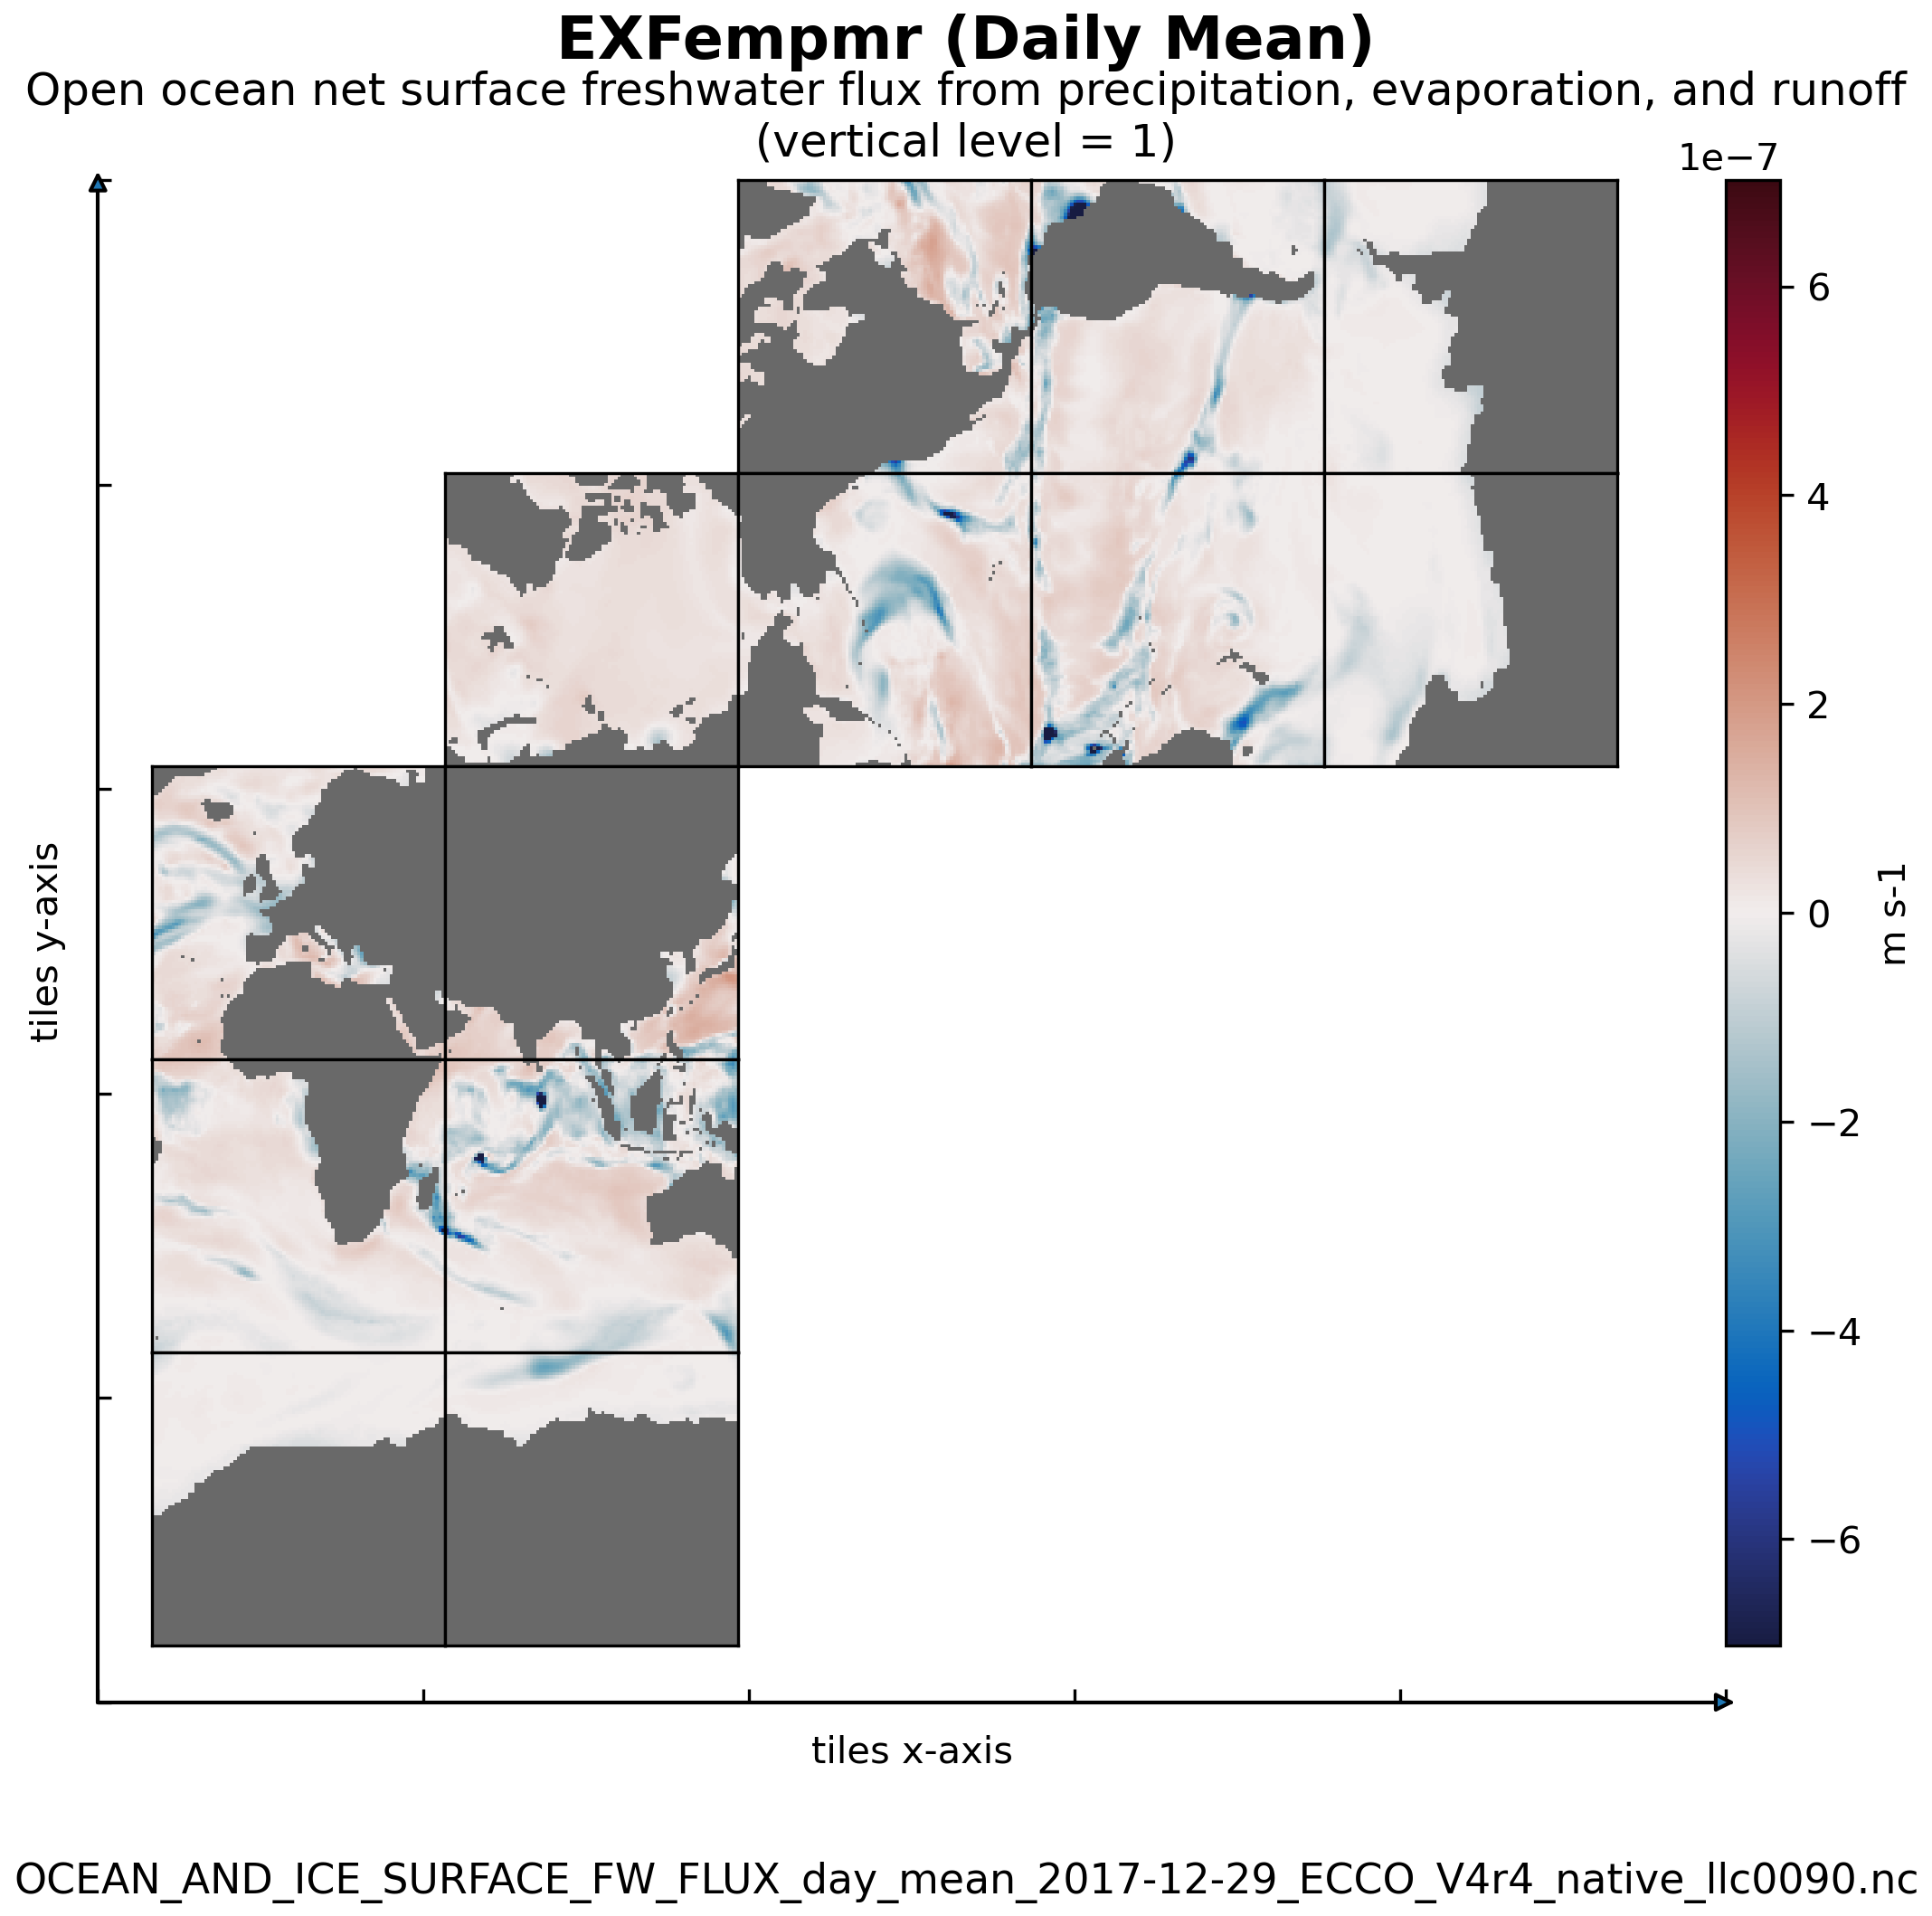
\includegraphics[scale=0.5]{../images/plots/native_plots/Ocean_and_Sea-Ice_Surface_Freshwater_Fluxes/EXFempmr.png}
\caption{\\Dataset: OCEAN\_AND\_ICE\_SURFACE\_FW\_FLUX\\Variable: EXFempmr}
\label{tab:table-OCEAN_AND_ICE_SURFACE_FW_FLUX_EXFempmr-Plot}
\end{figure}
\pagebreak
\subsubsection{Native Variable EXFevap}
\begin{longtable}{|p{0.06\textwidth}|p{0.41\textwidth}|p{0.39\textwidth}|p{0.06\textwidth}|}
\caption{CDL description of OCEAN\_AND\_ICE\_SURFACE\_FW\_FLUX's EXFevap variable}
\label{tab:table-OCEAN_AND_ICE_SURFACE_FW_FLUX_EXFevap} \\ 
\hline \endhead \hline \endfoot
\rowcolor{lightgray} \textbf{Storage Type} & \textbf{Variable Name} & \textbf{Description} & \textbf{Unit} \\ \hline
float32 & EXFevap & Open ocean evaporation rate & m s-1 \\ \hline
\rowcolor{lightgray}  \multicolumn{4}{|p{1.00\textwidth}|}{\textbf{CDL Description}} \\ \hline
\multicolumn{4}{|p{1.00\textwidth}|}{\makecell{\parbox{1\textwidth}{float32 EXFevap(time, tile, j, i)\\
\hspace*{0.5cm}EXFevap: \_FillValue = 9.96921e+36\\
\hspace*{0.5cm}EXFevap: long\_name = Open ocean evaporation rate\\
\hspace*{0.5cm}EXFevap: units = m s: 1\\
\hspace*{0.5cm}EXFevap: coverage\_content\_type = modelResult\\
\hspace*{0.5cm}EXFevap: direction = >0 increases salinity (SALT)\\
\hspace*{0.5cm}EXFevap: standard\_name = lwe\_water\_evaporation\_rate\\
\hspace*{0.5cm}EXFevap: coordinates = YC XC time\\
\hspace*{0.5cm}EXFevap: valid\_min = : 1.0958113705328287e: 07\\
\hspace*{0.5cm}EXFevap: valid\_max = 7.090054623404285e: 07}}} \\ \hline
\rowcolor{lightgray} \multicolumn{4}{|p{1.00\textwidth}|}{\textbf{Comments}} \\ \hline
\multicolumn{4}{|p{1\textwidth}|}{Evaporation rate per unit area of open water (not covered by sea-ice). Note: calculated using the bulk formula following Large and Yeager (2004) NCAR/TN-460+STR.} \\ \hline
\end{longtable}

\begin{figure}[H]
\centering
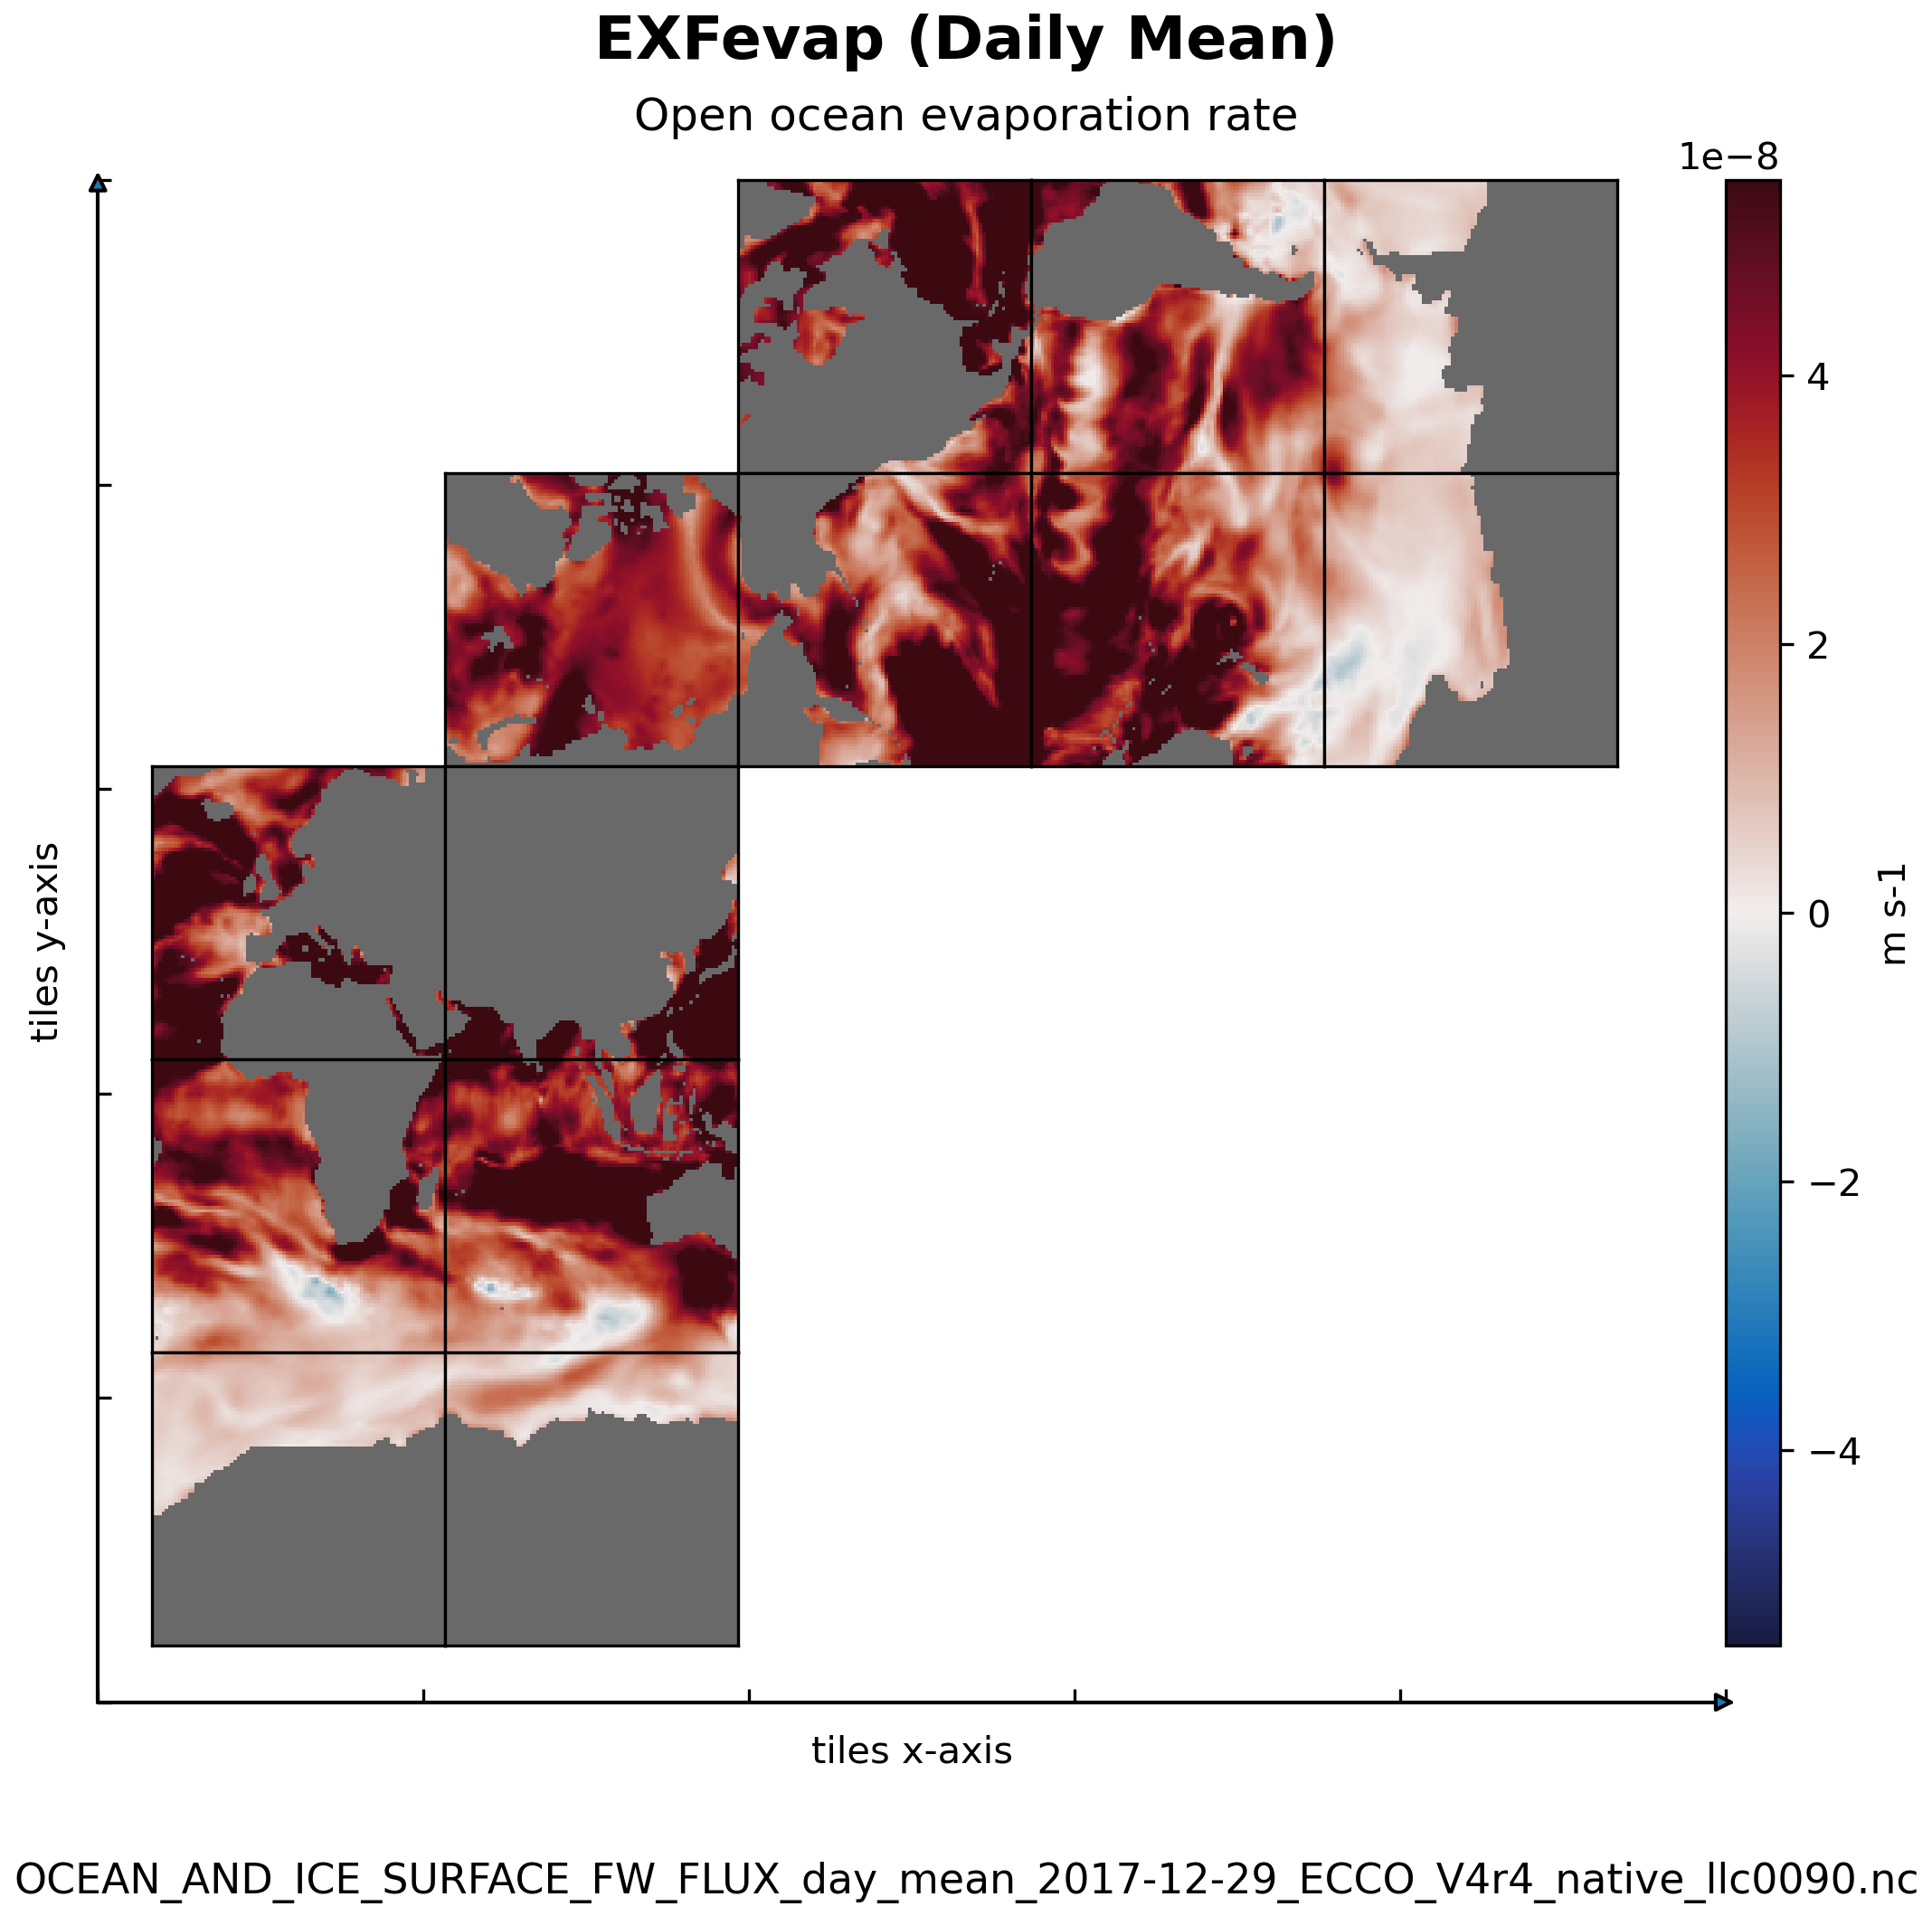
\includegraphics[scale=0.5]{../images/plots/native_plots/Ocean_and_Sea-Ice_Surface_Freshwater_Fluxes/EXFevap.png}
\caption{\\Dataset: OCEAN\_AND\_ICE\_SURFACE\_FW\_FLUX\\Variable: EXFevap}
\label{tab:table-OCEAN_AND_ICE_SURFACE_FW_FLUX_EXFevap-Plot}
\end{figure}
\pagebreak
\subsubsection{Native Variable EXFpreci}
\begin{longtable}{|p{0.06\textwidth}|p{0.41\textwidth}|p{0.39\textwidth}|p{0.06\textwidth}|}
\caption{CDL description of OCEAN\_AND\_ICE\_SURFACE\_FW\_FLUX's EXFpreci variable}
\label{tab:table-OCEAN_AND_ICE_SURFACE_FW_FLUX_EXFpreci} \\ 
\hline \endhead \hline \endfoot
\rowcolor{lightgray} \textbf{Storage Type} & \textbf{Variable Name} & \textbf{Description} & \textbf{Unit} \\ \hline
float32 & EXFpreci & Precipitation rate & m s-1 \\ \hline
\rowcolor{lightgray}  \multicolumn{4}{|p{1.00\textwidth}|}{\textbf{CDL Description}} \\ \hline
\multicolumn{4}{|p{1.00\textwidth}|}{\makecell{\parbox{1\textwidth}{float32 EXFpreci(time, tile, j, i)\\
\hspace*{0.5cm}EXFpreci: \_FillValue = 9.96921e+36\\
\hspace*{0.5cm}EXFpreci: long\_name = Precipitation rate\\
\hspace*{0.5cm}EXFpreci: units = m s: 1\\
\hspace*{0.5cm}EXFpreci: coverage\_content\_type = modelResult\\
\hspace*{0.5cm}EXFpreci: direction = >0 increases salinity (SALT)\\
\hspace*{0.5cm}EXFpreci: standard\_name = lwe\_precipitation\_rate\\
\hspace*{0.5cm}EXFpreci: coordinates = YC XC time\\
\hspace*{0.5cm}EXFpreci: valid\_min = : 1.4860395936011628e: 07\\
\hspace*{0.5cm}EXFpreci: valid\_max = 8.317776519106701e: 06}}} \\ \hline
\rowcolor{lightgray} \multicolumn{4}{|p{1.00\textwidth}|}{\textbf{Comments}} \\ \hline
\multicolumn{4}{|p{1\textwidth}|}{Precipitation rate. Note: sum of ERA-Interim precipitation and the control adjustment from ocean state estimation.} \\ \hline
\end{longtable}

\begin{figure}[H]
\centering
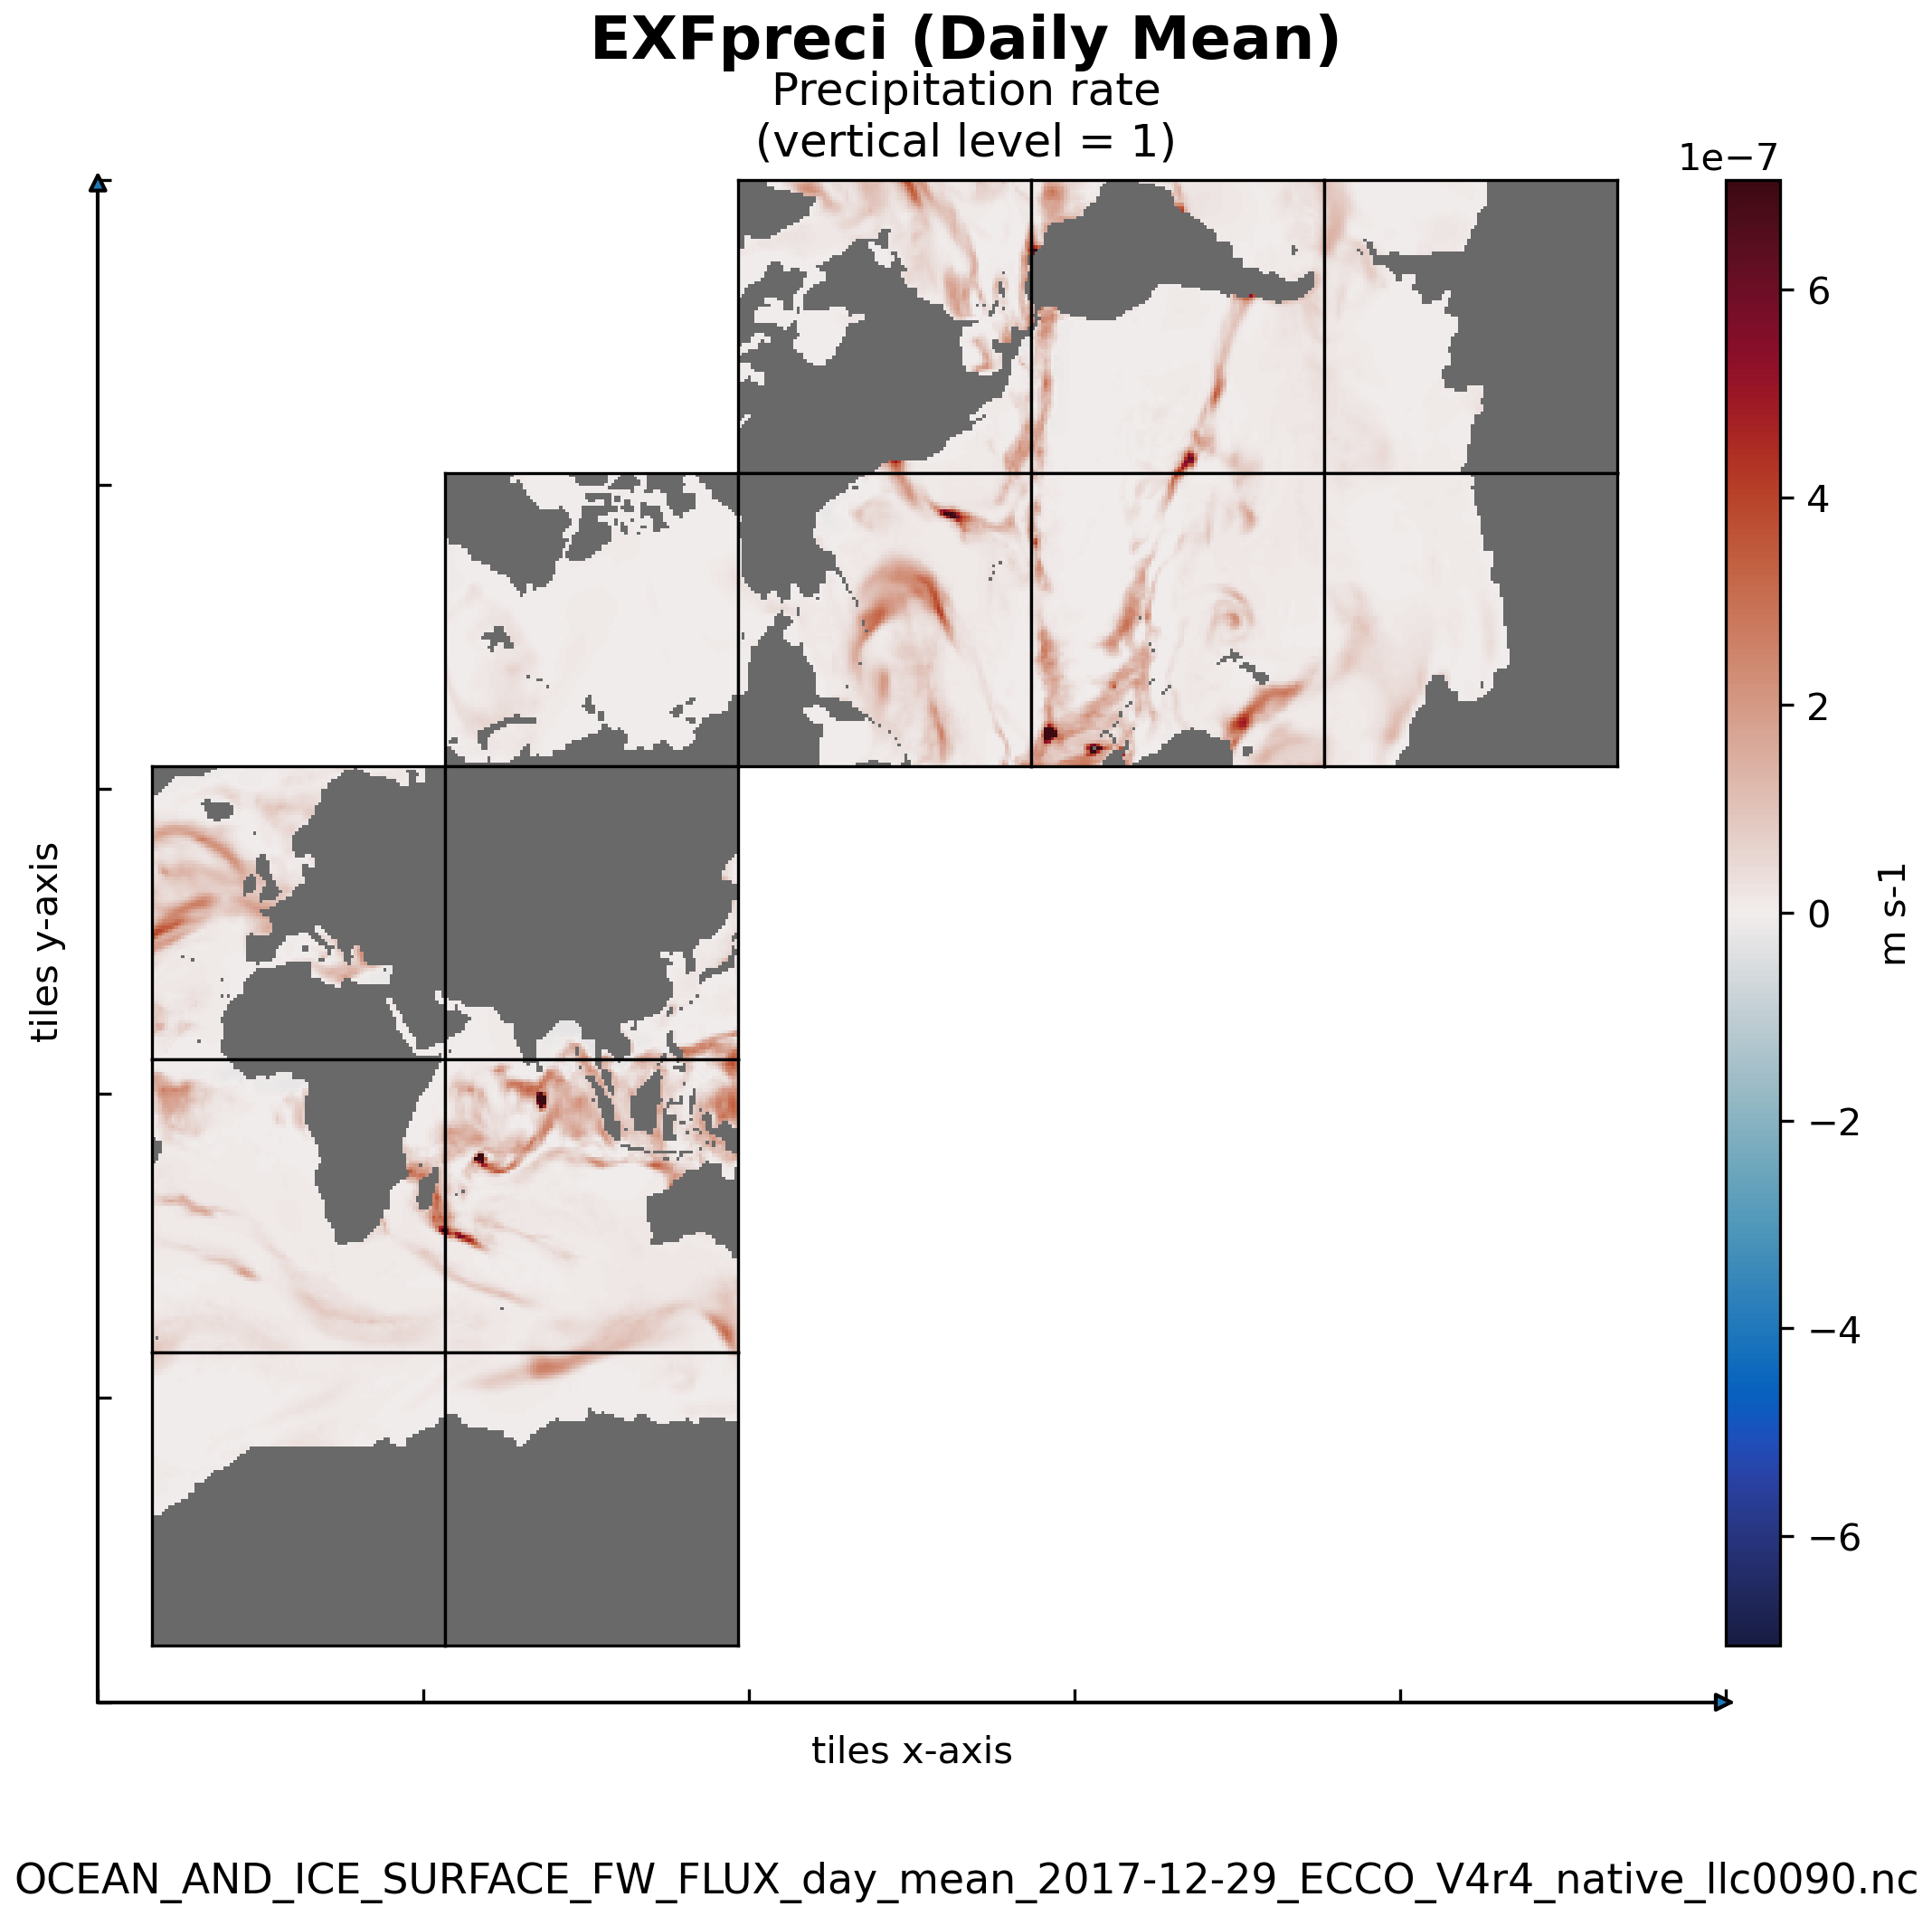
\includegraphics[scale=0.5]{../images/plots/native_plots/Ocean_and_Sea-Ice_Surface_Freshwater_Fluxes/EXFpreci.png}
\caption{\\Dataset: OCEAN\_AND\_ICE\_SURFACE\_FW\_FLUX\\Variable: EXFpreci}
\label{tab:table-OCEAN_AND_ICE_SURFACE_FW_FLUX_EXFpreci-Plot}
\end{figure}
\pagebreak
\subsubsection{Native Variable EXFroff}
\begin{longtable}{|p{0.06\textwidth}|p{0.41\textwidth}|p{0.39\textwidth}|p{0.06\textwidth}|}
\caption{CDL description of OCEAN\_AND\_ICE\_SURFACE\_FW\_FLUX's EXFroff variable}
\label{tab:table-OCEAN_AND_ICE_SURFACE_FW_FLUX_EXFroff} \\ 
\hline \endhead \hline \endfoot
\rowcolor{lightgray} \textbf{Storage Type} & \textbf{Variable Name} & \textbf{Description} & \textbf{Unit} \\ \hline
float32 & EXFroff & River runoff & m s-1 \\ \hline
\rowcolor{lightgray}  \multicolumn{4}{|p{1.00\textwidth}|}{\textbf{CDL Description}} \\ \hline
\multicolumn{4}{|p{1.00\textwidth}|}{\makecell{\parbox{1\textwidth}{float32 EXFroff(time, tile, j, i)\\
\hspace*{0.5cm}EXFroff: \_FillValue = 9.96921e+36\\
\hspace*{0.5cm}EXFroff: long\_name = River runoff\\
\hspace*{0.5cm}EXFroff: units = m s: 1\\
\hspace*{0.5cm}EXFroff: coverage\_content\_type = modelResult\\
\hspace*{0.5cm}EXFroff: direction = >0 increases salinity (SALT)\\
\hspace*{0.5cm}EXFroff: standard\_name = surface\_runoff\_flux\\
\hspace*{0.5cm}EXFroff: coordinates = YC XC time\\
\hspace*{0.5cm}EXFroff: valid\_min = 0.0\\
\hspace*{0.5cm}EXFroff: valid\_max = 4.185612397122895e: 06}}} \\ \hline
\rowcolor{lightgray} \multicolumn{4}{|p{1.00\textwidth}|}{\textbf{Comments}} \\ \hline
\multicolumn{4}{|p{1\textwidth}|}{River runoff freshwater flux. Note: not adjusted by the optimization.} \\ \hline
\end{longtable}

\begin{figure}[H]
\centering
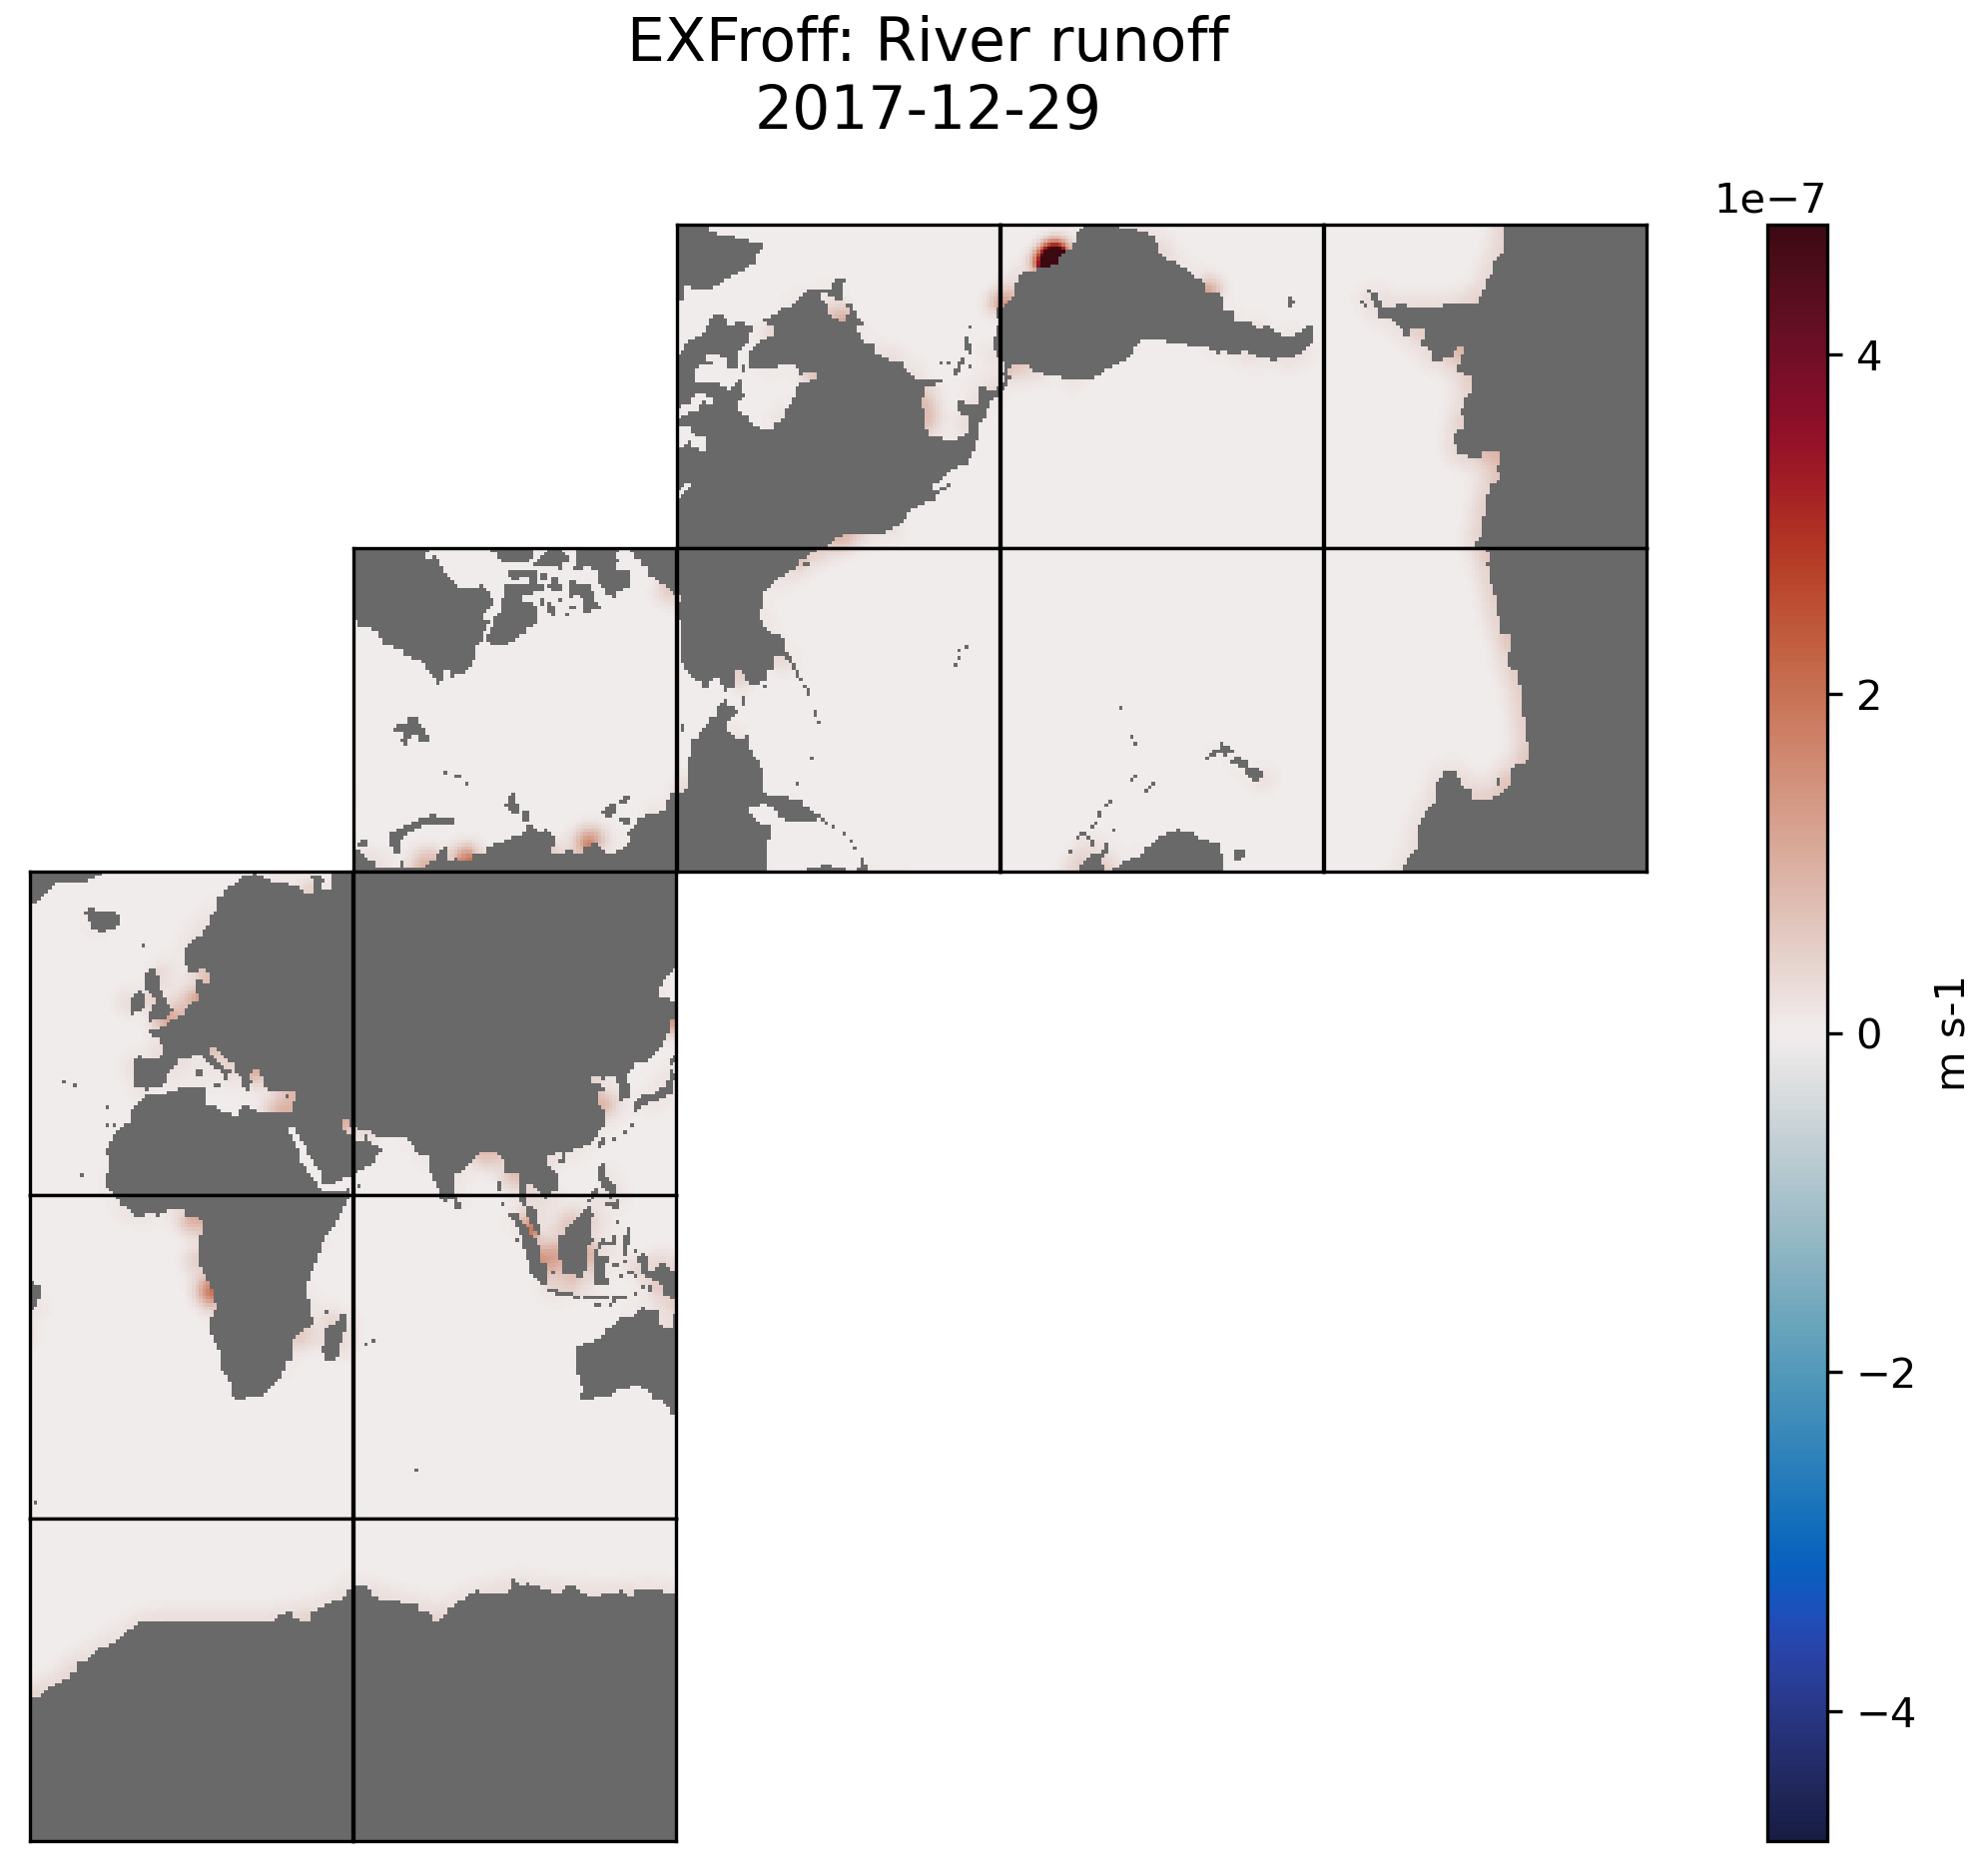
\includegraphics[scale=0.5]{../images/plots/native_plots/Ocean_and_Sea-Ice_Surface_Freshwater_Fluxes/EXFroff.png}
\caption{\\Dataset: OCEAN\_AND\_ICE\_SURFACE\_FW\_FLUX\\Variable: EXFroff}
\label{tab:table-OCEAN_AND_ICE_SURFACE_FW_FLUX_EXFroff-Plot}
\end{figure}
\pagebreak
\subsubsection{Native Variable SFLUX}
\begin{longtable}{|p{0.06\textwidth}|p{0.41\textwidth}|p{0.39\textwidth}|p{0.06\textwidth}|}
\caption{CDL description of OCEAN\_AND\_ICE\_SURFACE\_FW\_FLUX's SFLUX variable}
\label{tab:table-OCEAN_AND_ICE_SURFACE_FW_FLUX_SFLUX} \\ 
\hline \endhead \hline \endfoot
\rowcolor{lightgray} \textbf{Storage Type} & \textbf{Variable Name} & \textbf{Description} & \textbf{Unit} \\ \hline
float32 & SFLUX & Rate of change of total ocean salinity per m2 accounting for mass fluxes. & g m-2 s-1 \\ \hline
\rowcolor{lightgray}  \multicolumn{4}{|p{1.00\textwidth}|}{\textbf{CDL Description}} \\ \hline
\multicolumn{4}{|p{1.00\textwidth}|}{\makecell{\parbox{1\textwidth}{float32 SFLUX(time, tile, j, i)\\
\hspace*{0.5cm}SFLUX: \_FillValue = 9.96921e+36\\
\hspace*{0.5cm}SFLUX: long\_name = Rate of change of total ocean salinity per m2 accounting for mass fluxes.\\
\hspace*{0.5cm}SFLUX: units = g m: 2 s: 1\\
\hspace*{0.5cm}SFLUX: coverage\_content\_type = modelResult\\
\hspace*{0.5cm}SFLUX: direction = >0 increases salinity (SALT)\\
\hspace*{0.5cm}SFLUX: coordinates = YC XC time\\
\hspace*{0.5cm}SFLUX: valid\_min = : 0.07353577762842178\\
\hspace*{0.5cm}SFLUX: valid\_max = 0.010607733391225338}}} \\ \hline
\rowcolor{lightgray} \multicolumn{4}{|p{1.00\textwidth}|}{\textbf{Comments}} \\ \hline
\multicolumn{4}{|p{1\textwidth}|}{The rate of change of total ocean salinity due to freshwater fluxes across the liquid surface and the addition or removal of mass. Note: the global area integral of SFLUX matches the time-derivative of total ocean salinity (psu s-1). Unlike oceFWflx, SFLUX includes the contribution to the total ocean salinity from changing ocean mass (e.g. from the addition or removal of freshwater in oceFWflx). } \\ \hline
\end{longtable}

\begin{figure}[H]
\centering
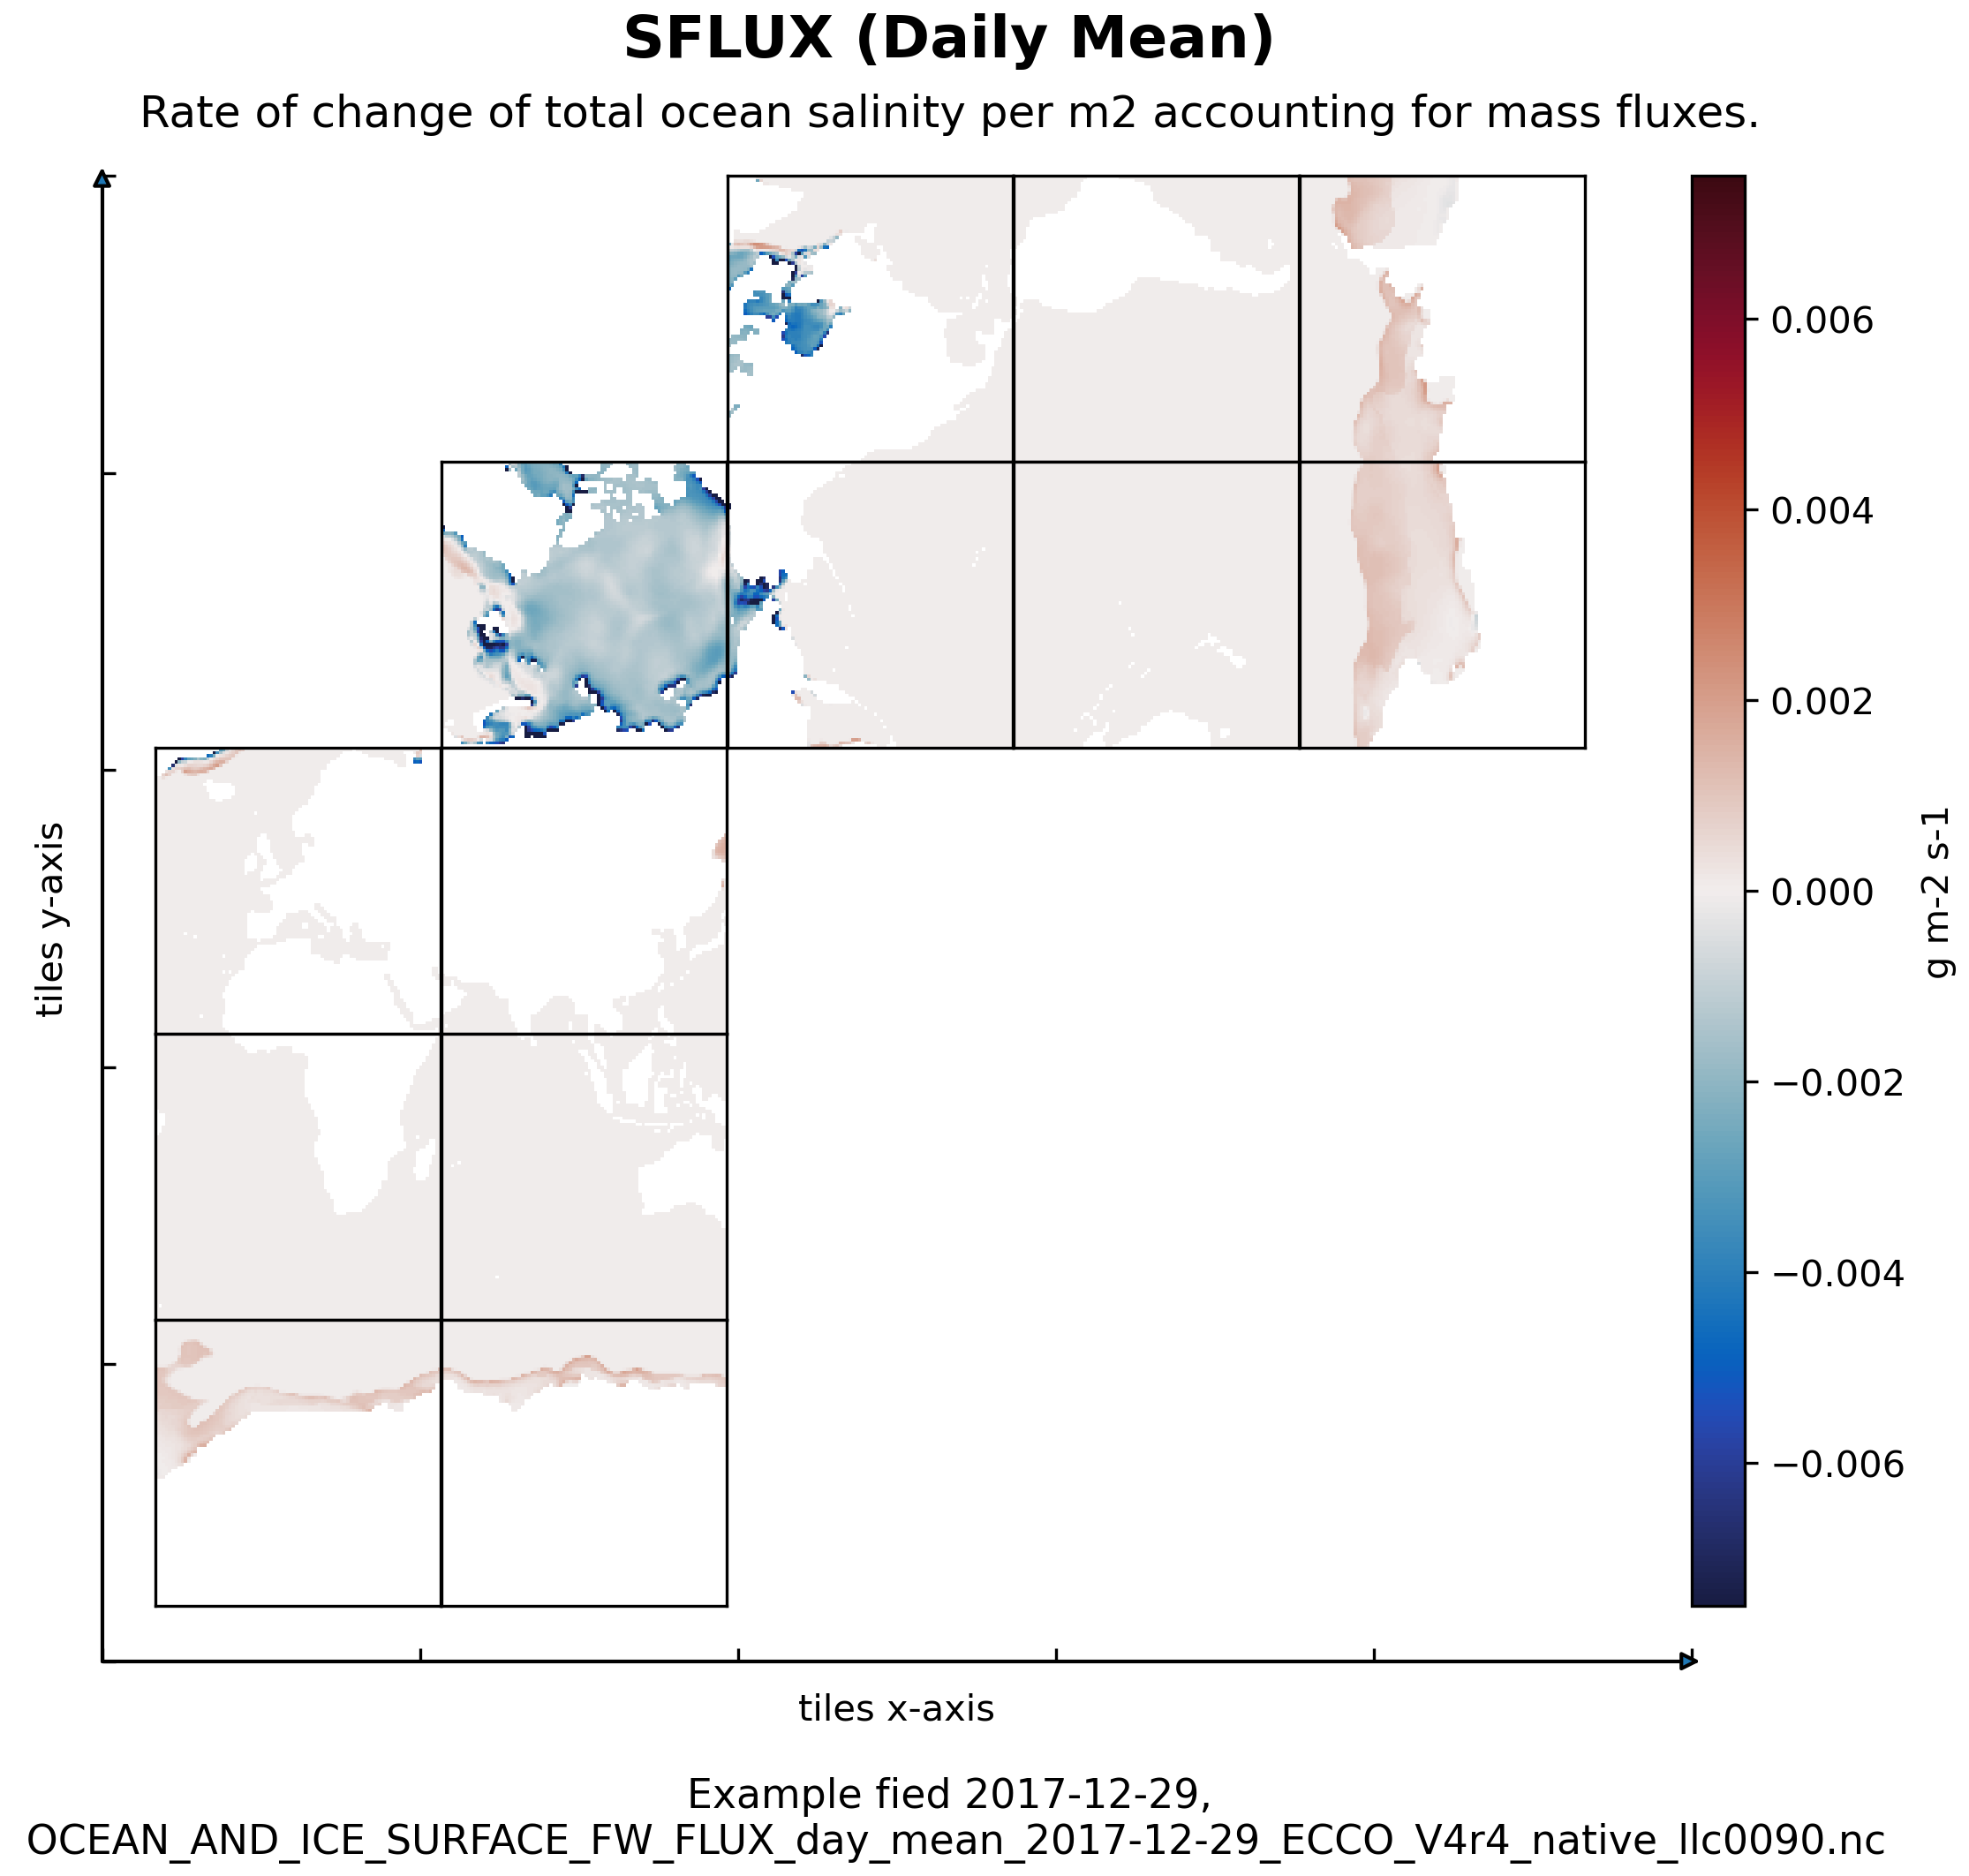
\includegraphics[scale=0.5]{../images/plots/native_plots/Ocean_and_Sea-Ice_Surface_Freshwater_Fluxes/SFLUX.png}
\caption{\\Dataset: OCEAN\_AND\_ICE\_SURFACE\_FW\_FLUX\\Variable: SFLUX}
\label{tab:table-OCEAN_AND_ICE_SURFACE_FW_FLUX_SFLUX-Plot}
\end{figure}
\pagebreak
\subsubsection{Native Variable SIacSubl}
\begin{longtable}{|p{0.06\textwidth}|p{0.41\textwidth}|p{0.39\textwidth}|p{0.06\textwidth}|}
\caption{CDL description of OCEAN\_AND\_ICE\_SURFACE\_FW\_FLUX's SIacSubl variable}
\label{tab:table-OCEAN_AND_ICE_SURFACE_FW_FLUX_SIacSubl} \\ 
\hline \endhead \hline \endfoot
\rowcolor{lightgray} \textbf{Storage Type} & \textbf{Variable Name} & \textbf{Description} & \textbf{Unit} \\ \hline
float32 & SIacSubl & Freshwater flux to the atmosphere due to sublimation-deposition of snow or ice & kg m-2 s-1 \\ \hline
\rowcolor{lightgray}  \multicolumn{4}{|p{1.00\textwidth}|}{\textbf{CDL Description}} \\ \hline
\multicolumn{4}{|p{1.00\textwidth}|}{\makecell{\parbox{1\textwidth}{float32 SIacSubl(time, tile, j, i)\\
\hspace*{0.5cm}SIacSubl: \_FillValue = 9.96921e+36\\
\hspace*{0.5cm}SIacSubl: long\_name = Freshwater flux to the atmosphere due to sublimation: deposition of snow or ice\\
\hspace*{0.5cm}SIacSubl: units = kg m: 2 s: 1\\
\hspace*{0.5cm}SIacSubl: coverage\_content\_type = modelResult\\
\hspace*{0.5cm}SIacSubl: direction = >0 decreases snow or sea: ice thickness (HSNOW or HEFF)\\
\hspace*{0.5cm}SIacSubl: standard\_name = water\_sublimation\_flux\\
\hspace*{0.5cm}SIacSubl: coordinates = YC XC time\\
\hspace*{0.5cm}SIacSubl: valid\_min = 0.0\\
\hspace*{0.5cm}SIacSubl: valid\_max = 8.154580427799374e: 05}}} \\ \hline
\rowcolor{lightgray} \multicolumn{4}{|p{1.00\textwidth}|}{\textbf{Comments}} \\ \hline
\multicolumn{4}{|p{1\textwidth}|}{Freshwater flux to the atmosphere due to sublimation-deposition of snow or ice. Positive values imply sublimation from ice/snow to vapor, negative values imply deposition from atmospheric moisture} \\ \hline
\end{longtable}

\begin{figure}[H]
\centering
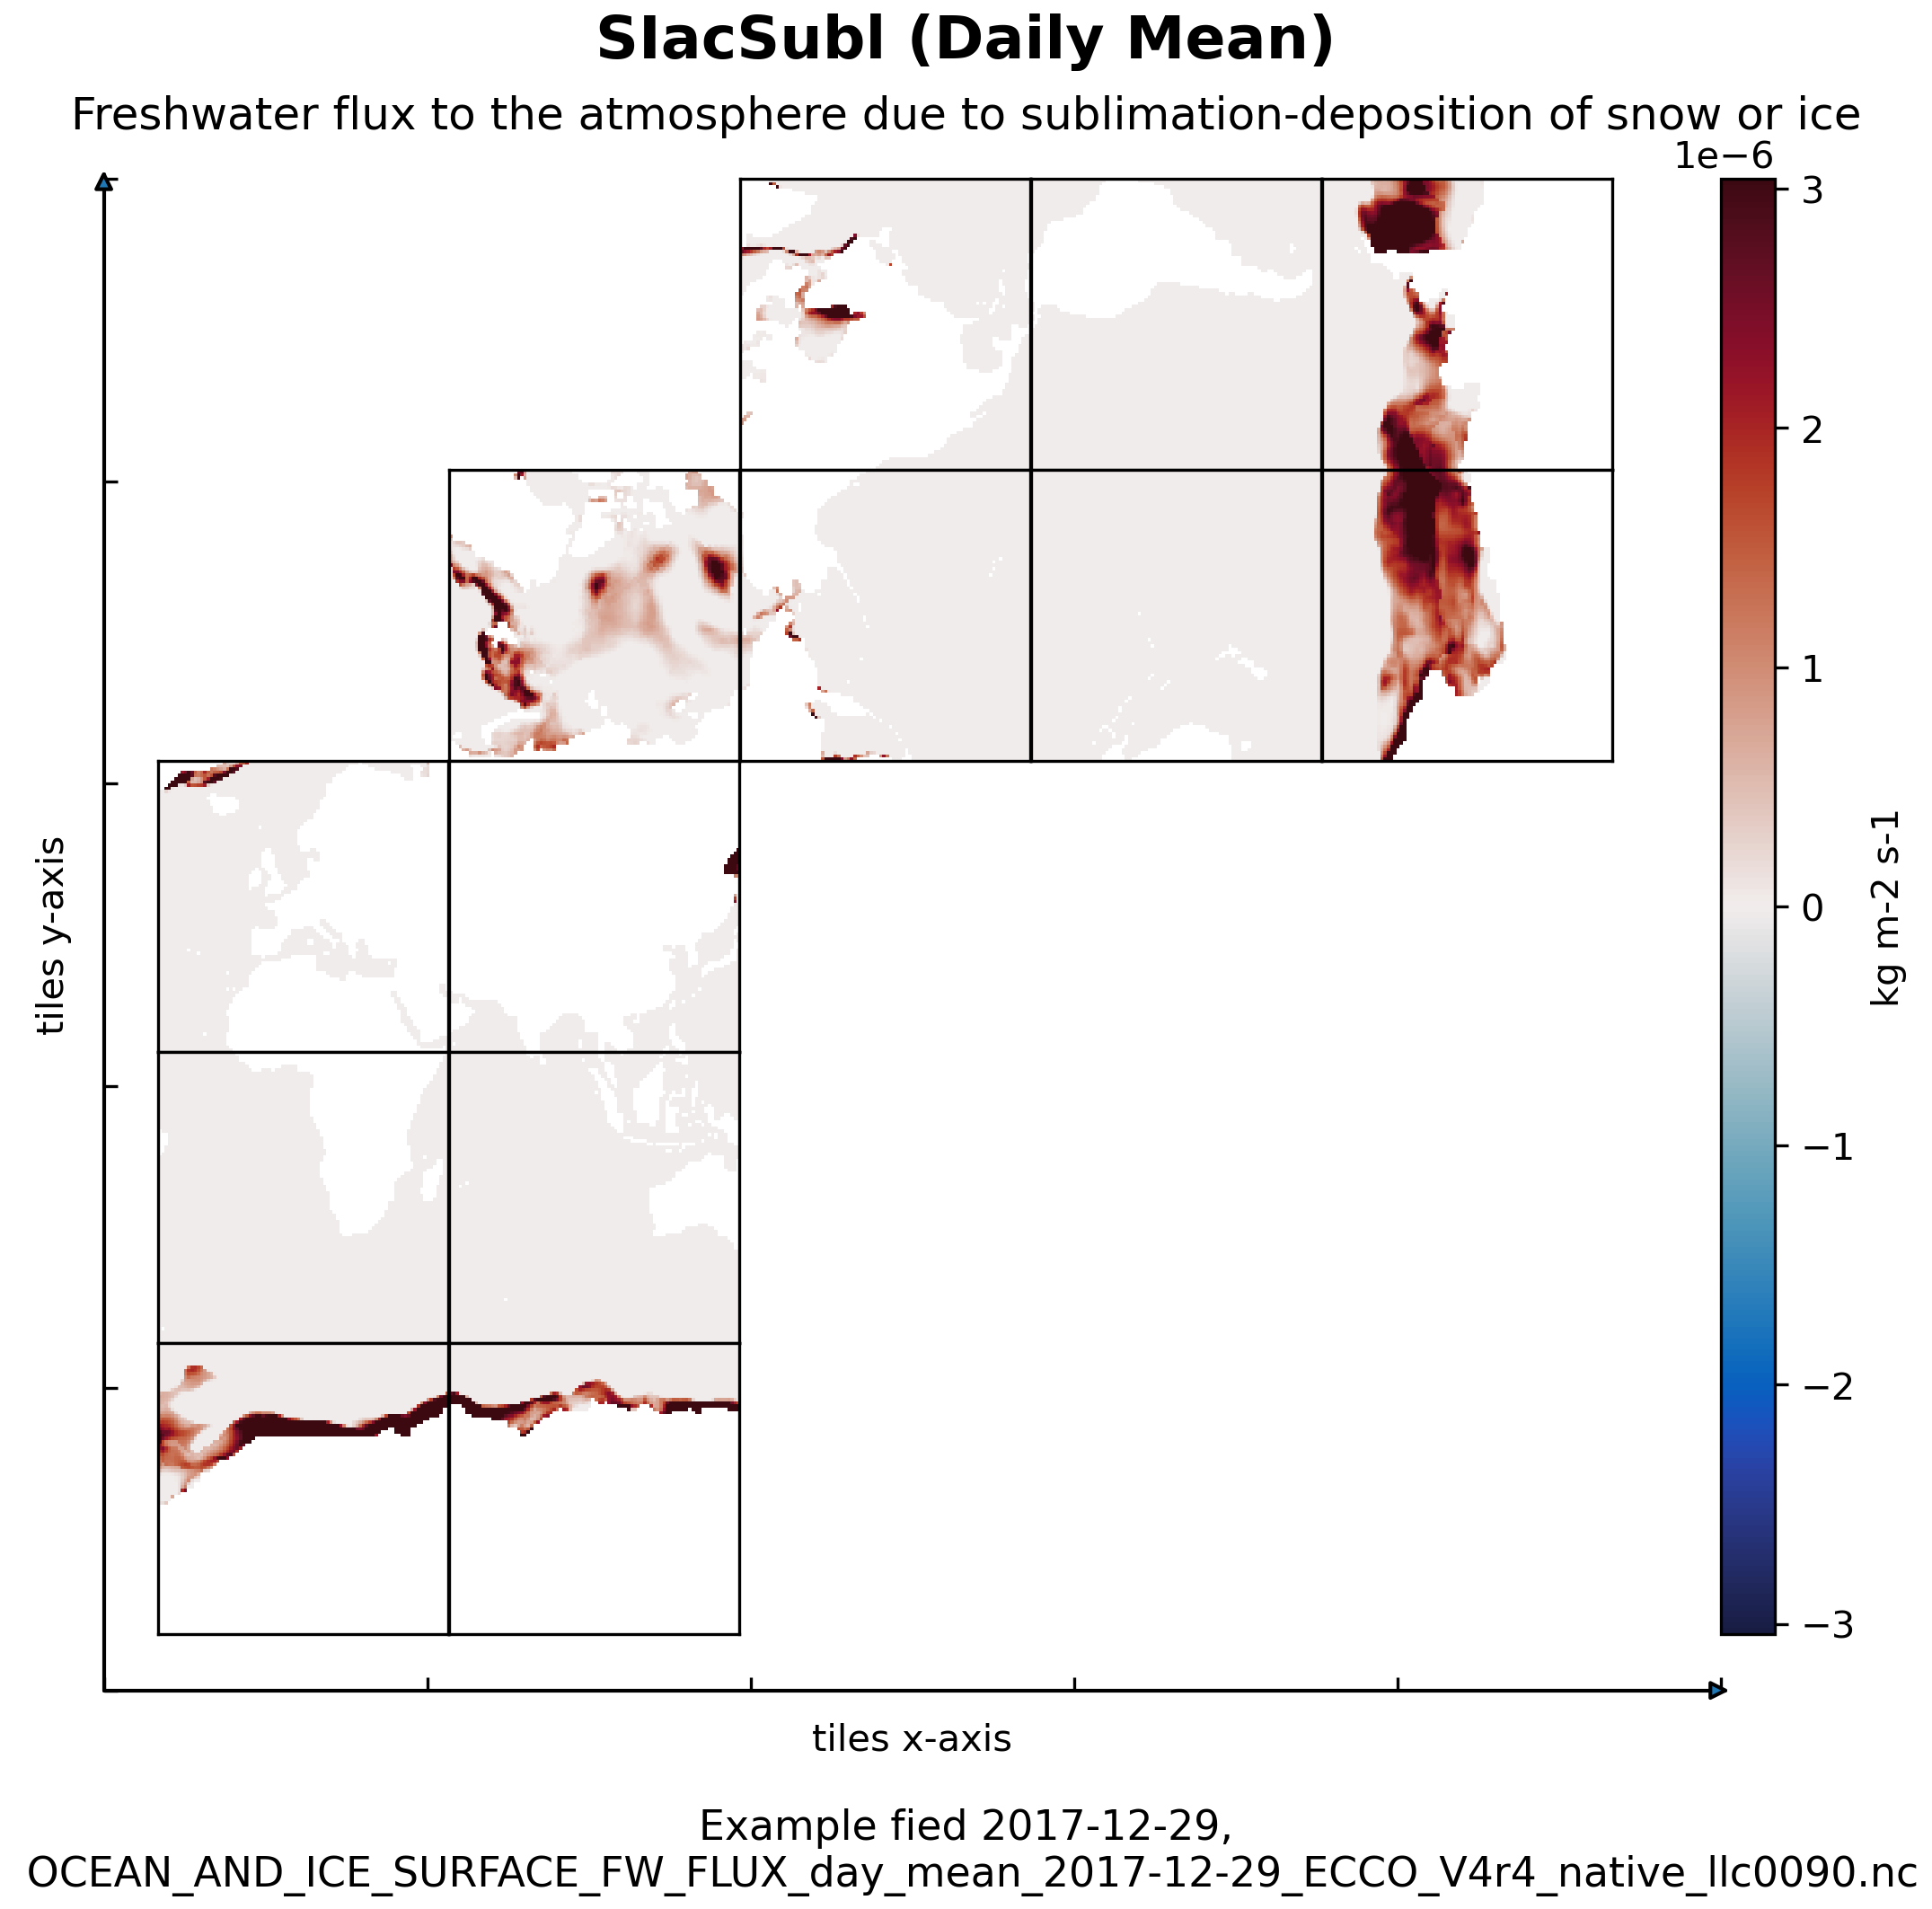
\includegraphics[scale=0.5]{../images/plots/native_plots/Ocean_and_Sea-Ice_Surface_Freshwater_Fluxes/SIacSubl.png}
\caption{\\Dataset: OCEAN\_AND\_ICE\_SURFACE\_FW\_FLUX\\Variable: SIacSubl}
\label{tab:table-OCEAN_AND_ICE_SURFACE_FW_FLUX_SIacSubl-Plot}
\end{figure}
\pagebreak
\subsubsection{Native Variable SIatmFW}
\begin{longtable}{|p{0.06\textwidth}|p{0.41\textwidth}|p{0.39\textwidth}|p{0.06\textwidth}|}
\caption{CDL description of OCEAN\_AND\_ICE\_SURFACE\_FW\_FLUX's SIatmFW variable}
\label{tab:table-OCEAN_AND_ICE_SURFACE_FW_FLUX_SIatmFW} \\ 
\hline \endhead \hline \endfoot
\rowcolor{lightgray} \textbf{Storage Type} & \textbf{Variable Name} & \textbf{Description} & \textbf{Unit} \\ \hline
float32 & SIatmFW & Net freshwater flux into the open ocean, sea-ice, and snow & kg m-2 s-1 \\ \hline
\rowcolor{lightgray}  \multicolumn{4}{|p{1.00\textwidth}|}{\textbf{CDL Description}} \\ \hline
\multicolumn{4}{|p{1.00\textwidth}|}{\makecell{\parbox{1\textwidth}{float32 SIatmFW(time, tile, j, i)\\
\hspace*{0.5cm}SIatmFW: \_FillValue = 9.96921e+36\\
\hspace*{0.5cm}SIatmFW: long\_name = Net freshwater flux into the open ocean\\
sea: ice\\
and snow\\
\hspace*{0.5cm}SIatmFW: units = kg m: 2 s: 1\\
\hspace*{0.5cm}SIatmFW: coverage\_content\_type = modelResult\\
\hspace*{0.5cm}SIatmFW: direction = >0 decreases salinity (SALT)\\
\hspace*{0.5cm}SIatmFW: standard\_name = surface\_downward\_water\_flux\\
\hspace*{0.5cm}SIatmFW: coordinates = YC XC time\\
\hspace*{0.5cm}SIatmFW: valid\_min = : 0.00043017856660299003\\
\hspace*{0.5cm}SIatmFW: valid\_max = 0.008299433626234531}}} \\ \hline
\rowcolor{lightgray} \multicolumn{4}{|p{1.00\textwidth}|}{\textbf{Comments}} \\ \hline
\multicolumn{4}{|p{1\textwidth}|}{Net freshwater flux into the combined liquid ocean, sea-ice, and snow reservoirs from the atmosphere and runoff. Note: freshwater fluxes BETWEEN the liquid ocean and sea-ice or snow reservoirs do not contribute to SIatmFW. SIatmFW counts all fluxes to/from the atmosphere that change the TOTAL freshwater stored in the combined liquid ocean, sea-ice, and snow reservoirs.} \\ \hline
\end{longtable}

\begin{figure}[H]
\centering
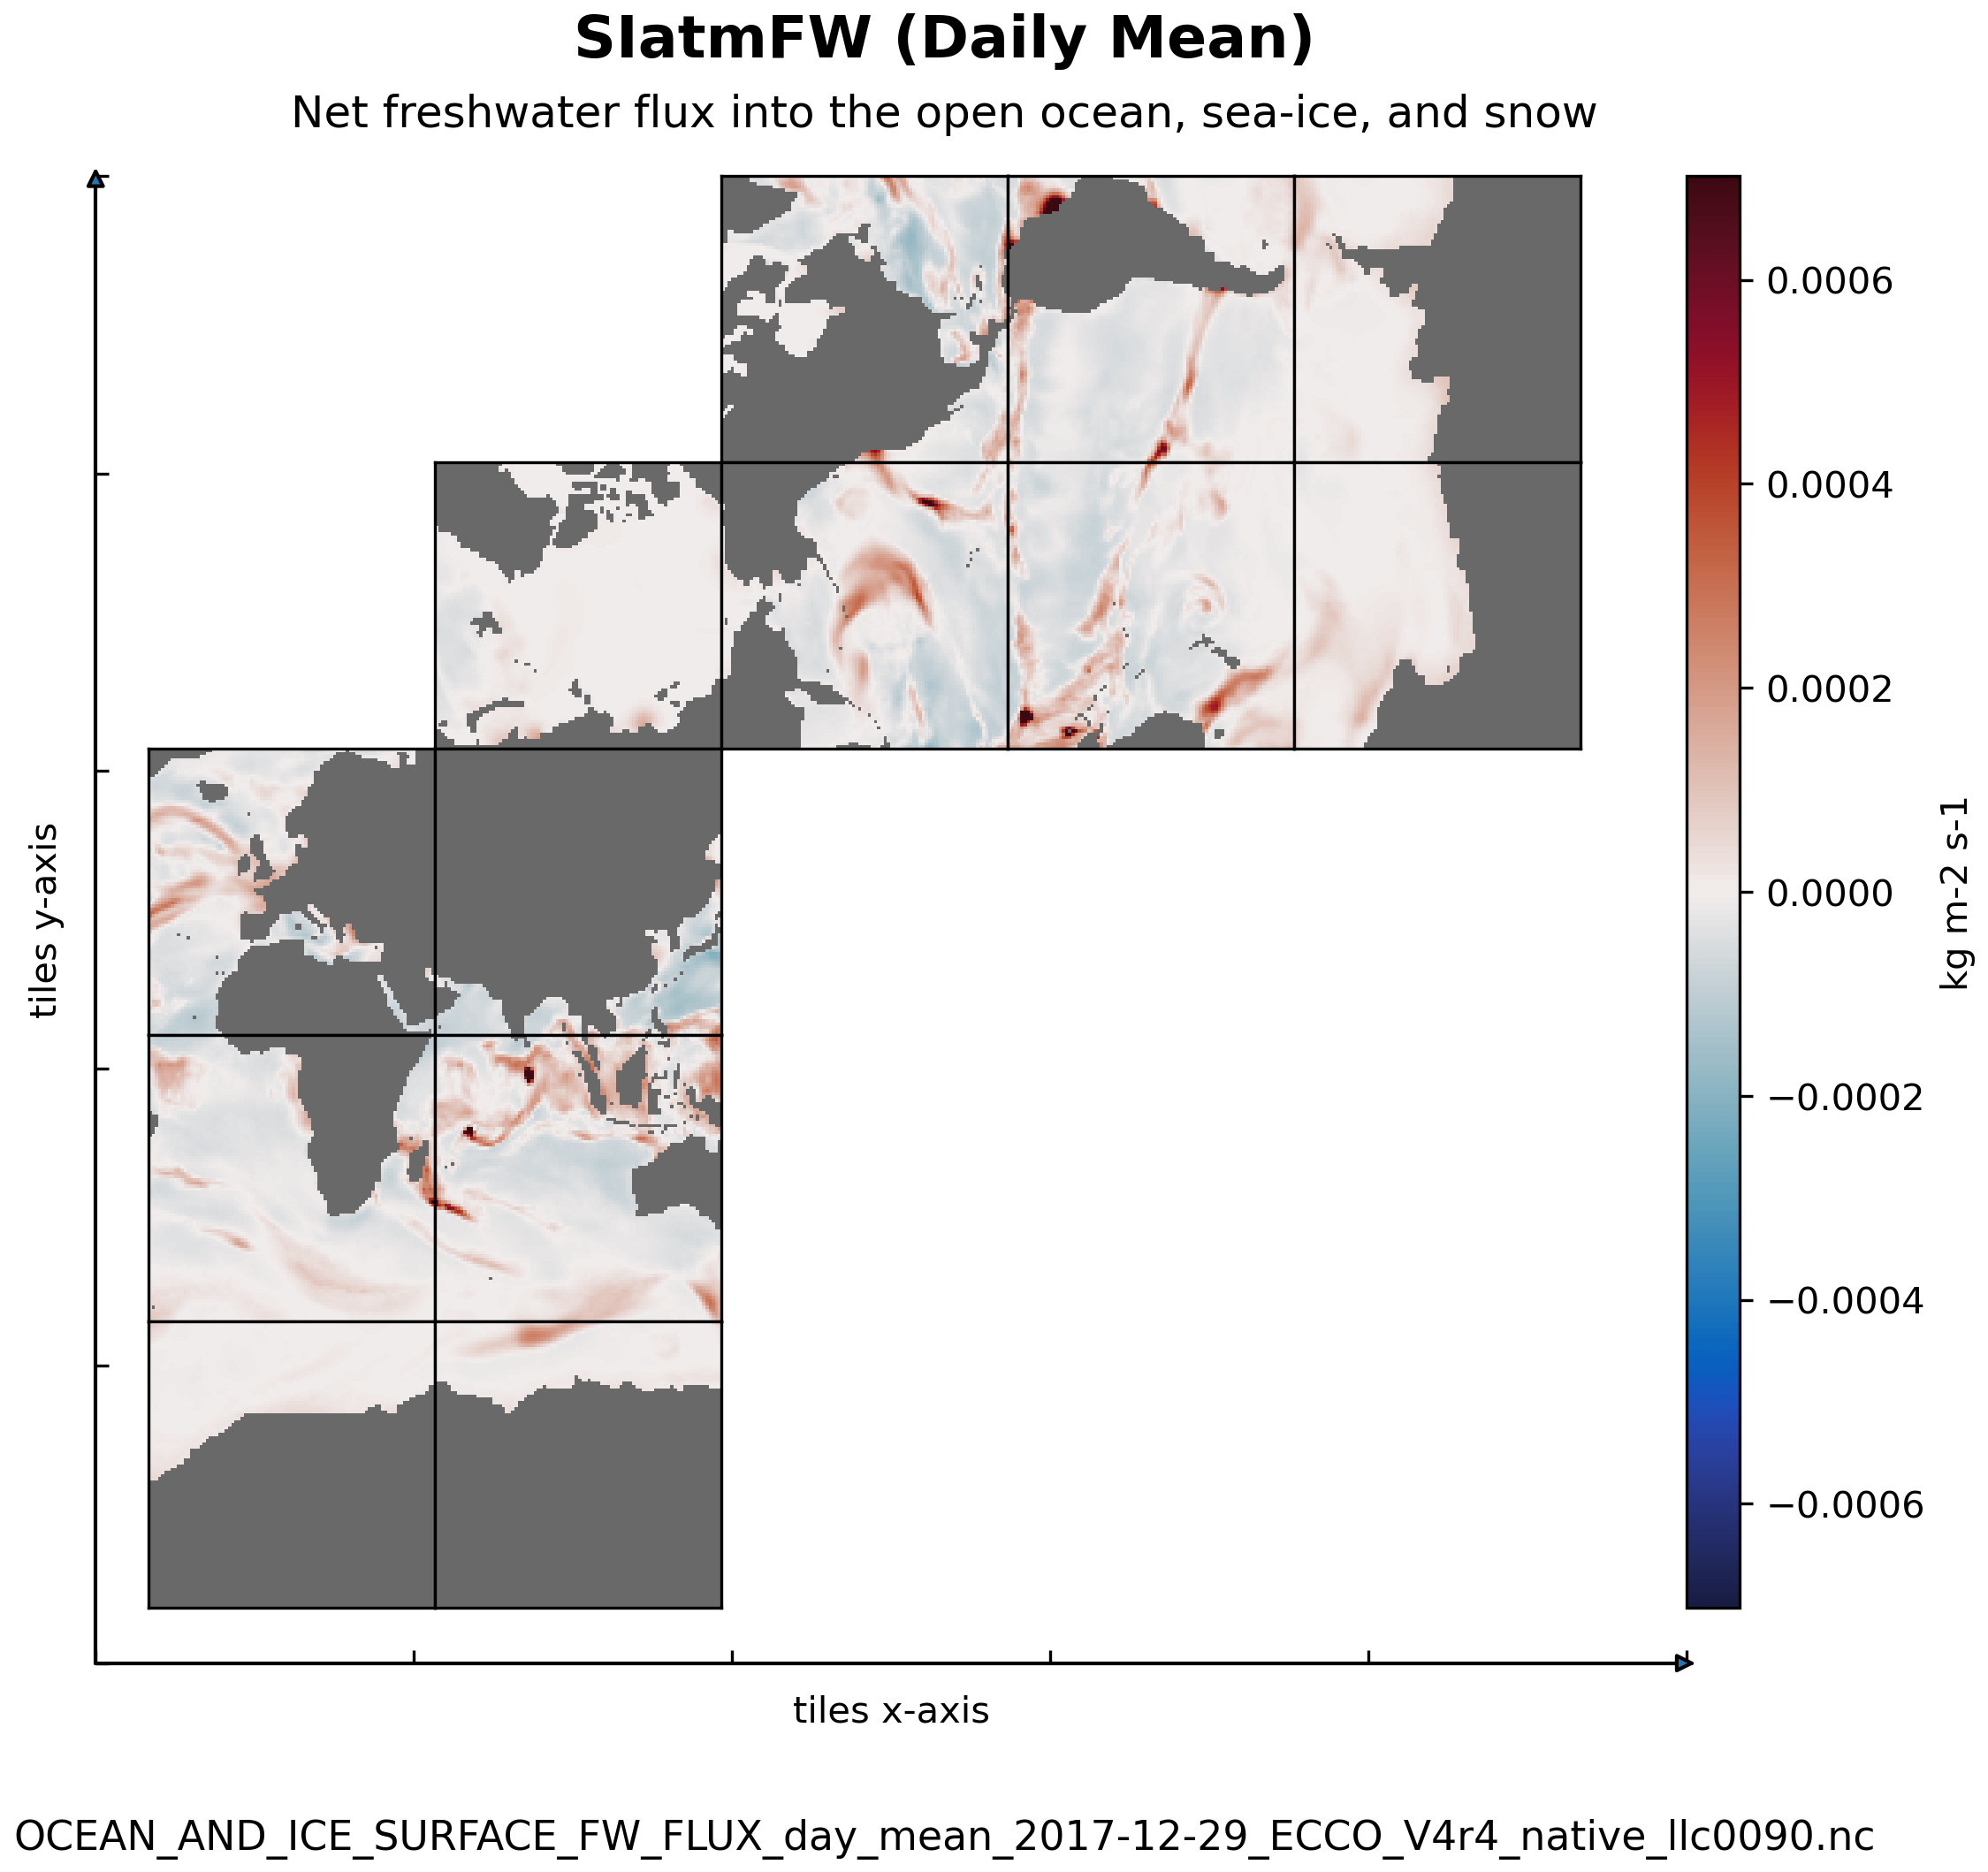
\includegraphics[scale=0.5]{../images/plots/native_plots/Ocean_and_Sea-Ice_Surface_Freshwater_Fluxes/SIatmFW.png}
\caption{\\Dataset: OCEAN\_AND\_ICE\_SURFACE\_FW\_FLUX\\Variable: SIatmFW}
\label{tab:table-OCEAN_AND_ICE_SURFACE_FW_FLUX_SIatmFW-Plot}
\end{figure}
\pagebreak
\subsubsection{Native Variable SIfwThru}
\begin{longtable}{|p{0.06\textwidth}|p{0.41\textwidth}|p{0.39\textwidth}|p{0.06\textwidth}|}
\caption{CDL description of OCEAN\_AND\_ICE\_SURFACE\_FW\_FLUX's SIfwThru variable}
\label{tab:table-OCEAN_AND_ICE_SURFACE_FW_FLUX_SIfwThru} \\ 
\hline \endhead \hline \endfoot
\rowcolor{lightgray} \textbf{Storage Type} & \textbf{Variable Name} & \textbf{Description} & \textbf{Unit} \\ \hline
float32 & SIfwThru & Precipitation through sea-ice & kg m-2 s-1 \\ \hline
\rowcolor{lightgray}  \multicolumn{4}{|p{1.00\textwidth}|}{\textbf{CDL Description}} \\ \hline
\multicolumn{4}{|p{1.00\textwidth}|}{\makecell{\parbox{1\textwidth}{float32 SIfwThru(time, tile, j, i)\\
\hspace*{0.5cm}SIfwThru: \_FillValue = 9.96921e+36\\
\hspace*{0.5cm}SIfwThru: long\_name = Precipitation through sea: ice\\
\hspace*{0.5cm}SIfwThru: units = kg m: 2 s: 1\\
\hspace*{0.5cm}SIfwThru: coverage\_content\_type = modelResult\\
\hspace*{0.5cm}SIfwThru: direction = >0 increases ocean volume\\
\hspace*{0.5cm}SIfwThru: coordinates = YC XC time\\
\hspace*{0.5cm}SIfwThru: valid\_min = : 1.695218452368863e: 05\\
\hspace*{0.5cm}SIfwThru: valid\_max = 0.0010632629273459315}}} \\ \hline
\rowcolor{lightgray} \multicolumn{4}{|p{1.00\textwidth}|}{\textbf{Comments}} \\ \hline
\multicolumn{4}{|p{1\textwidth}|}{Precipitation over sea-ice covered regions reaching ocean through sea-ice. Note: Precipitation over sea-ice covered regions that directly reaches ocean through the sea-ice. It is not due to melt of sea-ice/snow.} \\ \hline
\end{longtable}

\begin{figure}[H]
\centering
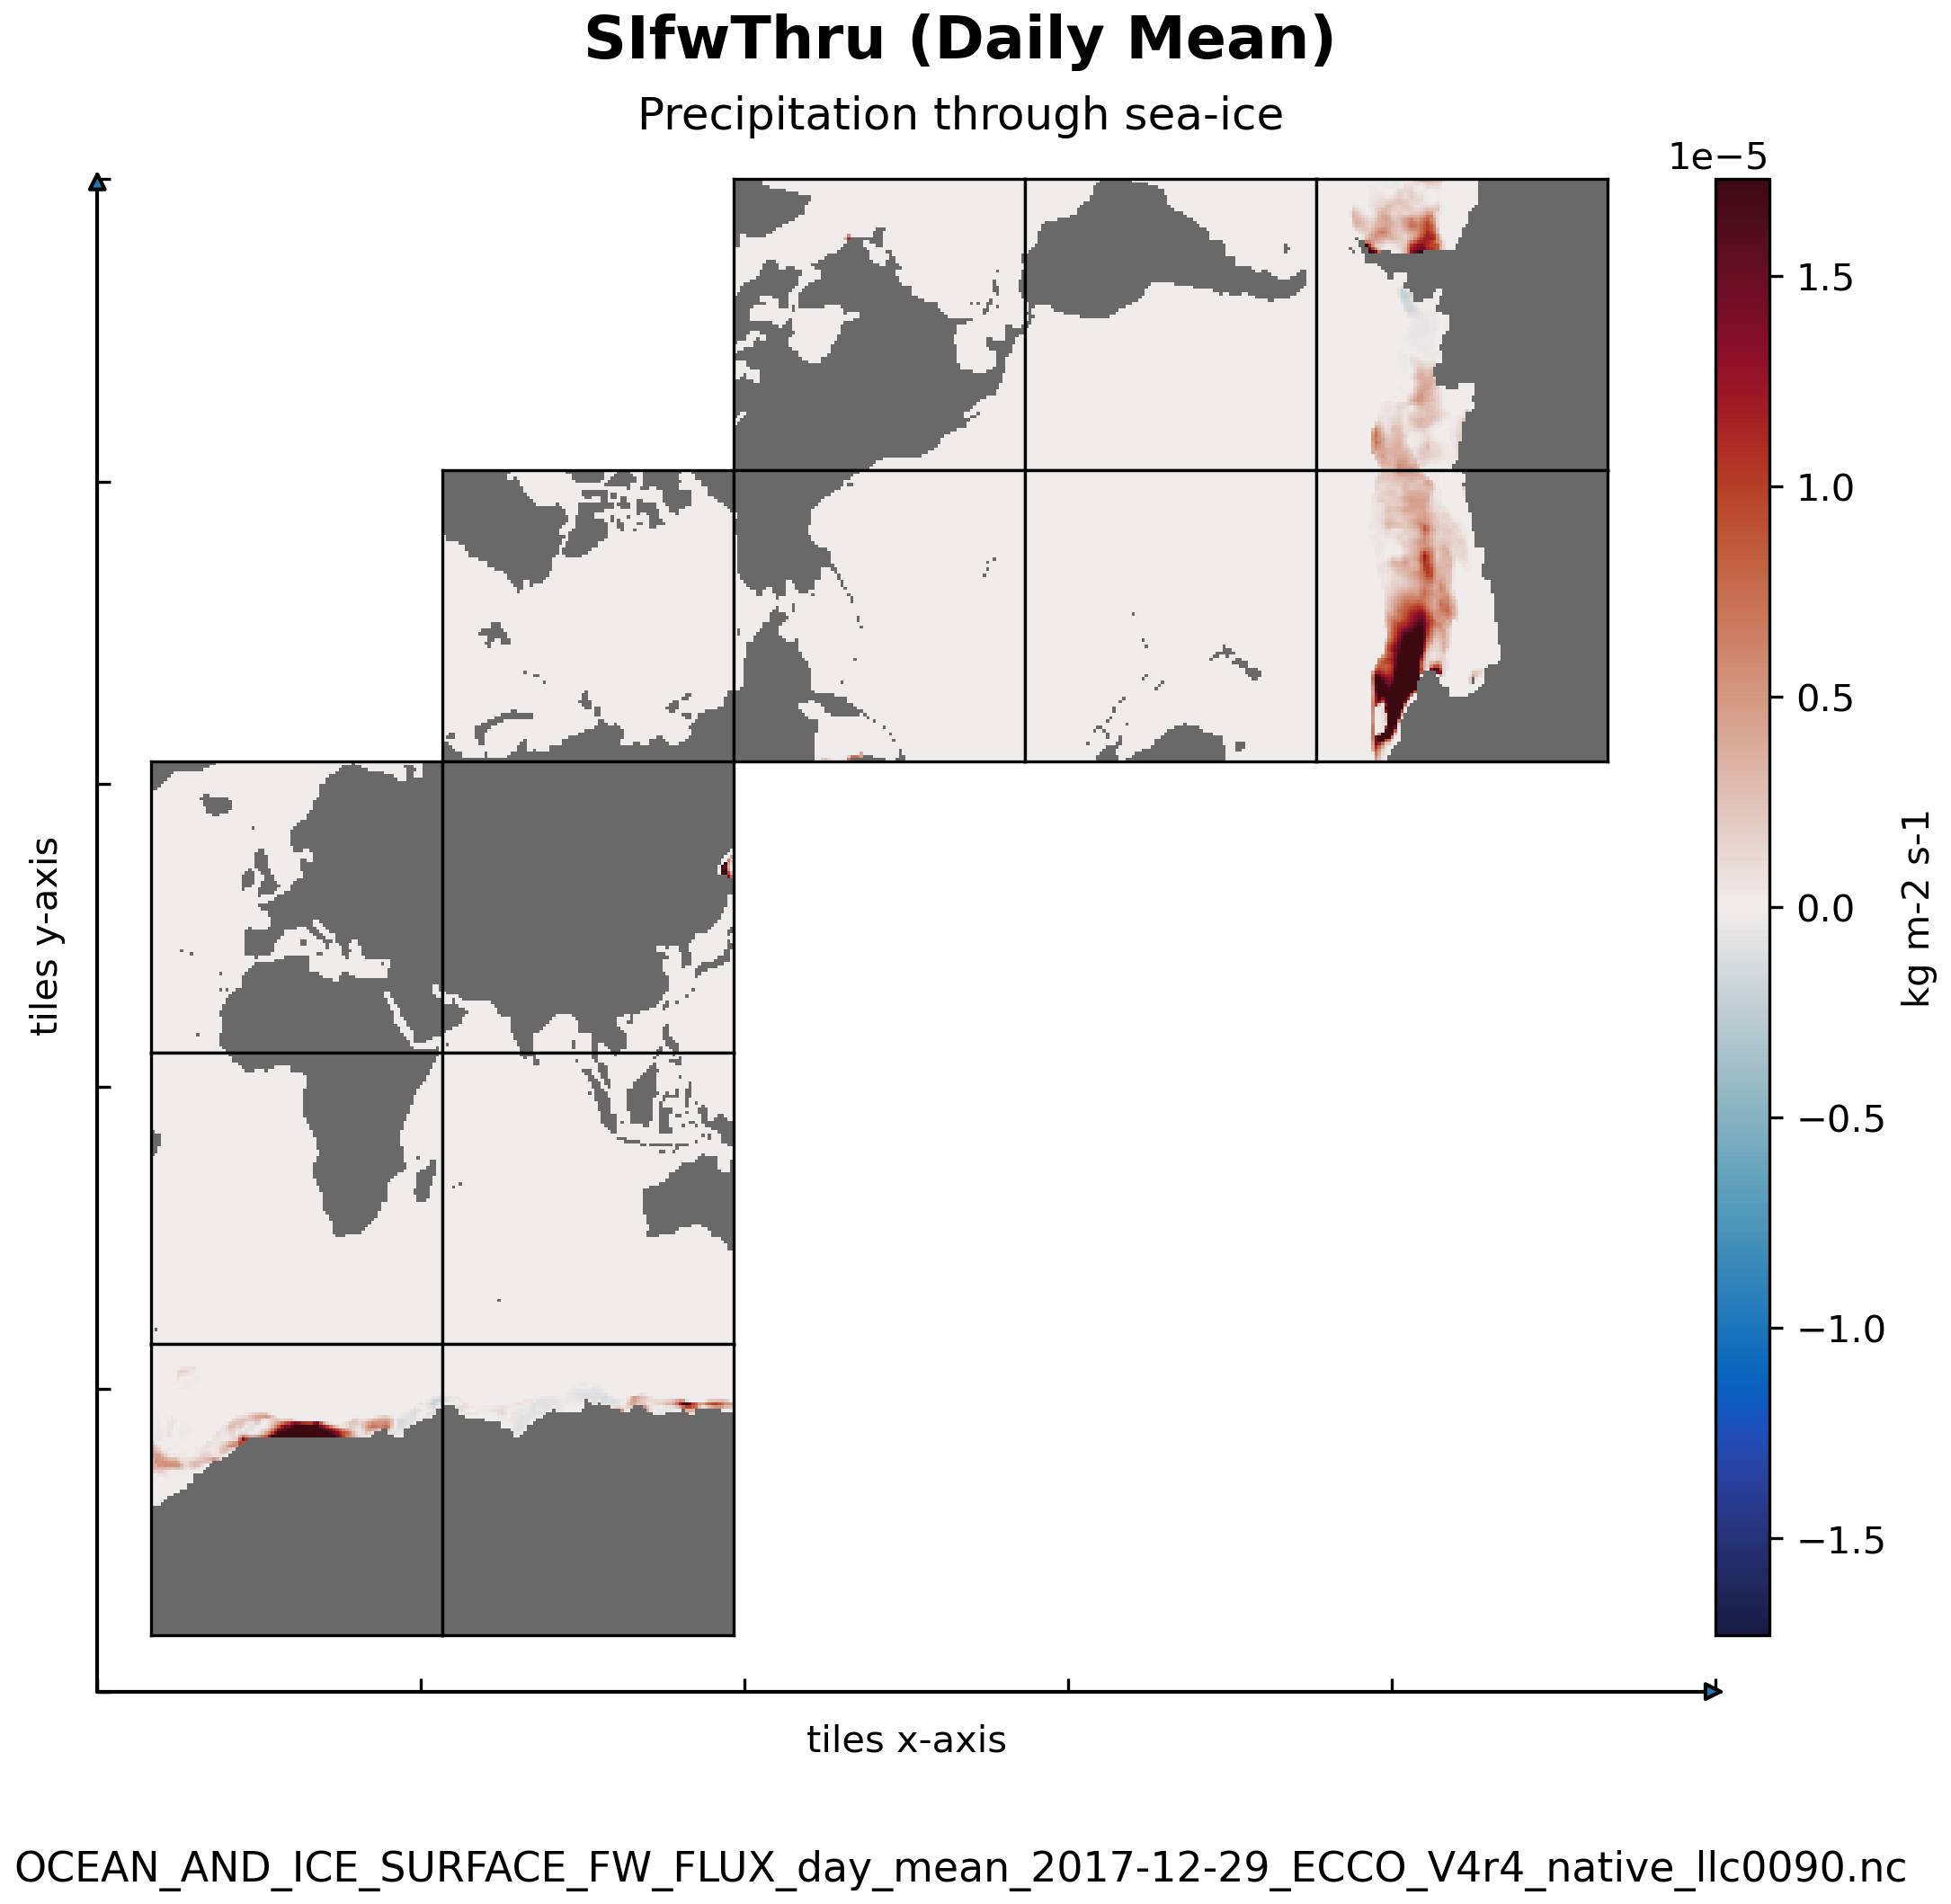
\includegraphics[scale=0.5]{../images/plots/native_plots/Ocean_and_Sea-Ice_Surface_Freshwater_Fluxes/SIfwThru.png}
\caption{\\Dataset: OCEAN\_AND\_ICE\_SURFACE\_FW\_FLUX\\Variable: SIfwThru}
\label{tab:table-OCEAN_AND_ICE_SURFACE_FW_FLUX_SIfwThru-Plot}
\end{figure}
\pagebreak
\subsubsection{Native Variable SIrsSubl}
\begin{longtable}{|p{0.06\textwidth}|p{0.41\textwidth}|p{0.39\textwidth}|p{0.06\textwidth}|}
\caption{CDL description of OCEAN\_AND\_ICE\_SURFACE\_FW\_FLUX's SIrsSubl variable}
\label{tab:table-OCEAN_AND_ICE_SURFACE_FW_FLUX_SIrsSubl} \\ 
\hline \endhead \hline \endfoot
\rowcolor{lightgray} \textbf{Storage Type} & \textbf{Variable Name} & \textbf{Description} & \textbf{Unit} \\ \hline
float32 & SIrsSubl & Residual sublimation freshwater flux & kg m-2 s-1 \\ \hline
\rowcolor{lightgray}  \multicolumn{4}{|p{1.00\textwidth}|}{\textbf{CDL Description}} \\ \hline
\multicolumn{4}{|p{1.00\textwidth}|}{\makecell{\parbox{1\textwidth}{float32 SIrsSubl(time, tile, j, i)\\
\hspace*{0.5cm}SIrsSubl: \_FillValue = 9.96921e+36\\
\hspace*{0.5cm}SIrsSubl: long\_name = Residual sublimation freshwater flux\\
\hspace*{0.5cm}SIrsSubl: units = kg m: 2 s: 1\\
\hspace*{0.5cm}SIrsSubl: coverage\_content\_type = modelResult\\
\hspace*{0.5cm}SIrsSubl: direction = >0 decreases ocean volume\\
\hspace*{0.5cm}SIrsSubl: coordinates = YC XC time\\
\hspace*{0.5cm}SIrsSubl: valid\_min = : 0.0001067528864950873\\
\hspace*{0.5cm}SIrsSubl: valid\_max = 8.640533451398369e: 06}}} \\ \hline
\rowcolor{lightgray} \multicolumn{4}{|p{1.00\textwidth}|}{\textbf{Comments}} \\ \hline
\multicolumn{4}{|p{1\textwidth}|}{Residual freshwater flux by sublimation to remove water from or add water to ocean. When implied sublimation freshwater flux SIacSubl is larger than availabe sea-ice/snow, SIrsSubl is positive and water is removed from ocean. Note: freshwater flux by sublimation that is to remove water from the ocean when it is positive.} \\ \hline
\end{longtable}

\begin{figure}[H]
\centering
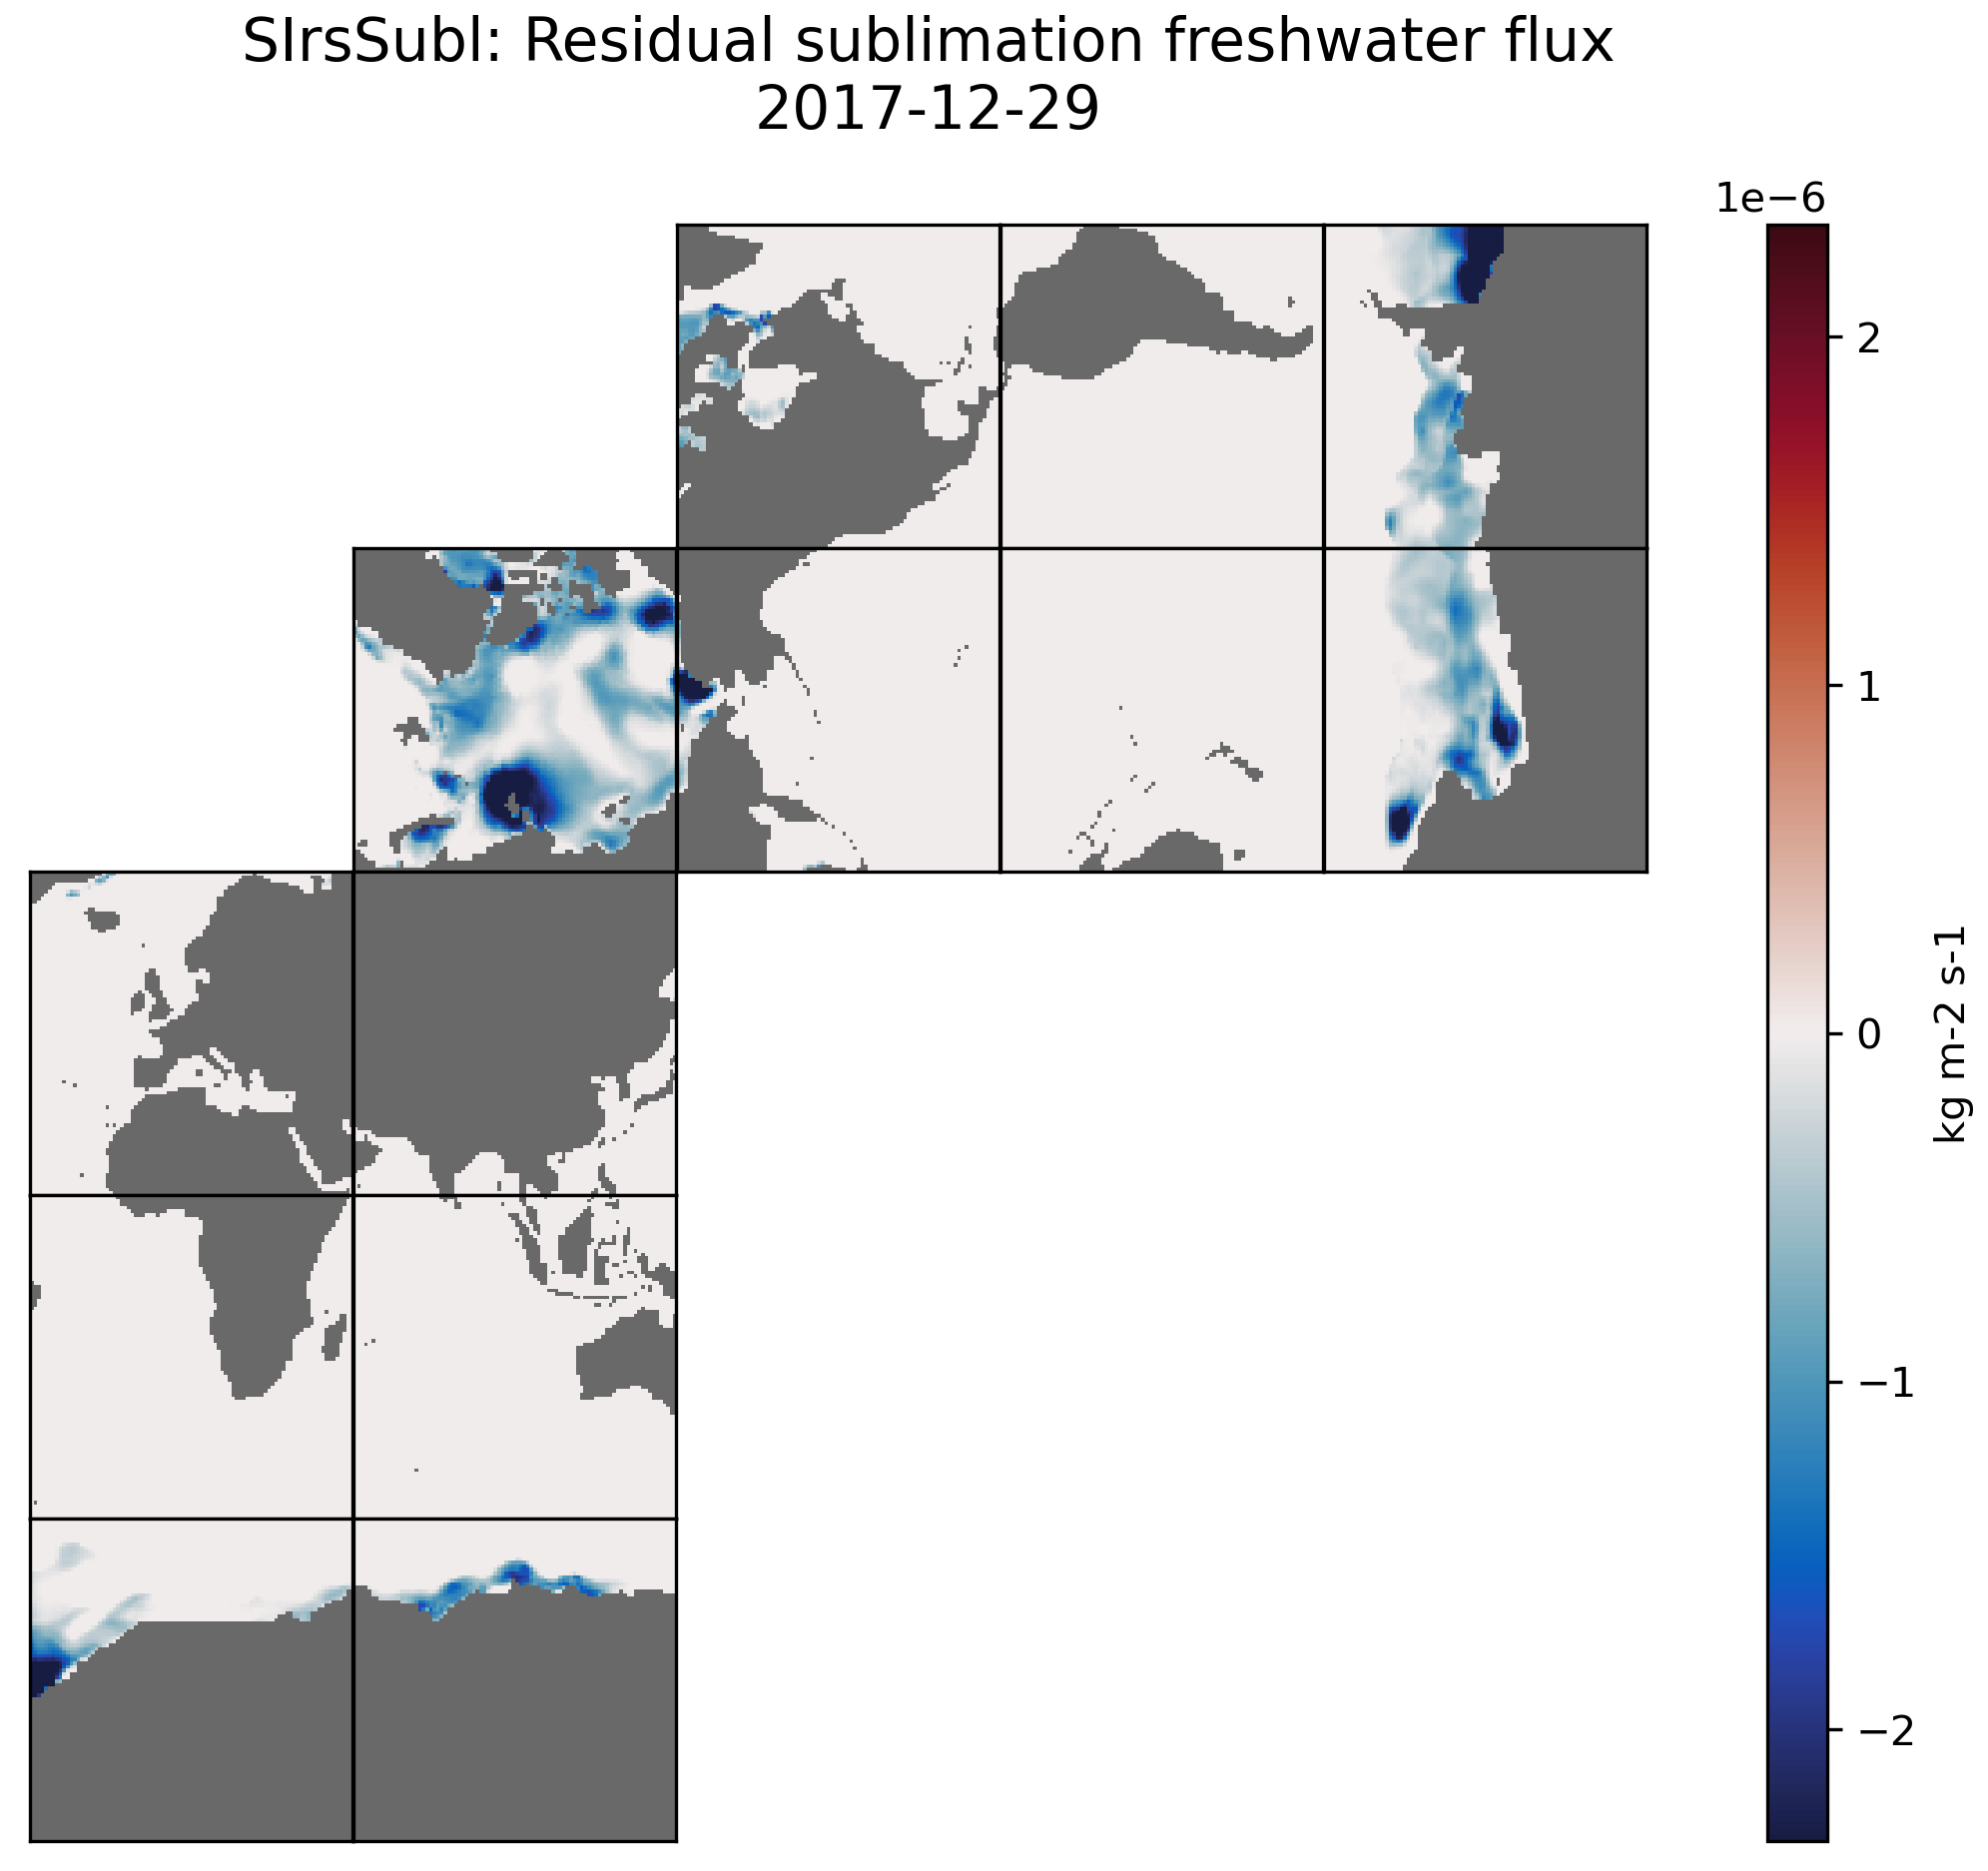
\includegraphics[scale=0.5]{../images/plots/native_plots/Ocean_and_Sea-Ice_Surface_Freshwater_Fluxes/SIrsSubl.png}
\caption{\\Dataset: OCEAN\_AND\_ICE\_SURFACE\_FW\_FLUX\\Variable: SIrsSubl}
\label{tab:table-OCEAN_AND_ICE_SURFACE_FW_FLUX_SIrsSubl-Plot}
\end{figure}
\pagebreak
\subsubsection{Native Variable SIsnPrcp}
\begin{longtable}{|p{0.06\textwidth}|p{0.41\textwidth}|p{0.39\textwidth}|p{0.06\textwidth}|}
\caption{CDL description of OCEAN\_AND\_ICE\_SURFACE\_FW\_FLUX's SIsnPrcp variable}
\label{tab:table-OCEAN_AND_ICE_SURFACE_FW_FLUX_SIsnPrcp} \\ 
\hline \endhead \hline \endfoot
\rowcolor{lightgray} \textbf{Storage Type} & \textbf{Variable Name} & \textbf{Description} & \textbf{Unit} \\ \hline
float32 & SIsnPrcp & Snow precipitation on sea-ice & kg m-2 s-1 \\ \hline
\rowcolor{lightgray}  \multicolumn{4}{|p{1.00\textwidth}|}{\textbf{CDL Description}} \\ \hline
\multicolumn{4}{|p{1.00\textwidth}|}{\makecell{\parbox{1\textwidth}{float32 SIsnPrcp(time, tile, j, i)\\
\hspace*{0.5cm}SIsnPrcp: \_FillValue = 9.96921e+36\\
\hspace*{0.5cm}SIsnPrcp: long\_name = Snow precipitation on sea: ice\\
\hspace*{0.5cm}SIsnPrcp: units = kg m: 2 s: 1\\
\hspace*{0.5cm}SIsnPrcp: coverage\_content\_type = modelResult\\
\hspace*{0.5cm}SIsnPrcp: direction = >0 increases snow thickness (HSNOW)\\
\hspace*{0.5cm}SIsnPrcp: standard\_name = snowfall\_flux\\
\hspace*{0.5cm}SIsnPrcp: coordinates = YC XC time\\
\hspace*{0.5cm}SIsnPrcp: valid\_min = : 4.334669574745931e: 05\\
\hspace*{0.5cm}SIsnPrcp: valid\_max = 0.0009354020585305989}}} \\ \hline
\rowcolor{lightgray} \multicolumn{4}{|p{1.00\textwidth}|}{\textbf{Comments}} \\ \hline
\multicolumn{4}{|p{1\textwidth}|}{Snow precipitation rate over sea-ice, averaged over the entire model grid cell.} \\ \hline
\end{longtable}

\begin{figure}[H]
\centering
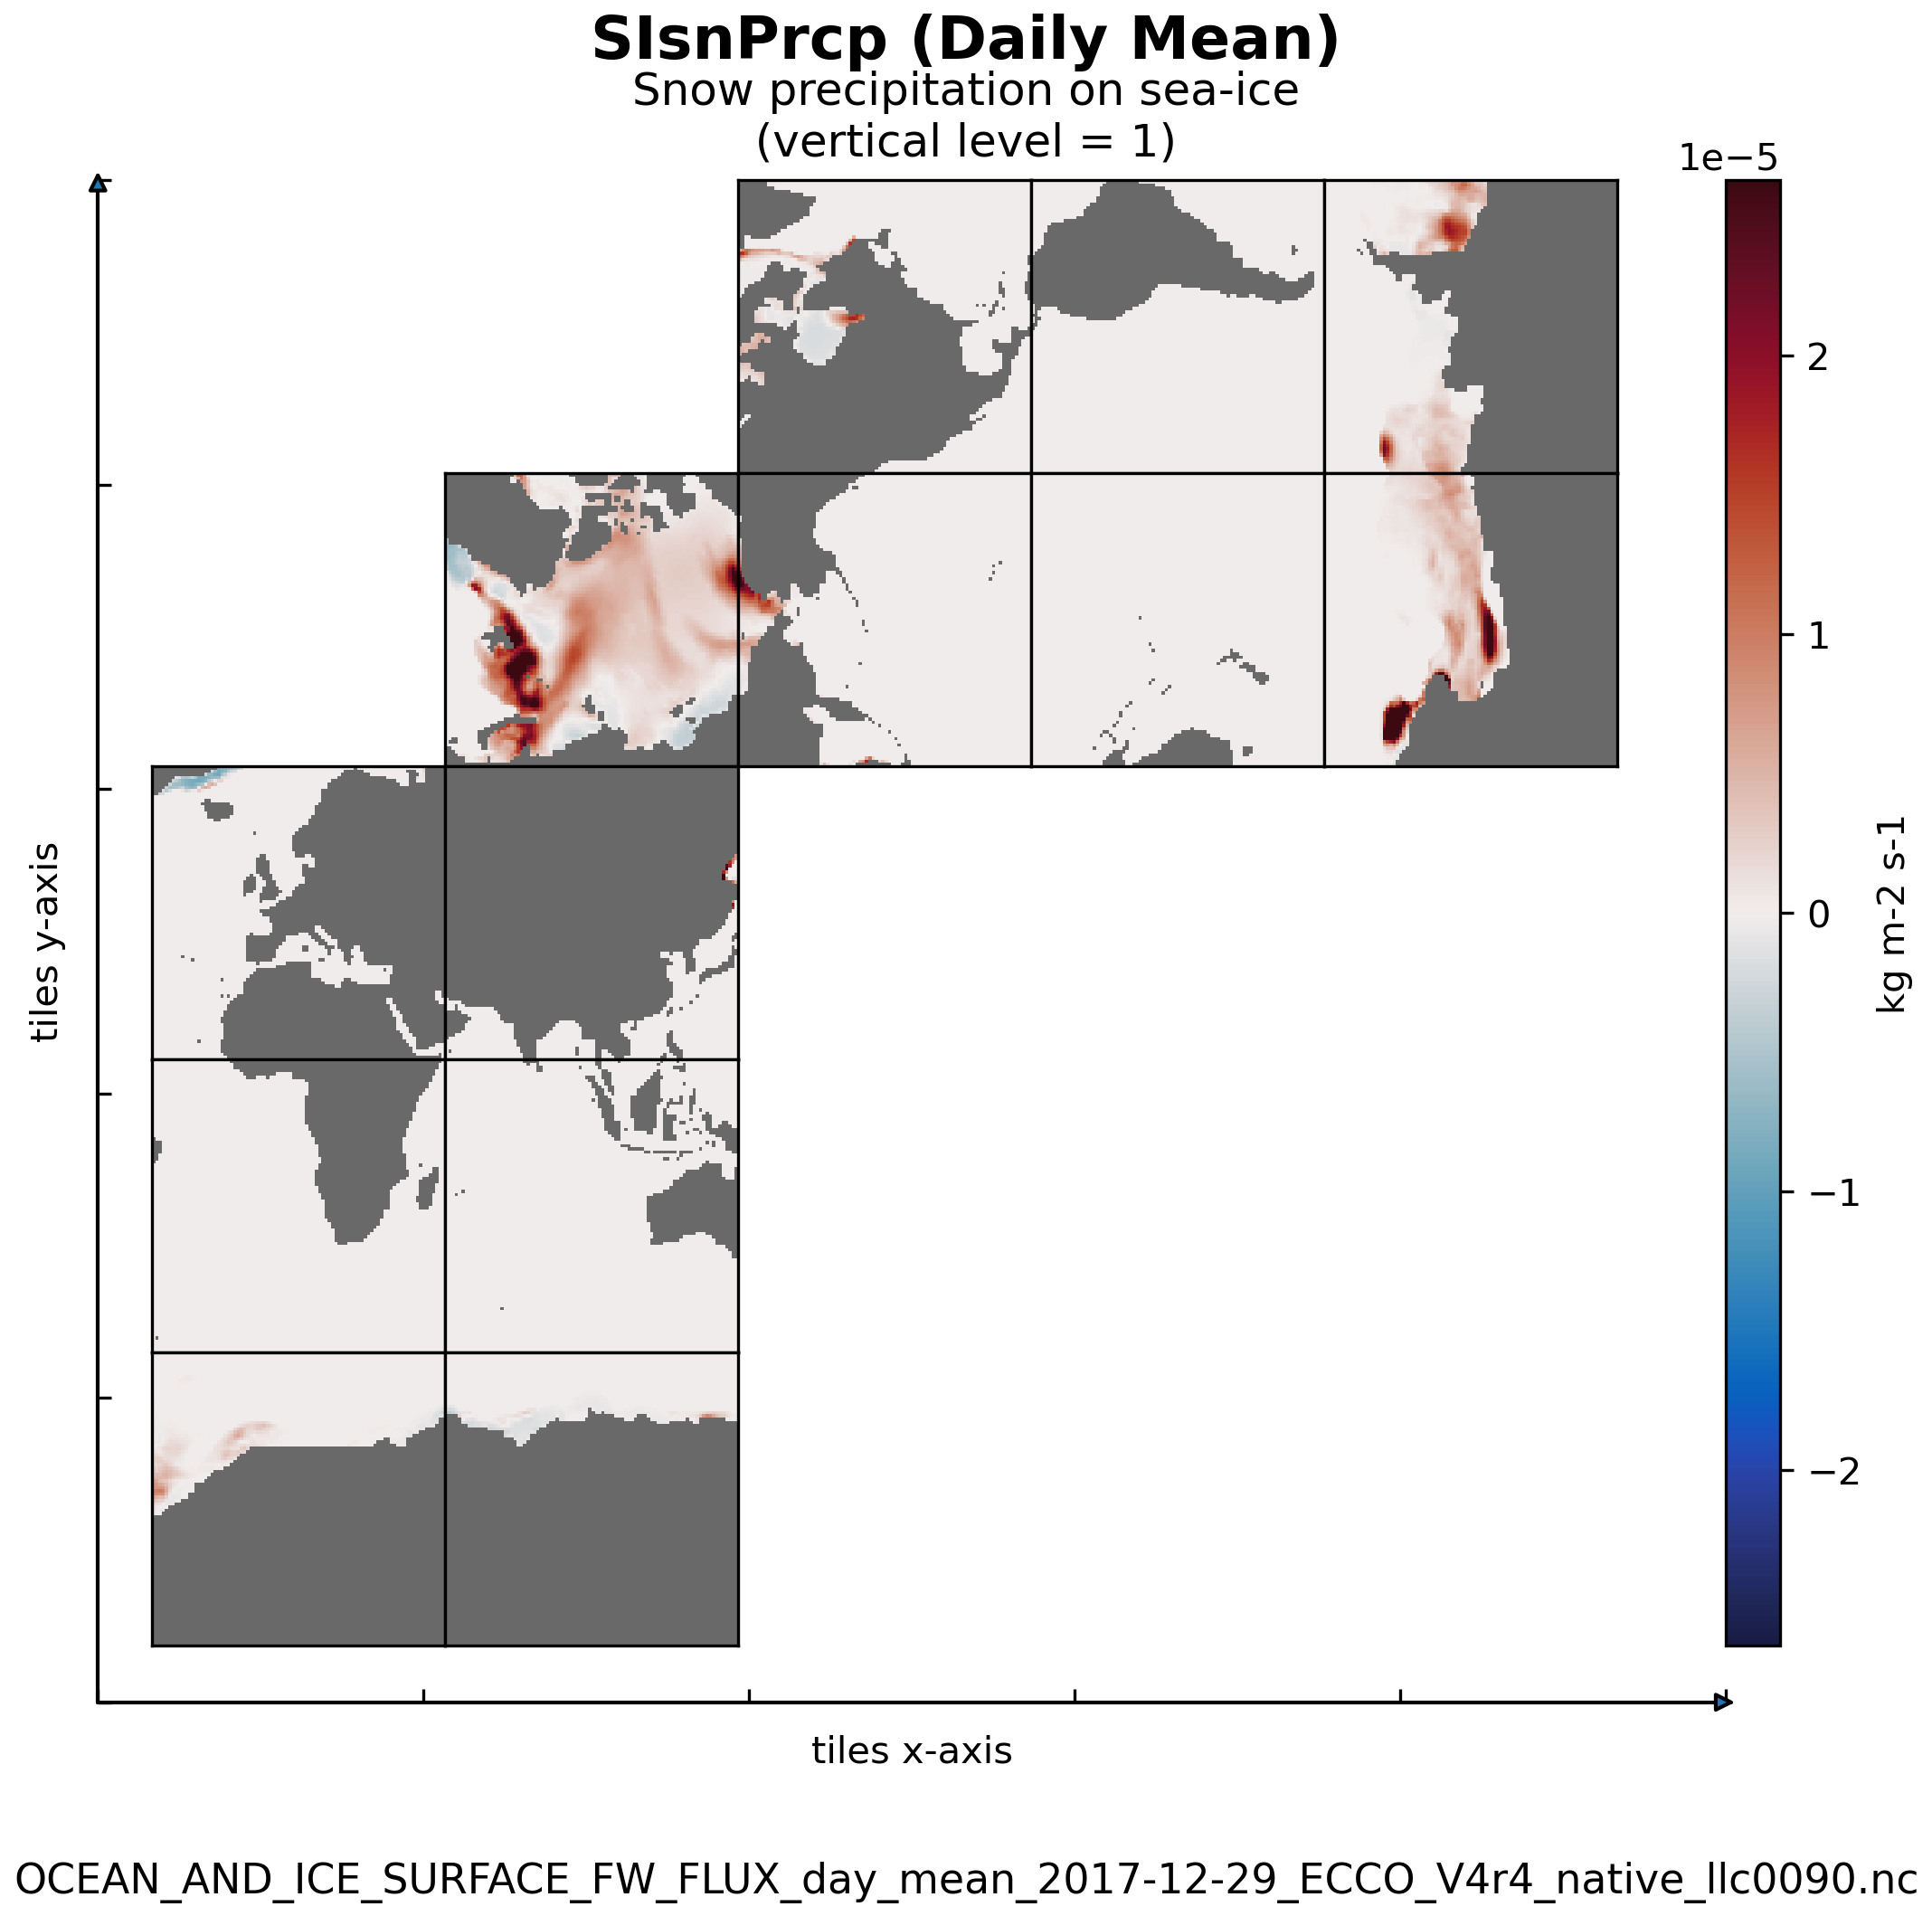
\includegraphics[scale=0.5]{../images/plots/native_plots/Ocean_and_Sea-Ice_Surface_Freshwater_Fluxes/SIsnPrcp.png}
\caption{\\Dataset: OCEAN\_AND\_ICE\_SURFACE\_FW\_FLUX\\Variable: SIsnPrcp}
\label{tab:table-OCEAN_AND_ICE_SURFACE_FW_FLUX_SIsnPrcp-Plot}
\end{figure}
\pagebreak
\subsubsection{Native Variable oceFWflx}
\begin{longtable}{|p{0.06\textwidth}|p{0.41\textwidth}|p{0.39\textwidth}|p{0.06\textwidth}|}
\caption{CDL description of OCEAN\_AND\_ICE\_SURFACE\_FW\_FLUX's oceFWflx variable}
\label{tab:table-OCEAN_AND_ICE_SURFACE_FW_FLUX_oceFWflx} \\ 
\hline \endhead \hline \endfoot
\rowcolor{lightgray} \textbf{Storage Type} & \textbf{Variable Name} & \textbf{Description} & \textbf{Unit} \\ \hline
float32 & oceFWflx & Net freshwater flux into the ocean & kg m-2 s-1 \\ \hline
\rowcolor{lightgray}  \multicolumn{4}{|p{1.00\textwidth}|}{\textbf{CDL Description}} \\ \hline
\multicolumn{4}{|p{1.00\textwidth}|}{\makecell{\parbox{1\textwidth}{float32 oceFWflx(time, tile, j, i)\\
\hspace*{0.5cm}oceFWflx: \_FillValue = 9.96921e+36\\
\hspace*{0.5cm}oceFWflx: long\_name = Net freshwater flux into the ocean\\
\hspace*{0.5cm}oceFWflx: units = kg m: 2 s: 1\\
\hspace*{0.5cm}oceFWflx: coverage\_content\_type = modelResult\\
\hspace*{0.5cm}oceFWflx: direction = >0 decreases salinity (SALT)\\
\hspace*{0.5cm}oceFWflx: standard\_name = water\_flux\_into\_sea\_water\\
\hspace*{0.5cm}oceFWflx: coordinates = YC XC time\\
\hspace*{0.5cm}oceFWflx: valid\_min = : 0.003914969973266125\\
\hspace*{0.5cm}oceFWflx: valid\_max = 0.008299433626234531}}} \\ \hline
\rowcolor{lightgray} \multicolumn{4}{|p{1.00\textwidth}|}{\textbf{Comments}} \\ \hline
\multicolumn{4}{|p{1\textwidth}|}{Net freshwater flux into the ocean including contributions from runoff, evaporation, precipitation, and mass exchange with sea-ice due to melting and freezing and snow melting. Note: oceFWflx does NOT include freshwater fluxes between the atmosphere and sea-ice and snow. The variable 'SIatmFW' accounts for freshwater fluxes out of the combined ocean+sea-ice+snow reservoir.} \\ \hline
\end{longtable}

\begin{figure}[H]
\centering
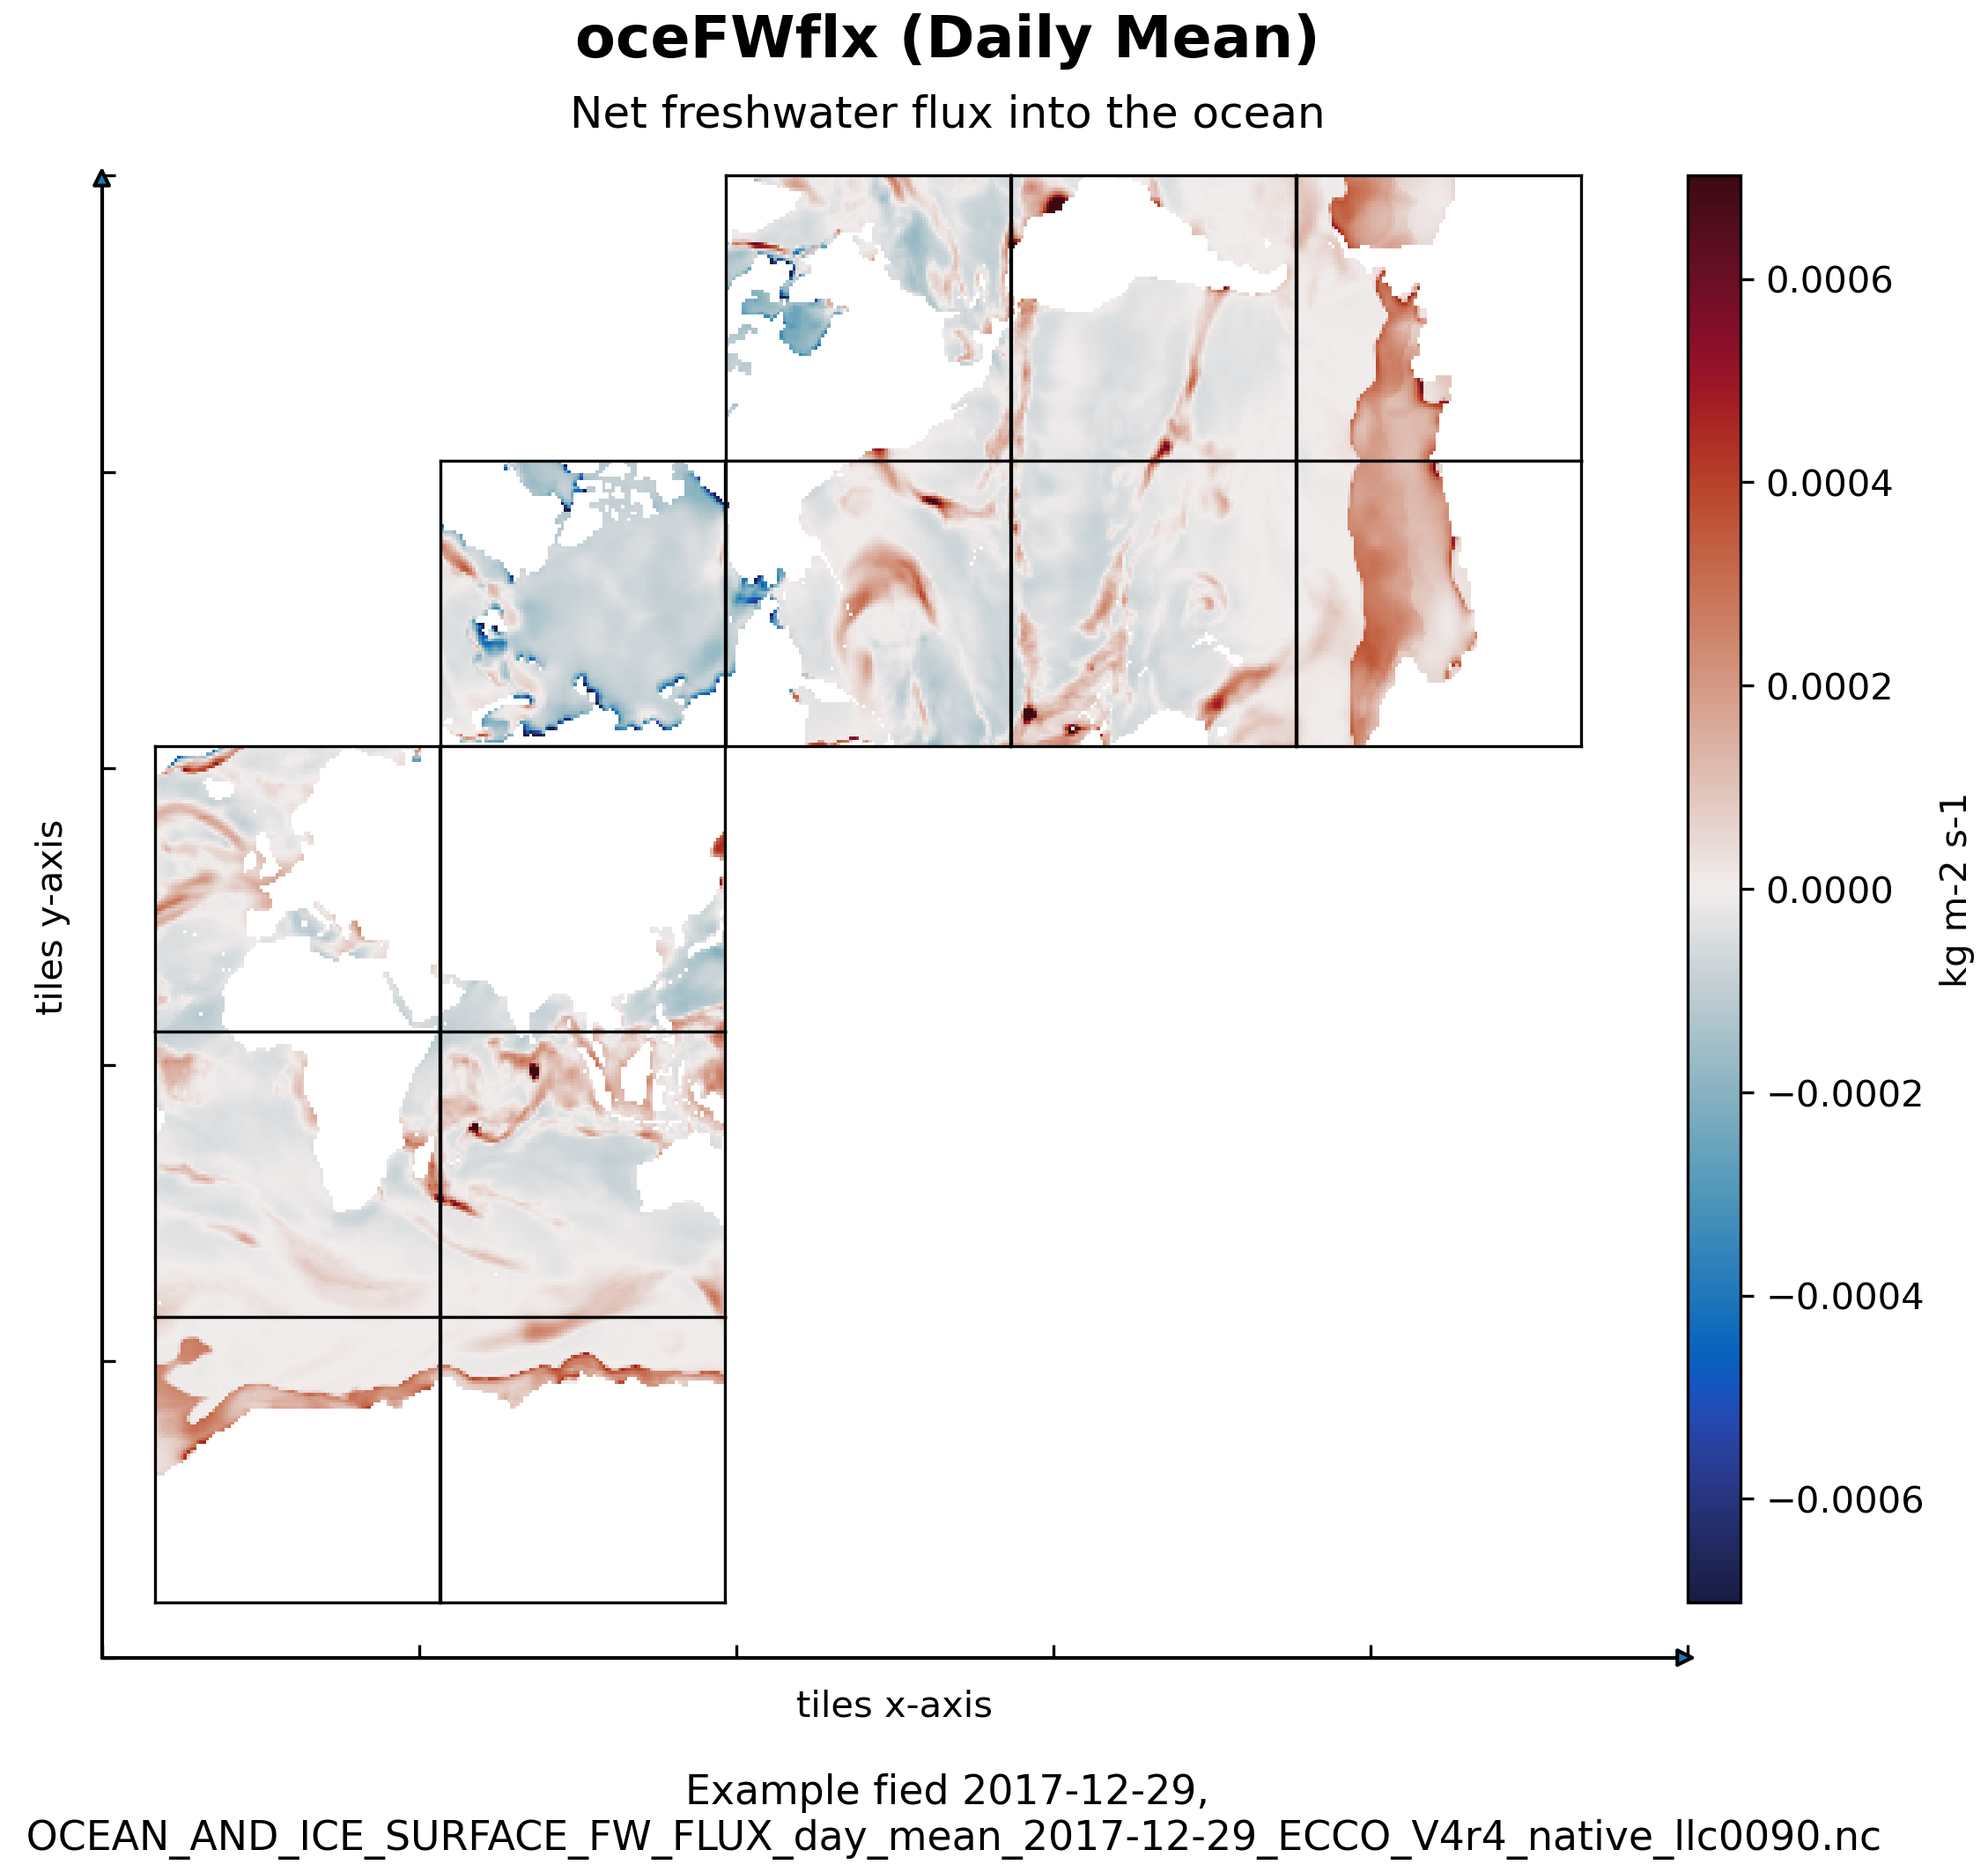
\includegraphics[scale=0.5]{../images/plots/native_plots/Ocean_and_Sea-Ice_Surface_Freshwater_Fluxes/oceFWflx.png}
\caption{\\Dataset: OCEAN\_AND\_ICE\_SURFACE\_FW\_FLUX\\Variable: oceFWflx}
\label{tab:table-OCEAN_AND_ICE_SURFACE_FW_FLUX_oceFWflx-Plot}
\end{figure}
\pagebreak
\subsection{Native NetCDF OCEAN\_AND\_ICE\_SURFACE\_HEAT\_FLUX}
\newp
\begin{longtable}{|p{0.1\textwidth}|p{0.5\textwidth}|}
\caption{Variables in the dataset OCEAN\_AND\_ICE\_SURFACE\_HEAT\_FLUX}
\label{tab:table-OCEAN_AND_ICE_SURFACE_HEAT_FLUX-fields} \\ 
\hline \endhead \hline \endfoot
\rowcolor{lightgray} \textbf{Dataset:} & \textbf{OCEAN\_AND\_ICE\_SURFACE\_HEAT\_FLUX} \\ \hline
Field: &EXFhl \\ \hline
Field: &EXFhs \\ \hline
Field: &EXFlwdn \\ \hline
Field: &EXFswdn \\ \hline
Field: &EXFqnet \\ \hline
Field: &oceQnet \\ \hline
Field: &SIatmQnt \\ \hline
Field: &TFLUX \\ \hline
Field: &EXFswnet \\ \hline
Field: &EXFlwnet \\ \hline
Field: &oceQsw \\ \hline
Field: &SIaaflux \\ \hline
\end{longtable}

\pagebreak
\subsubsection{Native Variable EXFhl}
\begin{longtable}{|p{0.06\textwidth}|p{0.41\textwidth}|p{0.39\textwidth}|p{0.06\textwidth}|}
\caption{CDL description of OCEAN\_AND\_ICE\_SURFACE\_HEAT\_FLUX's EXFhl variable}
\label{tab:table-OCEAN_AND_ICE_SURFACE_HEAT_FLUX_EXFhl} \\ 
\hline \endhead \hline \endfoot
\rowcolor{lightgray} \textbf{Storage Type} & \textbf{Variable Name} & \textbf{Description} & \textbf{Unit} \\ \hline
float32 & EXFhl & Open ocean air-sea latent heat flux & W m-2 \\ \hline
\rowcolor{lightgray}  \multicolumn{4}{|p{1.00\textwidth}|}{\textbf{CDL Description}} \\ \hline
\multicolumn{4}{|p{1.00\textwidth}|}{\makecell{\parbox{1\textwidth}{float32 EXFhl(time, tile, j, i)\\
\hspace*{0.5cm}EXFhl: \_FillValue = 9.96921e+36\\
\hspace*{0.5cm}EXFhl: long\_name = Open ocean air: sea latent heat flux\\
\hspace*{0.5cm}EXFhl: units = W m: 2\\
\hspace*{0.5cm}EXFhl: coverage\_content\_type = modelResult\\
\hspace*{0.5cm}EXFhl: direction = >0 increases potential temperature (THETA)\\
\hspace*{0.5cm}EXFhl: standard\_name = surface\_downward\_latent\_heat\_flux\\
\hspace*{0.5cm}EXFhl: coordinates = XC time YC\\
\hspace*{0.5cm}EXFhl: valid\_min = : 1772.513671875\\
\hspace*{0.5cm}EXFhl: valid\_max = 273.9528503417969}}} \\ \hline
\rowcolor{lightgray} \multicolumn{4}{|p{1.00\textwidth}|}{\textbf{Comments}} \\ \hline
\multicolumn{4}{|p{1\textwidth}|}{Air-sea latent heat flux per unit area of open water (not covered by sea-ice). Note: calculated from the bulk formula following Large and Yeager (2004) NCAR/TN-460+STR.} \\ \hline
\end{longtable}

\begin{figure}[H]
\centering
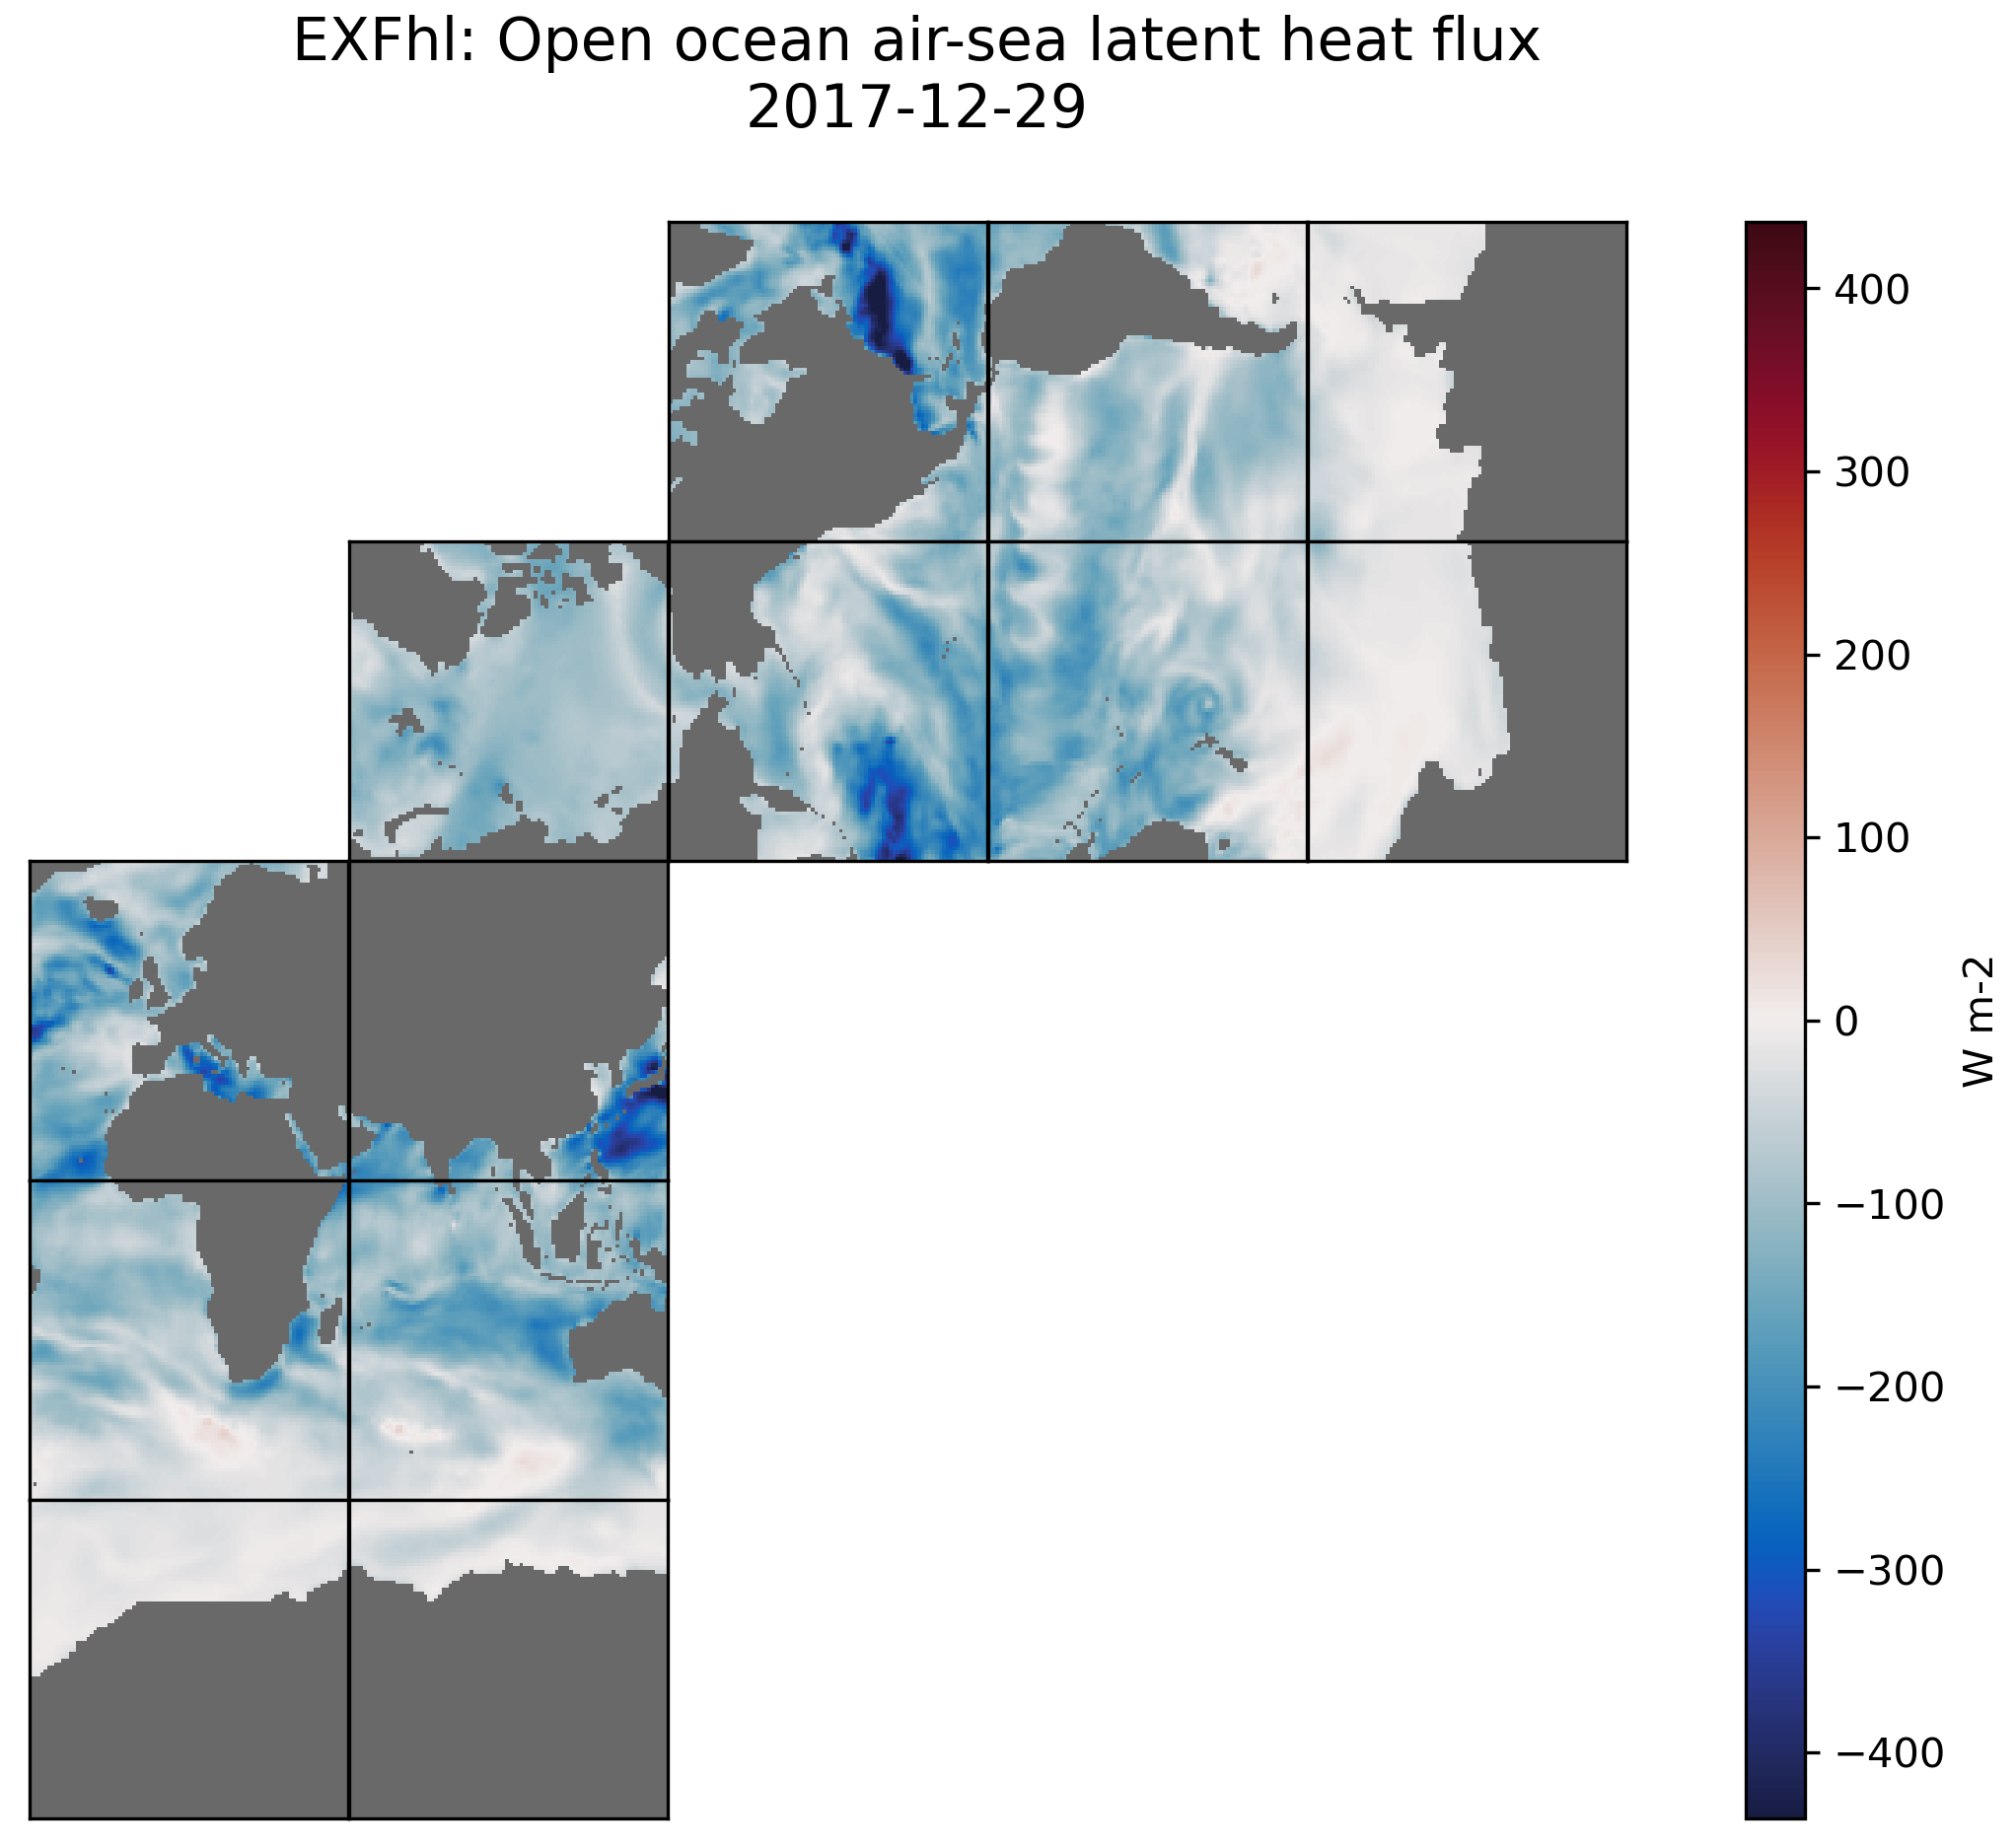
\includegraphics[scale=0.5]{../images/plots/native_plots/Ocean_and_Sea-Ice_Surface_Heat_Fluxes/EXFhl.png}
\caption{\\Dataset: OCEAN\_AND\_ICE\_SURFACE\_HEAT\_FLUX\\Variable: EXFhl}
\label{tab:table-OCEAN_AND_ICE_SURFACE_HEAT_FLUX_EXFhl-Plot}
\end{figure}
\pagebreak
\subsubsection{Native Variable EXFhs}
\begin{longtable}{|p{0.06\textwidth}|p{0.41\textwidth}|p{0.39\textwidth}|p{0.06\textwidth}|}
\caption{CDL description of OCEAN\_AND\_ICE\_SURFACE\_HEAT\_FLUX's EXFhs variable}
\label{tab:table-OCEAN_AND_ICE_SURFACE_HEAT_FLUX_EXFhs} \\ 
\hline \endhead \hline \endfoot
\rowcolor{lightgray} \textbf{Storage Type} & \textbf{Variable Name} & \textbf{Description} & \textbf{Unit} \\ \hline
float32 & EXFhs & Open ocean air-sea sensible heat flux & W m-2 \\ \hline
\rowcolor{lightgray}  \multicolumn{4}{|p{1.00\textwidth}|}{\textbf{CDL Description}} \\ \hline
\multicolumn{4}{|p{1.00\textwidth}|}{\makecell{\parbox{1\textwidth}{float32 EXFhs(time, tile, j, i)\\
\hspace*{0.5cm}EXFhs: \_FillValue = 9.96921e+36\\
\hspace*{0.5cm}EXFhs: long\_name = Open ocean air: sea sensible heat flux\\
\hspace*{0.5cm}EXFhs: units = W m: 2\\
\hspace*{0.5cm}EXFhs: coverage\_content\_type = modelResult\\
\hspace*{0.5cm}EXFhs: direction = >0 increases potential temperature (THETA)\\
\hspace*{0.5cm}EXFhs: standard\_name = surface\_downward\_sensible\_heat\_flux\\
\hspace*{0.5cm}EXFhs: coordinates = XC time YC\\
\hspace*{0.5cm}EXFhs: valid\_min = : 2478.766357421875\\
\hspace*{0.5cm}EXFhs: valid\_max = 362.8300476074219}}} \\ \hline
\rowcolor{lightgray} \multicolumn{4}{|p{1.00\textwidth}|}{\textbf{Comments}} \\ \hline
\multicolumn{4}{|p{1\textwidth}|}{Air-sea sensible heat flux per unit area of open water (not covered by sea-ice). Note: calculated from the bulk formula following Large and Yeager (2004) NCAR/TN-460+STR.} \\ \hline
\end{longtable}

\begin{figure}[H]
\centering
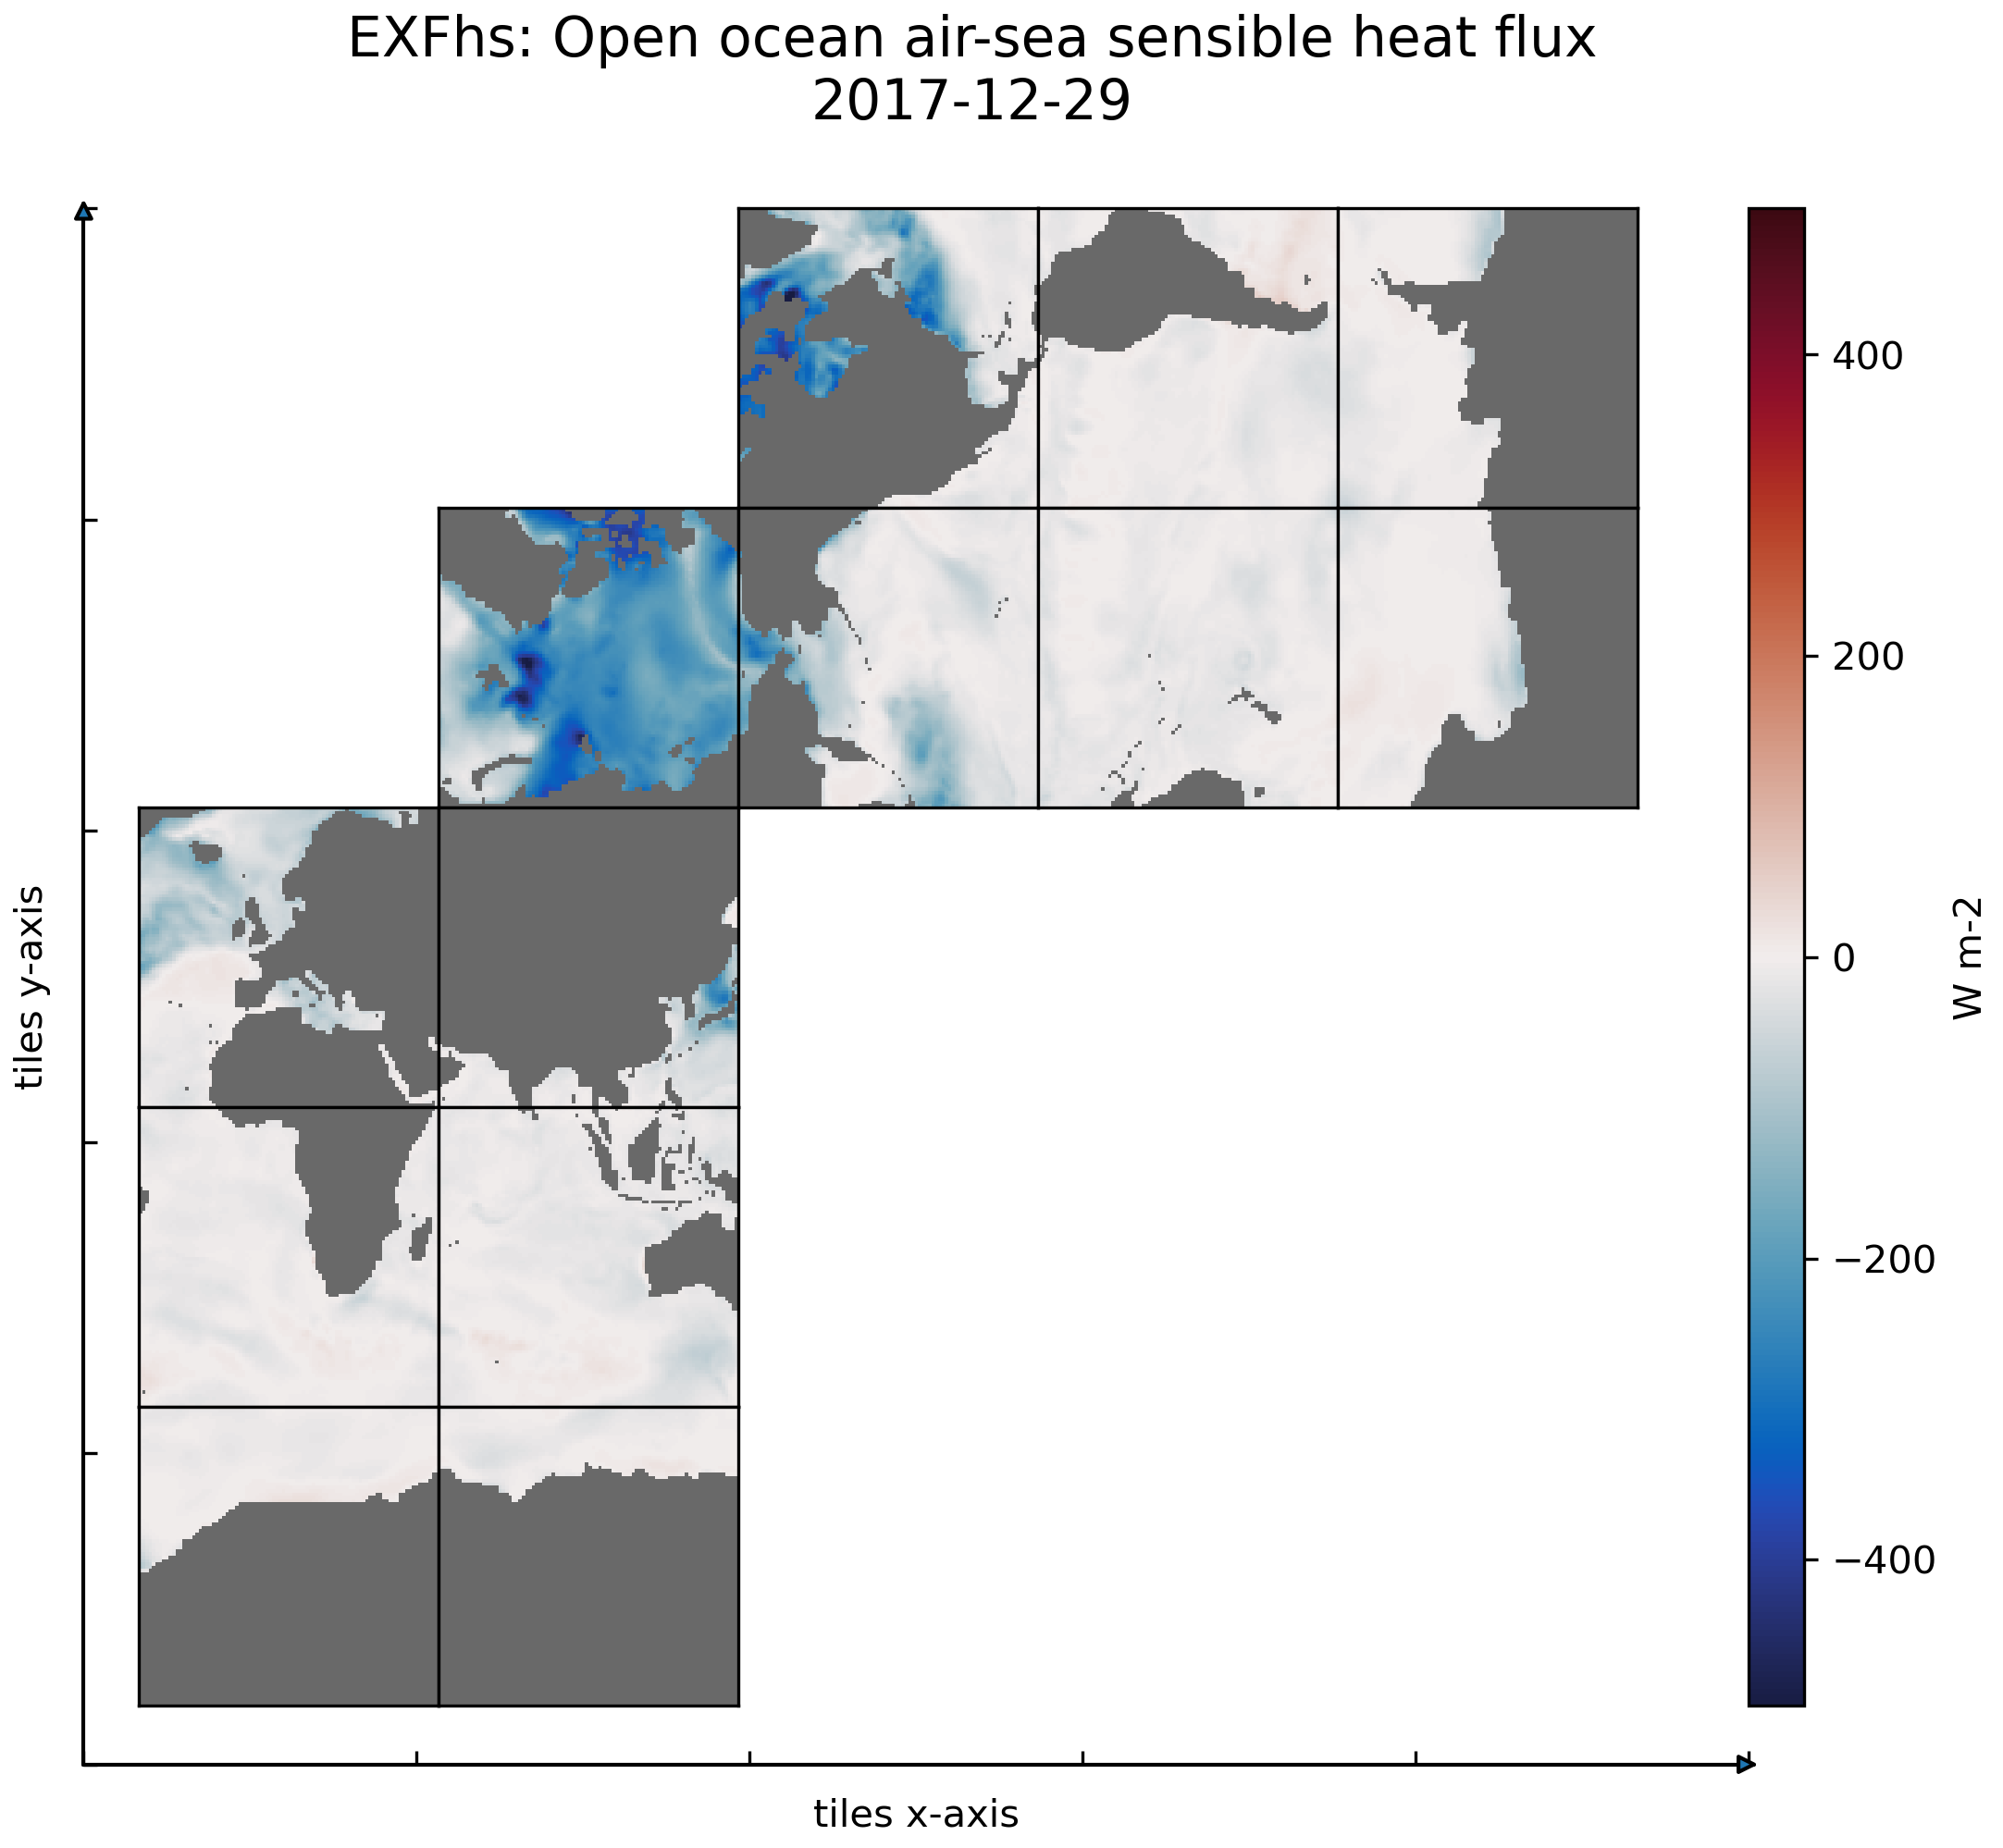
\includegraphics[scale=0.5]{../images/plots/native_plots/Ocean_and_Sea-Ice_Surface_Heat_Fluxes/EXFhs.png}
\caption{\\Dataset: OCEAN\_AND\_ICE\_SURFACE\_HEAT\_FLUX\\Variable: EXFhs}
\label{tab:table-OCEAN_AND_ICE_SURFACE_HEAT_FLUX_EXFhs-Plot}
\end{figure}
\pagebreak
\subsubsection{Native Variable EXFlwdn}
\begin{longtable}{|p{0.06\textwidth}|p{0.41\textwidth}|p{0.39\textwidth}|p{0.06\textwidth}|}
\caption{CDL description of OCEAN\_AND\_ICE\_SURFACE\_HEAT\_FLUX's EXFlwdn variable}
\label{tab:table-OCEAN_AND_ICE_SURFACE_HEAT_FLUX_EXFlwdn} \\ 
\hline \endhead \hline \endfoot
\rowcolor{lightgray} \textbf{Storage Type} & \textbf{Variable Name} & \textbf{Description} & \textbf{Unit} \\ \hline
float32 & EXFlwdn & Downward longwave radiative flux & W m-2 \\ \hline
\rowcolor{lightgray}  \multicolumn{4}{|p{1.00\textwidth}|}{\textbf{CDL Description}} \\ \hline
\multicolumn{4}{|p{1.00\textwidth}|}{\makecell{\parbox{1\textwidth}{float32 EXFlwdn(time, tile, j, i)\\
\hspace*{0.5cm}EXFlwdn: \_FillValue = 9.96921e+36\\
\hspace*{0.5cm}EXFlwdn: long\_name = Downward longwave radiative flux\\
\hspace*{0.5cm}EXFlwdn: units = W m: 2\\
\hspace*{0.5cm}EXFlwdn: coverage\_content\_type = modelResult\\
\hspace*{0.5cm}EXFlwdn: direction = >0 increases potential temperature (THETA)\\
\hspace*{0.5cm}EXFlwdn: standard\_name = surface\_downwelling\_longwave\_flux\_in\_air\\
\hspace*{0.5cm}EXFlwdn: coordinates = XC time YC\\
\hspace*{0.5cm}EXFlwdn: valid\_min = 4.188045501708984\\
\hspace*{0.5cm}EXFlwdn: valid\_max = 513.3919067382812}}} \\ \hline
\rowcolor{lightgray} \multicolumn{4}{|p{1.00\textwidth}|}{\textbf{Comments}} \\ \hline
\multicolumn{4}{|p{1\textwidth}|}{Downward longwave radiative flux. Note: sum of ERA-Interim downward longwave radiation and the control adjustment from ocean state estimation.} \\ \hline
\end{longtable}

\begin{figure}[H]
\centering
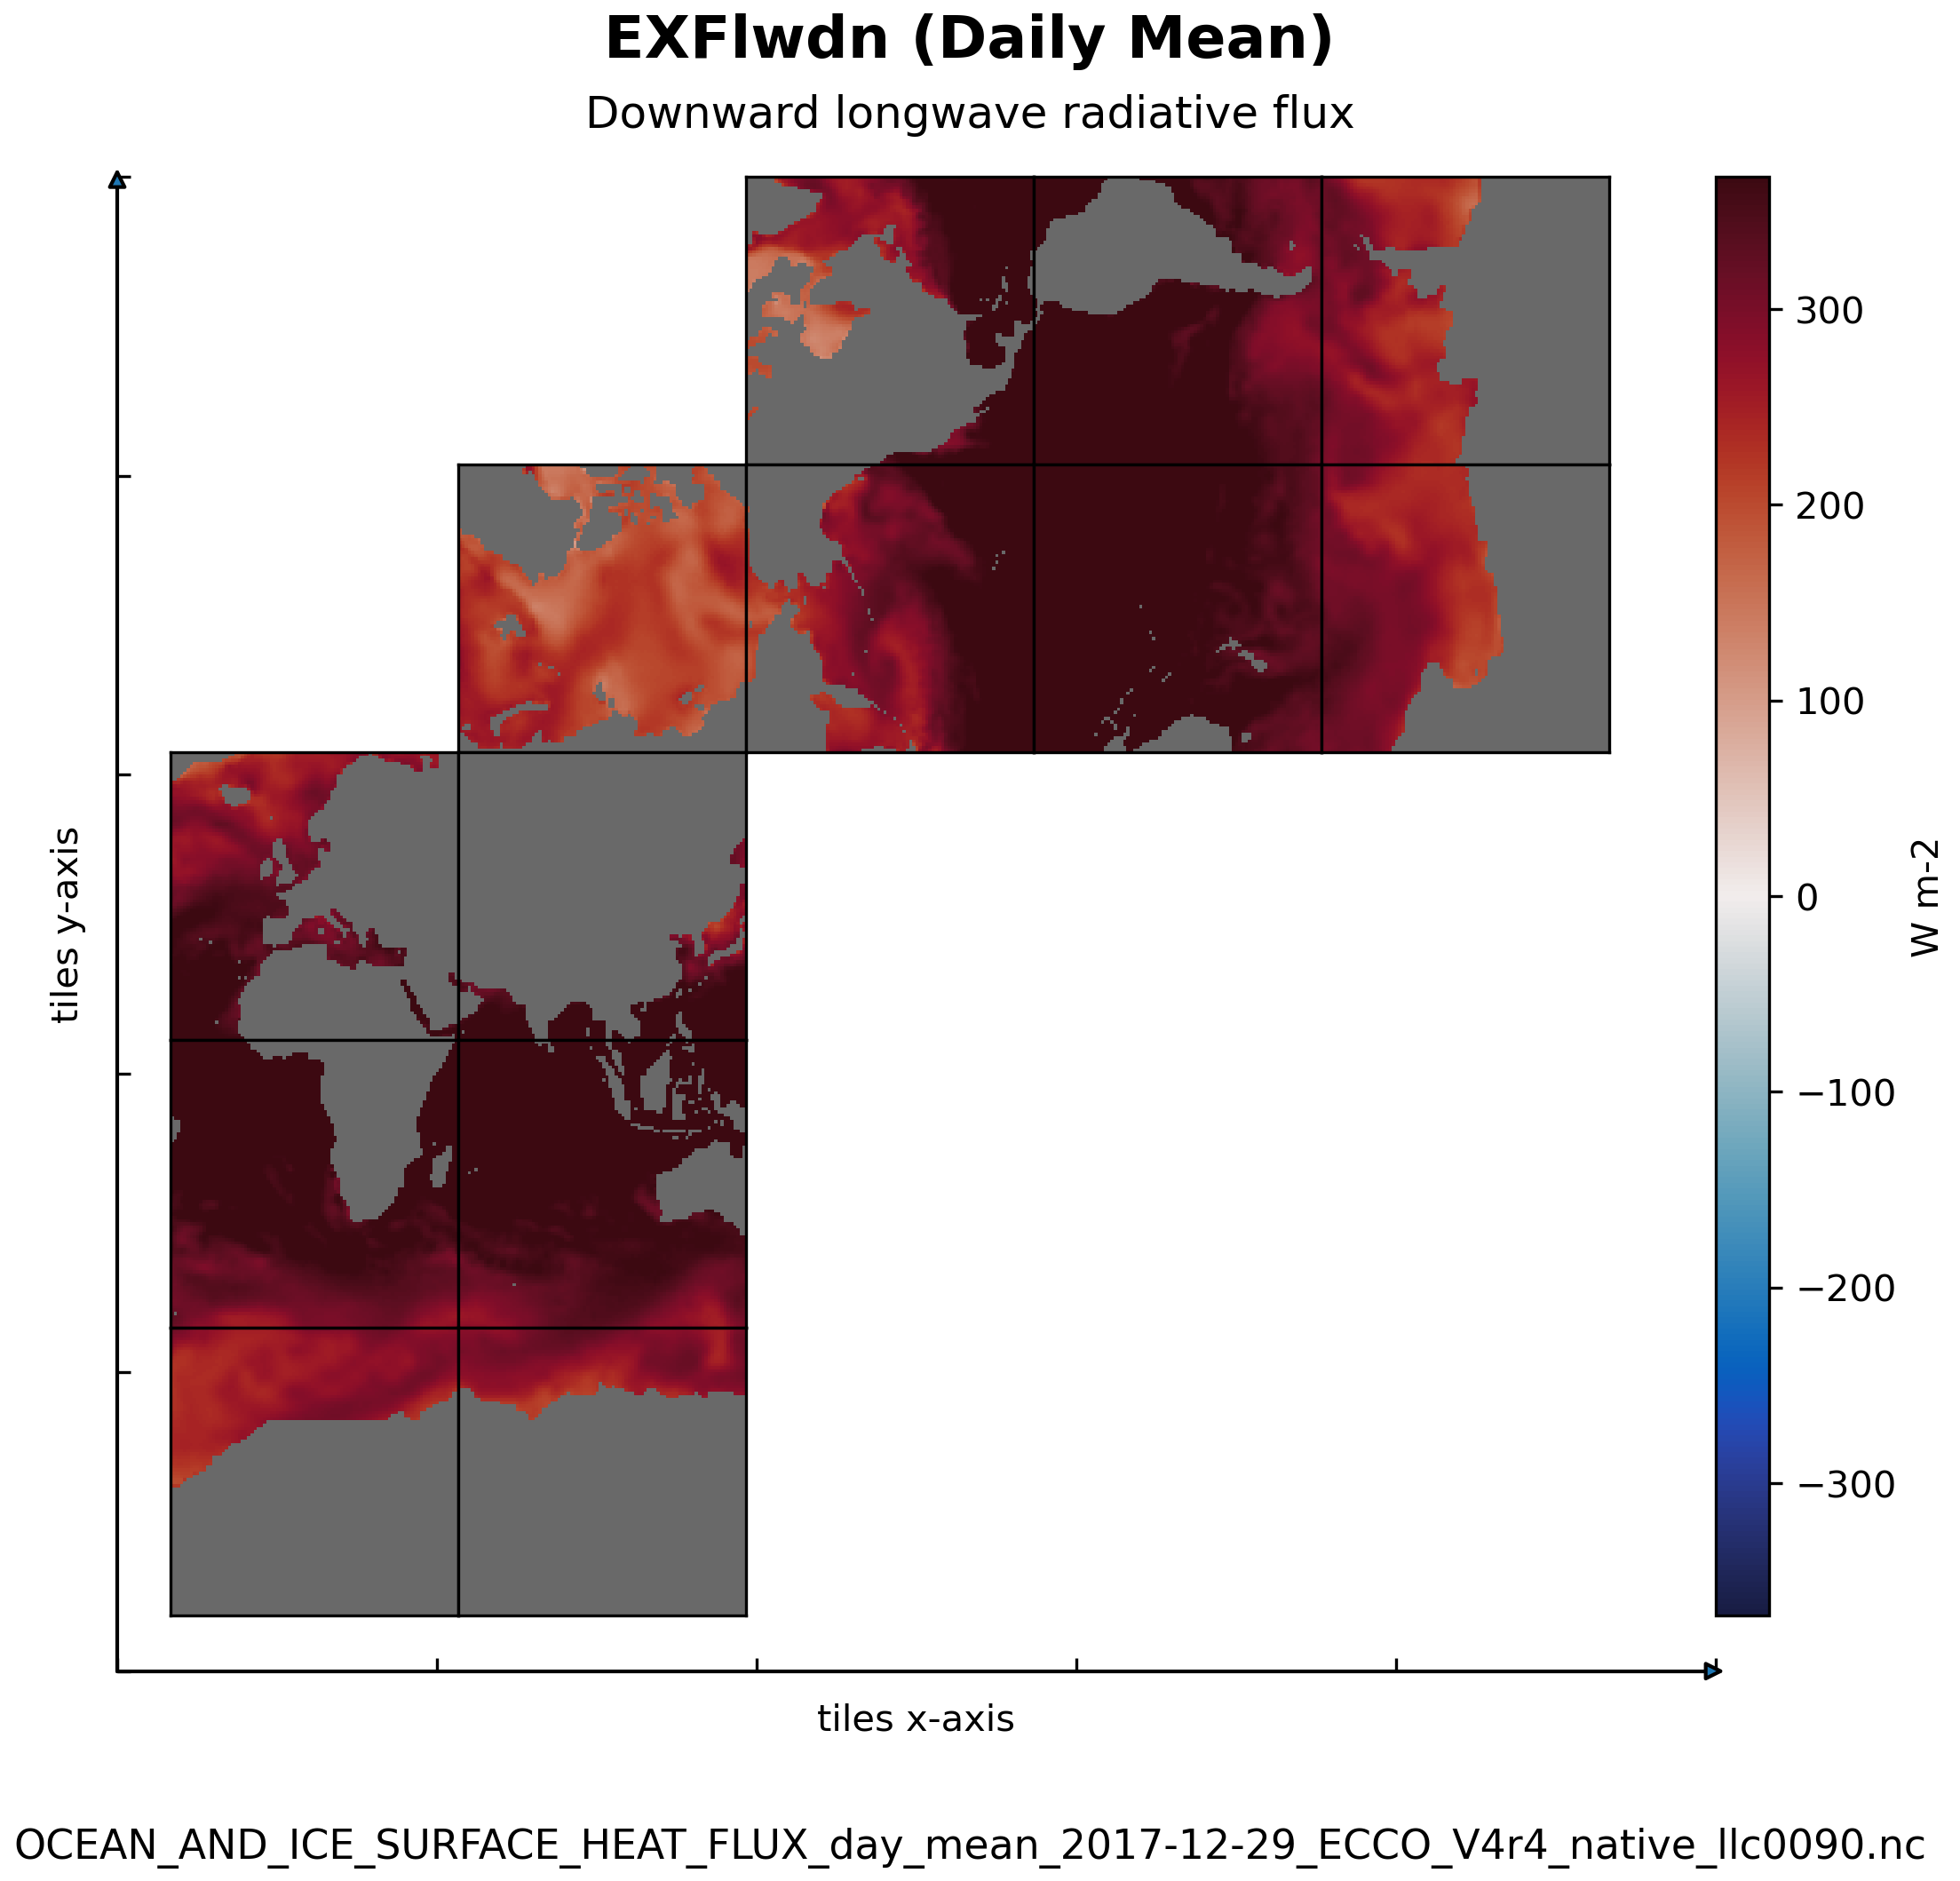
\includegraphics[scale=0.5]{../images/plots/native_plots/Ocean_and_Sea-Ice_Surface_Heat_Fluxes/EXFlwdn.png}
\caption{\\Dataset: OCEAN\_AND\_ICE\_SURFACE\_HEAT\_FLUX\\Variable: EXFlwdn}
\label{tab:table-OCEAN_AND_ICE_SURFACE_HEAT_FLUX_EXFlwdn-Plot}
\end{figure}
\pagebreak
\subsubsection{Native Variable EXFlwnet}
\begin{longtable}{|p{0.06\textwidth}|p{0.41\textwidth}|p{0.39\textwidth}|p{0.06\textwidth}|}
\caption{CDL description of OCEAN\_AND\_ICE\_SURFACE\_HEAT\_FLUX's EXFlwnet variable}
\label{tab:table-OCEAN_AND_ICE_SURFACE_HEAT_FLUX_EXFlwnet} \\ 
\hline \endhead \hline \endfoot
\rowcolor{lightgray} \textbf{Storage Type} & \textbf{Variable Name} & \textbf{Description} & \textbf{Unit} \\ \hline
float32 & EXFlwnet & Net open ocean longwave radiative flux & W m-2 \\ \hline
\rowcolor{lightgray}  \multicolumn{4}{|p{1.00\textwidth}|}{\textbf{CDL Description}} \\ \hline
\multicolumn{4}{|p{1.00\textwidth}|}{\makecell{\parbox{1\textwidth}{float32 EXFlwnet(time, tile, j, i)\\
\hspace*{0.5cm}EXFlwnet: \_FillValue = 9.96921e+36\\
\hspace*{0.5cm}EXFlwnet: long\_name = Net open ocean longwave radiative flux\\
\hspace*{0.5cm}EXFlwnet: units = W m: 2\\
\hspace*{0.5cm}EXFlwnet: coverage\_content\_type = modelResult\\
\hspace*{0.5cm}EXFlwnet: direction = >0 increases potential temperature (THETA)\\
\hspace*{0.5cm}EXFlwnet: standard\_name = surface\_net\_downward\_longwave\_flux\\
\hspace*{0.5cm}EXFlwnet: coordinates = XC time YC\\
\hspace*{0.5cm}EXFlwnet: valid\_min = : 144.3661346435547\\
\hspace*{0.5cm}EXFlwnet: valid\_max = 293.4114990234375}}} \\ \hline
\rowcolor{lightgray} \multicolumn{4}{|p{1.00\textwidth}|}{\textbf{Comments}} \\ \hline
\multicolumn{4}{|p{1\textwidth}|}{Net longwave radiative flux per unit area of open water (not covered by sea-ice). Note: net longwave radiation over open water calculated from downward longwave radiation (EXFlwdn) and upward longwave radiation from ocean and sea-ice thermal emission (Stefan-Boltzman law).} \\ \hline
\end{longtable}

\begin{figure}[H]
\centering
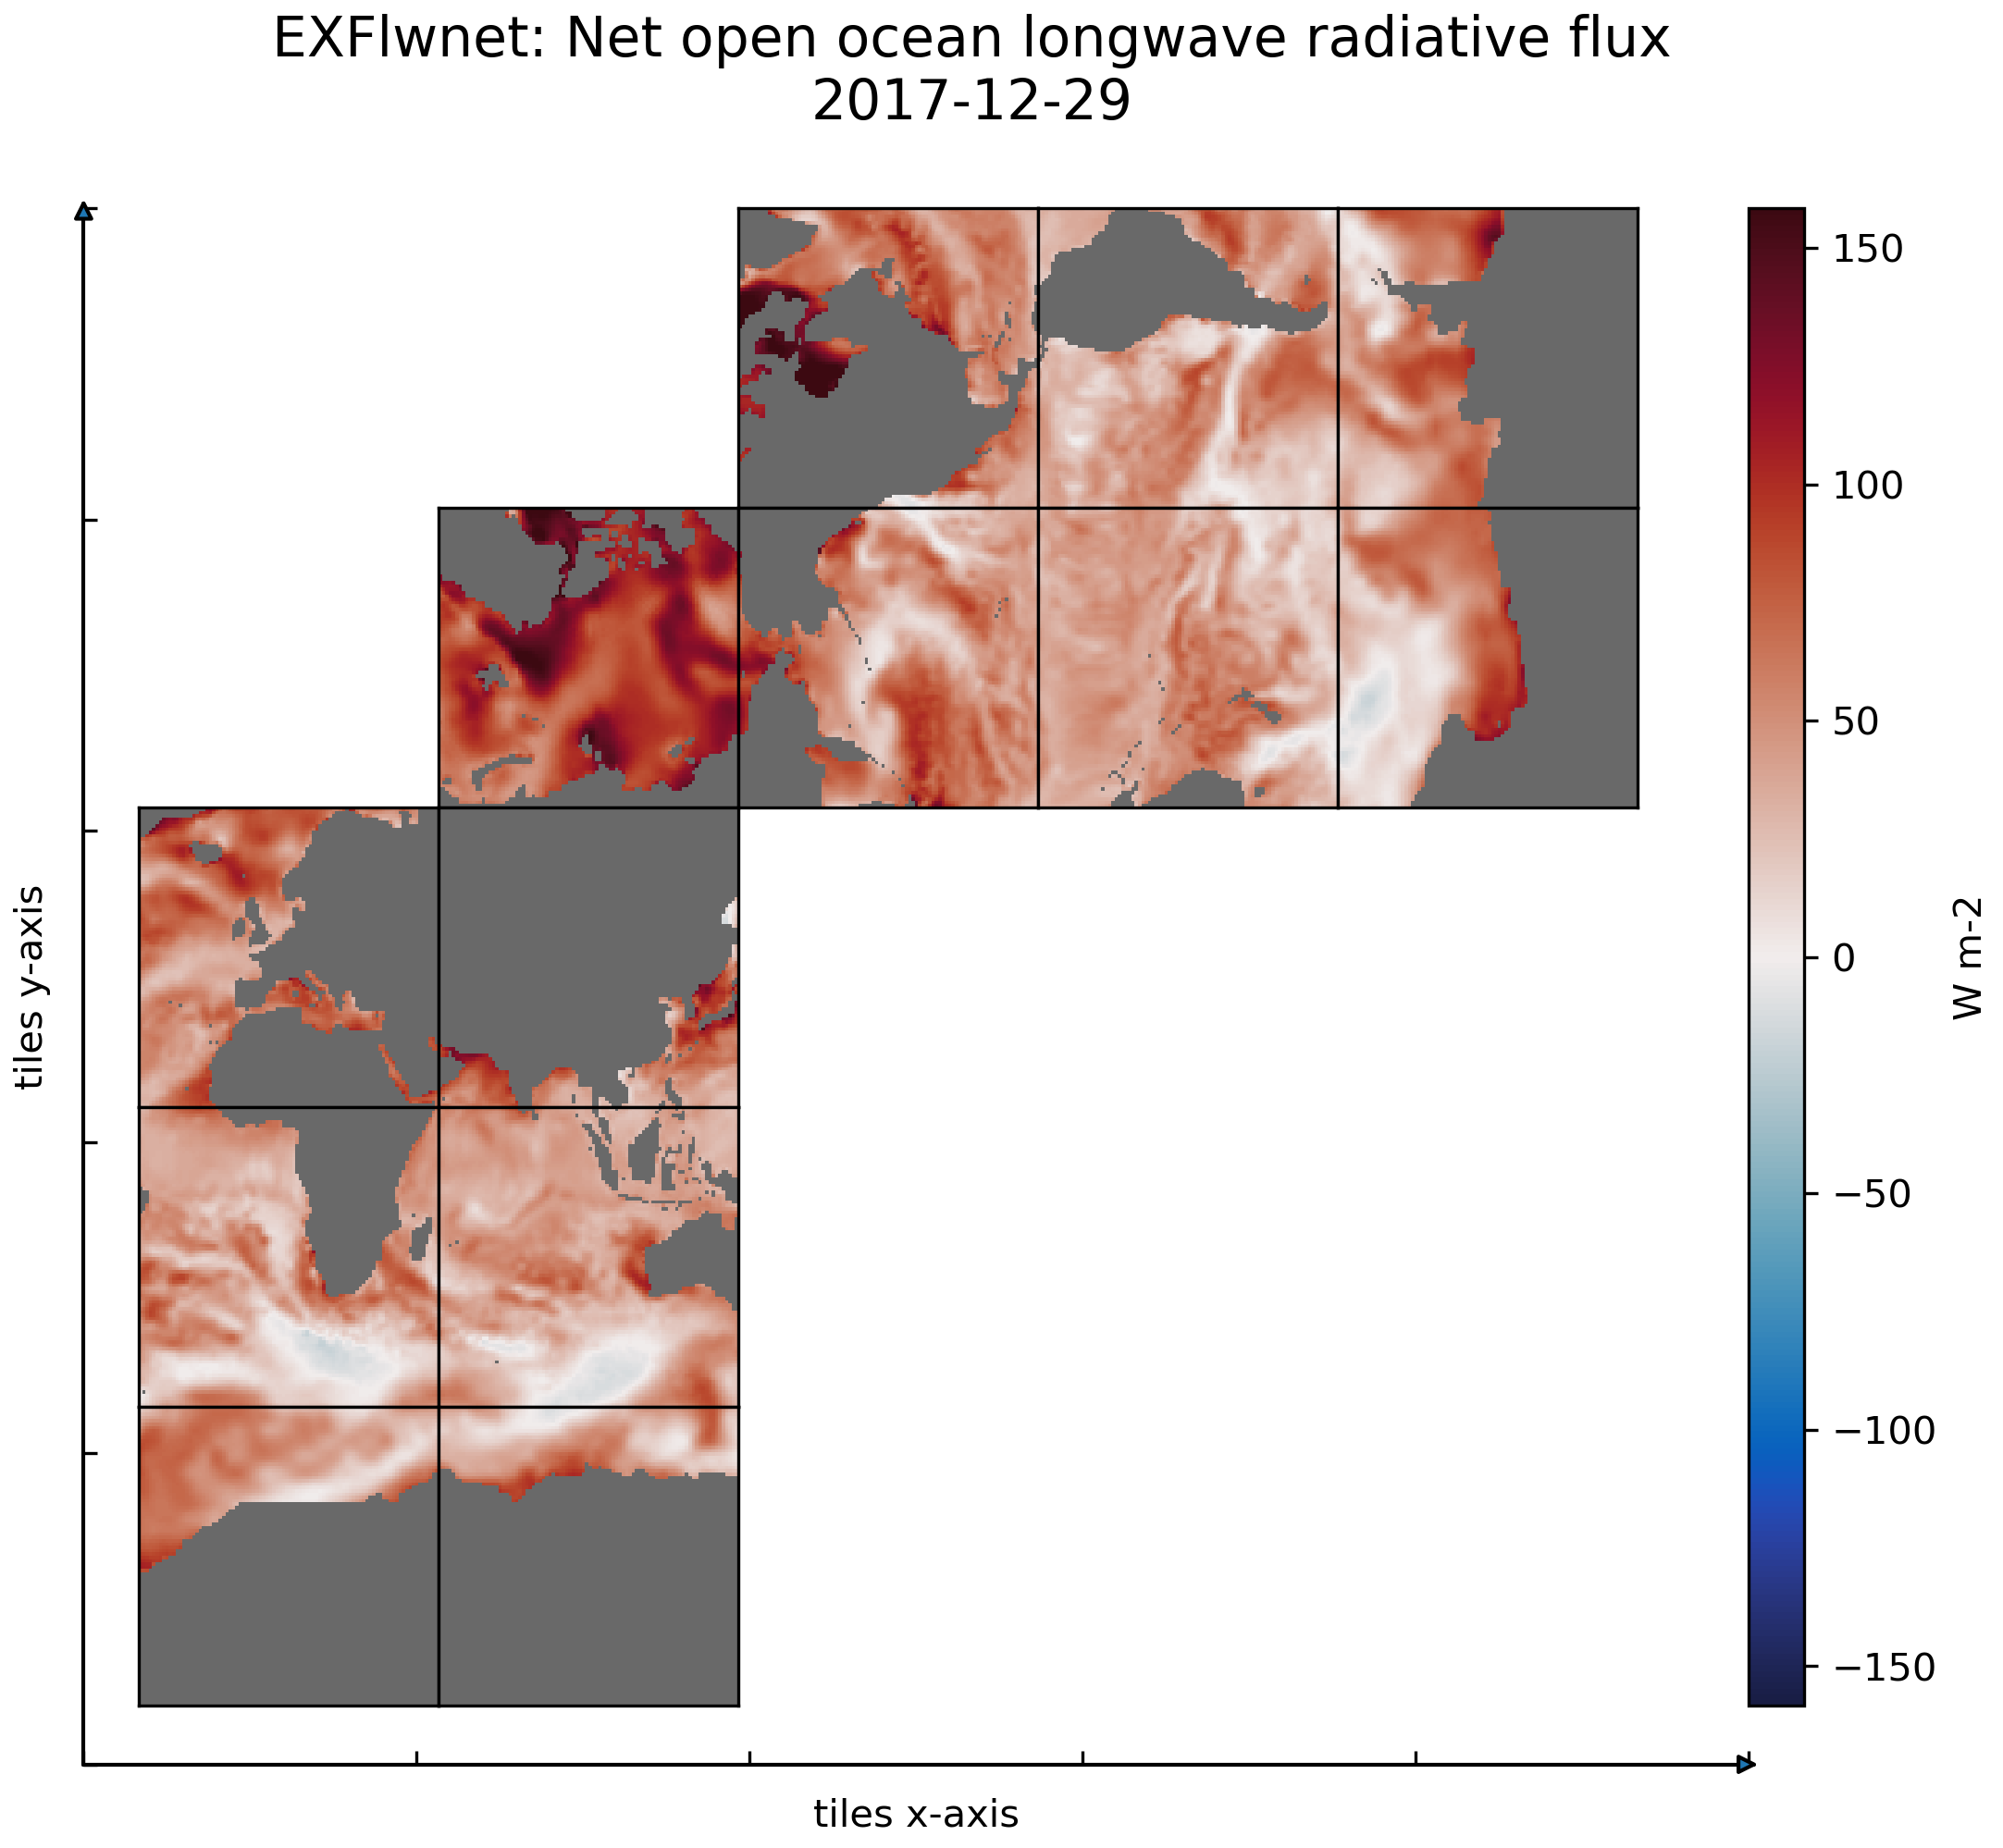
\includegraphics[scale=0.5]{../images/plots/native_plots/Ocean_and_Sea-Ice_Surface_Heat_Fluxes/EXFlwnet.png}
\caption{\\Dataset: OCEAN\_AND\_ICE\_SURFACE\_HEAT\_FLUX\\Variable: EXFlwnet}
\label{tab:table-OCEAN_AND_ICE_SURFACE_HEAT_FLUX_EXFlwnet-Plot}
\end{figure}
\pagebreak
\subsubsection{Native Variable EXFqnet}
\begin{longtable}{|p{0.06\textwidth}|p{0.41\textwidth}|p{0.39\textwidth}|p{0.06\textwidth}|}
\caption{CDL description of OCEAN\_AND\_ICE\_SURFACE\_HEAT\_FLUX's EXFqnet variable}
\label{tab:table-OCEAN_AND_ICE_SURFACE_HEAT_FLUX_EXFqnet} \\ 
\hline \endhead \hline \endfoot
\rowcolor{lightgray} \textbf{Storage Type} & \textbf{Variable Name} & \textbf{Description} & \textbf{Unit} \\ \hline
float32 & EXFqnet & Open ocean net air-sea heat flux & W m-2 \\ \hline
\rowcolor{lightgray}  \multicolumn{4}{|p{1.00\textwidth}|}{\textbf{CDL Description}} \\ \hline
\multicolumn{4}{|p{1.00\textwidth}|}{\makecell{\parbox{1\textwidth}{float32 EXFqnet(time, tile, j, i)\\
\hspace*{0.5cm}EXFqnet: \_FillValue = 9.96921e+36\\
\hspace*{0.5cm}EXFqnet: long\_name = Open ocean net air: sea heat flux\\
\hspace*{0.5cm}EXFqnet: units = W m: 2\\
\hspace*{0.5cm}EXFqnet: coverage\_content\_type = modelResult\\
\hspace*{0.5cm}EXFqnet: direction = >0 increases potential temperature (THETA)\\
\hspace*{0.5cm}EXFqnet: coordinates = XC time YC\\
\hspace*{0.5cm}EXFqnet: valid\_min = : 687.8736572265625\\
\hspace*{0.5cm}EXFqnet: valid\_max = 3408.977783203125}}} \\ \hline
\rowcolor{lightgray} \multicolumn{4}{|p{1.00\textwidth}|}{\textbf{Comments}} \\ \hline
\multicolumn{4}{|p{1\textwidth}|}{Net air-sea heat flux (turbulent and radiative) per unit area of open water (not covered by sea-ice). Note: net upward heat flux over open water, calculated as EXFlwnet+EXFswnet-EXFlh-EXFhs.} \\ \hline
\end{longtable}

\begin{figure}[H]
\centering
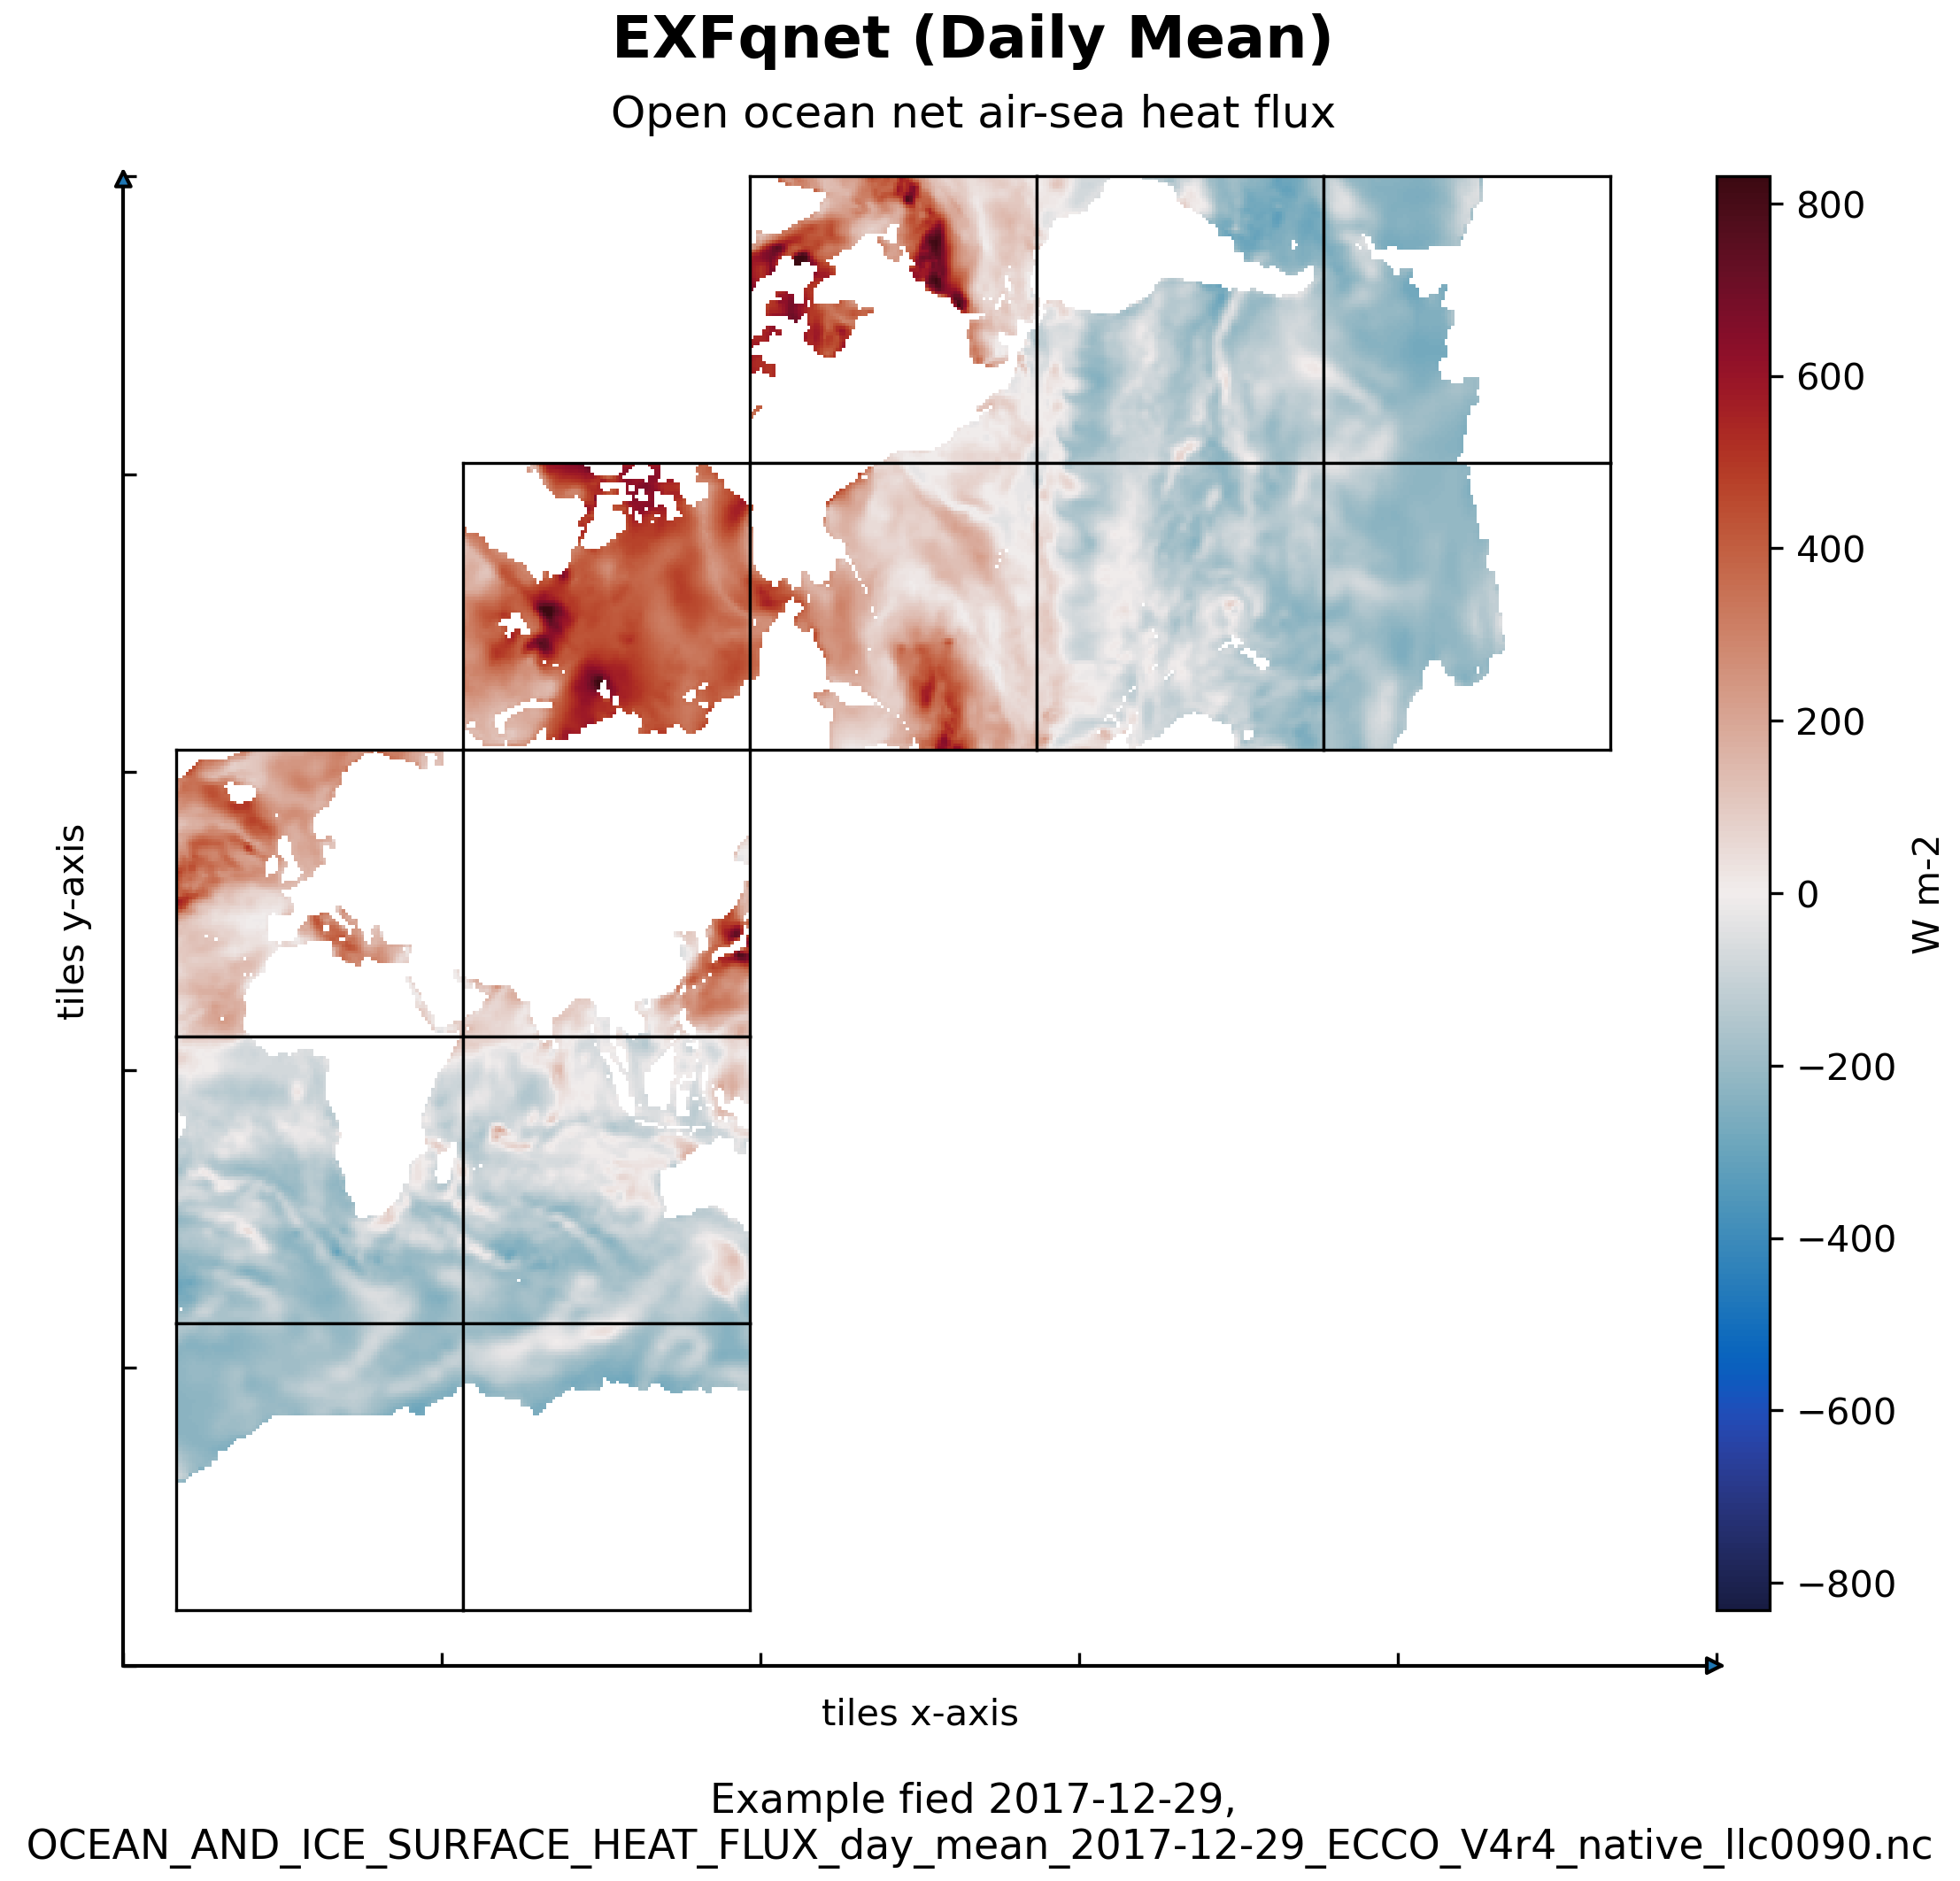
\includegraphics[scale=0.5]{../images/plots/native_plots/Ocean_and_Sea-Ice_Surface_Heat_Fluxes/EXFqnet.png}
\caption{\\Dataset: OCEAN\_AND\_ICE\_SURFACE\_HEAT\_FLUX\\Variable: EXFqnet}
\label{tab:table-OCEAN_AND_ICE_SURFACE_HEAT_FLUX_EXFqnet-Plot}
\end{figure}
\pagebreak
\subsubsection{Native Variable EXFswdn}
\begin{longtable}{|p{0.06\textwidth}|p{0.41\textwidth}|p{0.39\textwidth}|p{0.06\textwidth}|}
\caption{CDL description of OCEAN\_AND\_ICE\_SURFACE\_HEAT\_FLUX's EXFswdn variable}
\label{tab:table-OCEAN_AND_ICE_SURFACE_HEAT_FLUX_EXFswdn} \\ 
\hline \endhead \hline \endfoot
\rowcolor{lightgray} \textbf{Storage Type} & \textbf{Variable Name} & \textbf{Description} & \textbf{Unit} \\ \hline
float32 & EXFswdn & Downwelling shortwave radiative flux & W m-2 \\ \hline
\rowcolor{lightgray}  \multicolumn{4}{|p{1.00\textwidth}|}{\textbf{CDL Description}} \\ \hline
\multicolumn{4}{|p{1.00\textwidth}|}{\makecell{\parbox{1\textwidth}{float32 EXFswdn(time, tile, j, i)\\
\hspace*{0.5cm}EXFswdn: \_FillValue = 9.96921e+36\\
\hspace*{0.5cm}EXFswdn: long\_name = Downwelling shortwave radiative flux\\
\hspace*{0.5cm}EXFswdn: units = W m: 2\\
\hspace*{0.5cm}EXFswdn: coverage\_content\_type = modelResult\\
\hspace*{0.5cm}EXFswdn: direction = >0 increases potential temperature (THETA)\\
\hspace*{0.5cm}EXFswdn: standard\_name = surface\_downwelling\_shortwave\_flux\_in\_air\\
\hspace*{0.5cm}EXFswdn: coordinates = XC time YC\\
\hspace*{0.5cm}EXFswdn: valid\_min = : 224.63368225097656\\
\hspace*{0.5cm}EXFswdn: valid\_max = 707.345947265625}}} \\ \hline
\rowcolor{lightgray} \multicolumn{4}{|p{1.00\textwidth}|}{\textbf{Comments}} \\ \hline
\multicolumn{4}{|p{1\textwidth}|}{Downward shortwave radiative flux. Note: sum of ERA-Interim downward shortwave radiation and the control adjustment from ocean state estimation.} \\ \hline
\end{longtable}

\begin{figure}[H]
\centering
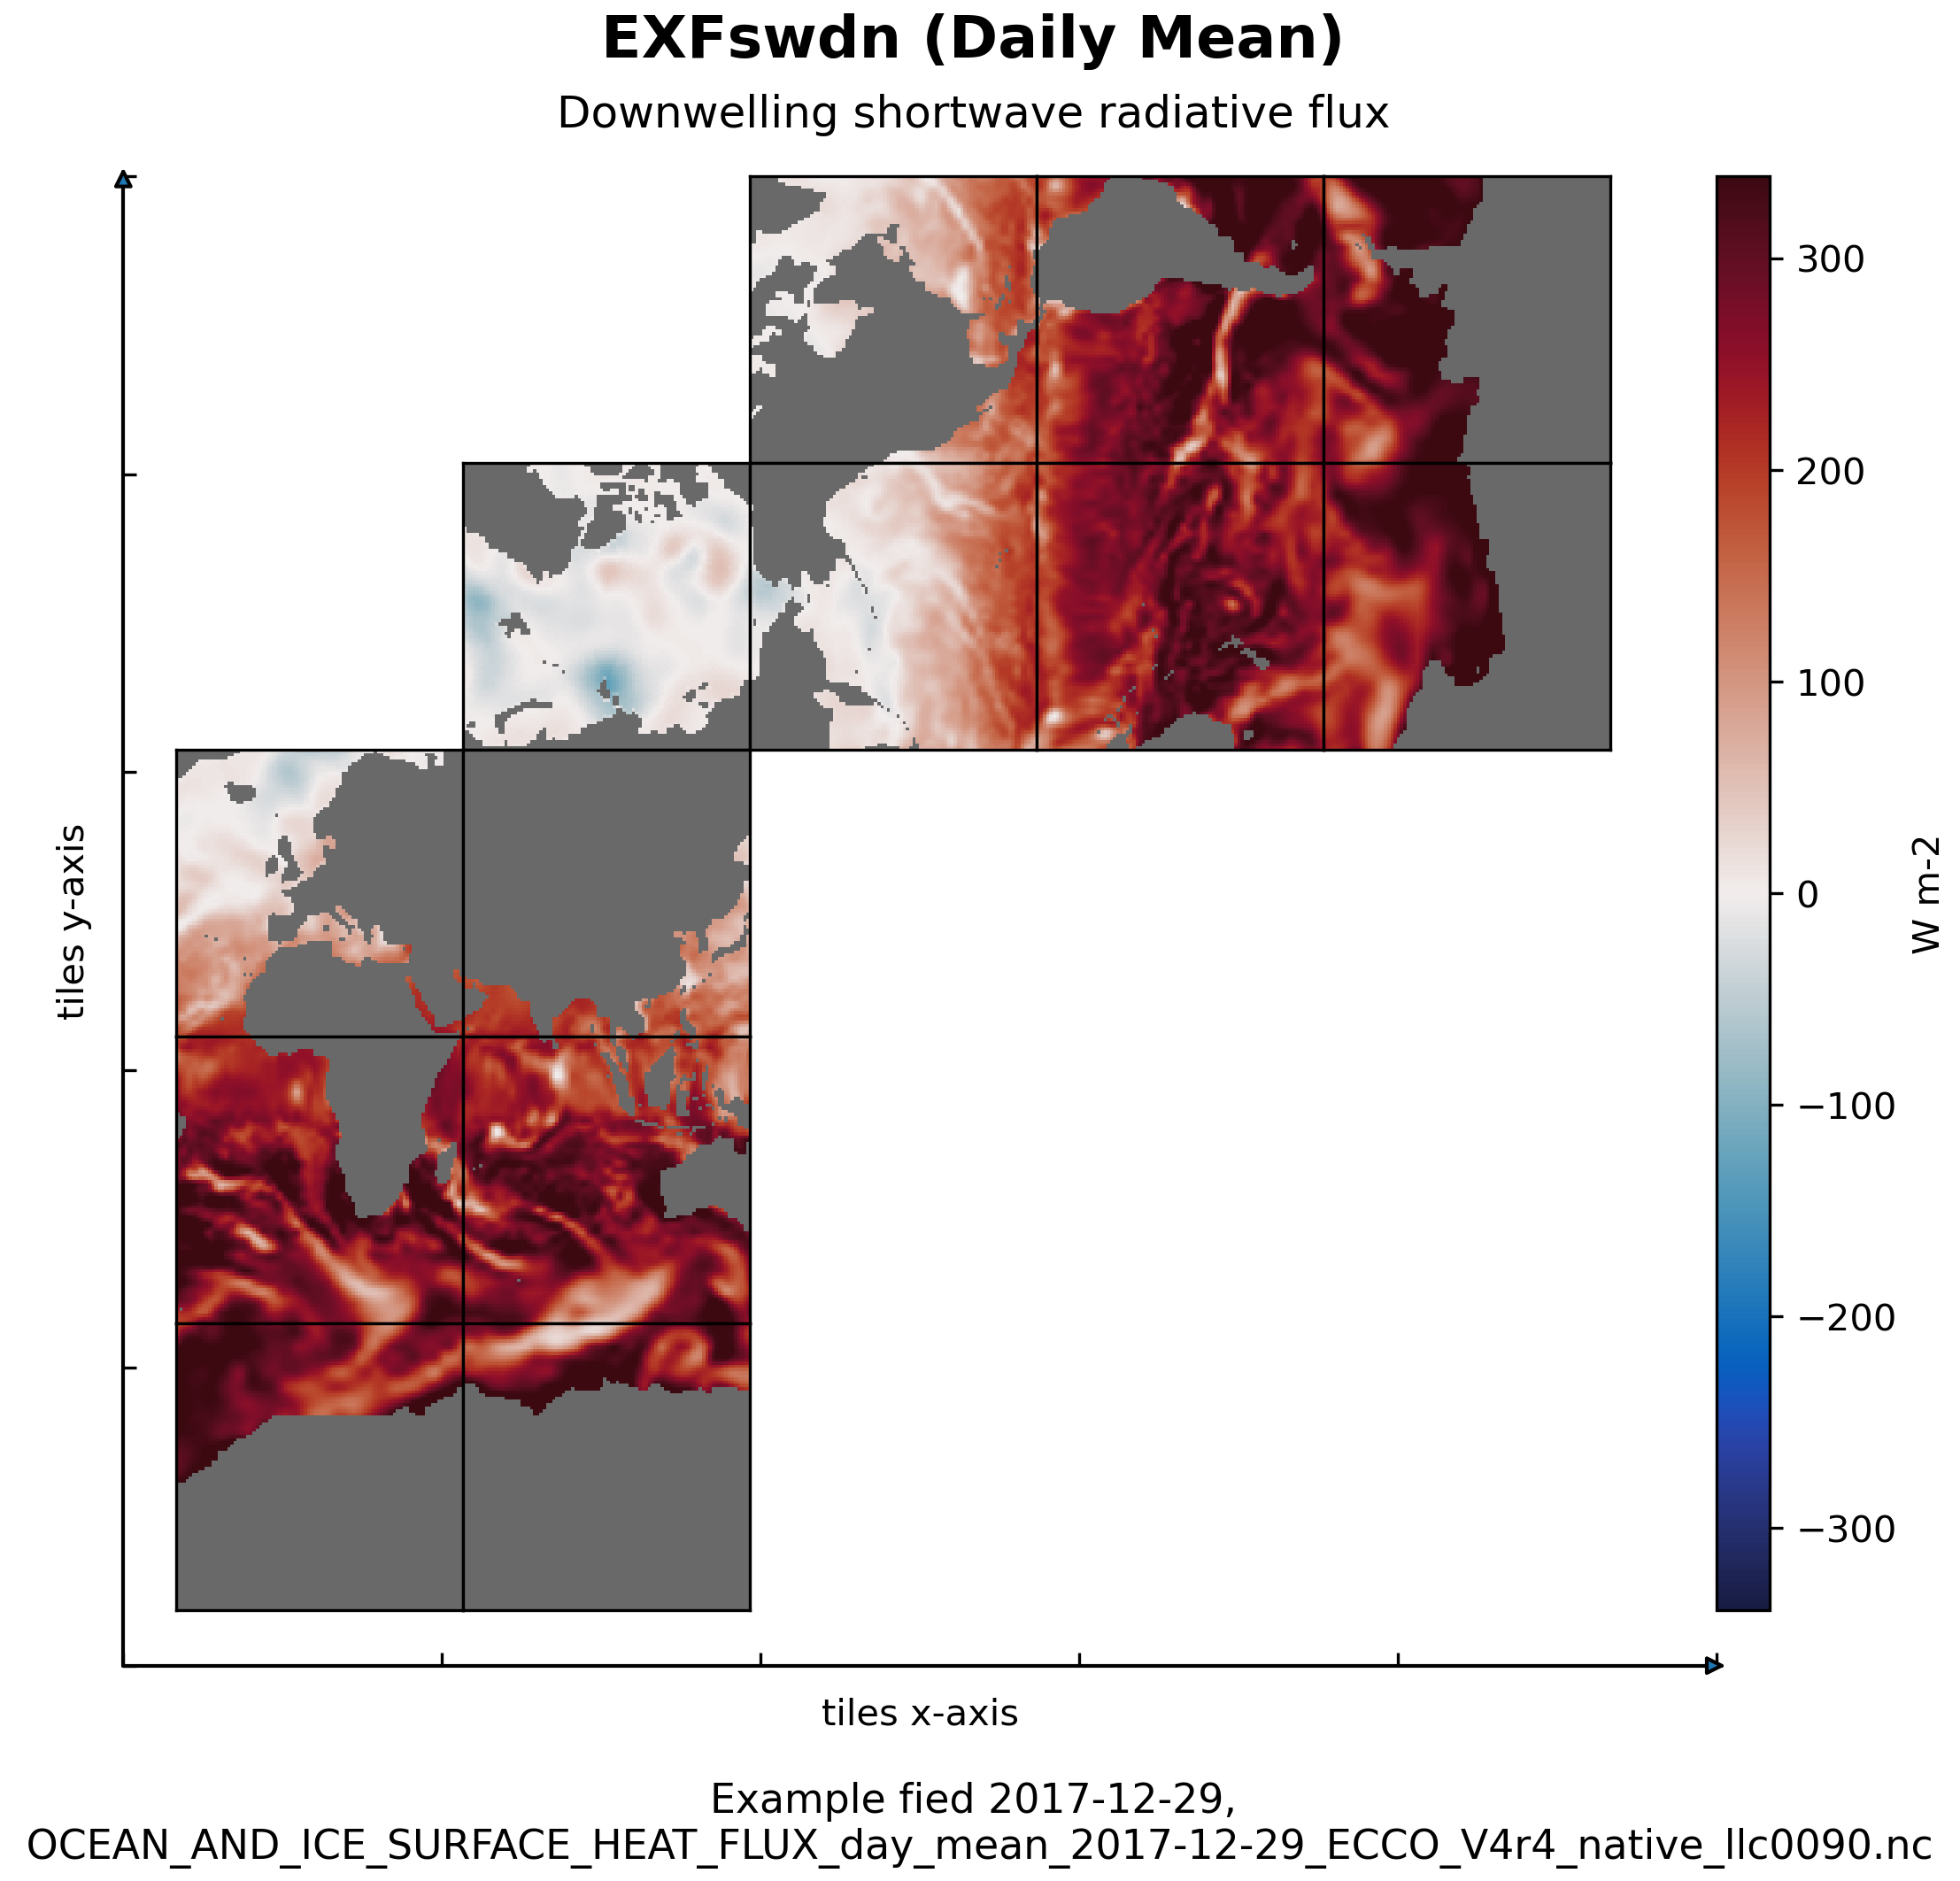
\includegraphics[scale=0.5]{../images/plots/native_plots/Ocean_and_Sea-Ice_Surface_Heat_Fluxes/EXFswdn.png}
\caption{\\Dataset: OCEAN\_AND\_ICE\_SURFACE\_HEAT\_FLUX\\Variable: EXFswdn}
\label{tab:table-OCEAN_AND_ICE_SURFACE_HEAT_FLUX_EXFswdn-Plot}
\end{figure}
\pagebreak
\subsubsection{Native Variable EXFswnet}
\begin{longtable}{|p{0.06\textwidth}|p{0.41\textwidth}|p{0.39\textwidth}|p{0.06\textwidth}|}
\caption{CDL description of OCEAN\_AND\_ICE\_SURFACE\_HEAT\_FLUX's EXFswnet variable}
\label{tab:table-OCEAN_AND_ICE_SURFACE_HEAT_FLUX_EXFswnet} \\ 
\hline \endhead \hline \endfoot
\rowcolor{lightgray} \textbf{Storage Type} & \textbf{Variable Name} & \textbf{Description} & \textbf{Unit} \\ \hline
float32 & EXFswnet & Open ocean net shortwave radiative flux & W m-2 \\ \hline
\rowcolor{lightgray}  \multicolumn{4}{|p{1.00\textwidth}|}{\textbf{CDL Description}} \\ \hline
\multicolumn{4}{|p{1.00\textwidth}|}{\makecell{\parbox{1\textwidth}{float32 EXFswnet(time, tile, j, i)\\
\hspace*{0.5cm}EXFswnet: \_FillValue = 9.96921e+36\\
\hspace*{0.5cm}EXFswnet: long\_name = Open ocean net shortwave radiative flux\\
\hspace*{0.5cm}EXFswnet: units = W m: 2\\
\hspace*{0.5cm}EXFswnet: coverage\_content\_type = modelResult\\
\hspace*{0.5cm}EXFswnet: direction = >0 increases potential temperature (THETA)\\
\hspace*{0.5cm}EXFswnet: standard\_name = surface\_net\_downward\_shortwave\_flux\\
\hspace*{0.5cm}EXFswnet: coordinates = XC time YC\\
\hspace*{0.5cm}EXFswnet: valid\_min = : 655.6171264648438\\
\hspace*{0.5cm}EXFswnet: valid\_max = 194.18458557128906}}} \\ \hline
\rowcolor{lightgray} \multicolumn{4}{|p{1.00\textwidth}|}{\textbf{Comments}} \\ \hline
\multicolumn{4}{|p{1\textwidth}|}{Net shortwave radiative flux per unit area of open water (not covered by sea-ice). Note: net shortwave radiation over open water calculated from downward shortwave flux (EXFswdn) and ocean surface albdeo.} \\ \hline
\end{longtable}

\begin{figure}[H]
\centering
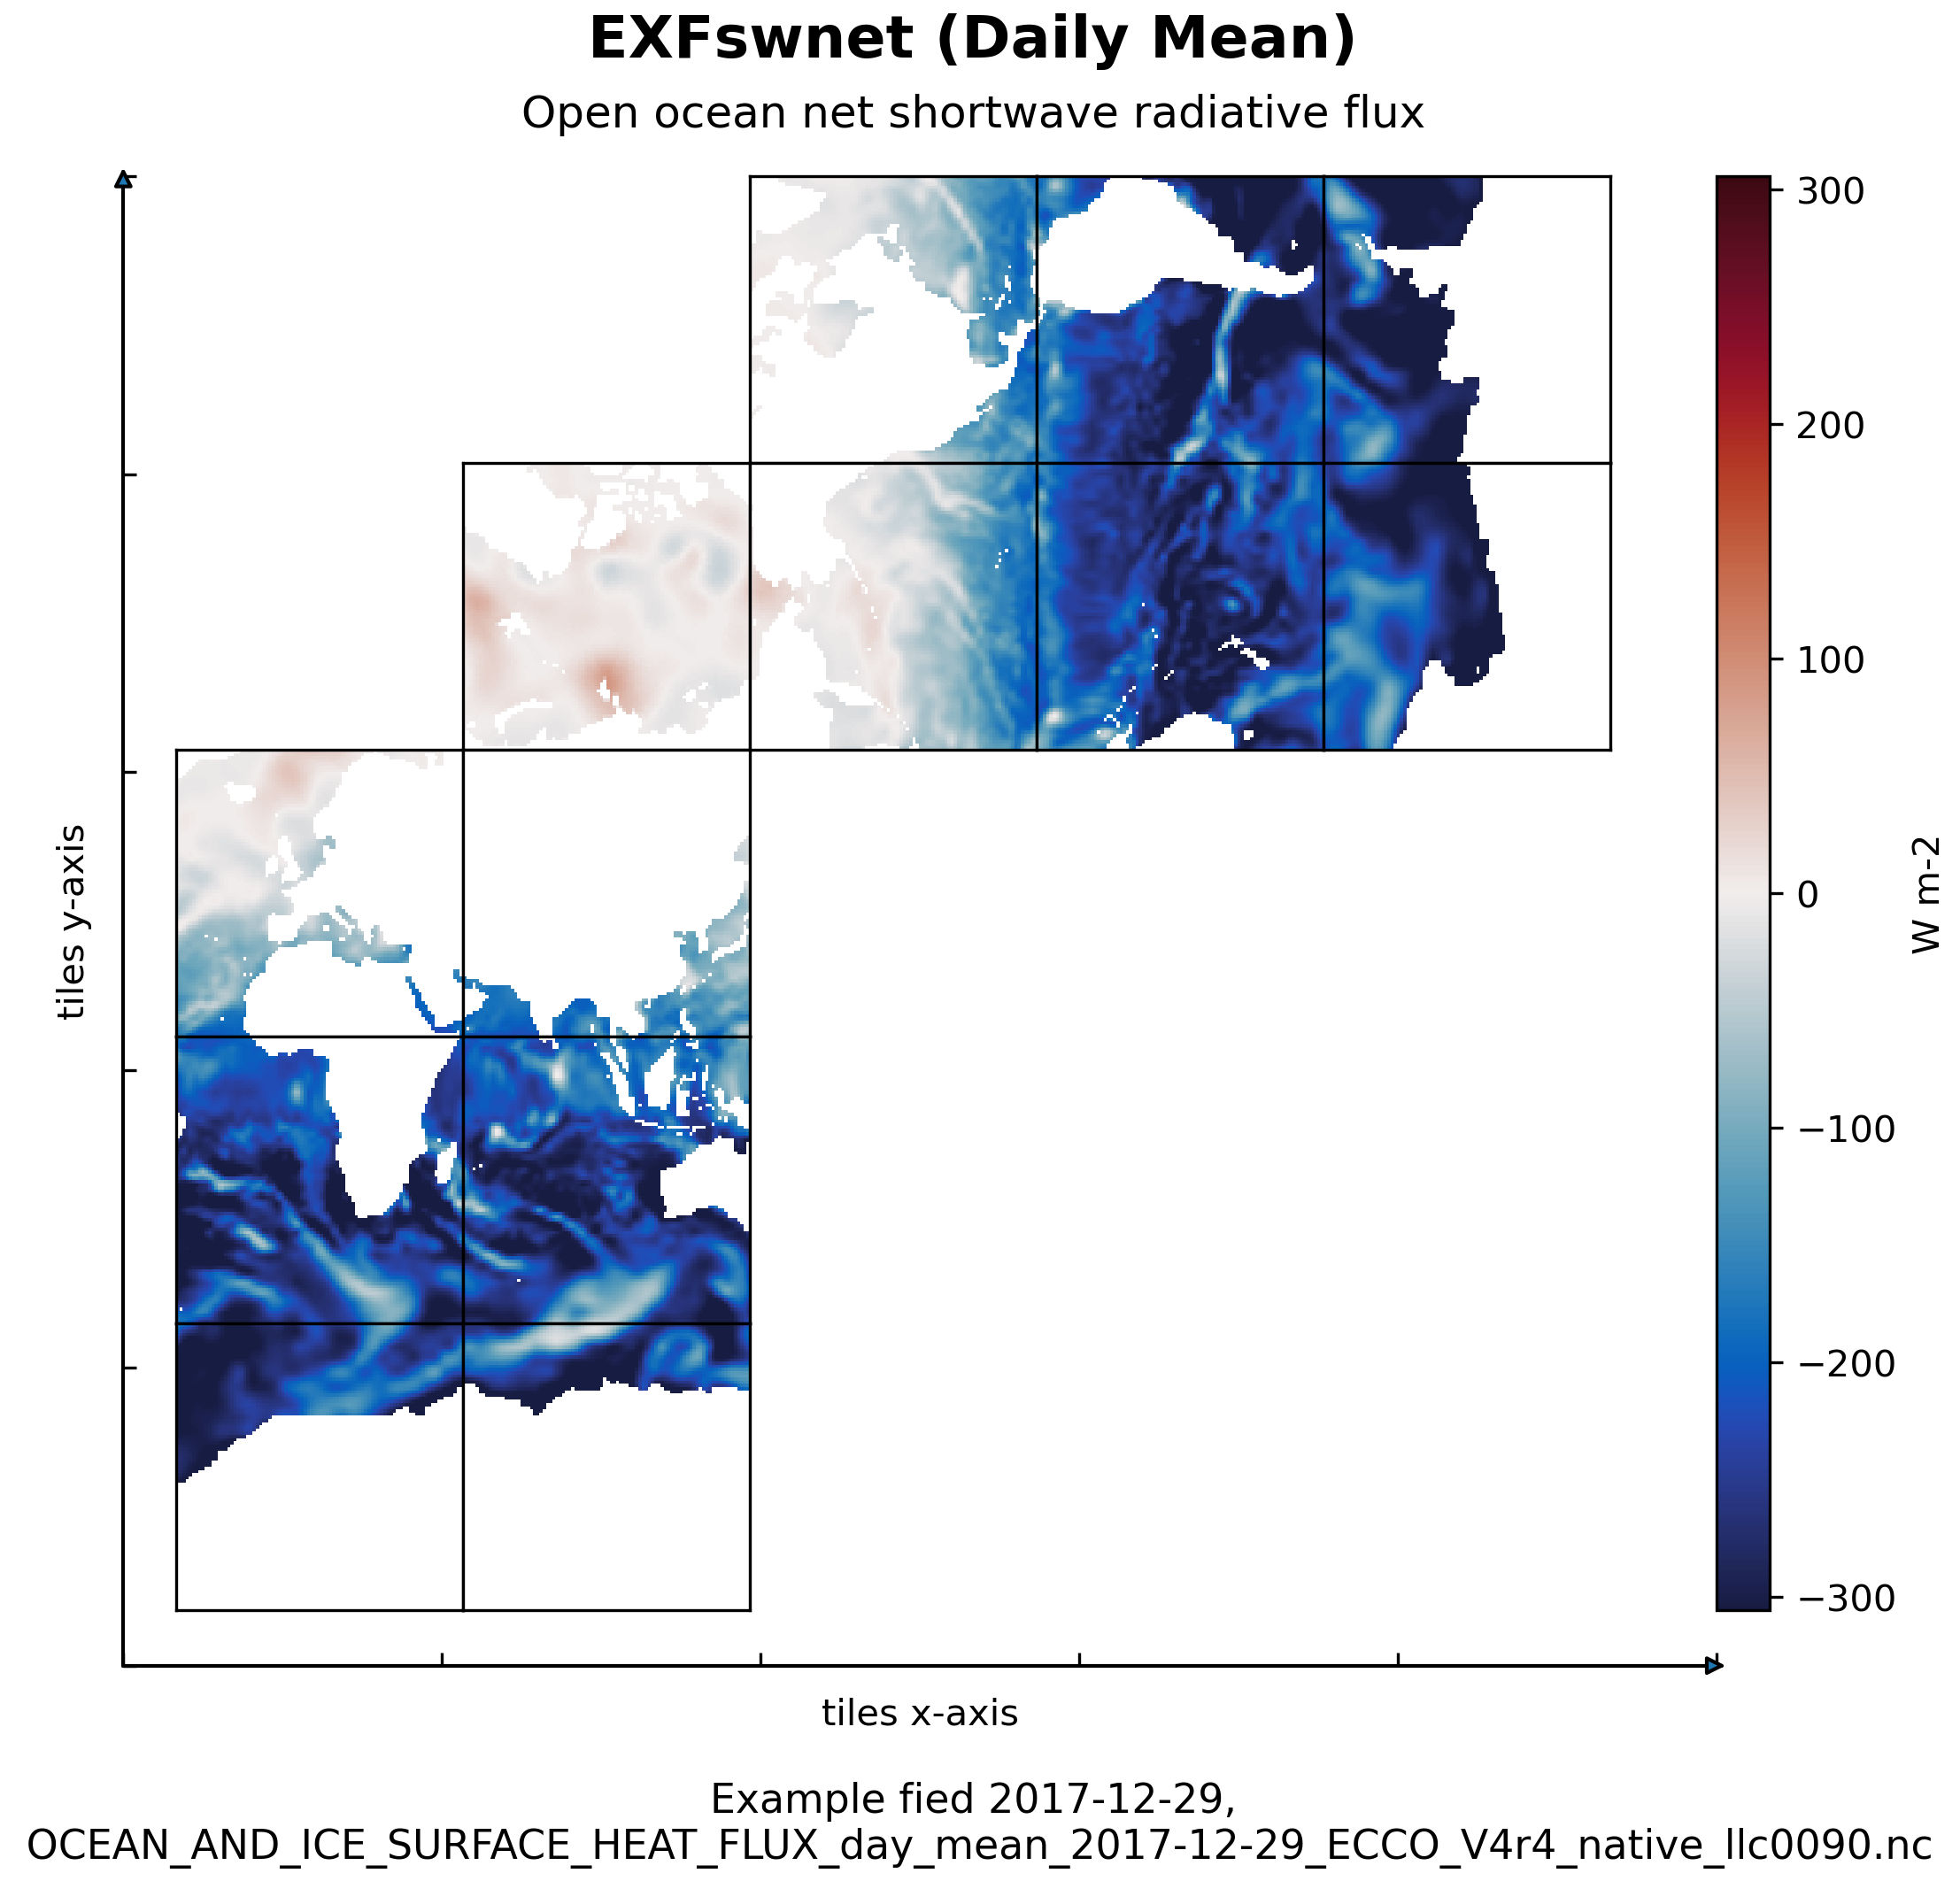
\includegraphics[scale=0.5]{../images/plots/native_plots/Ocean_and_Sea-Ice_Surface_Heat_Fluxes/EXFswnet.png}
\caption{\\Dataset: OCEAN\_AND\_ICE\_SURFACE\_HEAT\_FLUX\\Variable: EXFswnet}
\label{tab:table-OCEAN_AND_ICE_SURFACE_HEAT_FLUX_EXFswnet-Plot}
\end{figure}
\pagebreak
\subsubsection{Native Variable SIaaflux}
\begin{longtable}{|p{0.06\textwidth}|p{0.41\textwidth}|p{0.39\textwidth}|p{0.06\textwidth}|}
\caption{CDL description of OCEAN\_AND\_ICE\_SURFACE\_HEAT\_FLUX's SIaaflux variable}
\label{tab:table-OCEAN_AND_ICE_SURFACE_HEAT_FLUX_SIaaflux} \\ 
\hline \endhead \hline \endfoot
\rowcolor{lightgray} \textbf{Storage Type} & \textbf{Variable Name} & \textbf{Description} & \textbf{Unit} \\ \hline
float32 & SIaaflux & Conservative ocean and sea-ice advective heat flux adjustment & W m-2 \\ \hline
\rowcolor{lightgray}  \multicolumn{4}{|p{1.00\textwidth}|}{\textbf{CDL Description}} \\ \hline
\multicolumn{4}{|p{1.00\textwidth}|}{\makecell{\parbox{1\textwidth}{float32 SIaaflux(time, tile, j, i)\\
\hspace*{0.5cm}SIaaflux: \_FillValue = 9.96921e+36\\
\hspace*{0.5cm}SIaaflux: long\_name = Conservative ocean and sea: ice advective heat flux adjustment\\
\hspace*{0.5cm}SIaaflux: units = W m: 2\\
\hspace*{0.5cm}SIaaflux: coverage\_content\_type = modelResult\\
\hspace*{0.5cm}SIaaflux: direction = >0 decrease potential temperature (THETA)\\
\hspace*{0.5cm}SIaaflux: coordinates = XC time YC\\
\hspace*{0.5cm}SIaaflux: valid\_min = : 16.214622497558594\\
\hspace*{0.5cm}SIaaflux: valid\_max = 50.35451889038086}}} \\ \hline
\rowcolor{lightgray} \multicolumn{4}{|p{1.00\textwidth}|}{\textbf{Comments}} \\ \hline
\multicolumn{4}{|p{1\textwidth}|}{Heat flux associated with the temperature difference between sea surface temperature and sea-ice (assume 0 degree C in the model). Note: heat flux needed to melt/freeze sea-ice at 0 degC to sea water at the ocean surface (at sea surface temperature), excluding the latent heat of fusion.} \\ \hline
\end{longtable}

\begin{figure}[H]
\centering
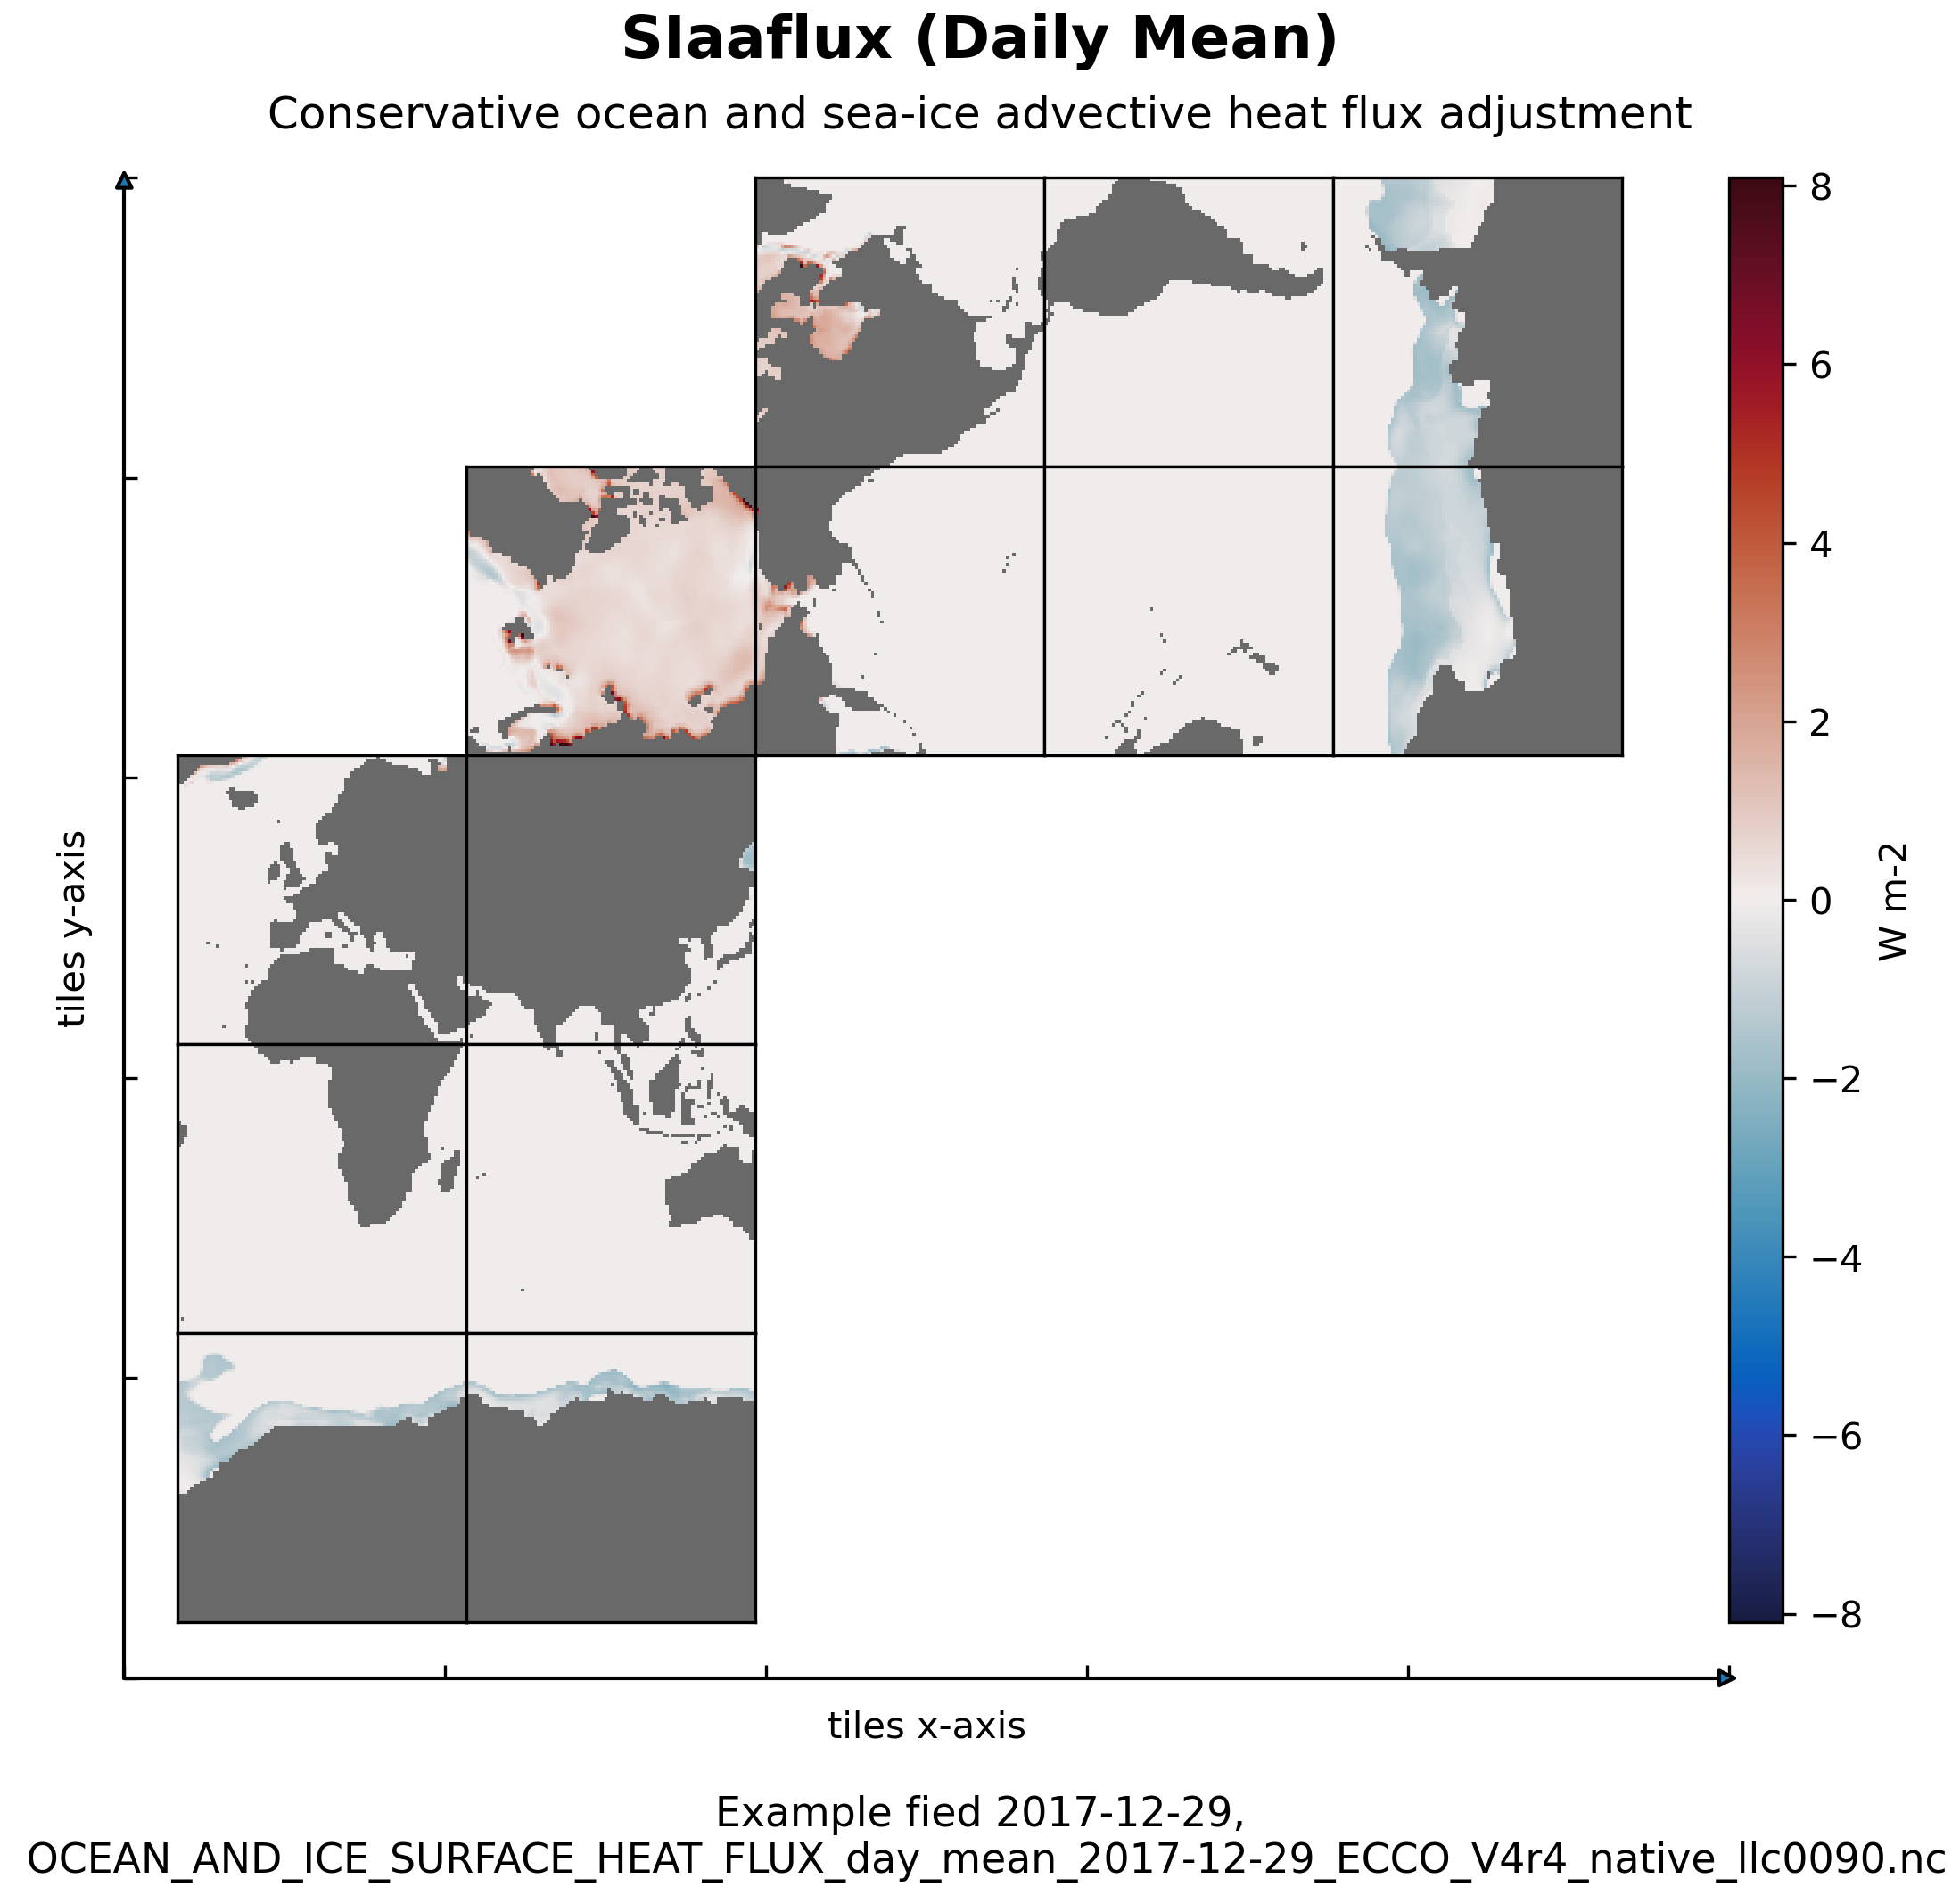
\includegraphics[scale=0.5]{../images/plots/native_plots/Ocean_and_Sea-Ice_Surface_Heat_Fluxes/SIaaflux.png}
\caption{\\Dataset: OCEAN\_AND\_ICE\_SURFACE\_HEAT\_FLUX\\Variable: SIaaflux}
\label{tab:table-OCEAN_AND_ICE_SURFACE_HEAT_FLUX_SIaaflux-Plot}
\end{figure}
\pagebreak
\subsubsection{Native Variable SIatmQnt}
\begin{longtable}{|p{0.06\textwidth}|p{0.41\textwidth}|p{0.39\textwidth}|p{0.06\textwidth}|}
\caption{CDL description of OCEAN\_AND\_ICE\_SURFACE\_HEAT\_FLUX's SIatmQnt variable}
\label{tab:table-OCEAN_AND_ICE_SURFACE_HEAT_FLUX_SIatmQnt} \\ 
\hline \endhead \hline \endfoot
\rowcolor{lightgray} \textbf{Storage Type} & \textbf{Variable Name} & \textbf{Description} & \textbf{Unit} \\ \hline
float32 & SIatmQnt & Net upward heat flux to the atmosphere & W m-2 \\ \hline
\rowcolor{lightgray}  \multicolumn{4}{|p{1.00\textwidth}|}{\textbf{CDL Description}} \\ \hline
\multicolumn{4}{|p{1.00\textwidth}|}{\makecell{\parbox{1\textwidth}{float32 SIatmQnt(time, tile, j, i)\\
\hspace*{0.5cm}SIatmQnt: \_FillValue = 9.96921e+36\\
\hspace*{0.5cm}SIatmQnt: long\_name = Net upward heat flux to the atmosphere\\
\hspace*{0.5cm}SIatmQnt: units = W m: 2\\
\hspace*{0.5cm}SIatmQnt: coverage\_content\_type = modelResult\\
\hspace*{0.5cm}SIatmQnt: direction = >0 upward\\
decreases ocean temperature\\
\hspace*{0.5cm}SIatmQnt: standard\_name = surface\_upward\_heat\_flux\_in\_air\\
\hspace*{0.5cm}SIatmQnt: coordinates = XC time YC\\
\hspace*{0.5cm}SIatmQnt: valid\_min = : 756.0607299804688\\
\hspace*{0.5cm}SIatmQnt: valid\_max = 1704.7703857421875}}} \\ \hline
\rowcolor{lightgray} \multicolumn{4}{|p{1.00\textwidth}|}{\textbf{Comments}} \\ \hline
\multicolumn{4}{|p{1\textwidth}|}{Net upward heat flux to the atmosphere across open water and sea-ice or snow surfaces. Note: nonzero SIatmQnt may not be associated with a change in ocean potential temperature due to sea-ice growth or melting. To calculate total ocean heat content changes use the variable TFLUX which also accounts for changing ocean mass (e.g. oceFWflx).} \\ \hline
\end{longtable}

\begin{figure}[H]
\centering
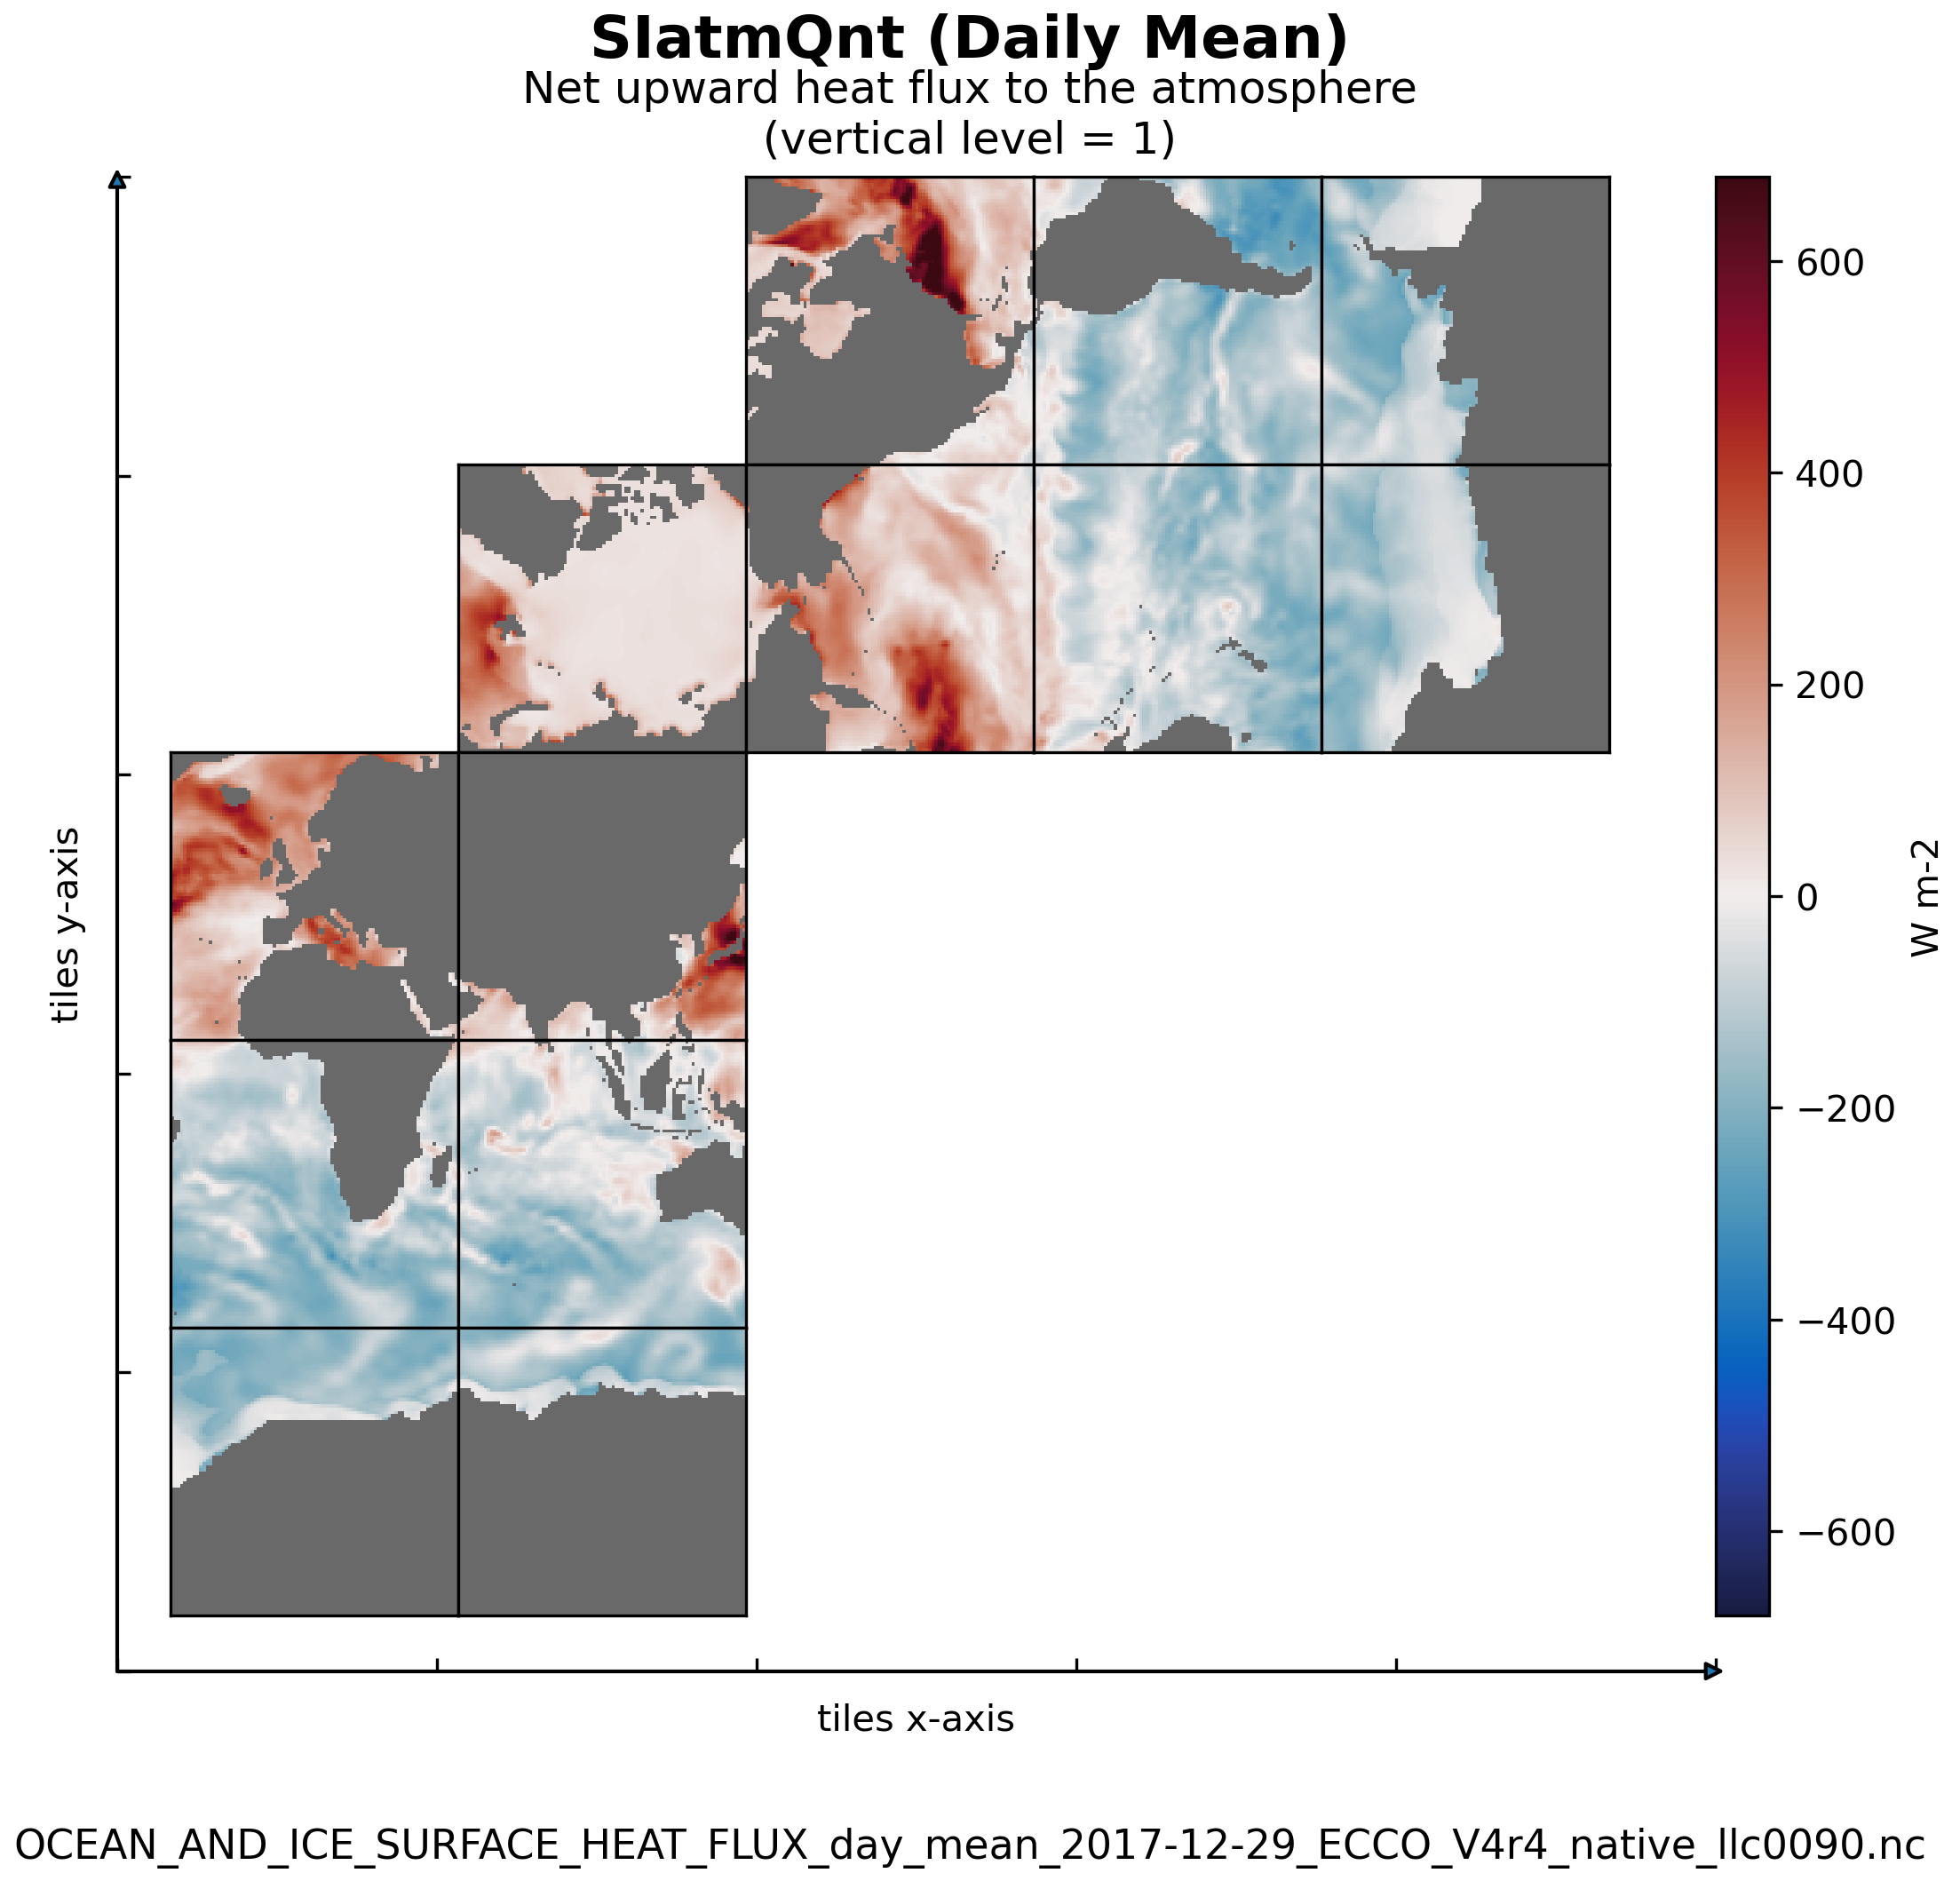
\includegraphics[scale=0.5]{../images/plots/native_plots/Ocean_and_Sea-Ice_Surface_Heat_Fluxes/SIatmQnt.png}
\caption{\\Dataset: OCEAN\_AND\_ICE\_SURFACE\_HEAT\_FLUX\\Variable: SIatmQnt}
\label{tab:table-OCEAN_AND_ICE_SURFACE_HEAT_FLUX_SIatmQnt-Plot}
\end{figure}
\pagebreak
\subsubsection{Native Variable TFLUX}
\begin{longtable}{|p{0.06\textwidth}|p{0.41\textwidth}|p{0.39\textwidth}|p{0.06\textwidth}|}
\caption{CDL description of OCEAN\_AND\_ICE\_SURFACE\_HEAT\_FLUX's TFLUX variable}
\label{tab:table-OCEAN_AND_ICE_SURFACE_HEAT_FLUX_TFLUX} \\ 
\hline \endhead \hline \endfoot
\rowcolor{lightgray} \textbf{Storage Type} & \textbf{Variable Name} & \textbf{Description} & \textbf{Unit} \\ \hline
float32 & TFLUX & Rate of change of ocean heat content per m2 accounting for mass fluxes. & W m-2 \\ \hline
\rowcolor{lightgray}  \multicolumn{4}{|p{1.00\textwidth}|}{\textbf{CDL Description}} \\ \hline
\multicolumn{4}{|p{1.00\textwidth}|}{\makecell{\parbox{1\textwidth}{float32 TFLUX(time, tile, j, i)\\
\hspace*{0.5cm}TFLUX: \_FillValue = 9.96921e+36\\
\hspace*{0.5cm}TFLUX: long\_name = Rate of change of ocean heat content per m2 accounting for mass fluxes.\\
\hspace*{0.5cm}TFLUX: units = W m: 2\\
\hspace*{0.5cm}TFLUX: coverage\_content\_type = modelResult\\
\hspace*{0.5cm}TFLUX: direction = >0 increases potential temperature (THETA)\\
\hspace*{0.5cm}TFLUX: coordinates = XC time YC\\
\hspace*{0.5cm}TFLUX: valid\_min = : 1713.51220703125\\
\hspace*{0.5cm}TFLUX: valid\_max = 870.3130493164062}}} \\ \hline
\rowcolor{lightgray} \multicolumn{4}{|p{1.00\textwidth}|}{\textbf{Comments}} \\ \hline
\multicolumn{4}{|p{1\textwidth}|}{The rate of change of ocean heat content due to heat fluxes across the liquid surface and the addition or removal of mass. . Note: the global area integral of TFLUX and geothermal flux (geothermalFlux.bin) matches the time-derivative of ocean heat content (J/s). Unlike oceQnet, TFLUX includes the contribution to the ocean heat content from changing ocean mass (e.g. from oceFWflx).} \\ \hline
\end{longtable}

\begin{figure}[H]
\centering
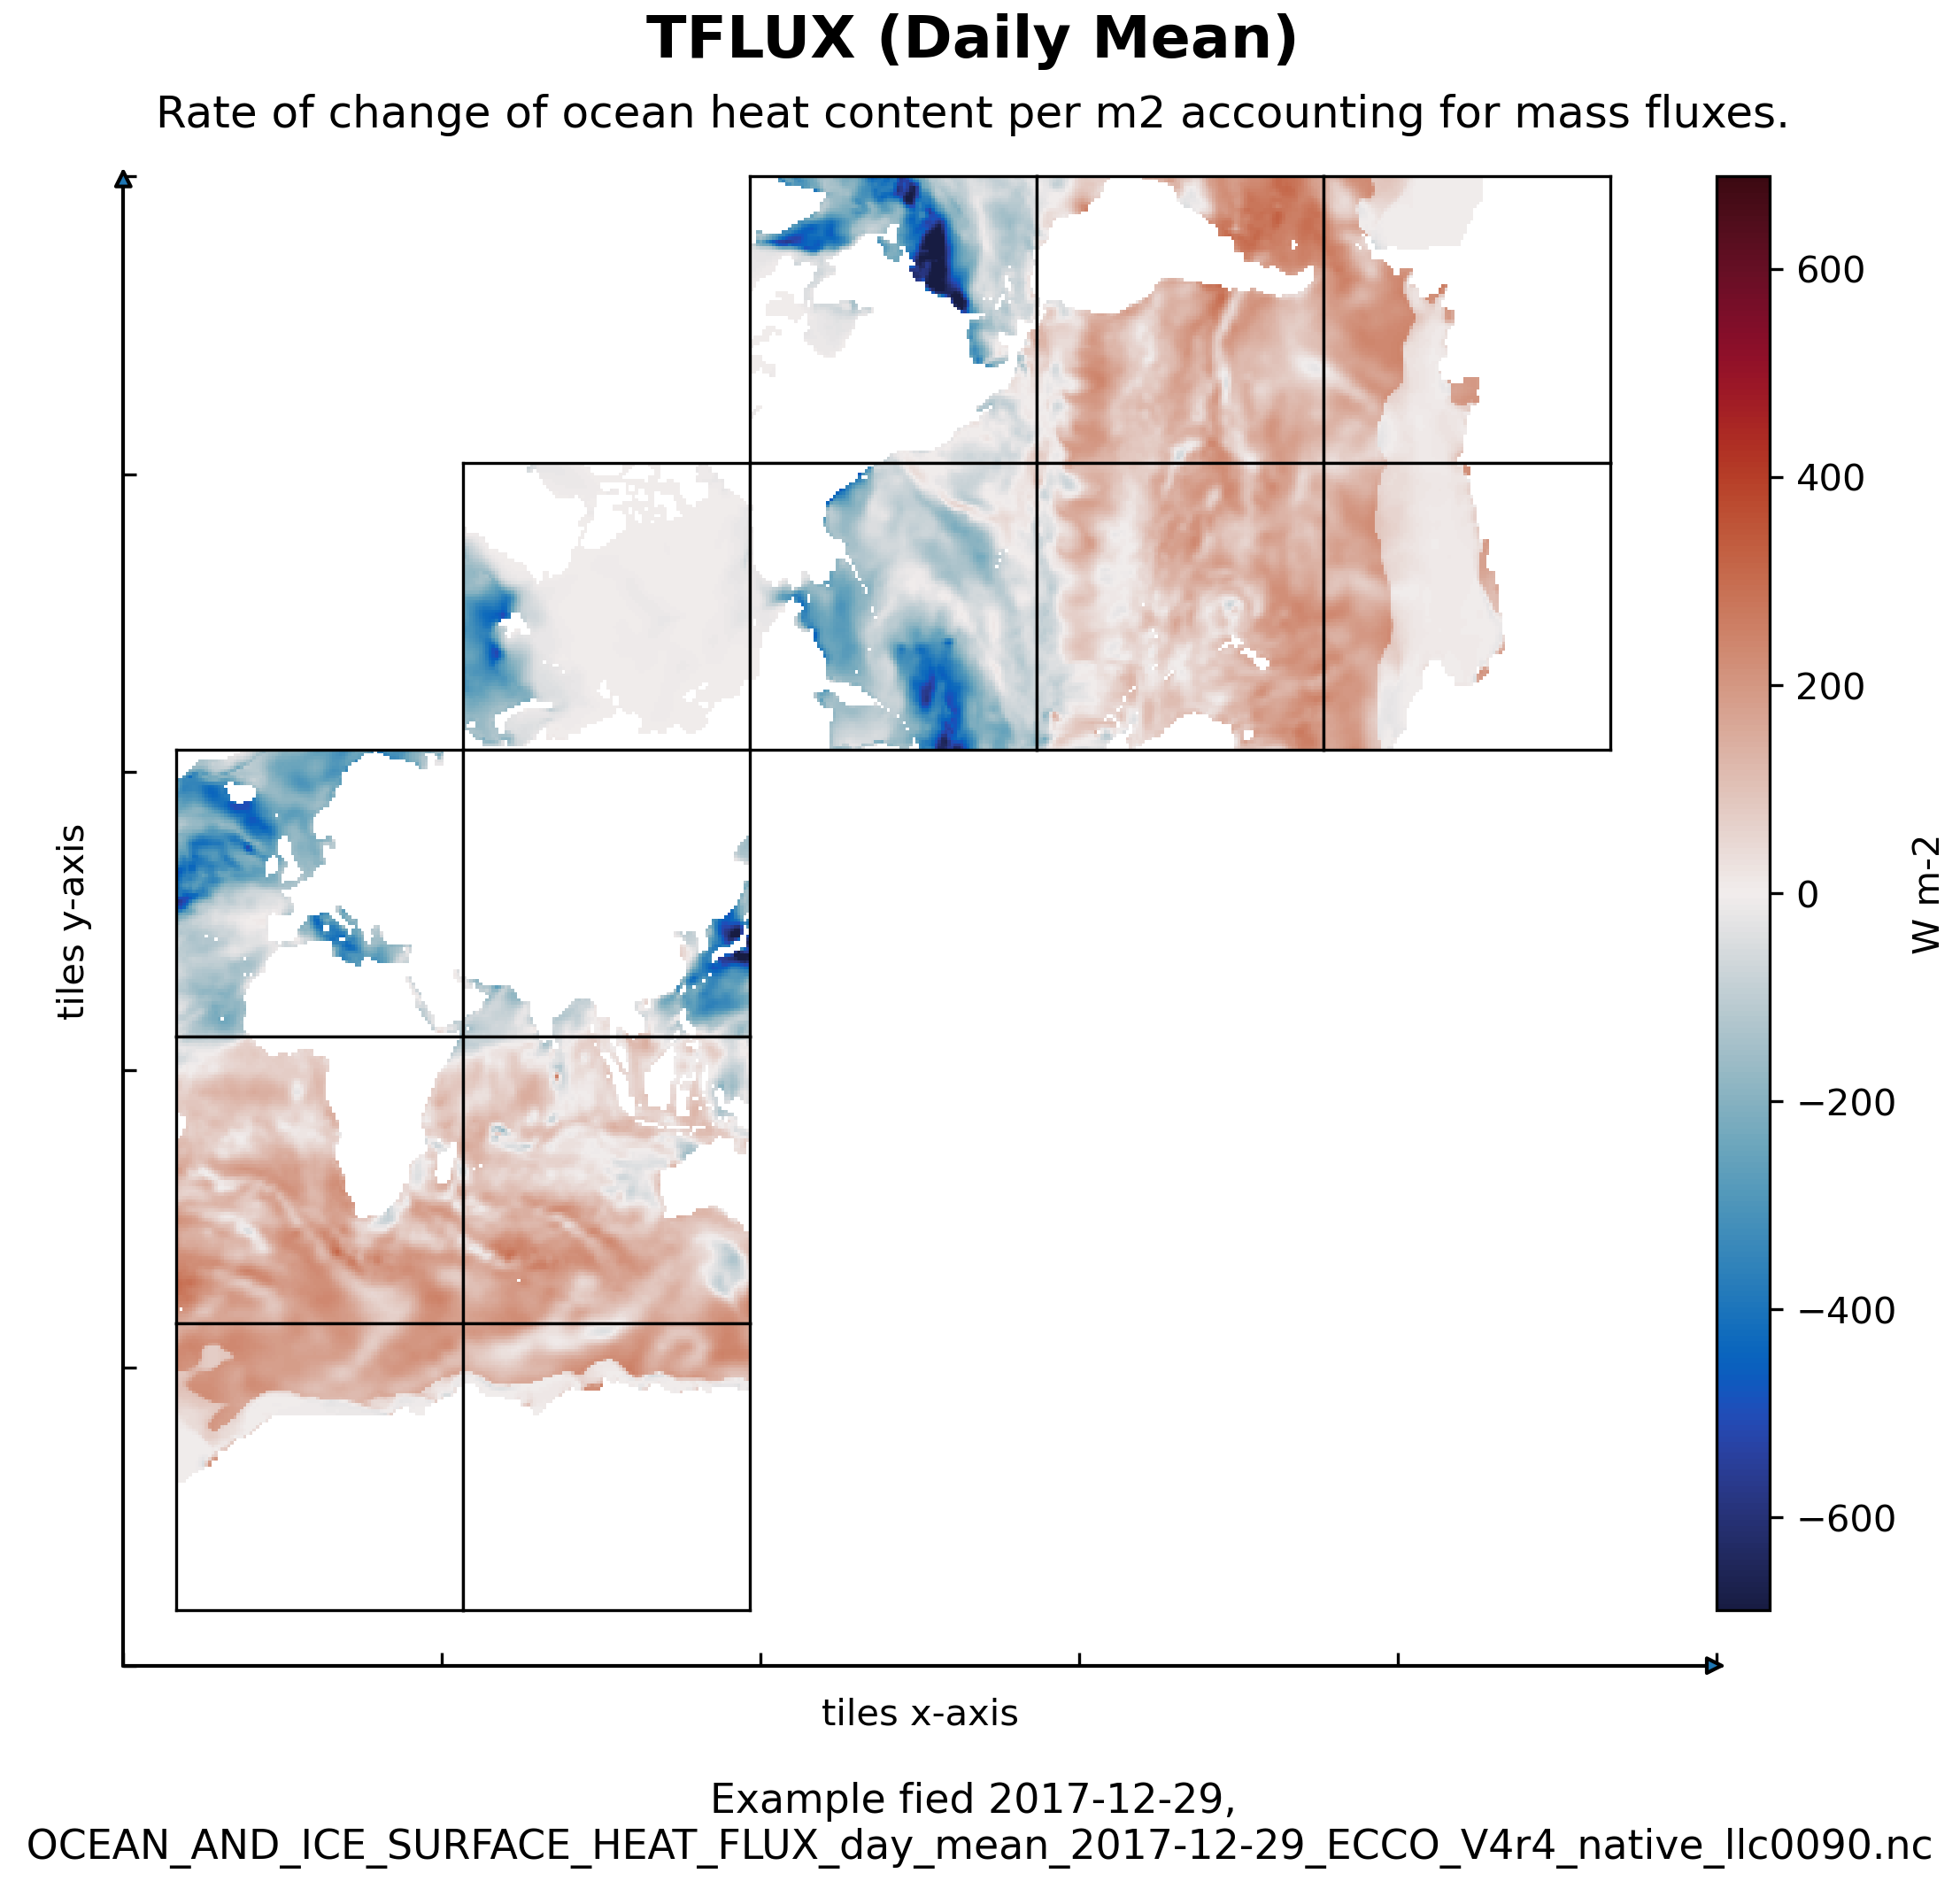
\includegraphics[scale=0.5]{../images/plots/native_plots/Ocean_and_Sea-Ice_Surface_Heat_Fluxes/TFLUX.png}
\caption{\\Dataset: OCEAN\_AND\_ICE\_SURFACE\_HEAT\_FLUX\\Variable: TFLUX}
\label{tab:table-OCEAN_AND_ICE_SURFACE_HEAT_FLUX_TFLUX-Plot}
\end{figure}
\pagebreak
\subsubsection{Native Variable oceQnet}
\begin{longtable}{|p{0.06\textwidth}|p{0.41\textwidth}|p{0.39\textwidth}|p{0.06\textwidth}|}
\caption{CDL description of OCEAN\_AND\_ICE\_SURFACE\_HEAT\_FLUX's oceQnet variable}
\label{tab:table-OCEAN_AND_ICE_SURFACE_HEAT_FLUX_oceQnet} \\ 
\hline \endhead \hline \endfoot
\rowcolor{lightgray} \textbf{Storage Type} & \textbf{Variable Name} & \textbf{Description} & \textbf{Unit} \\ \hline
float32 & oceQnet & Net heat flux into the ocean surface & W m-2 \\ \hline
\rowcolor{lightgray}  \multicolumn{4}{|p{1.00\textwidth}|}{\textbf{CDL Description}} \\ \hline
\multicolumn{4}{|p{1.00\textwidth}|}{\makecell{\parbox{1\textwidth}{float32 oceQnet(time, tile, j, i)\\
\hspace*{0.5cm}oceQnet: \_FillValue = 9.96921e+36\\
\hspace*{0.5cm}oceQnet: long\_name = Net heat flux into the ocean surface\\
\hspace*{0.5cm}oceQnet: units = W m: 2\\
\hspace*{0.5cm}oceQnet: coverage\_content\_type = modelResult\\
\hspace*{0.5cm}oceQnet: direction = >0 increases potential temperature (THETA)\\
\hspace*{0.5cm}oceQnet: standard\_name = surface\_downward\_heat\_flux\_in\_sea\_water\\
\hspace*{0.5cm}oceQnet: coordinates = XC time YC\\
\hspace*{0.5cm}oceQnet: valid\_min = : 1708.8460693359375\\
\hspace*{0.5cm}oceQnet: valid\_max = 675.3716430664062}}} \\ \hline
\rowcolor{lightgray} \multicolumn{4}{|p{1.00\textwidth}|}{\textbf{Comments}} \\ \hline
\multicolumn{4}{|p{1\textwidth}|}{Net heat flux into the ocean surface from all processes: air-sea turbulent and radiative fluxes and turbulent and conductive fluxes between the ocean and sea-ice and snow. Note: oceQnet does not include the change in ocean heat content due to changing ocean ocean mass (oceFWflx). Mass fluxes from evaporation, precipitation, and runoff (EXFempmr) happen at the same temperature as the ocean surface temperature. Consequently, EmPmR does not change ocean surface temperature. Conversely, mass fluxes due to sea-ice thickening/thinning and snow melt in the model are assumed to happen at a fixed 0C. Consequently, mass fluxes due to phase changes between seawater and sea-ice and snow induce a heat flux when the ocean surface temperaure is not 0C. The variable TFLUX does include the change in ocean heat content due to changing ocean mass.} \\ \hline
\end{longtable}

\begin{figure}[H]
\centering
\includegraphics[scale=0.5]{../images/plots/native_plots/Ocean_and_Sea-Ice_Surface_Heat_Fluxes/oceQnet.png}
\caption{\\Dataset: OCEAN\_AND\_ICE\_SURFACE\_HEAT\_FLUX\\Variable: oceQnet}
\label{tab:table-OCEAN_AND_ICE_SURFACE_HEAT_FLUX_oceQnet-Plot}
\end{figure}
\pagebreak
\subsubsection{Native Variable oceQsw}
\begin{longtable}{|p{0.06\textwidth}|p{0.41\textwidth}|p{0.39\textwidth}|p{0.06\textwidth}|}
\caption{CDL description of OCEAN\_AND\_ICE\_SURFACE\_HEAT\_FLUX's oceQsw variable}
\label{tab:table-OCEAN_AND_ICE_SURFACE_HEAT_FLUX_oceQsw} \\ 
\hline \endhead \hline \endfoot
\rowcolor{lightgray} \textbf{Storage Type} & \textbf{Variable Name} & \textbf{Description} & \textbf{Unit} \\ \hline
float32 & oceQsw & Net shortwave radiative flux across the ocean surface & W m-2 \\ \hline
\rowcolor{lightgray}  \multicolumn{4}{|p{1.00\textwidth}|}{\textbf{CDL Description}} \\ \hline
\multicolumn{4}{|p{1.00\textwidth}|}{\makecell{\parbox{1\textwidth}{float32 oceQsw(time, tile, j, i)\\
\hspace*{0.5cm}oceQsw: \_FillValue = 9.96921e+36\\
\hspace*{0.5cm}oceQsw: long\_name = Net shortwave radiative flux across the ocean surface\\
\hspace*{0.5cm}oceQsw: units = W m: 2\\
\hspace*{0.5cm}oceQsw: coverage\_content\_type = modelResult\\
\hspace*{0.5cm}oceQsw: direction = >0 increases potential temperature (THETA)\\
\hspace*{0.5cm}oceQsw: coordinates = XC time YC\\
\hspace*{0.5cm}oceQsw: valid\_min = : 134.39808654785156\\
\hspace*{0.5cm}oceQsw: valid\_max = 655.6171264648438}}} \\ \hline
\rowcolor{lightgray} \multicolumn{4}{|p{1.00\textwidth}|}{\textbf{Comments}} \\ \hline
\multicolumn{4}{|p{1\textwidth}|}{Net shortwave radiative flux across the ocean surface. Note: Shortwave radiation penetrates below the surface grid cell.} \\ \hline
\end{longtable}

\begin{figure}[H]
\centering
\includegraphics[scale=0.5]{../images/plots/native_plots/Ocean_and_Sea-Ice_Surface_Heat_Fluxes/oceQsw.png}
\caption{\\Dataset: OCEAN\_AND\_ICE\_SURFACE\_HEAT\_FLUX\\Variable: oceQsw}
\label{tab:table-OCEAN_AND_ICE_SURFACE_HEAT_FLUX_oceQsw-Plot}
\end{figure}
\pagebreak
\subsection{Native NetCDF OCEAN\_AND\_ICE\_SURFACE\_STRESS}
\newp
\begin{longtable}{|p{0.1\textwidth}|p{0.5\textwidth}|}
\caption{Variables in the dataset OCEAN\_AND\_ICE\_SURFACE\_STRESS}
\label{tab:table-OCEAN_AND_ICE_SURFACE_STRESS-fields} \\ 
\hline \endhead \hline \endfoot
\rowcolor{lightgray} \textbf{Dataset:} & \textbf{OCEAN\_AND\_ICE\_SURFACE\_STRESS} \\ \hline
Field: &EXFtaux \\ \hline
Field: &EXFtauy \\ \hline
Field: &oceTAUX \\ \hline
Field: &oceTAUY \\ \hline
\end{longtable}

\pagebreak
\subsubsection{Native Variable EXFtaux}
\begin{longtable}{|p{0.06\textwidth}|p{0.41\textwidth}|p{0.39\textwidth}|p{0.06\textwidth}|}
\caption{CDL description of OCEAN\_AND\_ICE\_SURFACE\_STRESS's EXFtaux variable}
\label{tab:table-OCEAN_AND_ICE_SURFACE_STRESS_EXFtaux} \\ 
\hline \endhead \hline \endfoot
\rowcolor{lightgray} \textbf{Storage Type} & \textbf{Variable Name} & \textbf{Description} & \textbf{Unit} \\ \hline
float32 & EXFtaux & Wind stress in the model +x direction & N m-2 \\ \hline
\rowcolor{lightgray}  \multicolumn{4}{|p{1.00\textwidth}|}{\textbf{CDL Description}} \\ \hline
\multicolumn{4}{|p{1.00\textwidth}|}{\makecell{\parbox{1\textwidth}{float32 EXFtaux(time, tile, j, i)\\
\hspace*{0.5cm}EXFtaux: \_FillValue = 9.96921e+36\\
\hspace*{0.5cm}EXFtaux: long\_name = Wind stress in the model +x direction\\
\hspace*{0.5cm}EXFtaux: units = N m: 2\\
\hspace*{0.5cm}EXFtaux: coverage\_content\_type = modelResult\\
\hspace*{0.5cm}EXFtaux: direction =  >0 increases horizontal velocity in the +x direction (UVEL)\\
\hspace*{0.5cm}EXFtaux: standard\_name = surface\_downward\_x\_stress\\
\hspace*{0.5cm}EXFtaux: coordinates = time YC XC\\
\hspace*{0.5cm}EXFtaux: valid\_min = : 7.474303722381592\\
\hspace*{0.5cm}EXFtaux: valid\_max = 3.7184090614318848}}} \\ \hline
\rowcolor{lightgray} \multicolumn{4}{|p{1.00\textwidth}|}{\textbf{Comments}} \\ \hline
\multicolumn{4}{|p{1\textwidth}|}{Wind stress in the +x direction at the tracer cell on the native model grid. Note: EXFtaux is the stress applied to the ice-free ocean surface and sea-ice covered surface. When sea-ice is present, the total stress applied to the ocean surface in the +x direction is NOT EXFtaux, but a combination of EXFtaux wind stress in the open water fraction and a stress from sea-ice in the ice-covered fraction (see oceTAUX). EXFtaux is the sum of ERA-Interim stress and the control adjustment from ocean state estimation.} \\ \hline
\end{longtable}

\begin{figure}[H]
\centering
\includegraphics[scale=0.5]{../images/plots/native_plots/Ocean_and_Sea-Ice_Surface_Stress/EXFtaux.png}
\caption{\\Dataset: OCEAN\_AND\_ICE\_SURFACE\_STRESS\\Variable: EXFtaux}
\label{tab:table-OCEAN_AND_ICE_SURFACE_STRESS_EXFtaux-Plot}
\end{figure}
\pagebreak
\subsubsection{Native Variable EXFtauy}
\begin{longtable}{|p{0.06\textwidth}|p{0.41\textwidth}|p{0.39\textwidth}|p{0.06\textwidth}|}
\caption{CDL description of OCEAN\_AND\_ICE\_SURFACE\_STRESS's EXFtauy variable}
\label{tab:table-OCEAN_AND_ICE_SURFACE_STRESS_EXFtauy} \\ 
\hline \endhead \hline \endfoot
\rowcolor{lightgray} \textbf{Storage Type} & \textbf{Variable Name} & \textbf{Description} & \textbf{Unit} \\ \hline
float32 & EXFtauy & Wind stress in the model +y direction & N m-2 \\ \hline
\rowcolor{lightgray}  \multicolumn{4}{|p{1.00\textwidth}|}{\textbf{CDL Description}} \\ \hline
\multicolumn{4}{|p{1.00\textwidth}|}{\makecell{\parbox{1\textwidth}{float32 EXFtauy(time, tile, j, i)\\
\hspace*{0.5cm}EXFtauy: \_FillValue = 9.96921e+36\\
\hspace*{0.5cm}EXFtauy: long\_name = Wind stress in the model +y direction\\
\hspace*{0.5cm}EXFtauy: units = N m: 2\\
\hspace*{0.5cm}EXFtauy: coverage\_content\_type = modelResult\\
\hspace*{0.5cm}EXFtauy: direction =  >0 increases horizontal velocity in the +y direction (VVEL)\\
\hspace*{0.5cm}EXFtauy: standard\_name = surface\_downward\_y\_stress\\
\hspace*{0.5cm}EXFtauy: coordinates = time YC XC\\
\hspace*{0.5cm}EXFtauy: valid\_min = : 3.71972918510437\\
\hspace*{0.5cm}EXFtauy: valid\_max = 3.7044837474823}}} \\ \hline
\rowcolor{lightgray} \multicolumn{4}{|p{1.00\textwidth}|}{\textbf{Comments}} \\ \hline
\multicolumn{4}{|p{1\textwidth}|}{Wind stress in the +y direction at the tracer cell on the native model grid. Note: EXFtauy is the stress applied to the ice-free ocean surface and sea-ice covered surface. When sea-ice is present, the total stress applied to the ocean surface in the +y direction is NOT EXFtauy, but a combination of EXFtauy wind stress in the open water fraction and a stress from sea-ice in the ice-covered fraction (see oceTAUY). EXFtaux is the sum of ERA-Interim stress and the control adjustment from ocean state estimation.} \\ \hline
\end{longtable}

\begin{figure}[H]
\centering
\includegraphics[scale=0.5]{../images/plots/native_plots/Ocean_and_Sea-Ice_Surface_Stress/EXFtauy.png}
\caption{\\Dataset: OCEAN\_AND\_ICE\_SURFACE\_STRESS\\Variable: EXFtauy}
\label{tab:table-OCEAN_AND_ICE_SURFACE_STRESS_EXFtauy-Plot}
\end{figure}
\pagebreak
\subsubsection{Native Variable oceTAUX}
\begin{longtable}{|p{0.06\textwidth}|p{0.41\textwidth}|p{0.39\textwidth}|p{0.06\textwidth}|}
\caption{CDL description of OCEAN\_AND\_ICE\_SURFACE\_STRESS's oceTAUX variable}
\label{tab:table-OCEAN_AND_ICE_SURFACE_STRESS_oceTAUX} \\ 
\hline \endhead \hline \endfoot
\rowcolor{lightgray} \textbf{Storage Type} & \textbf{Variable Name} & \textbf{Description} & \textbf{Unit} \\ \hline
float32 & oceTAUX & Ocean surface stress in the model +x direction & N m-2 \\ \hline
\rowcolor{lightgray}  \multicolumn{4}{|p{1.00\textwidth}|}{\textbf{CDL Description}} \\ \hline
\multicolumn{4}{|p{1.00\textwidth}|}{\makecell{\parbox{1\textwidth}{float32 oceTAUX(time, tile, j, i\_g)\\
\hspace*{0.5cm}oceTAUX: \_FillValue = 9.96921e+36\\
\hspace*{0.5cm}oceTAUX: long\_name = Ocean surface stress in the model +x direction\\
\hspace*{0.5cm}oceTAUX: units = N m: 2\\
\hspace*{0.5cm}oceTAUX: mate = oceTAUY\\
\hspace*{0.5cm}oceTAUX: coverage\_content\_type = modelResult\\
\hspace*{0.5cm}oceTAUX: direction =  >0 increases horizontal velocity in the +x direction (UVEL)\\
\hspace*{0.5cm}oceTAUX: standard\_name = downward\_x\_stress\_at\_sea\_water\_surface\\
\hspace*{0.5cm}oceTAUX: coordinates = time\\
\hspace*{0.5cm}oceTAUX: valid\_min = : 2.2317698001861572\\
\hspace*{0.5cm}oceTAUX: valid\_max = 1.9993581771850586}}} \\ \hline
\rowcolor{lightgray} \multicolumn{4}{|p{1.00\textwidth}|}{\textbf{Comments}} \\ \hline
\multicolumn{4}{|p{1\textwidth}|}{Ocean surface stress due to wind and sea-ice in the +x direction centered over the 'u' side of the the native model grid. Note: in the Arakawa-C grid, wind stress acts on horizontal velocities which are staggered relative to the tracer cells with indexing such that +oceTAUX(i\_g,j) corresponds to +x momentum fluxes at 'u' edge of the tracer cell at (i,j,k=0). Also, the model +x direction does not necessarily correspond to the geographical east-west direction because the x and y axes of the model's curvilinear lat-lon-cap (llc) grid have arbitrary orientations which vary within and across tiles.} \\ \hline
\end{longtable}

\begin{figure}[H]
\centering
\includegraphics[scale=0.5]{../images/plots/native_plots/Ocean_and_Sea-Ice_Surface_Stress/oceTAUX.png}
\caption{\\Dataset: OCEAN\_AND\_ICE\_SURFACE\_STRESS\\Variable: oceTAUX}
\label{tab:table-OCEAN_AND_ICE_SURFACE_STRESS_oceTAUX-Plot}
\end{figure}
\pagebreak
\subsubsection{Native Variable oceTAUY}
\begin{longtable}{|p{0.06\textwidth}|p{0.41\textwidth}|p{0.39\textwidth}|p{0.06\textwidth}|}
\caption{CDL description of OCEAN\_AND\_ICE\_SURFACE\_STRESS's oceTAUY variable}
\label{tab:table-OCEAN_AND_ICE_SURFACE_STRESS_oceTAUY} \\ 
\hline \endhead \hline \endfoot
\rowcolor{lightgray} \textbf{Storage Type} & \textbf{Variable Name} & \textbf{Description} & \textbf{Unit} \\ \hline
float32 & oceTAUY & Ocean surface stress in the model +y direction & N m-2 \\ \hline
\rowcolor{lightgray}  \multicolumn{4}{|p{1.00\textwidth}|}{\textbf{CDL Description}} \\ \hline
\multicolumn{4}{|p{1.00\textwidth}|}{\makecell{\parbox{1\textwidth}{float32 oceTAUY(time, tile, j\_g, i)\\
\hspace*{0.5cm}oceTAUY: \_FillValue = 9.96921e+36\\
\hspace*{0.5cm}oceTAUY: long\_name = Ocean surface stress in the model +y direction\\
\hspace*{0.5cm}oceTAUY: units = N m: 2\\
\hspace*{0.5cm}oceTAUY: mate = oceTAUX\\
\hspace*{0.5cm}oceTAUY: coverage\_content\_type = modelResult\\
\hspace*{0.5cm}oceTAUY: direction =  >0 increases horizontal velocity in the +y direction (VVEL)\\
\hspace*{0.5cm}oceTAUY: standard\_name = downward\_y\_stress\_at\_sea\_water\_surface\\
\hspace*{0.5cm}oceTAUY: coordinates = time\\
\hspace*{0.5cm}oceTAUY: valid\_min = : 2.0606131553649902\\
\hspace*{0.5cm}oceTAUY: valid\_max = 1.9999693632125854}}} \\ \hline
\rowcolor{lightgray} \multicolumn{4}{|p{1.00\textwidth}|}{\textbf{Comments}} \\ \hline
\multicolumn{4}{|p{1\textwidth}|}{Ocean surface stress due to wind and sea-ice in the +y direction centered over the 'v' side of the the native model grid. Note: in the Arakawa-C grid, wind stress acts on horizontal velocities which are staggered relative to the tracer cells with indexing such that +oceTAUY(i\_g,j) corresponds to +y momentum fluxes at 'v' edge of the tracer cell at (i,j,k=0). Also, the model +y direction does not necessarily correspond to the geographical north-south direction because the x and y axes of the model's curvilinear lat-lon-cap (llc) grid have arbitrary orientations which vary within and across tiles.} \\ \hline
\end{longtable}

\begin{figure}[H]
\centering
\includegraphics[scale=0.5]{../images/plots/native_plots/Ocean_and_Sea-Ice_Surface_Stress/oceTAUY.png}
\caption{\\Dataset: OCEAN\_AND\_ICE\_SURFACE\_STRESS\\Variable: oceTAUY}
\label{tab:table-OCEAN_AND_ICE_SURFACE_STRESS_oceTAUY-Plot}
\end{figure}
\pagebreak
\subsection{Native NetCDF OCEAN\_BOLUS\_STREAMFUNCTION}
\newp
\begin{longtable}{|p{0.1\textwidth}|p{0.5\textwidth}|}
\caption{Variables in the dataset OCEAN\_BOLUS\_STREAMFUNCTION}
\label{tab:table-OCEAN_BOLUS_STREAMFUNCTION-fields} \\ 
\hline \endhead \hline \endfoot
\rowcolor{lightgray} \textbf{Dataset:} & \textbf{OCEAN\_BOLUS\_STREAMFUNCTION} \\ \hline
Field: &GM\_PsiX \\ \hline
Field: &GM\_PsiY \\ \hline
\end{longtable}

\pagebreak
\subsubsection{Native Variable GM\_PsiX}
\begin{longtable}{|p{0.06\textwidth}|p{0.41\textwidth}|p{0.39\textwidth}|p{0.06\textwidth}|}
\caption{CDL description of OCEAN\_BOLUS\_STREAMFUNCTION's GM\_PsiX variable}
\label{tab:table-OCEAN_BOLUS_STREAMFUNCTION_GM_PsiX} \\ 
\hline \endhead \hline \endfoot
\rowcolor{lightgray} \textbf{Storage Type} & \textbf{Variable Name} & \textbf{Description} & \textbf{Unit} \\ \hline
float32 & GM\_PsiX & Gent-Mcwilliams bolus transport streamfunction in the model +x direction & m2 s-1 \\ \hline
\rowcolor{lightgray}  \multicolumn{4}{|p{1.00\textwidth}|}{\textbf{CDL Description}} \\ \hline
\multicolumn{4}{|p{1.00\textwidth}|}{\makecell{\parbox{1\textwidth}{float32 GM\_PsiX(time, k\_l, tile, j, i\_g)\\
\hspace*{0.5cm}GM\_PsiX: \_FillValue = 9.96921e+36\\
\hspace*{0.5cm}GM\_PsiX: long\_name = Gent: Mcwilliams bolus transport streamfunction in the model +x direction\\
\hspace*{0.5cm}GM\_PsiX: units = m2 s: 1\\
\hspace*{0.5cm}GM\_PsiX: mate = GM\_PsiY\\
\hspace*{0.5cm}GM\_PsiX: coverage\_content\_type = modelResult\\
\hspace*{0.5cm}GM\_PsiX: coordinates = Zl time\\
\hspace*{0.5cm}GM\_PsiX: valid\_min = : 4.9964470863342285\\
\hspace*{0.5cm}GM\_PsiX: valid\_max = 4.963776111602783}}} \\ \hline
\rowcolor{lightgray} \multicolumn{4}{|p{1.00\textwidth}|}{\textbf{Comments}} \\ \hline
\multicolumn{4}{|p{1\textwidth}|}{Gent-Mcwilliams bolus transport streamfunction 'u' component. any comments welcome} \\ \hline
\end{longtable}

\begin{figure}[H]
\centering
\includegraphics[scale=0.5]{../images/plots/native_plots/Gent-McWilliams_Bolus_Transport_Streamfunction/GM_PsiX.png}
\caption{\\Dataset: OCEAN\_BOLUS\_STREAMFUNCTION\\Variable: GM\_PsiX}
\label{tab:table-OCEAN_BOLUS_STREAMFUNCTION_GM_PsiX-Plot}
\end{figure}
\pagebreak
\subsubsection{Native Variable GM\_PsiY}
\begin{longtable}{|p{0.06\textwidth}|p{0.41\textwidth}|p{0.39\textwidth}|p{0.06\textwidth}|}
\caption{CDL description of OCEAN\_BOLUS\_STREAMFUNCTION's GM\_PsiY variable}
\label{tab:table-OCEAN_BOLUS_STREAMFUNCTION_GM_PsiY} \\ 
\hline \endhead \hline \endfoot
\rowcolor{lightgray} \textbf{Storage Type} & \textbf{Variable Name} & \textbf{Description} & \textbf{Unit} \\ \hline
float32 & GM\_PsiY & Gent-Mcwilliams bolus transport streamfunction in the model +y direction & m2 s-1 \\ \hline
\rowcolor{lightgray}  \multicolumn{4}{|p{1.00\textwidth}|}{\textbf{CDL Description}} \\ \hline
\multicolumn{4}{|p{1.00\textwidth}|}{\makecell{\parbox{1\textwidth}{float32 GM\_PsiY(time, k\_l, tile, j\_g, i)\\
\hspace*{0.5cm}GM\_PsiY: \_FillValue = 9.96921e+36\\
\hspace*{0.5cm}GM\_PsiY: long\_name = Gent: Mcwilliams bolus transport streamfunction in the model +y direction\\
\hspace*{0.5cm}GM\_PsiY: units = m2 s: 1\\
\hspace*{0.5cm}GM\_PsiY: mate = GM\_PsiX\\
\hspace*{0.5cm}GM\_PsiY: coverage\_content\_type = modelResult\\
\hspace*{0.5cm}GM\_PsiY: coordinates = Zl time\\
\hspace*{0.5cm}GM\_PsiY: valid\_min = : 5.0\\
\hspace*{0.5cm}GM\_PsiY: valid\_max = 4.949861526489258}}} \\ \hline
\rowcolor{lightgray} \multicolumn{4}{|p{1.00\textwidth}|}{\textbf{Comments}} \\ \hline
\multicolumn{4}{|p{1\textwidth}|}{Gent-Mcwilliams bolus transport streamfunction 'v' component. any comments welcome} \\ \hline
\end{longtable}

\begin{figure}[H]
\centering
\includegraphics[scale=0.5]{../images/plots/native_plots/Gent-McWilliams_Bolus_Transport_Streamfunction/GM_PsiY.png}
\caption{\\Dataset: OCEAN\_BOLUS\_STREAMFUNCTION\\Variable: GM\_PsiY}
\label{tab:table-OCEAN_BOLUS_STREAMFUNCTION_GM_PsiY-Plot}
\end{figure}
\pagebreak
\subsection{Native NetCDF OCEAN\_BOLUS\_VELOCITY}
\newp
\begin{longtable}{|p{0.1\textwidth}|p{0.5\textwidth}|}
\caption{Variables in the dataset OCEAN\_BOLUS\_VELOCITY}
\label{tab:table-OCEAN_BOLUS_VELOCITY-fields} \\ 
\hline \endhead \hline \endfoot
\rowcolor{lightgray} \textbf{Dataset:} & \textbf{OCEAN\_BOLUS\_VELOCITY} \\ \hline
Field: &UVELSTAR \\ \hline
Field: &VVELSTAR \\ \hline
Field: &WVELSTAR \\ \hline
\end{longtable}

\pagebreak
\subsubsection{Native Variable UVELSTAR}
\begin{longtable}{|p{0.06\textwidth}|p{0.41\textwidth}|p{0.39\textwidth}|p{0.06\textwidth}|}
\caption{CDL description of OCEAN\_BOLUS\_VELOCITY's UVELSTAR variable}
\label{tab:table-OCEAN_BOLUS_VELOCITY_UVELSTAR} \\ 
\hline \endhead \hline \endfoot
\rowcolor{lightgray} \textbf{Storage Type} & \textbf{Variable Name} & \textbf{Description} & \textbf{Unit} \\ \hline
float32 & UVELSTAR & Gent-McWilliams velocity in the model +x direction scaled by time-varying grid cell thickness & m s-1 \\ \hline
\rowcolor{lightgray}  \multicolumn{4}{|p{1.00\textwidth}|}{\textbf{CDL Description}} \\ \hline
\multicolumn{4}{|p{1.00\textwidth}|}{\makecell{\parbox{1\textwidth}{float32 UVELSTAR(time, k, tile, j, i\_g)\\
\hspace*{0.5cm}UVELSTAR: \_FillValue = 9.96921e+36\\
\hspace*{0.5cm}UVELSTAR: long\_name = Gent: McWilliams velocity in the model +x direction scaled by time: varying grid cell thickness\\
\hspace*{0.5cm}UVELSTAR: units = m s: 1\\
\hspace*{0.5cm}UVELSTAR: mate = VVELSTAR\\
\hspace*{0.5cm}UVELSTAR: coverage\_content\_type = modelResult\\
\hspace*{0.5cm}UVELSTAR: standard\_name = sea\_water\_x\_velocity\_due\_to\_parameterized\_mesoscale\_eddies\\
\hspace*{0.5cm}UVELSTAR: coordinates = Z time\\
\hspace*{0.5cm}UVELSTAR: valid\_min = : 0.7960150241851807\\
\hspace*{0.5cm}UVELSTAR: valid\_max = 0.7762293219566345}}} \\ \hline
\rowcolor{lightgray} \multicolumn{4}{|p{1.00\textwidth}|}{\textbf{Comments}} \\ \hline
\multicolumn{4}{|p{1\textwidth}|}{Gent-McWilliams horizontal velocity in the +x direction at the 'u' face of the tracer cell on the native model grid. Note: UVELSTAR is not a model diagnostic but is calculated offline: UVELSTAR = -d/dz GM\_PsiX. In the Arakawa-C grid, horizontal velocities are staggered relative to the tracer cells with indexing such that +UVELSTAR(i\_g,j,k) corresponds to +x tracer fluxes through the 'u' face of the tracer cell at (i,j,k). Also, the model +x direction does not necessarily correspond to the geographical east-west direction because the x and y axes of the model's curvilinear lat-lon-cap (llc) grid have arbitrary orientations which vary within and across tiles. See EVELSTAR and NVELSTAR.} \\ \hline
\end{longtable}

\begin{figure}[H]
\centering
\includegraphics[scale=0.5]{../images/plots/native_plots/Gent-McWilliams_Ocean_Bolus_Velocity/UVELSTAR.png}
\caption{\\Dataset: OCEAN\_BOLUS\_VELOCITY\\Variable: UVELSTAR}
\label{tab:table-OCEAN_BOLUS_VELOCITY_UVELSTAR-Plot}
\end{figure}
\pagebreak
\subsubsection{Native Variable VVELSTAR}
\begin{longtable}{|p{0.06\textwidth}|p{0.41\textwidth}|p{0.39\textwidth}|p{0.06\textwidth}|}
\caption{CDL description of OCEAN\_BOLUS\_VELOCITY's VVELSTAR variable}
\label{tab:table-OCEAN_BOLUS_VELOCITY_VVELSTAR} \\ 
\hline \endhead \hline \endfoot
\rowcolor{lightgray} \textbf{Storage Type} & \textbf{Variable Name} & \textbf{Description} & \textbf{Unit} \\ \hline
float32 & VVELSTAR & Gent-McWilliams velocity in the model +y direction scaled by time-varying grid cell thickness & m s-1 \\ \hline
\rowcolor{lightgray}  \multicolumn{4}{|p{1.00\textwidth}|}{\textbf{CDL Description}} \\ \hline
\multicolumn{4}{|p{1.00\textwidth}|}{\makecell{\parbox{1\textwidth}{float32 VVELSTAR(time, k, tile, j\_g, i)\\
\hspace*{0.5cm}VVELSTAR: \_FillValue = 9.96921e+36\\
\hspace*{0.5cm}VVELSTAR: long\_name = Gent: McWilliams velocity in the model +y direction scaled by time: varying grid cell thickness\\
\hspace*{0.5cm}VVELSTAR: units = m s: 1\\
\hspace*{0.5cm}VVELSTAR: mate = UVELSTAR\\
\hspace*{0.5cm}VVELSTAR: coverage\_content\_type = modelResult\\
\hspace*{0.5cm}VVELSTAR: standard\_name = sea\_water\_y\_velocity\_due\_to\_parameterized\_mesoscale\_eddies\\
\hspace*{0.5cm}VVELSTAR: coordinates = Z time\\
\hspace*{0.5cm}VVELSTAR: valid\_min = : 0.8495296239852905\\
\hspace*{0.5cm}VVELSTAR: valid\_max = 0.7200774550437927}}} \\ \hline
\rowcolor{lightgray} \multicolumn{4}{|p{1.00\textwidth}|}{\textbf{Comments}} \\ \hline
\multicolumn{4}{|p{1\textwidth}|}{Gent-McWilliams horizontal velocity in the +y direction at the 'v' face of the tracer cell on the native model grid. Note: VVELSTAR is not a model diagnostic but is calculated offline: VVELSTAR = -d/dz GM\_PsiY. In the Arakawa-C grid, horizontal velocities are staggered relative to the tracer cells with indexing such that +VVELSTAR(i,j\_g,k) corresponds to +y tracer fluxes through the 'v' face of the tracer cell at (i,j,k). Also, the model +y direction does not necessarily correspond to the geographical north-south direction because the x and y axes of the model's curvilinear lat-lon-cap (llc) grid have arbitrary orientations which vary within and across tiles. See EVELSTAR and NVELSTAR.} \\ \hline
\end{longtable}

\begin{figure}[H]
\centering
\includegraphics[scale=0.5]{../images/plots/native_plots/Gent-McWilliams_Ocean_Bolus_Velocity/VVELSTAR.png}
\caption{\\Dataset: OCEAN\_BOLUS\_VELOCITY\\Variable: VVELSTAR}
\label{tab:table-OCEAN_BOLUS_VELOCITY_VVELSTAR-Plot}
\end{figure}
\pagebreak
\subsubsection{Native Variable WVELSTAR}
\begin{longtable}{|p{0.06\textwidth}|p{0.41\textwidth}|p{0.39\textwidth}|p{0.06\textwidth}|}
\caption{CDL description of OCEAN\_BOLUS\_VELOCITY's WVELSTAR variable}
\label{tab:table-OCEAN_BOLUS_VELOCITY_WVELSTAR} \\ 
\hline \endhead \hline \endfoot
\rowcolor{lightgray} \textbf{Storage Type} & \textbf{Variable Name} & \textbf{Description} & \textbf{Unit} \\ \hline
float32 & WVELSTAR & Gent-McWilliams velocity in the model +z direction & m s-1 \\ \hline
\rowcolor{lightgray}  \multicolumn{4}{|p{1.00\textwidth}|}{\textbf{CDL Description}} \\ \hline
\multicolumn{4}{|p{1.00\textwidth}|}{\makecell{\parbox{1\textwidth}{float32 WVELSTAR(time, k\_l, tile, j, i)\\
\hspace*{0.5cm}WVELSTAR: \_FillValue = 9.96921e+36\\
\hspace*{0.5cm}WVELSTAR: long\_name = Gent: McWilliams velocity in the model +z direction\\
\hspace*{0.5cm}WVELSTAR: units = m s: 1\\
\hspace*{0.5cm}WVELSTAR: coverage\_content\_type = modelResult\\
\hspace*{0.5cm}WVELSTAR: direction = >0 decreases volume\\
\hspace*{0.5cm}WVELSTAR: standard\_name = upward\_sea\_water\_velocity\_due\_to\_parameterized\_mesoscale\_eddies\\
\hspace*{0.5cm}WVELSTAR: coordinates = XC YC time Zl\\
\hspace*{0.5cm}WVELSTAR: valid\_min = : 0.00037936007720418274\\
\hspace*{0.5cm}WVELSTAR: valid\_max = 0.000465469085611403}}} \\ \hline
\rowcolor{lightgray} \multicolumn{4}{|p{1.00\textwidth}|}{\textbf{Comments}} \\ \hline
\multicolumn{4}{|p{1\textwidth}|}{Gent-McWilliams vertical bolus velocity in the +z direction at the top 'w' face of the tracer cell on the native model grid. Note: in the Arakawa-C grid, vertical velocities are staggered relative to the tracer cells with indexing such that +WVELSTAR(i,j,k\_l) corresponds to upward +z motion through the top 'w' face of the tracer cell at (i,j,k).} \\ \hline
\end{longtable}

\begin{figure}[H]
\centering
\includegraphics[scale=0.5]{../images/plots/native_plots/Gent-McWilliams_Ocean_Bolus_Velocity/WVELSTAR.png}
\caption{\\Dataset: OCEAN\_BOLUS\_VELOCITY\\Variable: WVELSTAR}
\label{tab:table-OCEAN_BOLUS_VELOCITY_WVELSTAR-Plot}
\end{figure}
\pagebreak
\subsection{Native NetCDF OCEAN\_BOTTOM\_PRESSURE}
\newp
\begin{longtable}{|p{0.1\textwidth}|p{0.5\textwidth}|}
\caption{Variables in the dataset OCEAN\_BOTTOM\_PRESSURE}
\label{tab:table-OCEAN_BOTTOM_PRESSURE-fields} \\ 
\hline \endhead \hline \endfoot
\rowcolor{lightgray} \textbf{Dataset:} & \textbf{OCEAN\_BOTTOM\_PRESSURE} \\ \hline
Field: &OBP \\ \hline
Field: &OBPGMAP \\ \hline
Field: &PHIBOT \\ \hline
\end{longtable}

\pagebreak
\subsubsection{Native Variable OBP}
\begin{longtable}{|p{0.06\textwidth}|p{0.41\textwidth}|p{0.39\textwidth}|p{0.06\textwidth}|}
\caption{CDL description of OCEAN\_BOTTOM\_PRESSURE's OBP variable}
\label{tab:table-OCEAN_BOTTOM_PRESSURE_OBP} \\ 
\hline \endhead \hline \endfoot
\rowcolor{lightgray} \textbf{Storage Type} & \textbf{Variable Name} & \textbf{Description} & \textbf{Unit} \\ \hline
float32 & OBP & Ocean bottom pressure given as equivalent water thickness & m \\ \hline
\rowcolor{lightgray}  \multicolumn{4}{|p{1.00\textwidth}|}{\textbf{CDL Description}} \\ \hline
\multicolumn{4}{|p{1.00\textwidth}|}{\makecell{\parbox{1\textwidth}{float32 OBP(time, tile, j, i)\\
\hspace*{0.5cm}OBP: \_FillValue = 9.96921e+36\\
\hspace*{0.5cm}OBP: long\_name = Ocean bottom pressure given as equivalent water thickness\\
\hspace*{0.5cm}OBP: units = m\\
\hspace*{0.5cm}OBP: coverage\_content\_type = modelResult\\
\hspace*{0.5cm}OBP: coordinates = time XC YC\\
\hspace*{0.5cm}OBP: valid\_min = : 2.544442892074585\\
\hspace*{0.5cm}OBP: valid\_max = 72.1243667602539}}} \\ \hline
\rowcolor{lightgray} \multicolumn{4}{|p{1.00\textwidth}|}{\textbf{Comments}} \\ \hline
\multicolumn{4}{|p{1\textwidth}|}{OBP excludes the contribution from global mean atmospheric pressure and is therefore suitable for comparisons with GRACE data products. OBP is calculated as follows. First, we calculate ocean hydrostatic bottom pressure anomaly, PHIBOT, with PHIBOT = p\_b/rhoConst - gH(t), where p\_b = model ocean hydrostatic bottom pressure, rhoConst = reference density (1029 kg m-3), g is acceleration due to gravity (9.81 m s-2), and H(t) is model depth at time t. Then, OBP = PHIBOT/g + corrections for i) global mean steric sea level changes related to density changes in the Boussinesq volume-conserving model (Greatbatch correction, see sterGloH) and ii) global mean atmospheric pressure variations. Use OBP for comparisons with ocean bottom pressure data products that have been corrected for global mean atmospheric pressure variations. GRACE data typically ARE corrected for global mean atmospheric pressure variations. In contrast, ocean bottom pressure gauge data typically ARE NOT corrected for global mean atmospheric pressure variations.} \\ \hline
\end{longtable}

\begin{figure}[H]
\centering
\includegraphics[scale=0.5]{../images/plots/native_plots/Ocean_Bottom_Pressure/OBP.png}
\caption{\\Dataset: OCEAN\_BOTTOM\_PRESSURE\\Variable: OBP}
\label{tab:table-OCEAN_BOTTOM_PRESSURE_OBP-Plot}
\end{figure}
\pagebreak
\subsubsection{Native Variable OBPGMAP}
\begin{longtable}{|p{0.06\textwidth}|p{0.41\textwidth}|p{0.39\textwidth}|p{0.06\textwidth}|}
\caption{CDL description of OCEAN\_BOTTOM\_PRESSURE's OBPGMAP variable}
\label{tab:table-OCEAN_BOTTOM_PRESSURE_OBPGMAP} \\ 
\hline \endhead \hline \endfoot
\rowcolor{lightgray} \textbf{Storage Type} & \textbf{Variable Name} & \textbf{Description} & \textbf{Unit} \\ \hline
float32 & OBPGMAP & Ocean bottom pressure given as equivalent water thickness, includes global mean atmospheric pressure & m \\ \hline
\rowcolor{lightgray}  \multicolumn{4}{|p{1.00\textwidth}|}{\textbf{CDL Description}} \\ \hline
\multicolumn{4}{|p{1.00\textwidth}|}{\makecell{\parbox{1\textwidth}{float32 OBPGMAP(time, tile, j, i)\\
\hspace*{0.5cm}OBPGMAP: \_FillValue = 9.96921e+36\\
\hspace*{0.5cm}OBPGMAP: long\_name = Ocean bottom pressure given as equivalent water thickness\\
includes global mean atmospheric pressure\\
\hspace*{0.5cm}OBPGMAP: units = m\\
\hspace*{0.5cm}OBPGMAP: coverage\_content\_type = modelResult\\
\hspace*{0.5cm}OBPGMAP: coordinates = time XC YC\\
\hspace*{0.5cm}OBPGMAP: valid\_min = 7.395928859710693\\
\hspace*{0.5cm}OBPGMAP: valid\_max = 82.14805603027344}}} \\ \hline
\rowcolor{lightgray} \multicolumn{4}{|p{1.00\textwidth}|}{\textbf{Comments}} \\ \hline
\multicolumn{4}{|p{1\textwidth}|}{OBPGMAP includes the contribution from global mean atmospheric pressure and is therefore suitable for comparisons with ocean bottom pressure gauge data products. OBPGMAP is calculated as follows. First, we calculate ocean hydrostatic bottom pressure anomaly, PHIBOT, with PHIBOT = p\_b/rhoConst - gH(t), where p\_b = model ocean hydrostatic bottom pressure, rhoConst = reference density (1029 kg m-3), g is acceleration due to gravity (9.81 m s-2), and H(t) is model depth at time t. Then, OBPGMAP= PHIBOT/g + corrections for global mean steric sea level changes related to density changes in the Boussinesq volume-conserving model (Greatbatch correction, see sterGloH). Use OBPGMAP for comparisons with ocean bottom pressure data products that have NOT been corrected for global mean atmospheric pressure variations. GRACE data typically ARE corrected for global mean atmospheric pressure variations. In contrast, ocean bottom pressure gauge data typically ARE NOT corrected for global mean atmospheric pressure variations.} \\ \hline
\end{longtable}

\begin{figure}[H]
\centering
\includegraphics[scale=0.5]{../images/plots/native_plots/Ocean_Bottom_Pressure/OBPGMAP.png}
\caption{\\Dataset: OCEAN\_BOTTOM\_PRESSURE\\Variable: OBPGMAP}
\label{tab:table-OCEAN_BOTTOM_PRESSURE_OBPGMAP-Plot}
\end{figure}
\pagebreak
\subsubsection{Native Variable PHIBOT}
\begin{longtable}{|p{0.06\textwidth}|p{0.41\textwidth}|p{0.39\textwidth}|p{0.06\textwidth}|}
\caption{CDL description of OCEAN\_BOTTOM\_PRESSURE's PHIBOT variable}
\label{tab:table-OCEAN_BOTTOM_PRESSURE_PHIBOT} \\ 
\hline \endhead \hline \endfoot
\rowcolor{lightgray} \textbf{Storage Type} & \textbf{Variable Name} & \textbf{Description} & \textbf{Unit} \\ \hline
float32 & PHIBOT & Ocean hydrostatic bottom pressure anomaly & m2 s-2 \\ \hline
\rowcolor{lightgray}  \multicolumn{4}{|p{1.00\textwidth}|}{\textbf{CDL Description}} \\ \hline
\multicolumn{4}{|p{1.00\textwidth}|}{\makecell{\parbox{1\textwidth}{float32 PHIBOT(time, tile, j, i)\\
\hspace*{0.5cm}PHIBOT: \_FillValue = 9.96921e+36\\
\hspace*{0.5cm}PHIBOT: long\_name = Ocean hydrostatic bottom pressure anomaly\\
\hspace*{0.5cm}PHIBOT: units = m2 s: 2\\
\hspace*{0.5cm}PHIBOT: coverage\_content\_type = modelResult\\
\hspace*{0.5cm}PHIBOT: coordinates = time XC YC\\
\hspace*{0.5cm}PHIBOT: valid\_min = 73.01050567626953\\
\hspace*{0.5cm}PHIBOT: valid\_max = 805.7855224609375}}} \\ \hline
\rowcolor{lightgray} \multicolumn{4}{|p{1.00\textwidth}|}{\textbf{Comments}} \\ \hline
\multicolumn{4}{|p{1\textwidth}|}{PHIBOT = p\_b / rhoConst - g H(t), where p\_b = hydrostatic ocean bottom pressure, rhoConst = reference density (1029 kg m-3), g is acceleration due to gravity (9.81 m s-2), and H(t) is model depth at time t. Units: p:[kg m-1 s-2], rhoConst:[kg m-3], g:[m s-2], H(t):[m]. Note: includes atmospheric pressure loading. PHIBOT accounts for the model's time-varying grid cell thickness (z* coordinate system). PHIBOT is NOT corrected for global mean steric sea level changes related to density changes in the Boussinesq volume-conserving model (Greatbatch correction, see sterGloH), and therefore should NOT be used for comparisons with ocean bottom pressure data. Instead, see OBPGMAP and OBP. } \\ \hline
\end{longtable}

\begin{figure}[H]
\centering
\includegraphics[scale=0.5]{../images/plots/native_plots/Ocean_Bottom_Pressure/PHIBOT.png}
\caption{\\Dataset: OCEAN\_BOTTOM\_PRESSURE\\Variable: PHIBOT}
\label{tab:table-OCEAN_BOTTOM_PRESSURE_PHIBOT-Plot}
\end{figure}
\pagebreak
\subsection{Native NetCDF OCEAN\_DENS\_STRAT\_PRESS}
\newp
\begin{longtable}{|p{0.1\textwidth}|p{0.5\textwidth}|}
\caption{Variables in the dataset OCEAN\_DENS\_STRAT\_PRESS}
\label{tab:table-OCEAN_DENS_STRAT_PRESS-fields} \\ 
\hline \endhead \hline \endfoot
\rowcolor{lightgray} \textbf{Dataset:} & \textbf{OCEAN\_DENS\_STRAT\_PRESS} \\ \hline
Field: &RHOAnoma \\ \hline
Field: &DRHODR \\ \hline
Field: &PHIHYD \\ \hline
Field: &PHIHYDcR \\ \hline
\end{longtable}

\pagebreak
\subsubsection{Native Variable DRHODR}
\begin{longtable}{|p{0.06\textwidth}|p{0.41\textwidth}|p{0.39\textwidth}|p{0.06\textwidth}|}
\caption{CDL description of OCEAN\_DENS\_STRAT\_PRESS's DRHODR variable}
\label{tab:table-OCEAN_DENS_STRAT_PRESS_DRHODR} \\ 
\hline \endhead \hline \endfoot
\rowcolor{lightgray} \textbf{Storage Type} & \textbf{Variable Name} & \textbf{Description} & \textbf{Unit} \\ \hline
float32 & DRHODR & Density stratification & kg m-3 m-1 \\ \hline
\rowcolor{lightgray}  \multicolumn{4}{|p{1.00\textwidth}|}{\textbf{CDL Description}} \\ \hline
\multicolumn{4}{|p{1.00\textwidth}|}{\makecell{\parbox{1\textwidth}{float32 DRHODR(time, k\_l, tile, j, i)\\
\hspace*{0.5cm}DRHODR: \_FillValue = 9.96921e+36\\
\hspace*{0.5cm}DRHODR: long\_name = Density stratification\\
\hspace*{0.5cm}DRHODR: units = kg m: 3 m: 1\\
\hspace*{0.5cm}DRHODR: coverage\_content\_type = modelResult\\
\hspace*{0.5cm}DRHODR: coordinates = YC XC time Zl\\
\hspace*{0.5cm}DRHODR: valid\_min = : 0.8687265515327454\\
\hspace*{0.5cm}DRHODR: valid\_max = 0.011617615818977356}}} \\ \hline
\rowcolor{lightgray} \multicolumn{4}{|p{1.00\textwidth}|}{\textbf{Comments}} \\ \hline
\multicolumn{4}{|p{1\textwidth}|}{Density stratification: d(sigma) d z-1. Note: density computations are done with in-situ density. The vertical derivatives of in-situ density and locally-referenced potential density are identical  The equation of state is a modified UNESCO formula by Jackett and McDougall (1995), which uses the model variable potential temperature as input assuming a horizontally and temporally constant pressure of \$p\_0=-g 
ho\_\{0\} z\$.} \\ \hline
\end{longtable}

\begin{figure}[H]
\centering
\includegraphics[scale=0.5]{../images/plots/native_plots/Ocean_Density_Stratification_and_Hydrostatic_Pressure/DRHODR.png}
\caption{\\Dataset: OCEAN\_DENS\_STRAT\_PRESS\\Variable: DRHODR}
\label{tab:table-OCEAN_DENS_STRAT_PRESS_DRHODR-Plot}
\end{figure}
\pagebreak
\subsubsection{Native Variable PHIHYD}
\begin{longtable}{|p{0.06\textwidth}|p{0.41\textwidth}|p{0.39\textwidth}|p{0.06\textwidth}|}
\caption{CDL description of OCEAN\_DENS\_STRAT\_PRESS's PHIHYD variable}
\label{tab:table-OCEAN_DENS_STRAT_PRESS_PHIHYD} \\ 
\hline \endhead \hline \endfoot
\rowcolor{lightgray} \textbf{Storage Type} & \textbf{Variable Name} & \textbf{Description} & \textbf{Unit} \\ \hline
float32 & PHIHYD & Ocean hydrostatic pressure anomaly & m2 s-2 \\ \hline
\rowcolor{lightgray}  \multicolumn{4}{|p{1.00\textwidth}|}{\textbf{CDL Description}} \\ \hline
\multicolumn{4}{|p{1.00\textwidth}|}{\makecell{\parbox{1\textwidth}{float32 PHIHYD(time, k, tile, j, i)\\
\hspace*{0.5cm}PHIHYD: \_FillValue = 9.96921e+36\\
\hspace*{0.5cm}PHIHYD: long\_name = Ocean hydrostatic pressure anomaly\\
\hspace*{0.5cm}PHIHYD: units = m2 s: 2\\
\hspace*{0.5cm}PHIHYD: coverage\_content\_type = modelResult\\
\hspace*{0.5cm}PHIHYD: coordinates = YC Z XC time\\
\hspace*{0.5cm}PHIHYD: valid\_min = 74.71473693847656\\
\hspace*{0.5cm}PHIHYD: valid\_max = 783.9188232421875}}} \\ \hline
\rowcolor{lightgray} \multicolumn{4}{|p{1.00\textwidth}|}{\textbf{Comments}} \\ \hline
\multicolumn{4}{|p{1\textwidth}|}{PHIHYD = p(k) / rhoConst - g z*(k,t), where p = hydrostatic ocean pressure at depth level k, rhoConst = reference density (1029 kg m-3), g is acceleration due to gravity (9.81 m s-2), and z*(k,t) is model depth at level k and time t. Units: p:[kg m-1 s-2], rhoConst:[kg m-3], g:[m s-2], H(t):[m]. Note: includes atmospheric pressure loading. Quantity referred to in some contexts as hydrostatic pressure anomaly. PHIBOT accounts for the model's time-varying grid cell thickness (z* coordinate system). See PHIHYDcR for hydrostatic pressure potential anomaly calculated using time-invariant grid cell thicknesses. PHIHYD is NOT corrected for global mean steric sea level changes related to density changes in the Boussinesq volume-conserving model (Greatbatch correction, see sterGloH). } \\ \hline
\end{longtable}

\begin{figure}[H]
\centering
\includegraphics[scale=0.5]{../images/plots/native_plots/Ocean_Density_Stratification_and_Hydrostatic_Pressure/PHIHYD.png}
\caption{\\Dataset: OCEAN\_DENS\_STRAT\_PRESS\\Variable: PHIHYD}
\label{tab:table-OCEAN_DENS_STRAT_PRESS_PHIHYD-Plot}
\end{figure}
\pagebreak
\subsubsection{Native Variable PHIHYDcR}
\begin{longtable}{|p{0.06\textwidth}|p{0.41\textwidth}|p{0.39\textwidth}|p{0.06\textwidth}|}
\caption{CDL description of OCEAN\_DENS\_STRAT\_PRESS's PHIHYDcR variable}
\label{tab:table-OCEAN_DENS_STRAT_PRESS_PHIHYDcR} \\ 
\hline \endhead \hline \endfoot
\rowcolor{lightgray} \textbf{Storage Type} & \textbf{Variable Name} & \textbf{Description} & \textbf{Unit} \\ \hline
float32 & PHIHYDcR & Ocean hydrostatic pressure anomaly at constant depths & m2 s-2 \\ \hline
\rowcolor{lightgray}  \multicolumn{4}{|p{1.00\textwidth}|}{\textbf{CDL Description}} \\ \hline
\multicolumn{4}{|p{1.00\textwidth}|}{\makecell{\parbox{1\textwidth}{float32 PHIHYDcR(time, k, tile, j, i)\\
\hspace*{0.5cm}PHIHYDcR: \_FillValue = 9.96921e+36\\
\hspace*{0.5cm}PHIHYDcR: long\_name = Ocean hydrostatic pressure anomaly at constant depths\\
\hspace*{0.5cm}PHIHYDcR: units = m2 s: 2\\
\hspace*{0.5cm}PHIHYDcR: coverage\_content\_type = modelResult\\
\hspace*{0.5cm}PHIHYDcR: coordinates = YC Z XC time\\
\hspace*{0.5cm}PHIHYDcR: valid\_min = 73.08939361572266\\
\hspace*{0.5cm}PHIHYDcR: valid\_max = 784.4268188476562}}} \\ \hline
\rowcolor{lightgray} \multicolumn{4}{|p{1.00\textwidth}|}{\textbf{Comments}} \\ \hline
\multicolumn{4}{|p{1\textwidth}|}{PHIHYD = p(k) / rhoConst - g z(k,t), where p = hydrostatic ocean pressure at depth level k, rhoConst = reference density (1029 kg m-3), g is acceleration due to gravity (9.81 m s-2), and z(k,t) is fixed model depth at level k. Units: p:[kg m-1 s-2], rhoConst:[kg m-3], g:[m s-2], H(t):[m]. Note: includes atmospheric pressure loading. Quantity referred to in some contexts as hydrostatic pressure potential anomaly. PHIHYDcR is calculated with respect to the model's initial, time-invariant grid cell thicknesses. See PHIHYD for hydrostatic pressure anomaly calculated using model's time-variable grid cell thicknesses (z* coordinate system). PHIHYDcR is is NOT corrected for global mean steric sea level changes related to density changes in the Boussinesq volume-conserving model (Greatbatch correction, see sterGloH). } \\ \hline
\end{longtable}

\begin{figure}[H]
\centering
\includegraphics[scale=0.5]{../images/plots/native_plots/Ocean_Density_Stratification_and_Hydrostatic_Pressure/PHIHYDcR.png}
\caption{\\Dataset: OCEAN\_DENS\_STRAT\_PRESS\\Variable: PHIHYDcR}
\label{tab:table-OCEAN_DENS_STRAT_PRESS_PHIHYDcR-Plot}
\end{figure}
\pagebreak
\subsubsection{Native Variable RHOAnoma}
\begin{longtable}{|p{0.06\textwidth}|p{0.41\textwidth}|p{0.39\textwidth}|p{0.06\textwidth}|}
\caption{CDL description of OCEAN\_DENS\_STRAT\_PRESS's RHOAnoma variable}
\label{tab:table-OCEAN_DENS_STRAT_PRESS_RHOAnoma} \\ 
\hline \endhead \hline \endfoot
\rowcolor{lightgray} \textbf{Storage Type} & \textbf{Variable Name} & \textbf{Description} & \textbf{Unit} \\ \hline
float32 & RHOAnoma & In-situ seawater density anomaly & kg m-3 \\ \hline
\rowcolor{lightgray}  \multicolumn{4}{|p{1.00\textwidth}|}{\textbf{CDL Description}} \\ \hline
\multicolumn{4}{|p{1.00\textwidth}|}{\makecell{\parbox{1\textwidth}{float32 RHOAnoma(time, k, tile, j, i)\\
\hspace*{0.5cm}RHOAnoma: \_FillValue = 9.96921e+36\\
\hspace*{0.5cm}RHOAnoma: long\_name = In: situ seawater density anomaly\\
\hspace*{0.5cm}RHOAnoma: units = kg m: 3\\
\hspace*{0.5cm}RHOAnoma: coverage\_content\_type = modelResult\\
\hspace*{0.5cm}RHOAnoma: coordinates = YC Z XC time\\
\hspace*{0.5cm}RHOAnoma: valid\_min = : 19.919862747192383\\
\hspace*{0.5cm}RHOAnoma: valid\_max = 25.540647506713867}}} \\ \hline
\rowcolor{lightgray} \multicolumn{4}{|p{1.00\textwidth}|}{\textbf{Comments}} \\ \hline
\multicolumn{4}{|p{1\textwidth}|}{In-situ seawater density anomaly relative to the reference density, rhoConst. rhoConst = 1029 kg m-3} \\ \hline
\end{longtable}

\begin{figure}[H]
\centering
\includegraphics[scale=0.5]{../images/plots/native_plots/Ocean_Density_Stratification_and_Hydrostatic_Pressure/RHOAnoma.png}
\caption{\\Dataset: OCEAN\_DENS\_STRAT\_PRESS\\Variable: RHOAnoma}
\label{tab:table-OCEAN_DENS_STRAT_PRESS_RHOAnoma-Plot}
\end{figure}
\pagebreak
\subsection{Native NetCDF OCEAN\_MIXED\_LAYER\_DEPTH}
\newp
\begin{longtable}{|p{0.1\textwidth}|p{0.5\textwidth}|}
\caption{Variables in the dataset OCEAN\_MIXED\_LAYER\_DEPTH}
\label{tab:table-OCEAN_MIXED_LAYER_DEPTH-fields} \\ 
\hline \endhead \hline \endfoot
\rowcolor{lightgray} \textbf{Dataset:} & \textbf{OCEAN\_MIXED\_LAYER\_DEPTH} \\ \hline
Field: &MXLDEPTH \\ \hline
\end{longtable}

\pagebreak
\subsubsection{Native Variable MXLDEPTH}
\begin{longtable}{|p{0.06\textwidth}|p{0.41\textwidth}|p{0.39\textwidth}|p{0.06\textwidth}|}
\caption{CDL description of OCEAN\_MIXED\_LAYER\_DEPTH's MXLDEPTH variable}
\label{tab:table-OCEAN_MIXED_LAYER_DEPTH_MXLDEPTH} \\ 
\hline \endhead \hline \endfoot
\rowcolor{lightgray} \textbf{Storage Type} & \textbf{Variable Name} & \textbf{Description} & \textbf{Unit} \\ \hline
float32 & MXLDEPTH & Mixed-layer depth diagnosed using the temperature difference criterion of Kara et al., 2000 & m \\ \hline
\rowcolor{lightgray}  \multicolumn{4}{|p{1.00\textwidth}|}{\textbf{CDL Description}} \\ \hline
\multicolumn{4}{|p{1.00\textwidth}|}{\makecell{\parbox{1\textwidth}{float32 MXLDEPTH(time, tile, j, i)\\
\hspace*{0.5cm}MXLDEPTH: \_FillValue = 9.96921e+36\\
\hspace*{0.5cm}MXLDEPTH: long\_name = Mixed: layer depth diagnosed using the temperature difference criterion of Kara et al.\\
2000\\
\hspace*{0.5cm}MXLDEPTH: units = m\\
\hspace*{0.5cm}MXLDEPTH: coverage\_content\_type = modelResult\\
\hspace*{0.5cm}MXLDEPTH: standard\_name = ocean\_mixed\_layer\_thickness\\
\hspace*{0.5cm}MXLDEPTH: coordinates = time XC YC\\
\hspace*{0.5cm}MXLDEPTH: valid\_min = 5.000001430511475\\
\hspace*{0.5cm}MXLDEPTH: valid\_max = 5331.2001953125}}} \\ \hline
\rowcolor{lightgray} \multicolumn{4}{|p{1.00\textwidth}|}{\textbf{Comments}} \\ \hline
\multicolumn{4}{|p{1\textwidth}|}{Mixed-layer depth as determined by the depth where waters are first 0.8 degrees Celsius colder than the surface. See Kara et al. (JGR, 2000). . Note: the Kara et al. criterion may not be appropriate for some applications. If needed, mixed layer depth can be calculated using different criteria. See vertical density stratification (DRHODR) and density anomaly (RHOAnoma).} \\ \hline
\end{longtable}

\begin{figure}[H]
\centering
\includegraphics[scale=0.5]{../images/plots/native_plots/Ocean_Mixed_Layer_Depth/MXLDEPTH.png}
\caption{\\Dataset: OCEAN\_MIXED\_LAYER\_DEPTH\\Variable: MXLDEPTH}
\label{tab:table-OCEAN_MIXED_LAYER_DEPTH_MXLDEPTH-Plot}
\end{figure}
\pagebreak
\subsection{Native NetCDF OCEAN\_TEMPERATURE\_SALINITY}
\newp
\begin{longtable}{|p{0.1\textwidth}|p{0.5\textwidth}|}
\caption{Variables in the dataset OCEAN\_TEMPERATURE\_SALINITY}
\label{tab:table-OCEAN_TEMPERATURE_SALINITY-fields} \\ 
\hline \endhead \hline \endfoot
\rowcolor{lightgray} \textbf{Dataset:} & \textbf{OCEAN\_TEMPERATURE\_SALINITY} \\ \hline
Field: &THETA \\ \hline
Field: &SALT \\ \hline
\end{longtable}

\pagebreak
\subsubsection{Native Variable SALT}
\begin{longtable}{|p{0.06\textwidth}|p{0.41\textwidth}|p{0.39\textwidth}|p{0.06\textwidth}|}
\caption{CDL description of OCEAN\_TEMPERATURE\_SALINITY's SALT variable}
\label{tab:table-OCEAN_TEMPERATURE_SALINITY_SALT} \\ 
\hline \endhead \hline \endfoot
\rowcolor{lightgray} \textbf{Storage Type} & \textbf{Variable Name} & \textbf{Description} & \textbf{Unit} \\ \hline
float32 & SALT & Salinity & 1e-3 \\ \hline
\rowcolor{lightgray}  \multicolumn{4}{|p{1.00\textwidth}|}{\textbf{CDL Description}} \\ \hline
\multicolumn{4}{|p{1.00\textwidth}|}{\makecell{\parbox{1\textwidth}{float32 SALT(time, k, tile, j, i)\\
\hspace*{0.5cm}SALT: \_FillValue = 9.96921e+36\\
\hspace*{0.5cm}SALT: long\_name = Salinity\\
\hspace*{0.5cm}SALT: units = 1e: 3\\
\hspace*{0.5cm}SALT: coverage\_content\_type = modelResult\\
\hspace*{0.5cm}SALT: standard\_name = sea\_water\_salinity\\
\hspace*{0.5cm}SALT: coordinates = YC Z XC time\\
\hspace*{0.5cm}SALT: valid\_min = 16.73577880859375\\
\hspace*{0.5cm}SALT: valid\_max = 41.321231842041016}}} \\ \hline
\rowcolor{lightgray} \multicolumn{4}{|p{1.00\textwidth}|}{\textbf{Comments}} \\ \hline
\multicolumn{4}{|p{1\textwidth}|}{Defined using CF convention 'Sea water salinity is the salt content of sea water, often on the Practical Salinity Scale of 1978. However, the unqualified term 'salinity' is generic and does not necessarily imply any particular method of calculation. The units of salinity are dimensionless and the units attribute should normally be given as 1e-3 or 0.001 i.e. parts per thousand.' see https://cfconventions.org/Data/cf-standard-names/73/build/cf-standard-name-table.html} \\ \hline
\end{longtable}

\begin{figure}[H]
\centering
\includegraphics[scale=0.5]{../images/plots/native_plots/Ocean_Temperature_and_Salinity/SALT.png}
\caption{\\Dataset: OCEAN\_TEMPERATURE\_SALINITY\\Variable: SALT}
\label{tab:table-OCEAN_TEMPERATURE_SALINITY_SALT-Plot}
\end{figure}
\pagebreak
\subsubsection{Native Variable THETA}
\begin{longtable}{|p{0.06\textwidth}|p{0.41\textwidth}|p{0.39\textwidth}|p{0.06\textwidth}|}
\caption{CDL description of OCEAN\_TEMPERATURE\_SALINITY's THETA variable}
\label{tab:table-OCEAN_TEMPERATURE_SALINITY_THETA} \\ 
\hline \endhead \hline \endfoot
\rowcolor{lightgray} \textbf{Storage Type} & \textbf{Variable Name} & \textbf{Description} & \textbf{Unit} \\ \hline
float32 & THETA & Potential temperature  & degree\_C \\ \hline
\rowcolor{lightgray}  \multicolumn{4}{|p{1.00\textwidth}|}{\textbf{CDL Description}} \\ \hline
\multicolumn{4}{|p{1.00\textwidth}|}{\makecell{\parbox{1\textwidth}{float32 THETA(time, k, tile, j, i)\\
\hspace*{0.5cm}THETA: \_FillValue = 9.96921e+36\\
\hspace*{0.5cm}THETA: long\_name = Potential temperature \\
\hspace*{0.5cm}THETA: units = degree\_C\\
\hspace*{0.5cm}THETA: coverage\_content\_type = modelResult\\
\hspace*{0.5cm}THETA: standard\_name = sea\_water\_potential\_temperature\\
\hspace*{0.5cm}THETA: coordinates = YC Z XC time\\
\hspace*{0.5cm}THETA: valid\_min = : 2.9179372787475586\\
\hspace*{0.5cm}THETA: valid\_max = 36.425140380859375}}} \\ \hline
\rowcolor{lightgray} \multicolumn{4}{|p{1.00\textwidth}|}{\textbf{Comments}} \\ \hline
\multicolumn{4}{|p{1\textwidth}|}{Sea water potential temperature is the temperature a parcel of sea water would have if moved adiabatically to sea level pressure. Note: the equation of state is a modified UNESCO formula by Jackett and McDougall (1995), which uses the model variable potential temperature as input assuming a horizontally and temporally constant pressure of \$p\_0=-g 
ho\_\{0\} z\$.} \\ \hline
\end{longtable}

\begin{figure}[H]
\centering
\includegraphics[scale=0.5]{../images/plots/native_plots/Ocean_Temperature_and_Salinity/THETA.png}
\caption{\\Dataset: OCEAN\_TEMPERATURE\_SALINITY\\Variable: THETA}
\label{tab:table-OCEAN_TEMPERATURE_SALINITY_THETA-Plot}
\end{figure}
\pagebreak
\subsection{Native NetCDF OCEAN\_VELOCITY}
\newp
\begin{longtable}{|p{0.1\textwidth}|p{0.5\textwidth}|}
\caption{Variables in the dataset OCEAN\_VELOCITY}
\label{tab:table-OCEAN_VELOCITY-fields} \\ 
\hline \endhead \hline \endfoot
\rowcolor{lightgray} \textbf{Dataset:} & \textbf{OCEAN\_VELOCITY} \\ \hline
Field: &UVEL \\ \hline
Field: &VVEL \\ \hline
Field: &WVEL \\ \hline
\end{longtable}

\pagebreak
\subsubsection{Native Variable UVEL}
\begin{longtable}{|p{0.06\textwidth}|p{0.41\textwidth}|p{0.39\textwidth}|p{0.06\textwidth}|}
\caption{CDL description of OCEAN\_VELOCITY's UVEL variable}
\label{tab:table-OCEAN_VELOCITY_UVEL} \\ 
\hline \endhead \hline \endfoot
\rowcolor{lightgray} \textbf{Storage Type} & \textbf{Variable Name} & \textbf{Description} & \textbf{Unit} \\ \hline
float32 & UVEL & Horizontal velocity in the model +x direction & m s-1 \\ \hline
\rowcolor{lightgray}  \multicolumn{4}{|p{1.00\textwidth}|}{\textbf{CDL Description}} \\ \hline
\multicolumn{4}{|p{1.00\textwidth}|}{\makecell{\parbox{1\textwidth}{float32 UVEL(time, k, tile, j, i\_g)\\
\hspace*{0.5cm}UVEL: \_FillValue = 9.96921e+36\\
\hspace*{0.5cm}UVEL: long\_name = Horizontal velocity in the model +x direction\\
\hspace*{0.5cm}UVEL: units = m s: 1\\
\hspace*{0.5cm}UVEL: mate = VVEL\\
\hspace*{0.5cm}UVEL: coverage\_content\_type = modelResult\\
\hspace*{0.5cm}UVEL: direction = >0 increases volume\\
\hspace*{0.5cm}UVEL: standard\_name = sea\_water\_x\_velocity\\
\hspace*{0.5cm}UVEL: coordinates = Z time\\
\hspace*{0.5cm}UVEL: valid\_min = : 2.139253616333008\\
\hspace*{0.5cm}UVEL: valid\_max = 2.038635015487671}}} \\ \hline
\rowcolor{lightgray} \multicolumn{4}{|p{1.00\textwidth}|}{\textbf{Comments}} \\ \hline
\multicolumn{4}{|p{1\textwidth}|}{Horizontal velocity in the +x direction at the 'u' face of the tracer cell on the native model grid. Note: in the Arakawa-C grid, horizontal velocities are staggered relative to the tracer cells with indexing such that +UVEL(i\_g,j,k) corresponds to +x fluxes through the 'u' face of the tracer cell at (i,j,k). Do NOT use UVEL for volume flux calculations because the model's grid cell thicknesses vary with time (z* coordinates); use UVELMASS instead. Also, the model +x direction does not necessarily correspond to the geographical east-west direction because the x and y axes of the model's curvilinear lat-lon-cap (llc) grid have arbitrary orientations which vary within and across tiles. See EVEL and NVEL for zonal and meridional velocity.} \\ \hline
\end{longtable}

\begin{figure}[H]
\centering
\includegraphics[scale=0.5]{../images/plots/native_plots/Ocean_Velocity/UVEL.png}
\caption{\\Dataset: OCEAN\_VELOCITY\\Variable: UVEL}
\label{tab:table-OCEAN_VELOCITY_UVEL-Plot}
\end{figure}
\pagebreak
\subsubsection{Native Variable VVEL}
\begin{longtable}{|p{0.06\textwidth}|p{0.41\textwidth}|p{0.39\textwidth}|p{0.06\textwidth}|}
\caption{CDL description of OCEAN\_VELOCITY's VVEL variable}
\label{tab:table-OCEAN_VELOCITY_VVEL} \\ 
\hline \endhead \hline \endfoot
\rowcolor{lightgray} \textbf{Storage Type} & \textbf{Variable Name} & \textbf{Description} & \textbf{Unit} \\ \hline
float32 & VVEL & Horizontal velocity in the model +y direction & m s-1 \\ \hline
\rowcolor{lightgray}  \multicolumn{4}{|p{1.00\textwidth}|}{\textbf{CDL Description}} \\ \hline
\multicolumn{4}{|p{1.00\textwidth}|}{\makecell{\parbox{1\textwidth}{float32 VVEL(time, k, tile, j\_g, i)\\
\hspace*{0.5cm}VVEL: \_FillValue = 9.96921e+36\\
\hspace*{0.5cm}VVEL: long\_name = Horizontal velocity in the model +y direction\\
\hspace*{0.5cm}VVEL: units = m s: 1\\
\hspace*{0.5cm}VVEL: mate = UVEL\\
\hspace*{0.5cm}VVEL: coverage\_content\_type = modelResult\\
\hspace*{0.5cm}VVEL: direction = >0 increases volume\\
\hspace*{0.5cm}VVEL: standard\_name = sea\_water\_y\_velocity\\
\hspace*{0.5cm}VVEL: coordinates = Z time\\
\hspace*{0.5cm}VVEL: valid\_min = : 1.7877743244171143\\
\hspace*{0.5cm}VVEL: valid\_max = 1.9089667797088623}}} \\ \hline
\rowcolor{lightgray} \multicolumn{4}{|p{1.00\textwidth}|}{\textbf{Comments}} \\ \hline
\multicolumn{4}{|p{1\textwidth}|}{Horizontal velocity in the +y direction at the 'v' face of the tracer cell on the native model grid. Note: in the Arakawa-C grid, horizontal velocities are staggered relative to the tracer cells with indexing such that +VVEL(i,j\_g,k) corresponds to +y fluxes through the 'v' face of the tracer cell at (i,j,k). Do NOT use VVEL for volume flux calculations because the model's grid cell thicknesses vary with time (z* coordinates); use VVELMASS instead. Also, the model +y direction does not necessarily correspond to the geographical north-south direction because the x and y axes of the model's curvilinear lat-lon-cap (llc) grid have arbitrary orientations which vary within and across tiles. See EVEL and NVEL for zonal and meridional velocity.} \\ \hline
\end{longtable}

\begin{figure}[H]
\centering
\includegraphics[scale=0.5]{../images/plots/native_plots/Ocean_Velocity/VVEL.png}
\caption{\\Dataset: OCEAN\_VELOCITY\\Variable: VVEL}
\label{tab:table-OCEAN_VELOCITY_VVEL-Plot}
\end{figure}
\pagebreak
\subsubsection{Native Variable WVEL}
\begin{longtable}{|p{0.06\textwidth}|p{0.41\textwidth}|p{0.39\textwidth}|p{0.06\textwidth}|}
\caption{CDL description of OCEAN\_VELOCITY's WVEL variable}
\label{tab:table-OCEAN_VELOCITY_WVEL} \\ 
\hline \endhead \hline \endfoot
\rowcolor{lightgray} \textbf{Storage Type} & \textbf{Variable Name} & \textbf{Description} & \textbf{Unit} \\ \hline
float32 & WVEL & Vertical velocity & m s-1 \\ \hline
\rowcolor{lightgray}  \multicolumn{4}{|p{1.00\textwidth}|}{\textbf{CDL Description}} \\ \hline
\multicolumn{4}{|p{1.00\textwidth}|}{\makecell{\parbox{1\textwidth}{float32 WVEL(time, k\_l, tile, j, i)\\
\hspace*{0.5cm}WVEL: \_FillValue = 9.96921e+36\\
\hspace*{0.5cm}WVEL: long\_name = Vertical velocity\\
\hspace*{0.5cm}WVEL: units = m s: 1\\
\hspace*{0.5cm}WVEL: coverage\_content\_type = modelResult\\
\hspace*{0.5cm}WVEL: direction = >0 decreases volume\\
\hspace*{0.5cm}WVEL: standard\_name = upward\_sea\_water\_velocity\\
\hspace*{0.5cm}WVEL: coordinates = Zl YC time XC\\
\hspace*{0.5cm}WVEL: valid\_min = : 0.0023150660563260317\\
\hspace*{0.5cm}WVEL: valid\_max = 0.0016380994347855449}}} \\ \hline
\rowcolor{lightgray} \multicolumn{4}{|p{1.00\textwidth}|}{\textbf{Comments}} \\ \hline
\multicolumn{4}{|p{1\textwidth}|}{Vertical velocity in the +z direction at the top 'w' face of the tracer cell on the native model grid. Note: in the Arakawa-C grid, vertical velocities are staggered relative to the tracer cells with indexing such that +WVEL(i,j,k\_l) corresponds to upward +z motion through the top 'w' face of the tracer cell at (i,j,k). WVEL is identical to WVELMASS.} \\ \hline
\end{longtable}

\begin{figure}[H]
\centering
\includegraphics[scale=0.5]{../images/plots/native_plots/Ocean_Velocity/WVEL.png}
\caption{\\Dataset: OCEAN\_VELOCITY\\Variable: WVEL}
\label{tab:table-OCEAN_VELOCITY_WVEL-Plot}
\end{figure}
\pagebreak
\subsection{Native NetCDF SEA\_ICE\_CONC\_THICKNESS}
\newp
\begin{longtable}{|p{0.1\textwidth}|p{0.5\textwidth}|}
\caption{Variables in the dataset SEA\_ICE\_CONC\_THICKNESS}
\label{tab:table-SEA_ICE_CONC_THICKNESS-fields} \\ 
\hline \endhead \hline \endfoot
\rowcolor{lightgray} \textbf{Dataset:} & \textbf{SEA\_ICE\_CONC\_THICKNESS} \\ \hline
Field: &SIarea \\ \hline
Field: &SIheff \\ \hline
Field: &SIhsnow \\ \hline
Field: &sIceLoad \\ \hline
\end{longtable}

\pagebreak
\subsubsection{Native Variable SIarea}
\begin{longtable}{|p{0.06\textwidth}|p{0.41\textwidth}|p{0.39\textwidth}|p{0.06\textwidth}|}
\caption{CDL description of SEA\_ICE\_CONC\_THICKNESS's SIarea variable}
\label{tab:table-SEA_ICE_CONC_THICKNESS_SIarea} \\ 
\hline \endhead \hline \endfoot
\rowcolor{lightgray} \textbf{Storage Type} & \textbf{Variable Name} & \textbf{Description} & \textbf{Unit} \\ \hline
float32 & SIarea & Sea-ice concentration & 1 \\ \hline
\rowcolor{lightgray}  \multicolumn{4}{|p{1.00\textwidth}|}{\textbf{CDL Description}} \\ \hline
\multicolumn{4}{|p{1.00\textwidth}|}{\makecell{\parbox{1\textwidth}{float32 SIarea(time, tile, j, i)\\
\hspace*{0.5cm}SIarea: \_FillValue = 9.96921e+36\\
\hspace*{0.5cm}SIarea: long\_name = Sea: ice concentration\\
\hspace*{0.5cm}SIarea: units = 1\\
\hspace*{0.5cm}SIarea: coverage\_content\_type = modelResult\\
\hspace*{0.5cm}SIarea: standard\_name = sea\_ice\_area\_fraction\\
\hspace*{0.5cm}SIarea: coordinates = time YC XC\\
\hspace*{0.5cm}SIarea: valid\_min = 0.0\\
\hspace*{0.5cm}SIarea: valid\_max = 0.9700000286102295}}} \\ \hline
\rowcolor{lightgray} \multicolumn{4}{|p{1.00\textwidth}|}{\textbf{Comments}} \\ \hline
\multicolumn{4}{|p{1\textwidth}|}{Fraction of ocean grid cell covered with sea-ice [0 to 1]. CF Standard Name Table v73:  'Area fraction' is the fraction of a grid cell's horizontal area that has some characteristic of interest. It is evaluated as the area of interest divided by the grid cell area. It may be expressed as a fraction, a percentage, or any other dimensionless representation of a fraction. Sea ice area fraction is area of the sea surface occupied by sea ice. It is also called 'sea ice concentration'. 'Sea ice' means all ice floating in the sea which has formed from freezing sea water, rather than by other processes such as calving of land ice to form icebergs. https://cfconventions.org/Data/cf-standard-names/73/build/cf-standard-name-table.html. Defined using CF Standard Name Table v73: 'Area fraction' is the fraction of a grid cell's horizontal area that has some characteristic of interest. It is evaluated as the area of interest divided by the grid cell area. It may be expressed as a fraction, a percentage, or any other dimensionless representation of a fraction. Sea ice area fraction is area of the sea surface occupied by sea ice. It is also called 'sea ice concentration'. 'Sea ice' means all ice floating in the sea which has formed from freezing sea water and precipitation, rather than by other processes such as calving of land ice to form icebergs. https://cfconventions.org/Data/cf-standard-names/73/build/cf-standard-name-table.html} \\ \hline
\end{longtable}

\begin{figure}[H]
\centering
\includegraphics[scale=0.5]{../images/plots/native_plots/Sea-Ice_and_Snow_Concentration_and_Thickness/SIarea.png}
\caption{\\Dataset: SEA\_ICE\_CONC\_THICKNESS\\Variable: SIarea}
\label{tab:table-SEA_ICE_CONC_THICKNESS_SIarea-Plot}
\end{figure}
\pagebreak
\subsubsection{Native Variable SIheff}
\begin{longtable}{|p{0.06\textwidth}|p{0.41\textwidth}|p{0.39\textwidth}|p{0.06\textwidth}|}
\caption{CDL description of SEA\_ICE\_CONC\_THICKNESS's SIheff variable}
\label{tab:table-SEA_ICE_CONC_THICKNESS_SIheff} \\ 
\hline \endhead \hline \endfoot
\rowcolor{lightgray} \textbf{Storage Type} & \textbf{Variable Name} & \textbf{Description} & \textbf{Unit} \\ \hline
float32 & SIheff & Area-averaged sea-ice thickness & m \\ \hline
\rowcolor{lightgray}  \multicolumn{4}{|p{1.00\textwidth}|}{\textbf{CDL Description}} \\ \hline
\multicolumn{4}{|p{1.00\textwidth}|}{\makecell{\parbox{1\textwidth}{float32 SIheff(time, tile, j, i)\\
\hspace*{0.5cm}SIheff: \_FillValue = 9.96921e+36\\
\hspace*{0.5cm}SIheff: long\_name = Area: averaged sea: ice thickness\\
\hspace*{0.5cm}SIheff: units = m\\
\hspace*{0.5cm}SIheff: coverage\_content\_type = modelResult\\
\hspace*{0.5cm}SIheff: standard\_name = sea\_ice\_thickness\\
\hspace*{0.5cm}SIheff: coordinates = time YC XC\\
\hspace*{0.5cm}SIheff: valid\_min = 0.0\\
\hspace*{0.5cm}SIheff: valid\_max = 9.000518798828125}}} \\ \hline
\rowcolor{lightgray} \multicolumn{4}{|p{1.00\textwidth}|}{\textbf{Comments}} \\ \hline
\multicolumn{4}{|p{1\textwidth}|}{Sea-ice thickness averaged over the entire model grid cell, including open water where sea-ice thickness is zero. Note: sea-ice thickness over the ICE-COVERED fraction of the grid cell is SIheff/SIarea} \\ \hline
\end{longtable}

\begin{figure}[H]
\centering
\includegraphics[scale=0.5]{../images/plots/native_plots/Sea-Ice_and_Snow_Concentration_and_Thickness/SIheff.png}
\caption{\\Dataset: SEA\_ICE\_CONC\_THICKNESS\\Variable: SIheff}
\label{tab:table-SEA_ICE_CONC_THICKNESS_SIheff-Plot}
\end{figure}
\pagebreak
\subsubsection{Native Variable SIhsnow}
\begin{longtable}{|p{0.06\textwidth}|p{0.41\textwidth}|p{0.39\textwidth}|p{0.06\textwidth}|}
\caption{CDL description of SEA\_ICE\_CONC\_THICKNESS's SIhsnow variable}
\label{tab:table-SEA_ICE_CONC_THICKNESS_SIhsnow} \\ 
\hline \endhead \hline \endfoot
\rowcolor{lightgray} \textbf{Storage Type} & \textbf{Variable Name} & \textbf{Description} & \textbf{Unit} \\ \hline
float32 & SIhsnow & Area-averaged snow thickness & m \\ \hline
\rowcolor{lightgray}  \multicolumn{4}{|p{1.00\textwidth}|}{\textbf{CDL Description}} \\ \hline
\multicolumn{4}{|p{1.00\textwidth}|}{\makecell{\parbox{1\textwidth}{float32 SIhsnow(time, tile, j, i)\\
\hspace*{0.5cm}SIhsnow: \_FillValue = 9.96921e+36\\
\hspace*{0.5cm}SIhsnow: long\_name = Area: averaged snow thickness\\
\hspace*{0.5cm}SIhsnow: units = m\\
\hspace*{0.5cm}SIhsnow: coverage\_content\_type = modelResult\\
\hspace*{0.5cm}SIhsnow: standard\_name = surface\_snow\_thickness\\
\hspace*{0.5cm}SIhsnow: coordinates = time YC XC\\
\hspace*{0.5cm}SIhsnow: valid\_min = : 0.0004725505714304745\\
\hspace*{0.5cm}SIhsnow: valid\_max = 2.7013046741485596}}} \\ \hline
\rowcolor{lightgray} \multicolumn{4}{|p{1.00\textwidth}|}{\textbf{Comments}} \\ \hline
\multicolumn{4}{|p{1\textwidth}|}{Snow thickness averaged over the entire model grid cell, including open water where snow thickness is zero. Note: snow thickness over the ICE-COVERED fraction of the grid cell is SIhsnow/SIarea} \\ \hline
\end{longtable}

\begin{figure}[H]
\centering
\includegraphics[scale=0.5]{../images/plots/native_plots/Sea-Ice_and_Snow_Concentration_and_Thickness/SIhsnow.png}
\caption{\\Dataset: SEA\_ICE\_CONC\_THICKNESS\\Variable: SIhsnow}
\label{tab:table-SEA_ICE_CONC_THICKNESS_SIhsnow-Plot}
\end{figure}
\pagebreak
\subsubsection{Native Variable sIceLoad}
\begin{longtable}{|p{0.06\textwidth}|p{0.41\textwidth}|p{0.39\textwidth}|p{0.06\textwidth}|}
\caption{CDL description of SEA\_ICE\_CONC\_THICKNESS's sIceLoad variable}
\label{tab:table-SEA_ICE_CONC_THICKNESS_sIceLoad} \\ 
\hline \endhead \hline \endfoot
\rowcolor{lightgray} \textbf{Storage Type} & \textbf{Variable Name} & \textbf{Description} & \textbf{Unit} \\ \hline
float32 & sIceLoad & Average sea-ice and snow mass per unit area & kg m-2 \\ \hline
\rowcolor{lightgray}  \multicolumn{4}{|p{1.00\textwidth}|}{\textbf{CDL Description}} \\ \hline
\multicolumn{4}{|p{1.00\textwidth}|}{\makecell{\parbox{1\textwidth}{float32 sIceLoad(time, tile, j, i)\\
\hspace*{0.5cm}sIceLoad: \_FillValue = 9.96921e+36\\
\hspace*{0.5cm}sIceLoad: long\_name = Average sea: ice and snow mass per unit area\\
\hspace*{0.5cm}sIceLoad: units = kg m: 2\\
\hspace*{0.5cm}sIceLoad: coverage\_content\_type = modelResult\\
\hspace*{0.5cm}sIceLoad: standard\_name = sea\_ice\_and\_surface\_snow\_amount\\
\hspace*{0.5cm}sIceLoad: coordinates = time YC XC\\
\hspace*{0.5cm}sIceLoad: valid\_min = : 0.0015558383893221617\\
\hspace*{0.5cm}sIceLoad: valid\_max = 8729.935546875}}} \\ \hline
\rowcolor{lightgray} \multicolumn{4}{|p{1.00\textwidth}|}{\textbf{Comments}} \\ \hline
\multicolumn{4}{|p{1\textwidth}|}{Total mass of sea-ice and snow in a model grid cell averaged over model grid cell area. Note: sIceLoad is used to correct model sea level anomaly, ETAN, to calculate dynamic sea surface height, SSH, and sea surface height without the inverted barometer (IB correction), SSHNOIBC. In the model, sea-ice is treated as floating above the sea level with ETAN tracing the location of the ocean-ice interface. Consequently, sea-ice growth in the model lowers ETAN and sea-ice melting raises ETAN. Dynamic sea surface height is obtained by correcting ETAN by the weight of ice and snow directly above following Archimedes’ principle.} \\ \hline
\end{longtable}

\begin{figure}[H]
\centering
\includegraphics[scale=0.5]{../images/plots/native_plots/Sea-Ice_and_Snow_Concentration_and_Thickness/sIceLoad.png}
\caption{\\Dataset: SEA\_ICE\_CONC\_THICKNESS\\Variable: sIceLoad}
\label{tab:table-SEA_ICE_CONC_THICKNESS_sIceLoad-Plot}
\end{figure}
\pagebreak
\subsection{Native NetCDF SEA\_ICE\_HORIZ\_VOLUME\_FLUX}
\newp
\begin{longtable}{|p{0.1\textwidth}|p{0.5\textwidth}|}
\caption{Variables in the dataset SEA\_ICE\_HORIZ\_VOLUME\_FLUX}
\label{tab:table-SEA_ICE_HORIZ_VOLUME_FLUX-fields} \\ 
\hline \endhead \hline \endfoot
\rowcolor{lightgray} \textbf{Dataset:} & \textbf{SEA\_ICE\_HORIZ\_VOLUME\_FLUX} \\ \hline
Field: &ADVxHEFF \\ \hline
Field: &ADVyHEFF \\ \hline
Field: &ADVxSNOW \\ \hline
Field: &ADVySNOW \\ \hline
Field: &DFxESNOW \\ \hline
Field: &DFyEHEFF \\ \hline
Field: &DFxEHEFF \\ \hline
Field: &DFyESNOW \\ \hline
\end{longtable}

\pagebreak
\subsubsection{Native Variable ADVxHEFF}
\begin{longtable}{|p{0.06\textwidth}|p{0.41\textwidth}|p{0.39\textwidth}|p{0.06\textwidth}|}
\caption{CDL description of SEA\_ICE\_HORIZ\_VOLUME\_FLUX's ADVxHEFF variable}
\label{tab:table-SEA_ICE_HORIZ_VOLUME_FLUX_ADVxHEFF} \\ 
\hline \endhead \hline \endfoot
\rowcolor{lightgray} \textbf{Storage Type} & \textbf{Variable Name} & \textbf{Description} & \textbf{Unit} \\ \hline
float32 & ADVxHEFF & Lateral advective flux of sea-ice thickness in the model +x direction & m3 s-1 \\ \hline
\rowcolor{lightgray}  \multicolumn{4}{|p{1.00\textwidth}|}{\textbf{CDL Description}} \\ \hline
\multicolumn{4}{|p{1.00\textwidth}|}{\makecell{\parbox{1\textwidth}{float32 ADVxHEFF(time, tile, j, i\_g)\\
\hspace*{0.5cm}ADVxHEFF: \_FillValue = 9.96921e+36\\
\hspace*{0.5cm}ADVxHEFF: long\_name = Lateral advective flux of sea: ice thickness in the model +x direction\\
\hspace*{0.5cm}ADVxHEFF: units = m3 s: 1\\
\hspace*{0.5cm}ADVxHEFF: mate = ADVyHEFF\\
\hspace*{0.5cm}ADVxHEFF: coverage\_content\_type = modelResult\\
\hspace*{0.5cm}ADVxHEFF: direction = >0 increases mean sea: ice thickness (HEFF)\\
\hspace*{0.5cm}ADVxHEFF: coordinates = time\\
\hspace*{0.5cm}ADVxHEFF: valid\_min = : 151912.28125\\
\hspace*{0.5cm}ADVxHEFF: valid\_max = 107688.7578125}}} \\ \hline
\rowcolor{lightgray} \multicolumn{4}{|p{1.00\textwidth}|}{\textbf{Comments}} \\ \hline
\multicolumn{4}{|p{1\textwidth}|}{Lateral advective flux of grid cell mean sea-ice thickness (HEFF) in the +x direction through the 'u' face of the tracer cell on the native model grid. Note: in the Arakawa-C grid, horizontal flux quantities are staggered relative to the tracer cells with indexing such that +ADVxHEFF(i\_g,j) corresponds to +x fluxes through the 'u' face of the tracer cell at (i,j,k=0). Also, the model +x direction does not necessarily correspond to the geographical east-west direction because the x and y axes of the model's curvilinear lat-lon-cap (llc) grid have arbitrary orientations which vary within and across tiles.} \\ \hline
\end{longtable}

\begin{figure}[H]
\centering
\includegraphics[scale=0.5]{../images/plots/native_plots/Sea-Ice_and_Snow_Horizontal_Volume_Fluxes/ADVxHEFF.png}
\caption{\\Dataset: SEA\_ICE\_HORIZ\_VOLUME\_FLUX\\Variable: ADVxHEFF}
\label{tab:table-SEA_ICE_HORIZ_VOLUME_FLUX_ADVxHEFF-Plot}
\end{figure}
\pagebreak
\subsubsection{Native Variable ADVxSNOW}
\begin{longtable}{|p{0.06\textwidth}|p{0.41\textwidth}|p{0.39\textwidth}|p{0.06\textwidth}|}
\caption{CDL description of SEA\_ICE\_HORIZ\_VOLUME\_FLUX's ADVxSNOW variable}
\label{tab:table-SEA_ICE_HORIZ_VOLUME_FLUX_ADVxSNOW} \\ 
\hline \endhead \hline \endfoot
\rowcolor{lightgray} \textbf{Storage Type} & \textbf{Variable Name} & \textbf{Description} & \textbf{Unit} \\ \hline
float32 & ADVxSNOW & Lateral advective flux of snow thickness in the model +x direction & m3 s-1 \\ \hline
\rowcolor{lightgray}  \multicolumn{4}{|p{1.00\textwidth}|}{\textbf{CDL Description}} \\ \hline
\multicolumn{4}{|p{1.00\textwidth}|}{\makecell{\parbox{1\textwidth}{float32 ADVxSNOW(time, tile, j, i\_g)\\
\hspace*{0.5cm}ADVxSNOW: \_FillValue = 9.96921e+36\\
\hspace*{0.5cm}ADVxSNOW: long\_name = Lateral advective flux of snow thickness in the model +x direction\\
\hspace*{0.5cm}ADVxSNOW: units = m3 s: 1\\
\hspace*{0.5cm}ADVxSNOW: mate = ADVySNOW\\
\hspace*{0.5cm}ADVxSNOW: coverage\_content\_type = modelResult\\
\hspace*{0.5cm}ADVxSNOW: direction = >0 increases mean snow thickness (HSNOW)\\
\hspace*{0.5cm}ADVxSNOW: coordinates = time\\
\hspace*{0.5cm}ADVxSNOW: valid\_min = : 38343.0234375\\
\hspace*{0.5cm}ADVxSNOW: valid\_max = 20385.103515625}}} \\ \hline
\rowcolor{lightgray} \multicolumn{4}{|p{1.00\textwidth}|}{\textbf{Comments}} \\ \hline
\multicolumn{4}{|p{1\textwidth}|}{Lateral advective flux of grid cell mean snow thickness (HSNOW) in the +x direction through the 'u' face of the tracer cell on the native model grid. Note: in the Arakawa-C grid, horizontal flux quantities are staggered relative to the tracer cells with indexing such that +ADVxSNOW(i\_g,j) corresponds to +x fluxes through the 'u' face of the tracer cell at (i,j,k=0). Also, the model +x direction does not necessarily correspond to the geographical east-west direction because the x and y axes of the model's curvilinear lat-lon-cap (llc) grid have arbitrary orientations which vary within and across tiles.} \\ \hline
\end{longtable}

\begin{figure}[H]
\centering
\includegraphics[scale=0.5]{../images/plots/native_plots/Sea-Ice_and_Snow_Horizontal_Volume_Fluxes/ADVxSNOW.png}
\caption{\\Dataset: SEA\_ICE\_HORIZ\_VOLUME\_FLUX\\Variable: ADVxSNOW}
\label{tab:table-SEA_ICE_HORIZ_VOLUME_FLUX_ADVxSNOW-Plot}
\end{figure}
\pagebreak
\subsubsection{Native Variable ADVyHEFF}
\begin{longtable}{|p{0.06\textwidth}|p{0.41\textwidth}|p{0.39\textwidth}|p{0.06\textwidth}|}
\caption{CDL description of SEA\_ICE\_HORIZ\_VOLUME\_FLUX's ADVyHEFF variable}
\label{tab:table-SEA_ICE_HORIZ_VOLUME_FLUX_ADVyHEFF} \\ 
\hline \endhead \hline \endfoot
\rowcolor{lightgray} \textbf{Storage Type} & \textbf{Variable Name} & \textbf{Description} & \textbf{Unit} \\ \hline
float32 & ADVyHEFF & Lateral advective flux of sea-ice thickness in the model +y direction & m3 s-1 \\ \hline
\rowcolor{lightgray}  \multicolumn{4}{|p{1.00\textwidth}|}{\textbf{CDL Description}} \\ \hline
\multicolumn{4}{|p{1.00\textwidth}|}{\makecell{\parbox{1\textwidth}{float32 ADVyHEFF(time, tile, j\_g, i)\\
\hspace*{0.5cm}ADVyHEFF: \_FillValue = 9.96921e+36\\
\hspace*{0.5cm}ADVyHEFF: long\_name = Lateral advective flux of sea: ice thickness in the model +y direction\\
\hspace*{0.5cm}ADVyHEFF: units = m3 s: 1\\
\hspace*{0.5cm}ADVyHEFF: mate = ADVxHEFF\\
\hspace*{0.5cm}ADVyHEFF: coverage\_content\_type = modelResult\\
\hspace*{0.5cm}ADVyHEFF: direction = >0 increases mean sea: ice thickness (HEFF)\\
\hspace*{0.5cm}ADVyHEFF: coordinates = time\\
\hspace*{0.5cm}ADVyHEFF: valid\_min = : 95350.6328125\\
\hspace*{0.5cm}ADVyHEFF: valid\_max = 115755.4375}}} \\ \hline
\rowcolor{lightgray} \multicolumn{4}{|p{1.00\textwidth}|}{\textbf{Comments}} \\ \hline
\multicolumn{4}{|p{1\textwidth}|}{Lateral advective flux of grid cell mean sea-ice thickness (HEFF) in the +y direction through the 'v' face of the tracer cell on the native model grid. Note: in the Arakawa-C grid, horizontal flux quantities are staggered relative to the tracer cells with indexing such that +ADVyHEFF(i,j\_g) corresponds to +y fluxes through the 'v' face of the tracer cell at (i,j,k=0). Also, the model +y direction does not necessarily correspond to the geographical north-south direction because the x and y axes of the model's curvilinear lat-lon-cap (llc) grid have arbitrary orientations which vary within and across tiles.} \\ \hline
\end{longtable}

\begin{figure}[H]
\centering
\includegraphics[scale=0.5]{../images/plots/native_plots/Sea-Ice_and_Snow_Horizontal_Volume_Fluxes/ADVyHEFF.png}
\caption{\\Dataset: SEA\_ICE\_HORIZ\_VOLUME\_FLUX\\Variable: ADVyHEFF}
\label{tab:table-SEA_ICE_HORIZ_VOLUME_FLUX_ADVyHEFF-Plot}
\end{figure}
\pagebreak
\subsubsection{Native Variable ADVySNOW}
\begin{longtable}{|p{0.06\textwidth}|p{0.41\textwidth}|p{0.39\textwidth}|p{0.06\textwidth}|}
\caption{CDL description of SEA\_ICE\_HORIZ\_VOLUME\_FLUX's ADVySNOW variable}
\label{tab:table-SEA_ICE_HORIZ_VOLUME_FLUX_ADVySNOW} \\ 
\hline \endhead \hline \endfoot
\rowcolor{lightgray} \textbf{Storage Type} & \textbf{Variable Name} & \textbf{Description} & \textbf{Unit} \\ \hline
float32 & ADVySNOW & Lateral advective flux of snow thickness in the model +y direction & m3 s-1 \\ \hline
\rowcolor{lightgray}  \multicolumn{4}{|p{1.00\textwidth}|}{\textbf{CDL Description}} \\ \hline
\multicolumn{4}{|p{1.00\textwidth}|}{\makecell{\parbox{1\textwidth}{float32 ADVySNOW(time, tile, j\_g, i)\\
\hspace*{0.5cm}ADVySNOW: \_FillValue = 9.96921e+36\\
\hspace*{0.5cm}ADVySNOW: long\_name = Lateral advective flux of snow thickness in the model +y direction\\
\hspace*{0.5cm}ADVySNOW: units = m3 s: 1\\
\hspace*{0.5cm}ADVySNOW: mate = ADVxSNOW\\
\hspace*{0.5cm}ADVySNOW: coverage\_content\_type = modelResult\\
\hspace*{0.5cm}ADVySNOW: direction = >0 increases mean snow thickness (HSNOW)\\
\hspace*{0.5cm}ADVySNOW: coordinates = time\\
\hspace*{0.5cm}ADVySNOW: valid\_min = : 30630.552734375\\
\hspace*{0.5cm}ADVySNOW: valid\_max = 27252.87890625}}} \\ \hline
\rowcolor{lightgray} \multicolumn{4}{|p{1.00\textwidth}|}{\textbf{Comments}} \\ \hline
\multicolumn{4}{|p{1\textwidth}|}{Lateral advective flux of grid cell mean snow thickness (HSNOW) in the +y direction through the 'v' face of the tracer cell on the native model grid. Note: in the Arakawa-C grid, horizontal flux quantities are staggered relative to the tracer cells with indexing such that +ADVySNOW(i,j\_g) corresponds to +y fluxes through the 'v' face of the tracer cell at (i,j,k=0). Also, the model +y direction does not necessarily correspond to the geographical north-south direction because the x and y axes of the model's curvilinear lat-lon-cap (llc) grid have arbitrary orientations which vary within and across tiles.} \\ \hline
\end{longtable}

\begin{figure}[H]
\centering
\includegraphics[scale=0.5]{../images/plots/native_plots/Sea-Ice_and_Snow_Horizontal_Volume_Fluxes/ADVySNOW.png}
\caption{\\Dataset: SEA\_ICE\_HORIZ\_VOLUME\_FLUX\\Variable: ADVySNOW}
\label{tab:table-SEA_ICE_HORIZ_VOLUME_FLUX_ADVySNOW-Plot}
\end{figure}
\pagebreak
\subsubsection{Native Variable DFxEHEFF}
\begin{longtable}{|p{0.06\textwidth}|p{0.41\textwidth}|p{0.39\textwidth}|p{0.06\textwidth}|}
\caption{CDL description of SEA\_ICE\_HORIZ\_VOLUME\_FLUX's DFxEHEFF variable}
\label{tab:table-SEA_ICE_HORIZ_VOLUME_FLUX_DFxEHEFF} \\ 
\hline \endhead \hline \endfoot
\rowcolor{lightgray} \textbf{Storage Type} & \textbf{Variable Name} & \textbf{Description} & \textbf{Unit} \\ \hline
float32 & DFxEHEFF & Lateral diffusive flux of sea-ice thickness in the model +x direction. & m3 s-1 \\ \hline
\rowcolor{lightgray}  \multicolumn{4}{|p{1.00\textwidth}|}{\textbf{CDL Description}} \\ \hline
\multicolumn{4}{|p{1.00\textwidth}|}{\makecell{\parbox{1\textwidth}{float32 DFxEHEFF(time, tile, j, i\_g)\\
\hspace*{0.5cm}DFxEHEFF: \_FillValue = 9.96921e+36\\
\hspace*{0.5cm}DFxEHEFF: long\_name = Lateral diffusive flux of sea: ice thickness in the model +x direction.\\
\hspace*{0.5cm}DFxEHEFF: units = m3 s: 1\\
\hspace*{0.5cm}DFxEHEFF: mate = DFyEHEFF\\
\hspace*{0.5cm}DFxEHEFF: coverage\_content\_type = modelResult\\
\hspace*{0.5cm}DFxEHEFF: direction = >0 increases mean sea: ice thickness (HEFF)\\
\hspace*{0.5cm}DFxEHEFF: coordinates = time\\
\hspace*{0.5cm}DFxEHEFF: valid\_min = : 1444.172607421875\\
\hspace*{0.5cm}DFxEHEFF: valid\_max = 2379.271240234375}}} \\ \hline
\rowcolor{lightgray} \multicolumn{4}{|p{1.00\textwidth}|}{\textbf{Comments}} \\ \hline
\multicolumn{4}{|p{1\textwidth}|}{Lateral diffusive flux of grid cell mean sea-ice thickness (HEFF) in the +x direction through the 'u' face of the tracer cell on the native model grid. Note: in the Arakawa-C grid, horizontal flux quantities are staggered relative to the tracer cells with indexing such that +DFxEHEFF(i\_g,j) corresponds to +x fluxes through the 'u' face of the tracer cell at (i,j,k=0). Also, the model +x direction does not necessarily correspond to the geographical east-west direction because the x and y axes of the model's curvilinear lat-lon-cap (llc) grid have arbitrary orientations which vary within and across tiles.} \\ \hline
\end{longtable}

\begin{figure}[H]
\centering
\includegraphics[scale=0.5]{../images/plots/native_plots/Sea-Ice_and_Snow_Horizontal_Volume_Fluxes/DFxEHEFF.png}
\caption{\\Dataset: SEA\_ICE\_HORIZ\_VOLUME\_FLUX\\Variable: DFxEHEFF}
\label{tab:table-SEA_ICE_HORIZ_VOLUME_FLUX_DFxEHEFF-Plot}
\end{figure}
\pagebreak
\subsubsection{Native Variable DFxESNOW}
\begin{longtable}{|p{0.06\textwidth}|p{0.41\textwidth}|p{0.39\textwidth}|p{0.06\textwidth}|}
\caption{CDL description of SEA\_ICE\_HORIZ\_VOLUME\_FLUX's DFxESNOW variable}
\label{tab:table-SEA_ICE_HORIZ_VOLUME_FLUX_DFxESNOW} \\ 
\hline \endhead \hline \endfoot
\rowcolor{lightgray} \textbf{Storage Type} & \textbf{Variable Name} & \textbf{Description} & \textbf{Unit} \\ \hline
float32 & DFxESNOW & Lateral diffusive flux of snow thickness in the model +x direction & m3 s-1 \\ \hline
\rowcolor{lightgray}  \multicolumn{4}{|p{1.00\textwidth}|}{\textbf{CDL Description}} \\ \hline
\multicolumn{4}{|p{1.00\textwidth}|}{\makecell{\parbox{1\textwidth}{float32 DFxESNOW(time, tile, j, i\_g)\\
\hspace*{0.5cm}DFxESNOW: \_FillValue = 9.96921e+36\\
\hspace*{0.5cm}DFxESNOW: long\_name = Lateral diffusive flux of snow thickness in the model +x direction\\
\hspace*{0.5cm}DFxESNOW: units = m3 s: 1\\
\hspace*{0.5cm}DFxESNOW: mate = DFyESNOW\\
\hspace*{0.5cm}DFxESNOW: coverage\_content\_type = modelResult\\
\hspace*{0.5cm}DFxESNOW: direction = >0 increases mean snow thickness (HSNOW)\\
\hspace*{0.5cm}DFxESNOW: coordinates = time\\
\hspace*{0.5cm}DFxESNOW: valid\_min = : 448.1134948730469\\
\hspace*{0.5cm}DFxESNOW: valid\_max = 440.94427490234375}}} \\ \hline
\rowcolor{lightgray} \multicolumn{4}{|p{1.00\textwidth}|}{\textbf{Comments}} \\ \hline
\multicolumn{4}{|p{1\textwidth}|}{Lateral diffusive flux of grid cell mean snow thickness (HSNOW) in the +x direction through the 'u' face of the tracer cell on the native model grid. Note: in the Arakawa-C grid, horizontal flux quantities are staggered relative to the tracer cells with indexing such that +DFxESNOW(i\_g,j) corresponds to +x fluxes through the 'u' face of the tracer cell at (i,j,k=0). Also, the model +x direction does not necessarily correspond to the geographical east-west direction because the x and y axes of the model's curvilinear lat-lon-cap (llc) grid have arbitrary orientations which vary within and across tiles.} \\ \hline
\end{longtable}

\begin{figure}[H]
\centering
\includegraphics[scale=0.5]{../images/plots/native_plots/Sea-Ice_and_Snow_Horizontal_Volume_Fluxes/DFxESNOW.png}
\caption{\\Dataset: SEA\_ICE\_HORIZ\_VOLUME\_FLUX\\Variable: DFxESNOW}
\label{tab:table-SEA_ICE_HORIZ_VOLUME_FLUX_DFxESNOW-Plot}
\end{figure}
\pagebreak
\subsubsection{Native Variable DFyEHEFF}
\begin{longtable}{|p{0.06\textwidth}|p{0.41\textwidth}|p{0.39\textwidth}|p{0.06\textwidth}|}
\caption{CDL description of SEA\_ICE\_HORIZ\_VOLUME\_FLUX's DFyEHEFF variable}
\label{tab:table-SEA_ICE_HORIZ_VOLUME_FLUX_DFyEHEFF} \\ 
\hline \endhead \hline \endfoot
\rowcolor{lightgray} \textbf{Storage Type} & \textbf{Variable Name} & \textbf{Description} & \textbf{Unit} \\ \hline
float32 & DFyEHEFF & Lateral diffusive flux of sea-ice thickness in the model +y direction. & m3 s-1 \\ \hline
\rowcolor{lightgray}  \multicolumn{4}{|p{1.00\textwidth}|}{\textbf{CDL Description}} \\ \hline
\multicolumn{4}{|p{1.00\textwidth}|}{\makecell{\parbox{1\textwidth}{float32 DFyEHEFF(time, tile, j\_g, i)\\
\hspace*{0.5cm}DFyEHEFF: \_FillValue = 9.96921e+36\\
\hspace*{0.5cm}DFyEHEFF: long\_name = Lateral diffusive flux of sea: ice thickness in the model +y direction.\\
\hspace*{0.5cm}DFyEHEFF: units = m3 s: 1\\
\hspace*{0.5cm}DFyEHEFF: mate = DFxEHEFF\\
\hspace*{0.5cm}DFyEHEFF: coverage\_content\_type = modelResult\\
\hspace*{0.5cm}DFyEHEFF: direction = >0 increases mean sea: ice thickness (HEFF)\\
\hspace*{0.5cm}DFyEHEFF: coordinates = time\\
\hspace*{0.5cm}DFyEHEFF: valid\_min = : 3078.810791015625\\
\hspace*{0.5cm}DFyEHEFF: valid\_max = 1614.6512451171875}}} \\ \hline
\rowcolor{lightgray} \multicolumn{4}{|p{1.00\textwidth}|}{\textbf{Comments}} \\ \hline
\multicolumn{4}{|p{1\textwidth}|}{Lateral diffusive flux of grid cell mean sea-ice thickness (HEFF) in the +y direction through the 'v' face of the tracer cell on the native model grid. Note: in the Arakawa-C grid, horizontal flux quantities are staggered relative to the tracer cells with indexing such that +DFyEHEFF(i,j\_g) corresponds to +y fluxes through the 'v' face of the tracer cell at (i,j,k=0). Also, the model +y direction does not necessarily correspond to the geographical north-south direction because the x and y axes of the model's curvilinear lat-lon-cap (llc) grid have arbitrary orientations which vary within and across tiles.} \\ \hline
\end{longtable}

\begin{figure}[H]
\centering
\includegraphics[scale=0.5]{../images/plots/native_plots/Sea-Ice_and_Snow_Horizontal_Volume_Fluxes/DFyEHEFF.png}
\caption{\\Dataset: SEA\_ICE\_HORIZ\_VOLUME\_FLUX\\Variable: DFyEHEFF}
\label{tab:table-SEA_ICE_HORIZ_VOLUME_FLUX_DFyEHEFF-Plot}
\end{figure}
\pagebreak
\subsubsection{Native Variable DFyESNOW}
\begin{longtable}{|p{0.06\textwidth}|p{0.41\textwidth}|p{0.39\textwidth}|p{0.06\textwidth}|}
\caption{CDL description of SEA\_ICE\_HORIZ\_VOLUME\_FLUX's DFyESNOW variable}
\label{tab:table-SEA_ICE_HORIZ_VOLUME_FLUX_DFyESNOW} \\ 
\hline \endhead \hline \endfoot
\rowcolor{lightgray} \textbf{Storage Type} & \textbf{Variable Name} & \textbf{Description} & \textbf{Unit} \\ \hline
float32 & DFyESNOW & Lateral diffusive flux of snow thickness in the model +y direction & m3 s-1 \\ \hline
\rowcolor{lightgray}  \multicolumn{4}{|p{1.00\textwidth}|}{\textbf{CDL Description}} \\ \hline
\multicolumn{4}{|p{1.00\textwidth}|}{\makecell{\parbox{1\textwidth}{float32 DFyESNOW(time, tile, j\_g, i)\\
\hspace*{0.5cm}DFyESNOW: \_FillValue = 9.96921e+36\\
\hspace*{0.5cm}DFyESNOW: long\_name = Lateral diffusive flux of snow thickness in the model +y direction\\
\hspace*{0.5cm}DFyESNOW: units = m3 s: 1\\
\hspace*{0.5cm}DFyESNOW: mate = DFxESNOW\\
\hspace*{0.5cm}DFyESNOW: coverage\_content\_type = modelResult\\
\hspace*{0.5cm}DFyESNOW: direction = >0 increases mean snow thickness (HSNOW)\\
\hspace*{0.5cm}DFyESNOW: coordinates = time\\
\hspace*{0.5cm}DFyESNOW: valid\_min = : 662.0200805664062\\
\hspace*{0.5cm}DFyESNOW: valid\_max = 411.7032470703125}}} \\ \hline
\rowcolor{lightgray} \multicolumn{4}{|p{1.00\textwidth}|}{\textbf{Comments}} \\ \hline
\multicolumn{4}{|p{1\textwidth}|}{Lateral diffusive flux of grid cell mean snow thickness (HSNOW) in the +y direction through the 'v' face of the tracer cell on the native model grid. Note: in the Arakawa-C grid, horizontal flux quantities are staggered relative to the tracer cells with indexing such that +DFyESNOW(i,j\_g,k) corresponds to +y fluxes through the 'v' face of the tracer cell at (i,j,k=0). Also, the model +y direction does not necessarily correspond to the geographical north-south direction because the x and y axes of the model's curvilinear lat-lon-cap (llc) grid have arbitrary orientations which vary within and across tiles.} \\ \hline
\end{longtable}

\begin{figure}[H]
\centering
\includegraphics[scale=0.5]{../images/plots/native_plots/Sea-Ice_and_Snow_Horizontal_Volume_Fluxes/DFyESNOW.png}
\caption{\\Dataset: SEA\_ICE\_HORIZ\_VOLUME\_FLUX\\Variable: DFyESNOW}
\label{tab:table-SEA_ICE_HORIZ_VOLUME_FLUX_DFyESNOW-Plot}
\end{figure}
\pagebreak
\subsection{Native NetCDF SEA\_ICE\_SALT\_PLUME\_FLUX}
\newp
\begin{longtable}{|p{0.1\textwidth}|p{0.5\textwidth}|}
\caption{Variables in the dataset SEA\_ICE\_SALT\_PLUME\_FLUX}
\label{tab:table-SEA_ICE_SALT_PLUME_FLUX-fields} \\ 
\hline \endhead \hline \endfoot
\rowcolor{lightgray} \textbf{Dataset:} & \textbf{SEA\_ICE\_SALT\_PLUME\_FLUX} \\ \hline
Field: &oceSPflx \\ \hline
Field: &oceSPDep \\ \hline
\end{longtable}

\pagebreak
\subsubsection{Native Variable oceSPDep}
\begin{longtable}{|p{0.06\textwidth}|p{0.41\textwidth}|p{0.39\textwidth}|p{0.06\textwidth}|}
\caption{CDL description of SEA\_ICE\_SALT\_PLUME\_FLUX's oceSPDep variable}
\label{tab:table-SEA_ICE_SALT_PLUME_FLUX_oceSPDep} \\ 
\hline \endhead \hline \endfoot
\rowcolor{lightgray} \textbf{Storage Type} & \textbf{Variable Name} & \textbf{Description} & \textbf{Unit} \\ \hline
float32 & oceSPDep & Salt plume depth & m \\ \hline
\rowcolor{lightgray}  \multicolumn{4}{|p{1.00\textwidth}|}{\textbf{CDL Description}} \\ \hline
\multicolumn{4}{|p{1.00\textwidth}|}{\makecell{\parbox{1\textwidth}{float32 oceSPDep(time, tile, j, i)\\
\hspace*{0.5cm}oceSPDep: \_FillValue = 9.96921e+36\\
\hspace*{0.5cm}oceSPDep: long\_name = Salt plume depth\\
\hspace*{0.5cm}oceSPDep: units = m\\
\hspace*{0.5cm}oceSPDep: coverage\_content\_type = modelResult\\
\hspace*{0.5cm}oceSPDep: coordinates = time YC XC\\
\hspace*{0.5cm}oceSPDep: valid\_min = 5.500708103179932\\
\hspace*{0.5cm}oceSPDep: valid\_max = 5530.31494140625}}} \\ \hline
\rowcolor{lightgray} \multicolumn{4}{|p{1.00\textwidth}|}{\textbf{Comments}} \\ \hline
\multicolumn{4}{|p{1\textwidth}|}{Depth of parameterized salt plumes formed due to brine rejection during sea-ice formation.} \\ \hline
\end{longtable}

\begin{figure}[H]
\centering
\includegraphics[scale=0.5]{../images/plots/native_plots/Sea-Ice_Salt_Plume_Fluxes/oceSPDep.png}
\caption{\\Dataset: SEA\_ICE\_SALT\_PLUME\_FLUX\\Variable: oceSPDep}
\label{tab:table-SEA_ICE_SALT_PLUME_FLUX_oceSPDep-Plot}
\end{figure}
\pagebreak
\subsubsection{Native Variable oceSPflx}
\begin{longtable}{|p{0.06\textwidth}|p{0.41\textwidth}|p{0.39\textwidth}|p{0.06\textwidth}|}
\caption{CDL description of SEA\_ICE\_SALT\_PLUME\_FLUX's oceSPflx variable}
\label{tab:table-SEA_ICE_SALT_PLUME_FLUX_oceSPflx} \\ 
\hline \endhead \hline \endfoot
\rowcolor{lightgray} \textbf{Storage Type} & \textbf{Variable Name} & \textbf{Description} & \textbf{Unit} \\ \hline
float32 & oceSPflx & Net salt flux into the ocean due to brine rejection & g m-2 s-1 \\ \hline
\rowcolor{lightgray}  \multicolumn{4}{|p{1.00\textwidth}|}{\textbf{CDL Description}} \\ \hline
\multicolumn{4}{|p{1.00\textwidth}|}{\makecell{\parbox{1\textwidth}{float32 oceSPflx(time, tile, j, i)\\
\hspace*{0.5cm}oceSPflx: \_FillValue = 9.96921e+36\\
\hspace*{0.5cm}oceSPflx: long\_name = Net salt flux into the ocean due to brine rejection\\
\hspace*{0.5cm}oceSPflx: units = g m: 2 s: 1\\
\hspace*{0.5cm}oceSPflx: coverage\_content\_type = modelResult\\
\hspace*{0.5cm}oceSPflx: direction = >0 increases salinity (SALT)\\
\hspace*{0.5cm}oceSPflx: coordinates = time YC XC\\
\hspace*{0.5cm}oceSPflx: valid\_min = 0.0\\
\hspace*{0.5cm}oceSPflx: valid\_max = 0.058169759809970856}}} \\ \hline
\rowcolor{lightgray} \multicolumn{4}{|p{1.00\textwidth}|}{\textbf{Comments}} \\ \hline
\multicolumn{4}{|p{1\textwidth}|}{Net salt flux into the ocean due to brine rejection during sea-ice formation. Note: units are grams of salt per square meter per second, not salinity per square meter per second.} \\ \hline
\end{longtable}

\begin{figure}[H]
\centering
\includegraphics[scale=0.5]{../images/plots/native_plots/Sea-Ice_Salt_Plume_Fluxes/oceSPflx.png}
\caption{\\Dataset: SEA\_ICE\_SALT\_PLUME\_FLUX\\Variable: oceSPflx}
\label{tab:table-SEA_ICE_SALT_PLUME_FLUX_oceSPflx-Plot}
\end{figure}
\pagebreak
\subsection{Native NetCDF SEA\_ICE\_VELOCITY}
\newp
\begin{longtable}{|p{0.1\textwidth}|p{0.5\textwidth}|}
\caption{Variables in the dataset SEA\_ICE\_VELOCITY}
\label{tab:table-SEA_ICE_VELOCITY-fields} \\ 
\hline \endhead \hline \endfoot
\rowcolor{lightgray} \textbf{Dataset:} & \textbf{SEA\_ICE\_VELOCITY} \\ \hline
Field: &SIuice \\ \hline
Field: &SIvice \\ \hline
\end{longtable}

\pagebreak
\subsubsection{Native Variable SIuice}
\begin{longtable}{|p{0.06\textwidth}|p{0.41\textwidth}|p{0.39\textwidth}|p{0.06\textwidth}|}
\caption{CDL description of SEA\_ICE\_VELOCITY's SIuice variable}
\label{tab:table-SEA_ICE_VELOCITY_SIuice} \\ 
\hline \endhead \hline \endfoot
\rowcolor{lightgray} \textbf{Storage Type} & \textbf{Variable Name} & \textbf{Description} & \textbf{Unit} \\ \hline
float32 & SIuice & Sea-ice velocity in the model +x direction  & m s-1 \\ \hline
\rowcolor{lightgray}  \multicolumn{4}{|p{1.00\textwidth}|}{\textbf{CDL Description}} \\ \hline
\multicolumn{4}{|p{1.00\textwidth}|}{\makecell{\parbox{1\textwidth}{float32 SIuice(time, tile, j, i\_g)\\
\hspace*{0.5cm}SIuice: \_FillValue = 9.96921e+36\\
\hspace*{0.5cm}SIuice: long\_name = Sea: ice velocity in the model +x direction \\
\hspace*{0.5cm}SIuice: units = m s: 1\\
\hspace*{0.5cm}SIuice: mate = SIvice\\
\hspace*{0.5cm}SIuice: coverage\_content\_type = modelResult\\
\hspace*{0.5cm}SIuice: standard\_name = sea\_ice\_x\_velocity\\
\hspace*{0.5cm}SIuice: coordinates = time\\
\hspace*{0.5cm}SIuice: valid\_min = : 0.4000000059604645\\
\hspace*{0.5cm}SIuice: valid\_max = 0.4000000059604645}}} \\ \hline
\rowcolor{lightgray} \multicolumn{4}{|p{1.00\textwidth}|}{\textbf{Comments}} \\ \hline
\multicolumn{4}{|p{1\textwidth}|}{Horizontal sea-ice velocity in the +x direction at the 'u' face of the tracer cell on the native model grid. Note: in the Arakawa-C grid, horizontal velocities are staggered relative to the tracer cells with indexing such that +SIuice(i\_g,j) corresponds to +x fluxes through the 'u' face of the tracer cell at (i,j,k=0). Also, the model +x direction does not necessarily correspond to the geographical east-west direction because the x and y axes of the model's curvilinear lat-lon-cap (llc) grid have arbitrary orientations which vary within and across tiles.} \\ \hline
\end{longtable}

\begin{figure}[H]
\centering
\includegraphics[scale=0.5]{../images/plots/native_plots/Sea-Ice_Velocity/SIuice.png}
\caption{\\Dataset: SEA\_ICE\_VELOCITY\\Variable: SIuice}
\label{tab:table-SEA_ICE_VELOCITY_SIuice-Plot}
\end{figure}
\pagebreak
\subsubsection{Native Variable SIvice}
\begin{longtable}{|p{0.06\textwidth}|p{0.41\textwidth}|p{0.39\textwidth}|p{0.06\textwidth}|}
\caption{CDL description of SEA\_ICE\_VELOCITY's SIvice variable}
\label{tab:table-SEA_ICE_VELOCITY_SIvice} \\ 
\hline \endhead \hline \endfoot
\rowcolor{lightgray} \textbf{Storage Type} & \textbf{Variable Name} & \textbf{Description} & \textbf{Unit} \\ \hline
float32 & SIvice & Sea-ice velocity in the model +y direction  & m s-1 \\ \hline
\rowcolor{lightgray}  \multicolumn{4}{|p{1.00\textwidth}|}{\textbf{CDL Description}} \\ \hline
\multicolumn{4}{|p{1.00\textwidth}|}{\makecell{\parbox{1\textwidth}{float32 SIvice(time, tile, j\_g, i)\\
\hspace*{0.5cm}SIvice: \_FillValue = 9.96921e+36\\
\hspace*{0.5cm}SIvice: long\_name = Sea: ice velocity in the model +y direction \\
\hspace*{0.5cm}SIvice: units = m s: 1\\
\hspace*{0.5cm}SIvice: mate = SIuice\\
\hspace*{0.5cm}SIvice: coverage\_content\_type = modelResult\\
\hspace*{0.5cm}SIvice: standard\_name = sea\_ice\_y\_velocity\\
\hspace*{0.5cm}SIvice: coordinates = time\\
\hspace*{0.5cm}SIvice: valid\_min = : 0.4000000059604645\\
\hspace*{0.5cm}SIvice: valid\_max = 0.4000000059604645}}} \\ \hline
\rowcolor{lightgray} \multicolumn{4}{|p{1.00\textwidth}|}{\textbf{Comments}} \\ \hline
\multicolumn{4}{|p{1\textwidth}|}{Horizontal sea-ice velocity in the +y direction at the 'v' face of the tracer cell on the native model grid. Note: in the Arakawa-C grid, horizontal velocities are staggered relative to the tracer cells with indexing such that +SIvice(i,j\_g) corresponds to +y fluxes through the 'v' face of the tracer cell at (i,j,k=0). Also, the model +y direction does not necessarily correspond to the geographical north-south direction because the x and y axes of the model's curvilinear lat-lon-cap (llc) grid have arbitrary orientations which vary within and across tiles.} \\ \hline
\end{longtable}

\begin{figure}[H]
\centering
\includegraphics[scale=0.5]{../images/plots/native_plots/Sea-Ice_Velocity/SIvice.png}
\caption{\\Dataset: SEA\_ICE\_VELOCITY\\Variable: SIvice}
\label{tab:table-SEA_ICE_VELOCITY_SIvice-Plot}
\end{figure}
\pagebreak
\subsection{Native NetCDF SEA\_SURFACE\_HEIGHT}
\newp
\begin{longtable}{|p{0.1\textwidth}|p{0.5\textwidth}|}
\caption{Variables in the dataset SEA\_SURFACE\_HEIGHT}
\label{tab:table-SEA_SURFACE_HEIGHT-fields} \\ 
\hline \endhead \hline \endfoot
\rowcolor{lightgray} \textbf{Dataset:} & \textbf{SEA\_SURFACE\_HEIGHT} \\ \hline
Field: &SSH \\ \hline
Field: &SSHIBC \\ \hline
Field: &SSHNOIBC \\ \hline
Field: &ETAN \\ \hline
\end{longtable}

\pagebreak
\subsubsection{Native Variable ETAN}
\begin{longtable}{|p{0.06\textwidth}|p{0.41\textwidth}|p{0.39\textwidth}|p{0.06\textwidth}|}
\caption{CDL description of SEA\_SURFACE\_HEIGHT's ETAN variable}
\label{tab:table-SEA_SURFACE_HEIGHT_ETAN} \\ 
\hline \endhead \hline \endfoot
\rowcolor{lightgray} \textbf{Storage Type} & \textbf{Variable Name} & \textbf{Description} & \textbf{Unit} \\ \hline
float32 & ETAN & Model sea level anomaly & m \\ \hline
\rowcolor{lightgray}  \multicolumn{4}{|p{1.00\textwidth}|}{\textbf{CDL Description}} \\ \hline
\multicolumn{4}{|p{1.00\textwidth}|}{\makecell{\parbox{1\textwidth}{float32 ETAN(time, tile, j, i)\\
\hspace*{0.5cm}ETAN: \_FillValue = 9.96921e+36\\
\hspace*{0.5cm}ETAN: long\_name = Model sea level anomaly\\
\hspace*{0.5cm}ETAN: units = m\\
\hspace*{0.5cm}ETAN: coverage\_content\_type = modelResult\\
\hspace*{0.5cm}ETAN: coordinates = YC time XC\\
\hspace*{0.5cm}ETAN: valid\_min = : 9.067964553833008\\
\hspace*{0.5cm}ETAN: valid\_max = 2.1783087253570557}}} \\ \hline
\rowcolor{lightgray} \multicolumn{4}{|p{1.00\textwidth}|}{\textbf{Comments}} \\ \hline
\multicolumn{4}{|p{1\textwidth}|}{Model sea level anomaly WITHOUT corrections for global mean density (steric) changes, inverted barometer effect, or volume displacement due to submerged sea-ice and snow  . Note: ETAN should NOT be used for comparisons with altimetry data products because ETAN is NOT corrected for (a) global mean steric sea level changes related to density changes in the Boussinesq volume-conserving model (Greatbatch correction, see sterGloH) nor (b) sea level displacement due to submerged sea-ice and snow (see sIceLoad). These corrections ARE made for the variables SSH and SSHNOIBC.} \\ \hline
\end{longtable}

\begin{figure}[H]
\centering
\includegraphics[scale=0.5]{../images/plots/native_plots/Sea_Surface_Height/ETAN.png}
\caption{\\Dataset: SEA\_SURFACE\_HEIGHT\\Variable: ETAN}
\label{tab:table-SEA_SURFACE_HEIGHT_ETAN-Plot}
\end{figure}
\pagebreak
\subsubsection{Native Variable SSH}
\begin{longtable}{|p{0.06\textwidth}|p{0.41\textwidth}|p{0.39\textwidth}|p{0.06\textwidth}|}
\caption{CDL description of SEA\_SURFACE\_HEIGHT's SSH variable}
\label{tab:table-SEA_SURFACE_HEIGHT_SSH} \\ 
\hline \endhead \hline \endfoot
\rowcolor{lightgray} \textbf{Storage Type} & \textbf{Variable Name} & \textbf{Description} & \textbf{Unit} \\ \hline
float32 & SSH & Dynamic sea surface height anomaly & m \\ \hline
\rowcolor{lightgray}  \multicolumn{4}{|p{1.00\textwidth}|}{\textbf{CDL Description}} \\ \hline
\multicolumn{4}{|p{1.00\textwidth}|}{\makecell{\parbox{1\textwidth}{float32 SSH(time, tile, j, i)\\
\hspace*{0.5cm}SSH: \_FillValue = 9.96921e+36\\
\hspace*{0.5cm}SSH: long\_name = Dynamic sea surface height anomaly\\
\hspace*{0.5cm}SSH: units = m\\
\hspace*{0.5cm}SSH: coverage\_content\_type = modelResult\\
\hspace*{0.5cm}SSH: standard\_name = sea\_surface\_height\_above\_geoid\\
\hspace*{0.5cm}SSH: coordinates = YC time XC\\
\hspace*{0.5cm}SSH: valid\_min = : 2.4861555099487305\\
\hspace*{0.5cm}SSH: valid\_max = 2.2875382900238037}}} \\ \hline
\rowcolor{lightgray} \multicolumn{4}{|p{1.00\textwidth}|}{\textbf{Comments}} \\ \hline
\multicolumn{4}{|p{1\textwidth}|}{Dynamic sea surface height anomaly above the geoid, suitable for comparisons with altimetry sea surface height data products that apply the inverse barometer (IB) correction. Note: SSH is calculated by correcting model sea level anomaly ETAN for three effects: a) global mean steric sea level changes related to density changes in the Boussinesq volume-conserving model (Greatbatch correction, see sterGloH), b) the inverted barometer (IB) effect (see SSHIBC) and c) sea level displacement due to sea-ice and snow pressure loading (see sIceLoad). SSH can be compared with the similarly-named SSH variable in previous ECCO products that did not include atmospheric pressure loading (e.g., Version 4 Release 3). Use SSHNOIBC for comparisons with altimetry data products that do NOT apply the IB correction.} \\ \hline
\end{longtable}

\begin{figure}[H]
\centering
\includegraphics[scale=0.5]{../images/plots/native_plots/Sea_Surface_Height/SSH.png}
\caption{\\Dataset: SEA\_SURFACE\_HEIGHT\\Variable: SSH}
\label{tab:table-SEA_SURFACE_HEIGHT_SSH-Plot}
\end{figure}
\pagebreak
\subsubsection{Native Variable SSHIBC}
\begin{longtable}{|p{0.06\textwidth}|p{0.41\textwidth}|p{0.39\textwidth}|p{0.06\textwidth}|}
\caption{CDL description of SEA\_SURFACE\_HEIGHT's SSHIBC variable}
\label{tab:table-SEA_SURFACE_HEIGHT_SSHIBC} \\ 
\hline \endhead \hline \endfoot
\rowcolor{lightgray} \textbf{Storage Type} & \textbf{Variable Name} & \textbf{Description} & \textbf{Unit} \\ \hline
float32 & SSHIBC & The inverted barometer (IB) correction to sea surface height due to atmospheric pressure loading & m \\ \hline
\rowcolor{lightgray}  \multicolumn{4}{|p{1.00\textwidth}|}{\textbf{CDL Description}} \\ \hline
\multicolumn{4}{|p{1.00\textwidth}|}{\makecell{\parbox{1\textwidth}{float32 SSHIBC(time, tile, j, i)\\
\hspace*{0.5cm}SSHIBC: \_FillValue = 9.96921e+36\\
\hspace*{0.5cm}SSHIBC: long\_name = The inverted barometer (IB) correction to sea surface height due to atmospheric pressure loading\\
\hspace*{0.5cm}SSHIBC: units = m\\
\hspace*{0.5cm}SSHIBC: coverage\_content\_type = modelResult\\
\hspace*{0.5cm}SSHIBC: coordinates = YC time XC\\
\hspace*{0.5cm}SSHIBC: valid\_min = : 0.5228679180145264\\
\hspace*{0.5cm}SSHIBC: valid\_max = 0.9044463634490967}}} \\ \hline
\rowcolor{lightgray} \multicolumn{4}{|p{1.00\textwidth}|}{\textbf{Comments}} \\ \hline
\multicolumn{4}{|p{1\textwidth}|}{Not an SSH itself, but a correction to model sea level anomaly (ETAN) required to account for the static part of sea surface displacement by atmosphere pressure loading: SSH = SSHNOIBC - SSHIBC. Note: Use SSH for model-data comparisons with altimetry data products that DO apply the IB correction and SSHNOIBC for comparisons with altimetry data products that do NOT apply the IB correction.} \\ \hline
\end{longtable}

\begin{figure}[H]
\centering
\includegraphics[scale=0.5]{../images/plots/native_plots/Sea_Surface_Height/SSHIBC.png}
\caption{\\Dataset: SEA\_SURFACE\_HEIGHT\\Variable: SSHIBC}
\label{tab:table-SEA_SURFACE_HEIGHT_SSHIBC-Plot}
\end{figure}
\pagebreak
\subsubsection{Native Variable SSHNOIBC}
\begin{longtable}{|p{0.06\textwidth}|p{0.41\textwidth}|p{0.39\textwidth}|p{0.06\textwidth}|}
\caption{CDL description of SEA\_SURFACE\_HEIGHT's SSHNOIBC variable}
\label{tab:table-SEA_SURFACE_HEIGHT_SSHNOIBC} \\ 
\hline \endhead \hline \endfoot
\rowcolor{lightgray} \textbf{Storage Type} & \textbf{Variable Name} & \textbf{Description} & \textbf{Unit} \\ \hline
float32 & SSHNOIBC & Sea surface height anomaly without the inverted barometer (IB) correction & m \\ \hline
\rowcolor{lightgray}  \multicolumn{4}{|p{1.00\textwidth}|}{\textbf{CDL Description}} \\ \hline
\multicolumn{4}{|p{1.00\textwidth}|}{\makecell{\parbox{1\textwidth}{float32 SSHNOIBC(time, tile, j, i)\\
\hspace*{0.5cm}SSHNOIBC: \_FillValue = 9.96921e+36\\
\hspace*{0.5cm}SSHNOIBC: long\_name = Sea surface height anomaly without the inverted barometer (IB) correction\\
\hspace*{0.5cm}SSHNOIBC: units = m\\
\hspace*{0.5cm}SSHNOIBC: coverage\_content\_type = modelResult\\
\hspace*{0.5cm}SSHNOIBC: coordinates = YC time XC\\
\hspace*{0.5cm}SSHNOIBC: valid\_min = : 2.45104718208313\\
\hspace*{0.5cm}SSHNOIBC: valid\_max = 2.2390522956848145}}} \\ \hline
\rowcolor{lightgray} \multicolumn{4}{|p{1.00\textwidth}|}{\textbf{Comments}} \\ \hline
\multicolumn{4}{|p{1\textwidth}|}{Sea surface height anomaly above the geoid without the inverse barometer (IB) correction, suitable for comparisons with altimetry sea surface height data products that do NOT apply the inverse barometer (IB) correction. Note: SSHNOIBC is calculated by correcting model sea level anomaly ETAN for two effects: a) global mean steric sea level changes related to density changes in the Boussinesq volume-conserving model (Greatbatch correction, see sterGloH), b) sea level displacement due to sea-ice and snow pressure loading (see sIceLoad). In ECCO Version 4 Release 4 the model is forced with atmospheric pressure loading. SSHNOIBC does not correct for the static part of the effect of atmosphere pressure loading on sea surface height (the so-called inverse barometer (IB) correction). Use SSH for comparisons with altimetry data products that DO apply the IB correction.} \\ \hline
\end{longtable}

\begin{figure}[H]
\centering
\includegraphics[scale=0.5]{../images/plots/native_plots/Sea_Surface_Height/SSHNOIBC.png}
\caption{\\Dataset: SEA\_SURFACE\_HEIGHT\\Variable: SSHNOIBC}
\label{tab:table-SEA_SURFACE_HEIGHT_SSHNOIBC-Plot}
\end{figure}